
% Main LaTeX file for thesis

% Template: ut-thesis
% \documentclass[12pt, draft]{ut-thesis}
\documentclass[12pt]{ut-thesis}
% \documentclass[a4letter,11pt,twoside,openright]{ut-thesis}

% Make page margins visible
%% \PassOptionsToPackage{showframe}{geometry}
% \geometry{showframe}

% Table column width control
% e.g. cx{3cm}
\usepackage{array}
\newcolumntype{L}[1]{>{\raggedright\let\newline\\\arraybackslash\hspace{0pt}}m{#1}}
\newcolumntype{C}[1]{>{\centering\let\newline\\\arraybackslash\hspace{0pt}}m{#1}}
\newcolumntype{R}[1]{>{\raggedleft\let\newline\\\arraybackslash\hspace{0pt}}m{#1}}

% Import packages
\usepackage{booktabs} % toprule, bottomrule for tables
\usepackage{graphicx}
%\usepackage[font=small, format=plain, labelsep=endash, labelfont=bf,up, textfont=it,up]{caption}
\usepackage[font=small, format=plain, labelsep=endash, labelfont=bf,up, textfont=rm,up]{caption}
%\usepackage{amsmath}
\usepackage{amssymb}
\usepackage{mathtools} % extension of amsmath, used for thermodynamic | limits
%\usepackage{fixltx2e}
\usepackage{braket}
\usepackage[sort]{cite}
\usepackage{notoccite}
\usepackage{epigraph}
\usepackage{CJKutf8} % Chinese characters
\usepackage{arydshln} % Dashed lines for tables
%\usepackage{mathrsfs} % Scripted letters for Fourier/Laplace transforms
\usepackage{multirow} % merge rows in table
\usepackage{multicol} % multiple columns in page

%\usepackage{layouts} % for value of textwidth in centimeters

% Use \text{} instead of \mathrm{} for text


% Unslant font for upright mu/gamma
\newsavebox{\foobox}
\newlength{\foodim}
\newcommand{\slantbox}[2][0]{\mbox{%
        \sbox{\foobox}{#2}%
        \foodim=#1\wd\foobox%
        \hskip \wd\foobox%
        \hskip -0.5\foodim%
        \pdfsave%
        \pdfsetmatrix{1 0 #1 1}%
        \llap{\usebox{\foobox}}%
        \pdfrestore%
        \hskip 0.5\foodim%
}}
\newcommand\unslant[2][-.25]{\slantbox[#1]{\(#2\)}}
% \unslant[-.2]\pi \unslant[-.15]\gamma

% Scripted "r"
\usepackage{calligra}
\DeclareMathAlphabet{\mathcalligra}{T1}{calligra}{m}{n}
\DeclareFontShape{T1}{calligra}{m}{n}{<->s*[2.2]callig15}{}
\newcommand{\scriptr}{\mathcalligra{r}\,}
\newcommand{\bscriptr}{\pmb{\mathcalligra{r}}\,}

% Hyperlinks
\usepackage[pagebackref = true, hyperfootnotes = false]{hyperref}
\hypersetup{
  colorlinks = true,
  pdfpagelayout = TwoPageLeft,
  pdftitle = {Chemistry in Action: Making Molecular Movies
    with Ultrafast Electron Diffraction and Data Science},
  pdfauthor = {Lai Chung Liu},
  bookmarks = true,
  bookmarksnumbered = true,
  bookmarksopen = true,
  hyperindex = true,
  linktoc = page,
  citecolor = blue,
  linkcolor = blue,
}
%linktocpage = true,

% Back references for footnotes (hyperref is broken for footnotes)
\usepackage{footnotebackref}

% Adding package bookmark improves bookmarks handling.
% More features and faster updated bookmarks.
\usepackage{bookmark}

\usepackage{textcomp} % for interrobang

% Cover info
\degree{Doctor of Philosophy}
\department{Physics}
\gradyear{2019}
%\author{Lai Chung Liu (\begin{CJK*}{UTF8}{bkai}廖禮中\end{CJK*})}
\author{Lai Chung Liu}
\title{Chemistry in Action: Making Molecular Movies with Ultrafast Electron Diffraction and Data Science}

% Set formatting
\setlength{\emergencystretch}{6pt} % Fix overfull \hbox
\setcounter{tocdepth}{2} % Set depth of table of content
% \doublespacing % Double-spacing
\flushbottom % Make each page fill up the entire page.

% Adjust spacing above and below equations
%\abovedisplayskip=12pt plus 3pt minus 9pt
%\belowdisplayskip=12pt plus 3pt minus 9pt
%\abovedisplayshortskip=0pt plus 3pt
%\belowdisplayshortskip=7pt plus 3pt minus 4pt

% Impose hyphenation pattern to fix underfull \hbox in bibliography
\lccode`\(`\(
\lccode`\)`\)
\hyphenation{Bis-(hexa-fluoro-phos-phate)}
\hyphenation{perfluoro-cyclo-pentene}
\hyphenation{ethylene-dioxy-tetra-thia-fulvalene}
\hyphenation{beam-width}

% Silence underfull warnings
\hbadness=10001

% Main document
\begin{document}

  % Value of \textwidth
  %\the\textwidth
  % textwidth in cm: \printinunitsof{cm}\prntlen{\textwidth}
  % 451.68752 pt = 159.345 mm

  % Set up preliminary sections
  \begin{preliminary}

    \maketitle % Make title page

    % Force blank page between title page and abstract
    \cleardoublepage{}

    % Abstract section
    % (at most 350 words for PhD)
    \begin{abstract}

      A long-held thought experiment of science is the direct observation of the motions
      of atoms and molecules as they undergo chemical reactions and phase transitions.
      The advent of microscopy and diffraction beyond the visible spectrum of light ---
      using X-rays, electrons, and neutrons --- has since enabled such atomic-level elucidation
      of the structure of matter in the steady state.

      Recently, time-resolved techniques have finally enabled the making of
      the titular `molecular movie' on the time scale of chemical physics.
      %
      In this thesis, I report on my works which further this quest
      by using ultrafast electron diffraction and data science to fully resolve
      the photoinduced structural dynamics of five \emph{large}, \emph{low-symmetry},
      and \emph{weakly scattering} molecular systems:
      two Bechgaard-Fabre salts of 4,5-ethylenedioxy-tetrathiafulvalene,
      a ring-closing diarylethene derivative, and two iron(II)-based spin-crossover complexes.

      Leveraging the ultrabright femtosecond electron source presently available,
      large overdetermining time-series maps of reciprocal space
      were measured and structurally refined to track the individual atomic motions
      that lead to each photoproduct: two transient metallic phases, a ring-closed isomer,
      and two expanded high-spin states.
      %
      In all cases, a dramatic and heretofore unknown reduction in dimensionality was found,
      whereby the photoinduced structural dynamics is governed by key reaction modes
      that are much fewer in number than the degrees of freedom expected
      of the respective molecular systems.
      %
      This insight --- along with the experiments and methods presented herein ---
      should find application in uncovering the physics of reduced dimensionality
      as a solution to the problem of how chemistry scales with complexity.
      This work lays the foundation to recast chemistry in terms of
      reduced reaction modes, unifying structure and dynamics
      as a new conceptual basis for chemistry.

      % should find application in the making and understanding of future molecular movies of even greater complexity.

    \end{abstract}

    % Force blank page between abstract and acknowledgement
    \cleardoublepage{}

    % Acknowledgements section
    \begin{acknowledgements}

      This thesis represents not only my work at the computer workstation and on the lab bench;
      herein lies also the result of eight and a half years of studying and working in the Department of Physics
      at the University of Toronto. I am thankful of the University for its institutional support,
      the department staff (in particular, Krystyna Biel and Theresa Baptista of the Graduate
      and Undergraduate Offices respectively), and my doctoral supervisory committee members
      (Profs. Young-June Kim and Erich Poppitz) for their guidance and expertise.
      I would also like to thank the governments of Canada, Qu\'{e}bec, and Ontario
      for the generous financial support that they have awarded me
      through their respective funding agencies:
      the National Science and Engineering Research Council~(NSERC),
      the Fonds de recherche du Québec --- Nature et technologies~(FQRNT),
      and the Ontario Graduate Scholarship~(OGS) program.

      Importantly, I am indebted to my Ph.D. supervisor Prof.~R. J. Dwayne Miller.
      His contagious enthusiasm and unwavering support propelled me forward
      while his deep thinking and visionary perspective helped me develop
      into the well-rounded scientist that I am today.
      For these things, I offer him my most grateful thoughts.

      Beyond Dwayne, I am thankful for the mentoring offered by Profs. Bradley J. Siwick
      and Germ\'{a}n Sciaini, J.~Prof.~Dr.~Henrike M. M\"{u}ller-Werkmeister,
      Drs. Gustavo Moriena, Cheng Lu (\begin{CJK*}{UTF8}{bkai}陸誠\end{CJK*}),
      Meng Gao (\begin{CJK*}{UTF8}{bkai}高蒙\end{CJK*}), and Hubert Jean-Ruel.
      When I first met them, I was still an inexperience graduate student.
      Through their eminent example and extensive experience,
      I learnt the tricks of the scientific trade which has allowed me
      to make my own contribution to our research field.
      In particular, the experiments herein would be impossible
      without the masterful ultramicrotoming of Dr.~Lu.

      Alongside the many other Miller-ite graduate students in the group,
      there were the platoon of wonderful postdoctoral fellows.
      No matter which side of the Atlantic Ocean I am on,
      I can always rely on their knowledge and expertise.
      I extend my most sincere thanks to: Profs. Arash Zarrine-Afsar and Amy L. Stevens,
      and Drs. Francis Talbot and Samansa Maneshi in Toronto;
      Drs. Gaston Corthey,  Masaki Hada (\begin{CJK*}{UTF8}{bkai}羽田真毅\end{CJK*}),
      Stuart A. Hayes, Julian Hirscht, G\"{u}nther H. Kassier, Alexander Marx, Kostyantyn Pichugin,
      and Dongfang Zhang (\begin{CJK*}{UTF8}{bkai}張東方\end{CJK*}) in Hamburg.
      In particular, I must thank my close friends and labmates Drs. Ryan L. Field,
      Yifeng Jiang (\begin{CJK*}{UTF8}{bkai}江熠峰\end{CJK*}), and
      J.~Prof.~Dr.~Henrike M. M\"{u}ller-Werkmeister
      for making my journey less lonely through their wit and companionship.
      % It was a privilege for me to work and collaborate with you.

      Furthermore, all of this would not have been possible without the support and encouragement
      of my family: my father \begin{CJK*}{UTF8}{bkai}廖汝光\end{CJK*},
      mother \begin{CJK*}{UTF8}{bkai}王慧美\end{CJK*}, sister \begin{CJK*}{UTF8}{bkai}廖鳳詩\end{CJK*},
      my nieces, \begin{CJK*}{UTF8}{bkai}廖心悠\end{CJK*} and \begin{CJK*}{UTF8}{bkai}廖心穎\end{CJK*},
      and --- most importantly --- my partner, Herlander D. Pinto.

      Finally, I wish to acknowledge that the research described in this thesis was performed
      on the land that was known as \emph{Tkaronto} ---
      the traditional home of the Wendat, Seneca, and Mississauga of the Credit nations.
      I am grateful to have had this opportunity and hope that the works herein
      will serve to benefit them along with all other Canadians.

        \vspace{1cm}
        \begin{figure*}[h!]
          \raggedleft%
          
\includegraphics[width = 0.2\textwidth]{Figures/name.pdf}
        \end{figure*}
        \vspace{-0.5cm}
        \begin{flushright}
          Liu Lai Chung%
          \linebreak%
          Toronto, Canada%
          \linebreak%
          May 23, 2017
        \end{flushright}

    \end{acknowledgements}

    % Force blank page between acknowledgement and epigraph
    \cleardoublepage{}

    % Epigraph
    \newpage
    \renewcommand{\epigraphflush}{center}
    \renewcommand{\sourceflush}{flushright}
    % \setlength\epigraphrule{0pt}
    \setlength\epigraphwidth{0.6\textwidth}
    \vspace*{\fill}
    \epigraph{
    Because as we know, \\
    there are known knowns; \\
    there are things we know we know. \\
    We also know \\
    there are known unknowns; \\
    that is to say we know \\
    there are some things we do not know. \\
    But there are also unknown unknowns: \\
    the ones we don't know we don't know.}%
    {\vspace{0.25\baselineskip}
    \textsc{Donald H. Rumsfeld} \\
    United States Secretary of Defense (2001--2006) \\
    Department of Defense News Briefing, February~12, 2002}

    % Make table of contents
    \newpage
    \pdfbookmark{\contentsname}{toc}
    \tableofcontents

    % list of tables and figures
    \listoffigures
    \addcontentsline{toc}{chapter}{\listfigurename}
    \listoftables
    \addcontentsline{toc}{chapter}{\listtablename}

    % Make list of abbreviations
    \newpage
    \chapter*{List of Abbreviations}
    \addcontentsline{toc}{chapter}{List of Abbreviations}
    %\vspace*{2.52cm}
    %\hspace*{-0.78cm}
    %\textbf{{\Huge List of Abbreviations}\\}

    \begin{multicols}{2}

    \begin{tabbing}
      \hspace*{2.5cm} \= \kill
      \textbf{AZA} \> [Fe\textsuperscript{II}(PM-AzA)\textsubscript{2}(NCS\textsubscript{2})]\\
      \textbf{BBO} \> Beta barium borate \\
      \textbf{BPY} \> [Fe\textsuperscript{II}(bpy)\textsubscript{3}](PF\textsubscript{6})\textsubscript{2}\\
      \textbf{CCD} \> Charge coupled device \\
      \textbf{CF} \> Charge flipping \\
      \textbf{CPA} \> Chirped pulse amplification \\
      \textbf{CPM} \> Cross phase modulation \\
      \textbf{CT} \> Charge-Transfer \\
      \textbf{CWT} \> Continuous wavelet transform \\
      \textbf{DAE} \> Diarylethene \\
      \textbf{DAS} \> Decay-associated spectrum \\
      \textbf{DFT} \> Density functional theory \\
      \textbf{EDO-TTF} \> Ethylenedioxy- \\
        \> tetrathiafulvalene\\
      \textbf{ESA} \> Excited state absorption\\
      \textbf{EXAFS} \> Extended X-ray absorption \\
        \> fine structure\\
      \textbf{FFT} \> Fast Fourier transform \\
      \textbf{FWHM} \> Full width at half maximum \\
      \textbf{GLA} \> Global lifetime analysis \\
      \textbf{GSB} \> Ground state bleach \\
      \textbf{GUI} \> Graphics user interface \\
      \textbf{GVD} \> Group velocity dispersion \\
      \textbf{HOMO} \> Highest occupied molecular \\
        \> orbital\\
      \textbf{HS} \> High-spin \\
      \textbf{HT} \> High-temperature \\
      \textbf{IC} \> Internal conversion \\
      \textbf{IM} \> Insulator--metal \\
      \textbf{IRF} \> Instrument response function\\
      \textbf{ISC} \> Intersystem crossing\\
      \textbf{IVR} \> Intramolecular vibrational-energy \\
        \> relaxation \\
      \textbf{LIESST} \> Light-induced excited-spin-\\
        \> state trapping \\
      \textbf{LS} \> Low-spin \\
      \textbf{LT} \> Low-temperature \\
      \textbf{LUMO} \> Lowest unoccupied \\
        \> molecular orbital\\
      \textbf{MI} \> Metal--insulator\\
      \textbf{MLCT} \> Metal--ligand \\
        \> charge-transfer \\
      \textbf{PFC} \> 1,2-bis(2,4-dimethyl- \\
        \> 5-phenyl-3-thienyl) \\
        \> perfluorocyclopentene \\
      \textbf{PIPT} \> Photoinduced phase \\
        \> transition \\
      \textbf{PSA} \> Product state absorption \\
      \textbf{REGEN} \> Regenerative amplifier \\
      \textbf{RF} \> Radio-frequency \\
      \textbf{RMS} \> Root mean square \\
      \textbf{ROI} \> Region of interest \\
      \textbf{SCO} \> Spin crossover \\
      \textbf{SHG} \> Second harmonic generation \\
      \textbf{SVD} \> Singular value decomposition \\
      \textbf{TA} \> Transient absorption \\
      \textbf{TDMES} \> Time-differential M\"{o}ssbauer \\
        \> emission spectroscopy \\
      \textbf{TEM} \> Transmission electron \\
        \> microscopy\\
      \textbf{THG} \> Third harmonic generation\\
      \textbf{TIS} \> Transient intermediate state\\
      \textbf{Ti:Sapph} \> Titanium-doped sapphire \\
      \textbf{TMC} \> Transition-metal complex\\
      \textbf{UED} \> Ultrafast electron diffraction\\
      \textbf{UV} \> Ultraviolet\\
      \textbf{Vis} \> Visible\\
      \textbf{WLG} \> White light generation\\
      \textbf{WPO} \> Weak phase object\\
      \textbf{XANES} \> X-ray absorption near-edge \\
        \> structure\\
      \textbf{XAS} \> X-ray absorption spectroscopy \\
      \textbf{XES} \> X-ray emission spectroscopy \\
      \textbf{XFEL} \> X-ray free electron laser \\
      \textbf{XRD} \> X-ray diffraction
    \end{tabbing}
    \end{multicols}

    % End of the preliminary sections: reset page style and numbering.
  \end{preliminary}

  \raggedbottom%

  % Include chapter files
  \chapter{Introduction}\label{ch: intro}

% Intro with Muybridge story
In 1962 and 1964, the Nobel Prizes in Chemistry~\cite{Nobel1964, Nobel1972}
were awarded to crystallographers John C. Kendrew~(1917--1997), Max F. Perutz~(1914--2002),
and Dorothy C. Hodgkin~(1910--1994) for their work in determining for the first time
the 3D~structure of several important macromolecules.%
\footnote{Kendrew and Perutz solved by X-ray diffraction~(XRD)
the structure of myoglobin~\cite{Kendrew1960} and haemoglobin~\cite{Perutz1960} respectively
while Hodgkin did so for cholesterol~\cite{Carlisle1945}, penicillin~\cite{Hodgkins1949},
vitamin B$_{12}$~\cite{Hodgkins1949}, and insulin~\cite{Hodgkins1949}.}
In response, enzymologists Herbert Gutfreund and Jeremy R. Knowles~\cite{Gutfreund1967} noted that
``making a model of a horse from photographs does not necessarily tell us how fast it can run,''
an apocryphal reference to the 1878 work \textit{The Horse in Motion} of Eadweard Muybridge ---
the earliest example of high-speed photography
wherein the all four hooves of a horse in mid-gallop were conclusively shown to be off the ground,
as seen in Fig.~\ref{fig: intro-muybridge}a.
%
This is a reminder that a mechanistic understanding of the physics and chemistry of a molecular system
in action requires direct observation of its component atoms on the relevant spatio-temporal scales,
i.e.~a `molecular movie' with sub-angstrom ($< 10^{-10}$~m) spatial
and femtosecond~($10^{-15}$~s) temporal resolutions.
%
An experimental method that can deliver such results is `ultrafast electron diffraction'~(UED).

% Figure: Muybridge's Horse in Motion
\begin{figure}[ht!]
  \centering
  \includegraphics[width = \textwidth]{Figures/fig_intro_muybridge.pdf}
  \caption[Introduction to time-resolved crystallography.]{
    Introduction to time-resolved crystallography.
    (a)~\textit{The Horse in Motion}: `instantaneous photography' of the horse Sallie Gardner
    running at a gallop, in steps of ca.~40~ms and exposure of $<2$~ms,
    taken by Eadweard Muybridge in 1878~\cite{Muybridge1878}.
    (b)~Time and length scales of ultrafast structural dynamics~\cite{Krausz2009, Hada2013,
    Ischenko2017} relative to the speed of light; dashed lines show the de~Broglie wavelength
    and instrument response function~(IRF) time of the UED setup described in Sec.~\ref{sec: UED}.
    (c)~Protein Data Bank~(PDB) statistics showing the growth in the number of molecular structures
    solved by X-ray diffraction, nuclear magnetic resonance, and electron microscopy
    and diffraction~\cite{PDB2000}.
  }
  \label{fig: intro-muybridge}
\end{figure}

% UED
UED is as its name suggests: time-resolved crystallography by electron diffraction
with sub-picosecond time resolution (see Figs.~\ref{fig: intro-muybridge}b
and~\ref{fig: intro-scales}).
It is the culmination of a series of scientific breakthroughs and technological innovations
over the past century, from the discovery of the electron in 1897~\cite{Thomson1897}
to the invention of nanometer ultramicrotomy in 1950~\cite{Pease1981, Villiger1990},
chirped pulse amplification in 1985~\cite{Strickland1985}, and
radio-frequency compression of femtosecond electron bunches in 2007~\cite{vanOudheusden2007}.
%
Indeed, the technical development of UED, along with that of its XRD sibling, is an interesting story
and it has been covered extensively in several topical reviews
by leaders of the field~\cite{Glaeser1999, Zewail2006, Chergui2009, Hada2013, Carbone2012,
Centurion2016, Chergui2017, Spence2017, Ischenko2017} and the references therein.
%
Thus, this history%
\footnote{A more detailed account on the relevant fields beyond UED can be found in the books
\textit{Pathways to Modern Chemical Physics}~\cite{Califano2012} and
\textit{Early Days of X-ray Crystallography}~\cite{XRDBook}.} is briefly summarized
as a timeline in Fig.~\ref{fig: intro-timeline} in App.~\ref{ap: intro-timeline}.

% ms TR-XRD
% 1981: ns TR-XRD (Endert et al)
% 1996: ps TR-XRD (Bourgeois et al)
% 1997: fs TR-XRD (Rischel et al, Neutze et al)
% 2000,2006: diffraction before destruction (Hadju et al; Chapman et al)
% 1996: ns TR-XRD of myoglobin (Srajer et al)
% 2003: ps TR-XRD of myoglobin (Schotte et al)

% Figure, energy vs wavevector or wavelength (photons vs electrons vs neutrons vs ultrasound)

% Pathways to Modern Chemical Physics (Salvatore Califano)

% first X-ray absorption edge measured: 1913 by Maurice de Broglie cite Lytle1999.

% % First maser
% \cite{Gordon1954}
%
% % First laser (proposed)
% \cite{Schawlow1958}
%
% % First laser
% \cite{Maiman1960}
% \cite{Sugano2013}
% % 4A2, (t2g)3 -> 4T1 -> 4T2, (t2g)2(eg)1 -> 2E, (t2g)3 ----> 4A2 + hv
% % https://chemicalstructure.net/portfolio/ruby/
% % AMERICAN INSTITUTE OF PHYSICS CENTER FOR HISTORY OF PHYSICS LASER HISTORY PROJECT RECORDS
%
% % Critique of XFELs, pro-electrons
% \cite{Henderson1995, Henderson2002, Spence2017}
%
% % Recent review paper on Cryo-EM
% \cite{Merk2016}
%
% % Recent paper on electron diffraction limits (H atoms)
% \cite{Palatinus2017}
%
% % Electron diffraction history
% \cite{Gehrenbeck1978, Davisson1923, Born1927, Davisson1927, Thomson1927}
%
% % Quasicrystal via electron diffraction
% \cite{Shechtman1984, Levine1984}

% % Ptychography
% % Nature News and Views: A record-breaking microscope
% % Latest: Electron ptychography of 2D materials to deep sub-ångström resolution

\section{The Scientific Question}

The main focus of this thesis is to capture chemistry in action
by making molecular movies with UED.
%
The key question that is posed is not whether any ultrafast structural dynamics
can be elucidated this way. What is asked instead is:
%
\vspace{0.5\baselineskip}
%
\begin{center}
  \begin{minipage}{0.8\textwidth}
    Can the sub-angstrom and femtosecond atomic motions of \emph{large},
    \mbox{\emph{low-symmetry}}, and \emph{weakly scattering} molecules be resolved by
    \mbox{ultrafast} \mbox{electron} diffraction?
  \end{minipage}
\end{center}

\vspace{0.5\baselineskip}

% Figure: previous UED data analysis
\begin{figure}[ht!]
  \centering
  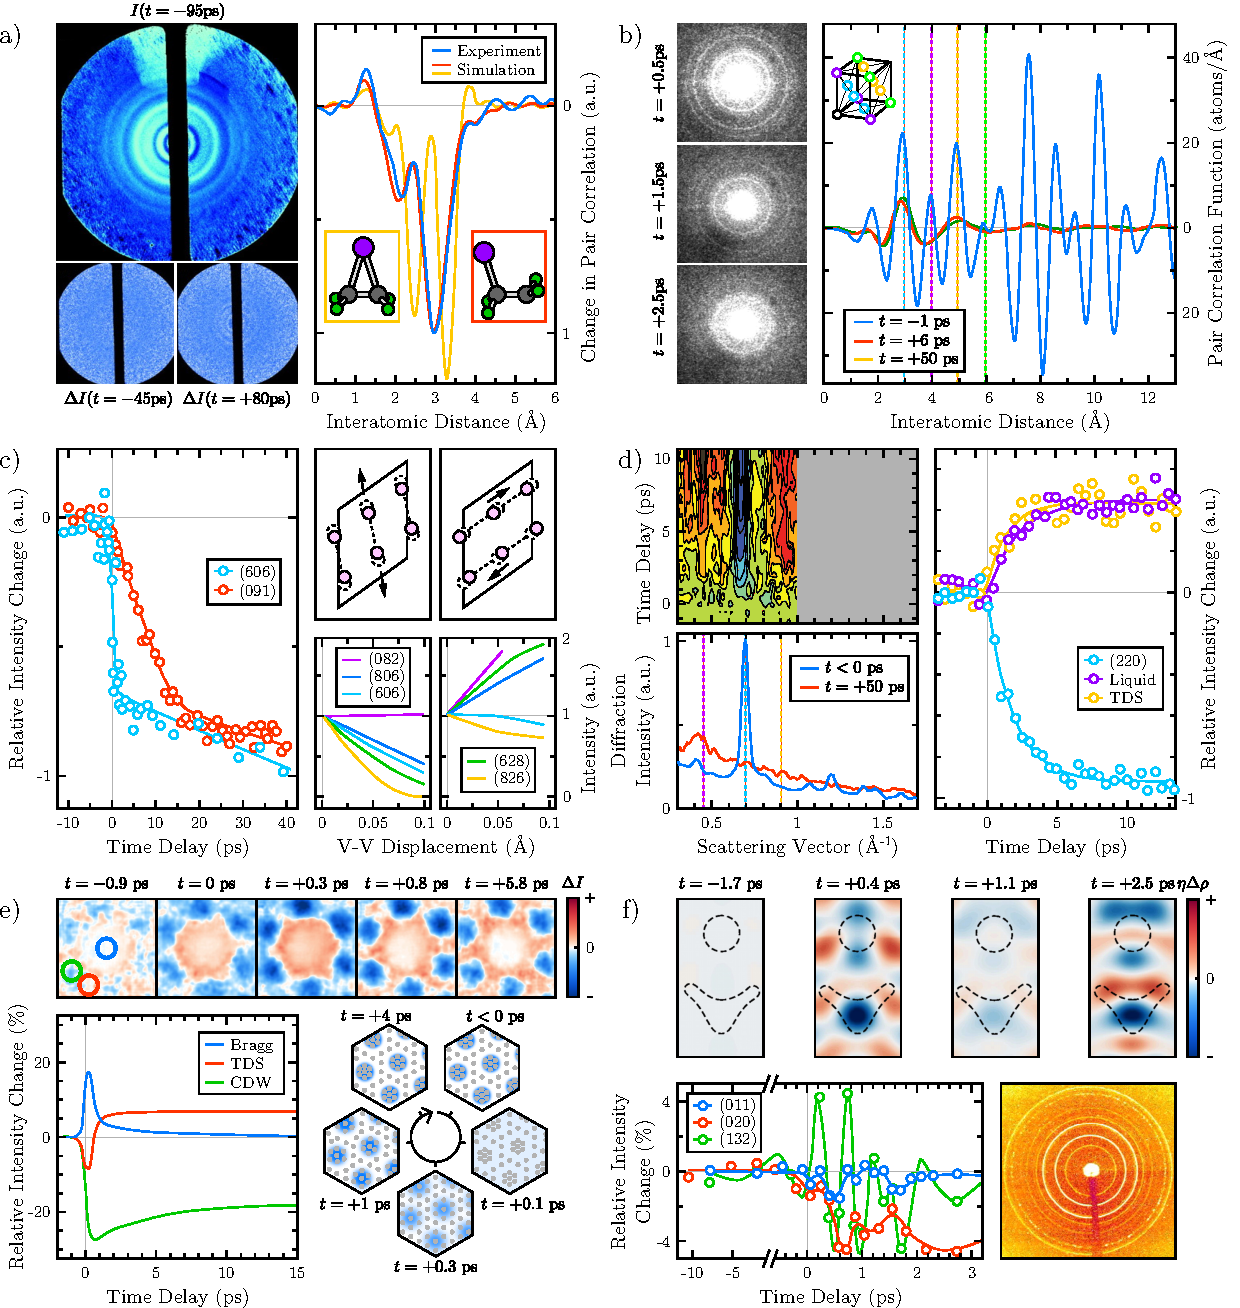
\includegraphics[width = \textwidth]{Figures/fig_intro_data.pdf}
  \caption[Making molecular movies by ultrafast diffraction.]{
    Making molecular movies by ultrafast diffraction:
    (a)~non-concerted elimination reaction in gas-phase $\mathrm{C_2 F_4 I_2}$;
    (b)~laser-induced melting of single-crystal aluminum;
    (c)~photoinduced phase transition in single-crystal {VO$_2$};
    (d)~laser-induced bond hardening of polycrystalline gold;
    (e)~optical suppression of charge density waves in single-crystal {1T-TaS$_2$};
    (f)~ultrafast charge transfer in powder KH$_2$PO$_4$.
    Adapted with permission from Refs.~\cite{Ihee2001, Siwick2003, Baum2007,
    Ernstorfer2009, Eichberger2010, Zamponi2012} respectively.
  }
  \label{fig: intro-data}
\end{figure}

% Describe previous UED works
Prior to my contributions in 2013,
several works in the literature have already answered the above question
in the affirmative for small molecules in the gas phase~\cite{Ihee2001},
highly symmetric materials~\cite{Baum2007, Eichberger2010, Zamponi2012},
and simple metals~\cite{Siwick2003, Ernstorfer2009}.
%
Some of their major results and approaches are summarized in Fig.~\ref{fig: intro-data}.
%
In Panel~(a), Ihee et~al~\cite{Ihee2001} determined the structure of a reaction intermediate
by calculating the change in pair correlation function from the difference diffraction pattern
and comparing it to that from two chosen structure models (`bridged' versus `classical').
%
In Panels~(b) and (d), Miller and co-workers~\cite{Siwick2003, Ernstorfer2009}
followed the laser-induced melting of two simple metals by directly interpreting
the time evolution of the correlation values of known atomic pairs
in a face-centered-cubic unit cell~\cite{Siwick2003} or the intensity of diffraction features
associated with the different phases (solid versus liquid) and
thermal diffuse scattering~(TDS)~\cite{Ernstorfer2009}.
%
In Panel~(c), Baum et~al~\cite{Baum2007} deduced the motion of the one asymmetric vanadium atom
in VO$_2$ crystals during its photoinduced phase transition
by considering the amplitude and sign of the intensity changes of 16 diffraction spots
and comparing them again to those calculated from the structure factor of
two likely structure models.
%
In Panel~(e), Eichberger et~al~\cite{Eichberger2010} observed the suppression and recovery
of charge density waves~(CDW) in the highly symmetric material {1T-TaS$_2$}
by observing the rise and fall in intensity of diffraction features associated with
the lattice order of the Ta~atoms (Bragg spots), disorder (inelastic background),
and the six-fold superlattice distortions caused by CDW (satellite spots).
%
Finally, in Panel~(f), Zamponi et~al~\cite{Zamponi2012} reconstructed the charge density distribution
of {KH$_2$PO$_4$} from powder XRD data by assuming that the 2D~inversion symmetries of the unit cell
are conserved and thus forcing the phase change of the structure factors
to always be either $0$ or $\pm \pi$.

% Caveats of above methods
In the above cases, the structural dynamics of the sample could be inferred so simply
because of the small number of asymmetric atoms.
%
As in Refs.~\cite{Ihee2001, Baum2007} and others,
such molecular systems have low degrees of freedom and thus
only a small number of structural ansatzes need to be tested.
%
Similarly, in highly symmetric crystals like simple metals~\cite{Siwick2003, Ernstorfer2009},
the space of interatomic distances is so sparse that
the atomic motions can be read out directly from peaks of the pair correlation function
calculated by a Fourier transform of the measured diffraction patterns.
%
In addition, the presence of conserved inversion symmetries,
as in Ref.~\cite{Zamponi2012} and similar works,%
\footnote{See Refs.~\cite{Zamponi2010, Woerner2010, Stingl2012, Zamponi2012b, Juve2013, Freyer2013}.}
means that there is not much a phase problem to solve:
the complex phase of the structure factors is therein fixed at $0$ or $\pm \unslant[-.2]\pi$.
%
Another simplifying consequence of these few-atom samples
is that they expectedly exhibit structural dynamics of low dimensionality
in terms of reaction coordinates;
most of the active atomic motions could be captured and discerned
by sampling only a small subset of diffraction spots in reciprocal space.
%
Lastly, the task of making molecular movies therein was made easier
by having the active atoms be strong scatterers --- e.g. V~\cite{Baum2007},
I~\cite{Ihee2001}, Ta~\cite{Eichberger2010}, Au~\cite{Ernstorfer2009}, Bi~\cite{Sciani2009} ---
which could afforded the higher signal-to-noise ratios~(SNR) necessary
for resolving subtle time-dependent changes in the diffraction data.

% Previous methods not applicable
The molecular systems whose results are described in this thesis
are non-trivial with respect to those studied prior in the literature.
%
They are mostly composed of weakly scattering carbon,
with ca.~$100$ atoms in a moderately sized unit cell%
\footnote{See App.~\ref{ap: cif} for their crystallographic information.} of lower symmetry,
chosen for the interesting photo-physics and chemistry that can be accessed
by laser excitation and acts as test~cases for proteins and other biological macromolecules
in more ambitious UED experiments of the future.
%
As such, these molecule movies cannot be made using the previously used tricks
and requires a new approach --- herein based on data science ---
that shall constitute the scientific question and answer of this thesis.

% Describe the phase problem of crystallography
% Figure: Cowtan's cat
% http://www.ysbl.york.ac.uk/~cowtan/fourier/coeff.html

% In the case of the experiment described in Sec.~\ref{sec: UED-AZA},
% 123,768 images --- $0.28$~TB --- were collected over 15 days.
% ($219.2$~kB/s)

% Streaking experiments (Carbone2012)
% Reflection experiments

% First paper on radial functions in electron diffraction (gas) \cite{Pauling1935, Debye1941}

% % 4th paradigm of science: data
% \cite{Agrawal2016}.


\section{Overview of Thesis}

% The goal of this thesis is to directly observe the ultrafast changes in structure of molecules
% during a chemical reaction using UED. In other words, it is to make
% a molecular movie with femtosecond time resolution and sub-angstrom spatial resolution.
% I will show that I have achieved this goal and made several significant contributions along the way,
% under the supervision of R. J. Dwayne Miller and in collaboration with many other colleagues.

Large portions of this thesis are based on works --- experiments and discussions ---
done in collaboration between several colleagues and me.
The results described herein have been previously published in the following articles:
%
\begin{itemize}
  \item M. Gao, C. Lu, H. Jean-Ruel, \underline{L. Liu}, A. Marx, K. Onda, S.-Y. Koshihara,
    Y. Nakano, X. Shao, T. Hiramatsu, G. Saito, H. Yamochi, R. R. Cooney, G. Moriena, G. Sciaini,
    and R. J. D. Miller,
    ``Mapping Molecular Motions Leading to Charge Delocalization with Ultrabright Electrons,''
    \textit{Nature}, vol.~496, pp.~343--346, 2013.

  \item H. Jean-Ruel, M. Gao, M. A. Kochman, C. Lu, \underline{L. Liu}, R. R. Cooney,
    C. A. Morrison, and R. J. D. Miller,
    ``Ring-Closing Reaction in Diarylethene Captured by Femtosecond Electron Crystallography,''
    \textit{J. Phys. Chem. B}, vol.~117, pp.~15894--15902, 2013.

  \item S. Manz, A. Casandruc, D. Zhang, Y. Zhong, R. A. Loch, A. Marx, T. Hasegawa,
    \underline{L. Liu}, S. Bayesteh, H. Delsim-Hashemi, M. Hoffmann, M. Felber, M. Hachmann,
    F. Mayet, J. Hirscht, S. Keskin, M. Hada, S. W. Epp, K. Fl\"{o}ttmann, and R. J. D. Miller,
    ``Mapping Atomic Motions with Ultrabright Electrons: Towards Fundamental Limits in Space-Time
    Resolution,'' \textit{Farad. Discuss.}, vol.~177, pp.~467--491, 2015.

  \item R. L. Field, \underline{L. Liu}, W. Gawelda, C. Lu, R. J. D. Miller,
    ``Spectral Signatures of Ultrafast Spin Crossover in Single Crystal
    [Fe\textsuperscript{II}(bpy)\textsubscript{3}](PF\textsubscript{6})\textsubscript{2},''
    \textit{Chem. Eur. J.}, vol.~22, pp.~5118--5122, 2016.

  \item Y. Jiang, \underline{L. Liu}, H. M. M\"{u}ller-Werkmeister, C. Lu, D. Zhang, R. L. Field,
    A. Sarracini, G. Moriena, E. Collet, and R. J. D. Miller,
    ``Structural Dynamics upon Photoexcitation in a Spin Crossover Crystal Probed
    with Femtosecond Electron Diffraction,''
    \textit{Ang. Chem. Int. Ed.}, vol.~56, pp.~7130--7134, 2017.

  \item \underline{L. Liu}, Y. Jiang, H. M. M\"{u}ller-Werkmeister, C. Lu, G. Moriena,
    M. Ishikawa, Y. Nakano, H. Yamochi, and R. J. D. Miller,
    ``Ultrafast Electron Diffraction Study of Single-Crystal
    (EDO-TTF)\textsubscript{2}SbF\textsubscript{6}: Counterion Effect and Dimensionality Reduction,''
    \textit{Chem. Phys. Lett.}, vol.~683, pp.~160--165, 2017.

  \item K. M. Krawczyk, R. L. Field, \underline{L. Liu}, M. Dong, A. Woolley, and R. J. D. Miller,
    ``Illuminating the Photoisomerization of a Modified Azobenzene Single Crystal
      by Femtosecond Absorption Spectroscopy,'' \textit{Can. J. Chem.}, vol.~97, pp.~488--495, 2019.

  \item Y. Jiang, \underline{L. Liu}, K. M. Krawczyk, A. Sarracini, J. S. Wentzell, Cheng Lu,
    R. L. Field, S. F. Matar, W. Gawelda, H. M. M\"{u}ller-Werkmeister, and R. J. D. Miller,
    ``Direct Observation of Nuclear Reorganization Driven by Ultrafast Spin Transitions,''
    2019 (under consideration).

\end{itemize}

In reflection of the multifaceted nature of my doctoral work,
this thesis is organized into a methods chapter (Ch.~\ref{ch: methods})
and several `science' chapters (Ch.~\ref{ch: UED-EDO}--\ref{ch: SCO})
that are each focused on the results reported in one of the above publications.

I will begin in Ch.~\ref{ch: methods} by describing the theoretical and experimental framework
of the two techniques used throughout these works:
transient absorption~(TA) spectroscopy and ultrafast electron diffraction.
I will give an overview of the physics of the relevant probe-matter interaction,
the experimental setup used to perform the measurements, and novel data analysis procedures that
I developed to extract weak signal from noisy datasets and reconstruct the relevant ultrafast dynamics
of the molecules under study.

In Ch.~\ref{ch: UED-EDO}, I will present experimental results on the ultrafast structural dynamics
of the family of molecules (EDO-TTF)\textsubscript{2}X, where X = PF\textsubscript{6}
and SbF\textsubscript{6}.
In the case of X = PF\textsubscript{6}, the experiment demonstrates that it is possible with UED to
resolve the atomic motions of an organic crystal as it reversibly undergoes
a photoinduced insulator-to-metal phase transition~\cite{Gao2013}.
The data analysis reveals the existence of a short-lived intermediate state whose formation involves
motions distinct from the thermal motions that drive later relaxation to the final state.
In the second half of the chapter, I will discuss results from a follow-up experiment,
where a much larger SbF\textsubscript{6} ion is substituted
for the PF\textsubscript{6} ion~\cite{Liu2017}. Here, I will examine the under-appreciated role
played by these spectator ions and focus on the consequences of this atomic replacement
on the structural dynamics of the EDO-TTF ions after photoexcitation.

In Ch.~\ref{ch: UED-DAE}, I will describe UED work on a class of organic molecules known
as diarylethenes (DAE)~\cite{Jean-Ruel2013}. This study focuses on directly observing
the photoinduced ring-closing reaction that occurs in this molecular system.
This photochemical process is a model system for understanding the reaction dynamics that involve
a crossing between potential energy surfaces through a conical intersection.
Analysis of the experimental results shows that a distinct open-ring intermediate state
is first formed through the activation of a small number of key motions on time scales
consistent with an earlier spectroscopic study~\cite{Jean-Ruel2011}.

In Ch.~\ref{ch: SCO}, I will examine the phenomenon of photoinduced spin crossover (SCO) in
two transition metal complexes:
[Fe\textsuperscript{II}(bpy)\textsubscript{3}](PF\textsubscript{6})\textsubscript{2}
and [Fe\textsuperscript{II}(PM-AzA)\textsubscript{2}(NCS)\textsubscript{2}]. Upon photoexcitation,
these molecules, denoted BPY and AZA respectively, undergo SCO, a transition from
a low-spin (LS) ground state to a metastable high-spin (HS) excited state. I will first
present the experimental results of the BPY study, where the spectral features of SCO
in single-crystal BPY are measured using femtosecond TA spectroscopy~\cite{Field2016}.
The observed excited-state dynamics are found to be initially similar with those determined
from aqueous BPY samples and are followed by slower behaviour that are clearly related
to crystal lattice effects.
In the latter half of the chapter, I will report the results of the AZA study,
where UED is used as a complementary tool to TA spectroscopy to explore the structural dynamics
associated with the SCO transition~\cite{Jiang2017}. Here, the focus is on the speed and timing of
three key atomic motions: metal--ligand bond elongation, ligand motion, and unit cell expansion.
Refinement of the UED data reveals that these modes are strongly coupled and are activated on
a timescale slower than that of the SCO electronic dynamics. This opens the question on
whether metal--ligand bond elongation and SCO transition are concomitant but not simultaneous.
Further discussions are presented here to explore the possibility that the structural feature
probed by UED is not a simple bond length change but the narrowing of an initially broad
bond length distribution.

In Ch.~\ref{ch: future}, I will present some notes on works that are either
currently in progress and yet to published, follow-ups to previous experiments,
or proposed for the future.
%
In particular, two projects are discussed:
(1)~a UED experiment to test the feasibility of rotation UED and charge flipping~(CF)
and (2)~a follow-up UED~study on SCO whereby BPY is probed instead of AZA~\cite{Jiang2019}.

In Ch.~\ref{ch: conclusion}, I will offer a summary of the main results and conclusions
of my doctoral work.

\section{Author's Contributions}

The work presented in this thesis was carried out as a result of several collaborations between myself
and a number of esteemed colleagues at various institutions. In this section, I would like to acknowledge
and describe the important contributions that they have made in helping
to bring the aforementioned projects to fruition.

The UED setup that is the subject of Sec.~\ref{sec: UED-setup} and used in the works described in
Chs.~\ref{ch: UED-EDO}--\ref{ch: future} was conceived by R. J. Dwayne Miller. It was designed,
built, and implemented by a number of former postdoctoral fellows and graduate students
in the Miller group: Maher Harb, Sergei Kruglik, Meng Gao, Hubert Jean-Ruel, Germ\'{a}n Sciaini, Gustavo Moriena,
and Ryan R. Cooney~\cite{Hubert-thesis, Gao2012}. I developed the instrument control and data acquisition
program that is currently in use for the experimental setup, with the assistance of Gustavo Moriena.
Furthermore, Cheng Lu prepared the ultrathin samples used in all the experiments via ultramicrotomy
from bulk single crystals. R. J. Dwayne Miller supervised all the projects and
co-authored the various manuscripts reporting on the project results.

The UED experiments on the structural dynamics of
single-crystal (EDO-TTF)\textsubscript{2}PF\textsubscript{6},
described in Sec.~\ref{sec: UED-EDOPF6}, were initially performed by Cheng Lu, Germ\'{a}n Sciaini,
and Gustavo Moriena at the University of Toronto. These were followed by more experiments that were led
by Meng Gao, Hubert Jean-Ruel, and Ryan R. Cooney. The crystals were synthesized and characterized
by our Japanese collaborators at the Tokyo Institute of Technology
(Ken Onda and Shin-ya Koshihara),
Kyoto University (Yoshiaki Nakano and Xiangfeng Shao, and Hideki Yamochi),
and Meijo University (Takaaki Hiramatsu and Gunzi Saito).
Alexander Marx determined the crystal orientation of the samples.
Meng Gao and I jointly analyzed the UED data and conceived the few-mode refinement model that
allowed the full recovery of the ultrafast structural dynamics of the molecule in the study.
Meng Gao and Germ\'{a}n Sciaini wrote the manuscript
while I contributed to the supplementary information~\cite{Gao2013}.

I led and initiated the follow-up UED experiment on (EDO-TTF)\textsubscript{2}SbF\textsubscript{6} that is
described in Sec.~\ref{sec: UED-EDOSbF6}. The crystals were synthesized using electrocrystallization
by Manabu Ishikawa and Yoshiaki Nakano, and Hideki Yamochi at Kyoto University.
Yifeng Jiang and Donald Kelloway collected the data and I analyzed it
in its entirety using my own techniques;
I also developed the concept of dimensionality reduction to interpret the results.
Ryan L. Field and Gustavo Moriena participated in helpful discussions to further the conclusions.
Yifeng Jiang and Henrike M. M\"{u}ller-Werkmeister, and I wrote
the manuscript reporting the results~\cite{Liu2017}.

The UED experiments on single-crystal diarylethene described in Ch.~\ref{ch: UED-DAE}
were performed by Hubert Jean-Ruel, Meng Gao, and Ryan R. Cooney. Hubert Jean-Ruel
and I developed the atomic-motion model and wrote the code used to analyze the UED data.
Michal A. Kochman and Carole A. Morrison at the University of Edinburgh
contributed to theoretical work that supported the model used in the data analysis.
Hubert Jean-Ruel wrote the manuscript reporting the results~\cite{Jean-Ruel2013}.

The femtosecond UV-Vis TA~spectroscopy experiments described
in Sec.~\ref{sec: TA-BPY} were performed and built by Ryan L. Field.
Wojciech Gawelda at the European X-ray Free Electron Laser provided us
the bulk crystals of [Fe\textsuperscript{II}(bpy)\textsubscript{3}](PF\textsubscript{6})\textsubscript{2}
for sample preparation via ultramicrotomy.
Ryan L. Field and I jointly analyzed and interpreted the TA data
using singular value decomposition~(SVD) and global analysis, which we then wrote up
for publication~\cite{Field2016}.

The UED experiments on single-crystal
[Fe\textsuperscript{II}(PM-AzA)\textsubscript{2}(NCS)\textsubscript{2}]
were performed by Yifeng Jiang, Henrike M. M\"{u}ller-Werkmeister,
Antoine Sarracini, and me.
Eric Collet at the Universit\'{e} de Rennes~1 provided the bulk crystals and
Dongfang Zhang at the Max Planck Institute for the Structure and Dynamics of Matter measured
the 800-nm transmittance of the samples at both room and cryogenic temperatures. Ryan L. Field and
Gustavo Moriena partipated in discussions to develop the interpretation. Yifeng Jiang and I analyzed
the UED data and developed the few-mode model for elucidating the ultrafast structural dynamics
of the sample. Yifeng Jiang, Henrike M. M\"{u}ller-Werkmeister,
and I wrote the manuscript reporting the results~\cite{Jiang2017}.

In Ch.~\ref{ch: future}, I described some works that are in progress and not yet published.
%
The concept of rotation UED described in Sec.~\ref{sec: rotation-CF} was conceived by me.
The (EDO-TTF)$_2$PF$_6$ data collected by sample tilting
--- using the same samples as in Sec.~\ref{sec: UED-EDOPF6} ---
was measured by Meng Gao and Yifeng Jiang and analyzed by me.
In particular, the very promising pump--probe geometry depicted in Fig.~\ref{fig: Rotation-schematic}c
was conceived by Ryan L. Field.
%
In Sec.~\ref{sec: UED-SVD}, I presented a novel approach to UED data analysis
that I conceived. Therein, the entire image stack
--- not the individual time traces calculated from each reciprocal lattice point ---
is dimensionally reduced by SVD. The demonstrative results shown in Fig.~\ref{fig: UED-SVD}
were obtained using the same UED data in Sec.~\ref{sec: UED-EDOPF6}.
%
Furthermore, in Sec.~\ref{sec: freq-anal-BPY},
I conceived and performed wavelet-based frequency analysis on the previous reported broadband TA results,
giving an unprecedented view of the oscillation dynamics in all three axes: time delay, probe wavelength,
and wavelet wavenumber.

Finally, the UED experiment on single-crystal [Fe$^\text{II}$(bpy)$_3$](PF$_6$)$_2$
in Sec.~\ref{sec: UED-BPY} was led and primarily performed by Yifeng Jiang,
with assistance from Kamil M. Krawczyk, Antoine Sarracini, Jordan S. Wentzell,
Henrike M. M\"{u}ller-Werkmeister, and me.
%
I analyzed the resulting data and constructed the four-mode refinement model from which
I made a molecular movie of the structural dynamics of BPY.
The bulk crystals were provided by Wojciech Gawelda and cut via ultramicrotomy
by Jordan S. Wentzell and Cheng Lu.
Samir F. Matar performed the quantum chemical calculations on BPY and AZA
that were used to support the conclusions drawn from the UED results.
%
Yifeng Jiang, Henrike M. M\"{u}ller-Werkmeister, and I wrote
the manuscript describing this work~\cite{Jiang2019}.



%

  
\chapter{Methods: Experimental Techniques and Data Science}
\label{ch: methods}

This chapter focuses on the methods --- experimental and analytical --- used to
attain the results presented in Ch.~\ref{ch: UED-EDO}--\ref{ch: conclusion}.
Here, two experimental techniques will be described in detail:
transient absorption~(TA) spectroscopy and ultrafast electron diffraction~(UED).
I will outline the theoretical framework of the probe-sample interaction
that is at the heart of each technique.
I will also give an overview of the instrumentation that makes up the lab setups
and detail the data-driven procedures used to characterize the experimental conditions,
correct measurement artifacts, improve signal-to-noise ratios, and finally extract the
relevant information from models for further interpretation.

%%%%%%%%%%%%%%%%%%%%%%%%%%%%%%%%%%%%%%%%%%%%%

\section{Transient Absorption Spectroscopy}
\label{sec: TA}

\subsection{Overview}
\label{sec: TA-overview}

In general, spectroscopy is the study of the interaction between materials and
different kinds of light in the electromagnetic spectrum.
By analyzing the shape of the resulting spectrum,
a sample can be studied and its structural and dynamical properties inferred.

In linear absorption spectroscopy, the sample is
illuminated by `probe' photons, which are selectively absorbed when
their energy $E = hc/\lambda$ coincides with the energy difference between
two quantum states of the correct symmetry;
the transmitted photons are spectrally resolved and counted using
a photodetector. The energy scale of this light-matter interaction determines
the physics that is probed. Absorption peaks that show
up in the ultraviolet~(UV) and visible~(Vis) regions correspond to transitions
between the electronic states of molecules. Similarly, excitations amongst
molecular vibrational and rotational states appear as features in the infrared~(IR)
and microwave parts of the spectrum. The amplitude of each peak is related to
the probability of the associated transition, which is proportional to
the square of the relevant transition moment integral.
Although the latter can be derived from time-dependent perturbation theory
and the input wavefunctions and energies approximated using various ab initio techniques,
disentangling the many overlapping features in the congested absorption spectrum of
a minimally complex molecular system is a serious challenge for any spectroscopist.

In this thesis, UV--Vis transient absorption spectroscopy is employed.
This technique is a pump-probe experiment,
wherein a small fraction of sample molecules are first excited
to a higher-lying electronic state by a narrow-bandwidth `pump' pulse.
After some time delay, a `probe' pulse spanning the UV--Vis spectrum arrives at the sample
to interrogate the dynamics of the excited state.
This pump-and-probe routine is repeated over a range of time delays
to produce a map of sample absorption as a function of time after photoexcitation.

Absorption of light by the sample is quantified by its absorbance~$A$,
which is defined as:
%
\begin{equation}
  A(\lambda) = -\log_{10} \left(  \frac{I_\text{trans}(\lambda)}{I_\text{inc}(\lambda)} \right)
\end{equation}
%
where $I_\text{trans}(\lambda)$ and $I_\text{inc}(\lambda)$
are the transmitted and incident intensities%
\footnote{Absorbance $A$ is often used interchangeably with the term
`optical density'~(OD); intensity $I$ refers to the irradiance of the laser~\cite{ISO9288}.}
as a function of probe wavelength $\lambda$, respectively. This quantity is related to
the physical properties of the sample via the Beer-Lambert law:
%
\begin{equation}
  A(\lambda) = c l \epsilon(\lambda)
\end{equation}
%
where $l$ is the optical path length of the sample,
$c$ is the molar concentration of the optically active species,
and $\epsilon (\lambda)$ is its wavelength-dependent absorption coefficient.

In TA spectroscopy, the absorption of the sample in the ground state is compared
with that after some time delay~$t$ following photoexcitation
by calculating the differential absorbance~$\Delta A(t, \lambda)$:
%
\begin{equation}
  \Delta A(t, \lambda) = A_\text{on}(t, \lambda) - A_\text{off}(\lambda) = -\log_{10} \left( \frac{I_\text{on}(t, \lambda)}{I_\text{off}(\lambda)} \right)
\end{equation}
%
where $A_p$ and $I_\text{p}$ are the sample absorbance and transmitted probe intensity,
given the state of the pump~$p \in \{ \text{on}, \text{off} \}$.
It is by studying the light-induced changes in $\Delta A$ that the electronic dynamics of the sample
can be elucidated.

\begin{figure}[t!]
  \centering
  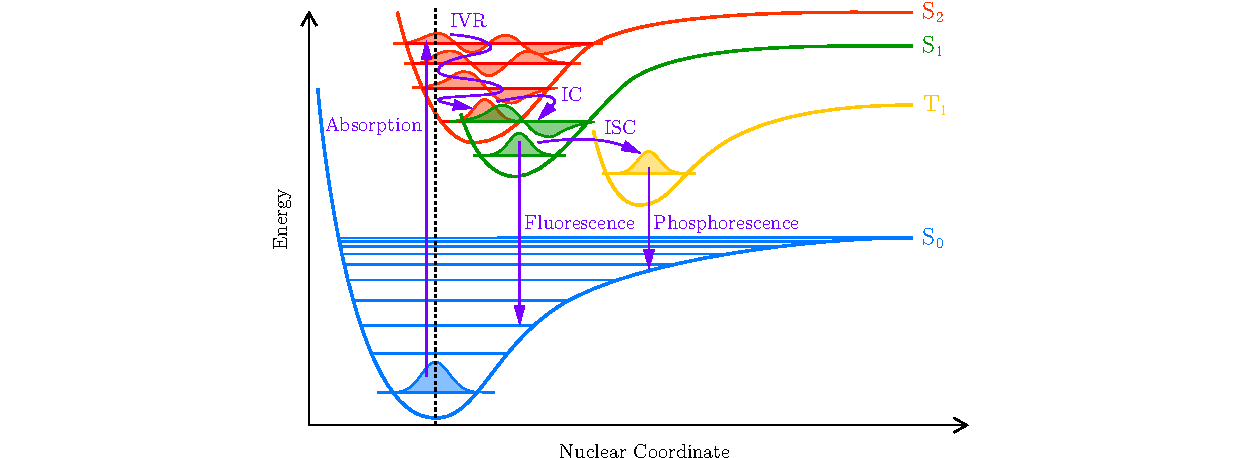
\includegraphics[width = \textwidth]{Figures/fig_ch2_photophysics.pdf}
  \caption[Illustration of the basic photophysical processes
  that can occur when light is absorbed by a molecule
  and the resulting photoexcited state relaxes back to the ground state.]{
  Illustration of the basic photophysical processes that can occur when light is
  absorbed by a molecule and the resulting photoexcited state relaxes back to the ground state.
  The potential energy curves of the first few molecular electronic states are shown:
  the ground state~($S_0$), first and second singlet excited states~($S_1$, $S_2$),
  and first triplet excited state~($T_1$).
  Some of the associated vibrational states are included as wavefunctions
  on a ladder of energy levels to highlight the relevance of wavefunction overlap
  in the Franck-Condon principle.
  Vertical and curved purple arrows indicate radiative and non-radiative transitions respectively;
  Abbreviations: IVR = intramolecular vibrational relaxation, IC = internal conversion,
  ISC = intersystem crossing.
  }
  \label{fig: photophysics}
\end{figure}

In Fig.~\ref{fig: photophysics}, some of the basic photophysical processes that
can be activated during an optical pump-probe experiment are shown.
Light absorption causes a transition from the electronic ground state $S_0$
to some electronic singlet excited state $S_2$.
Here, the Franck-Condon principle%
\footnote{Developed by James Franck (1882--1964) and Edward Condon (1902--1974) in 1926,
this principle states that an electronic transition is
most likely to occur without changes in the nuclear positions and
the transition probability is proportional to the square of the overlap integral between
the two vibrational wavefunctions involved~\cite{Franck1926, Condon1926}.\label{fn: franck-condon}}
determines which vibrational state of $S_2$ is more likely to be occupied initially.
The population of excited molecules can then decay through different
and competing relaxation pathways.
Some, like intramolecular vibrational relaxation~(IVR),
internal conversion~(IC), and intersystem crossing~(ISC), are non-radiative.
They respectively involve transitions between
vibrational states of the same electronic state,
electronic states of the same spin multiplicity, and
electronic states of different spin multiplicities.
Fluorescence and phosphorescence are the radiative equivalents of IC and ISC.
%
An empirical principle known as Kasha's~Rule%
\footnote{Originating from American spectroscopist Michael Kasha~(1920--2013)~\cite{Kasha1950}.
this `rule' is a consequence of the relative density of states
involved in these different types of vibrational-electronic (vibronic) transitions. \label{fn: Kasha}}
orders the time constant~$\tau$ of these transition as follows,
%
\begin{equation}
  \tau_\text{IVR} \ll \tau_\text{IC} \lesssim \tau_\text{ISC}, \tau_\text{F} \ll \tau_\text{P}
\end{equation}
%
Typical values of $\tau$ are shown in Tab.~\ref{tab: transitions} for reference.
%
\begin{table}[t!]
  \centering
  {\renewcommand{\arraystretch}{1.5}
  \begin{tabular}{l c c}
    \toprule
    Transition Process & Pathway & Time Scale~(s)\\
    \midrule
    Absorption & $ S_0 \rightarrow S_n $ & $<10^{-15}$ \\
    Vibrational Relaxation & $ S_n^* \rightarrow S_n $ & $10^{-13}$--$10^{-12}$ \\
    Internal Conversion & $ S_{n} \rightarrow S_{n'} $ & $10^{-14}$--$10^{-11}$ \\
    Intersystem Crossing & $ S_n \rightarrow T_n $ & $10^{-8}$--$10^{-3}$ \\
    Fluorescence & $ S_n \rightarrow S_0 $ & $10^{-9}$--$10^{-8}$ \\
    Phosphorescence & $ T_n \rightarrow S_0 $ & $10^{-3}$--$10^{1}$ \\
    \bottomrule
  \end{tabular}
  }
  \caption{Some general properties of the basic types of electronic transitions~\cite{Jaffe1966}.}
  \label{tab: transitions}
\end{table}

In a TA spectrum, various signals can appear.
%
Negative changes in sample absorption result from either ground state bleach~(GSB),
stimulated emission, or spontaneous emission. The first is a relative increase in
probe-light transmittance caused by depletion of ground-state molecules during pumping.
Stimulated emission is light emitted by electrons in the excited state
whose transition back to the ground state is enhanced by the probe pulse;
in contrast, spontaneous emission stems from probe-independent
radiative relaxation processes (e.g.~fluorescence and phosphorescence) and
are not temporally resolved in TA spectroscopy.
%
Positive changes in absorption are related to
excited state absorption~(ESA) and product state absorption~(PSA),
involving transitions from the excited states populated by the pump pulse to
even higher ones.
%
In addition, a strong signal is usually present
within the time interval when the pump and probe pulses overlap temporally and the combined
laser intensity is high enough to activate a nonlinear process known as
cross-phase modulation~(CPM).%
\footnote{For a more detailed description of CPM, see Ref.~\cite{Islam1987}.}
In Sec.~\ref{sec: TA-data-analysis}, a description is given on how this artifact and others
are removed.
Finally, any other process that changes the energy difference between optically active states
and/or the relevant transition probabilities can give rise to signals in TA data.

\subsection{Experimental Setup}
\label{sec: TA-setup}

The experimental setup for TA spectroscopy is illustrated in Fig.~\ref{fig: TA-setup}.
It is mainly composed of two parts: a commercial femtosecond laser system and
a home-built TA spectrometer.
%
The laser system is composed of
a femtosecond mode-locked laser oscillator (Coherent Micra-5~\cite{MicraManual})
and a titanium-doped sapphire (Ti:Sapph) regenerative amplifier
(REGEN, Coherent Legend Elite~\cite{LegendManual})
along with its high-energy Q-switched pump laser (Coherent Evolution-30~\cite{EvolutionManual}).

\begin{figure}[t!]
  \centering
  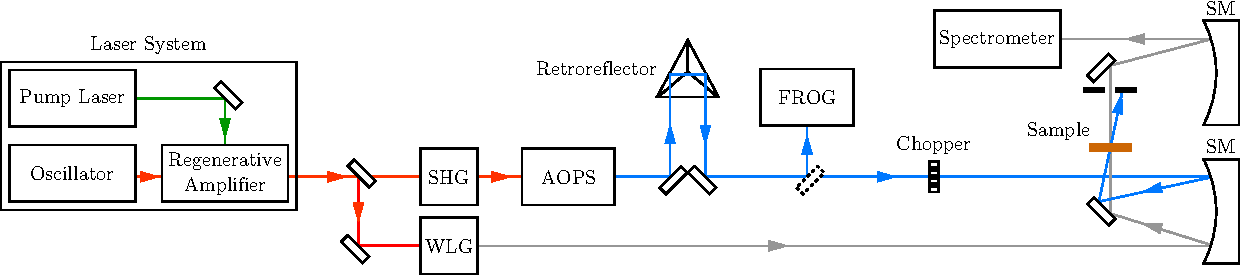
\includegraphics[width = \textwidth]{Figures/fig_ch2_setup-TA.pdf}
  \caption[Schematic of the experimental setup for TA spectroscopy.]{
    Schematic of the experimental setup for TA spectroscopy.
    For simplicity, it is not drawn to scale and minor components are not shown here.
    The directional lines represent optical beam paths and
    their colour denotes the wavelength
    (green = 527 nm, red = 800 nm, blue = 400 nm, and grey = 350--650 nm).
    Abbreviations: SHG = second harmonic generation, WLG = white light generation,
    AOPS = acousto-optic pulse shaper, FROG = frequency-resolved optical gating,
    SM = spherical concave mirror.
  }
  \label{fig: TA-setup}
\end{figure}

During operation, ultrashort seed pulses from the oscillator are strongly amplified in the REGEN
through chirped pulse amplification~(CPA) using light from the pump laser~\cite{Strickland1985}.
%
First light comes from inside the Micra-5 laser:
an intracavity frequency-doubled neodymium-doped yttrium orthovanadate (Nd:YVO\textsubscript{4})
continuous~wave laser (Coherent Verdi) pumps a Ti:Sapph oscillator with green light at 532 nm;
through Kerr-lens mode-locking,%
\footnote{Scottish physicist John Kerr (1824--1907) discovered in 1875 that
the index of refraction of material can be modified by an electric field to the second order:
$\Delta n \propto |\boldsymbol{E}|^2$.
Kerr-lens modelocking involves an optical pulse so intense that it self-focuses
under its own induced $\Delta n$ and is self-selected when coupled with an aperture
that blocks any other mode that fails to self-focus~\cite{BoydBook}.}
weak ultrashort pulses of red light at 800 nm are generated
with a repetition rate of 80 MHz. This pulse train enters the REGEN,
where it is chirped (i.e.~broadened in time) by a grating-based pulse stretcher.
One pulse (out of 8 $\times$ 10\textsuperscript{4}) is selected and injected
into the cavity of the REGEN by a Pockels%
\footnote{German physicist Friedrich Pockels (1865--1913) discovered in 1893 that
the index of refraction of material can be modified by an electric field to the first order:
$\Delta n \propto |\boldsymbol{E}|$. This effect can be used to quickly and precisely control
the polarization of a light beam~\cite{BoydBook}.} cell.
Concurrently, strong green light (537-nm center wavelength, 250-ns pulse duration, 20-mJ pulse energy,
1-kHz repetition rate) from the frequency-doubled
neodymium-doped yttrium lithium fluoride (Nd:YLF) Evolution-30 laser pumps
the Ti:Sapph crystal in the REGEN cavity.
The seed pulse undergoes multiple round trips in the cavity,
accumulating energy from the gain medium each time.
Once the pulse can no longer be further amplified,
it is ejected from the cavity by a second Pockels cell, recompressed by a pulse compressor,
and allowed to leave the REGEN. This output pulse has the following characteristics:
800-nm center wavelength, 35-fs pulse duration, 3.5-mJ pulse energy, and 1-kHz repetition rate.

Light from the laser system is now split into two beams, one going into the `pump' arm
and the other into the `probe' arm of the optical setup. Briefly, the pulses in the former:
frequency-doubled to 400 nm via second harmonic generation~(SHG)%
\footnote{SHG is a nonlinear optical process whereby two photons with the same frequency interact in
a medium to generate a single photon with double the frequency~\cite{BoydBook}.}
in a beta barium borate~(BBO) crystal, compressed using an acousto-optic pulse shaper~(AOPS)~\cite{Dugan1997},
time-delayed by passing through a delay line consisting of a retroreflector mounted on a motorized
translation stage, characterized using a frequency-resolved optical gating device~(FROG)~\cite{Trebino2000},
gated using an optical chopper to set the pump condition, focused onto the sample,
and finally dumped onto a beam block.
%
Simultaneously, the pulses in the probe arm are:
spectrally broadened via white light generation~(WLG)%
\footnote{WLG is the conversion of laser light into light with a very broad spectral bandwidth
(spanning hundreds of nanometers) via strongly nonlinear interactions
in a medium~\cite{Alfano1970, Nagura2002}.}
in a \(\mathrm{CaF_2}\) crystal,
focused onto the sample where it spatially overlaps with the focal spot of the pump beam,
recollimated, and passed into the home-built spectrometer.
%
With the exception of the laser system, the entire experimental setup here
was designed and built by Dr.~Ryan L. Field as part of his doctoral project.
Further details can be found in his thesis~\cite{Ryan-thesis}.

\subsection{Data Analysis}
\label{sec: TA-data-analysis}

During a TA experiment, there are significant features
in the data that are caused by optical processes of no present interest. They are artifacts
that need to be removed before the $\Delta A(t, \lambda)$ measurements are studied too closely.
In Fig.~\ref{fig: TA-Clean}, sample TA data at different stages of artifact removal
are shown and the parameters used to quantify the contribution of the artifacts are plotted alongside.
%
\begin{figure}[t!]
  \centering
  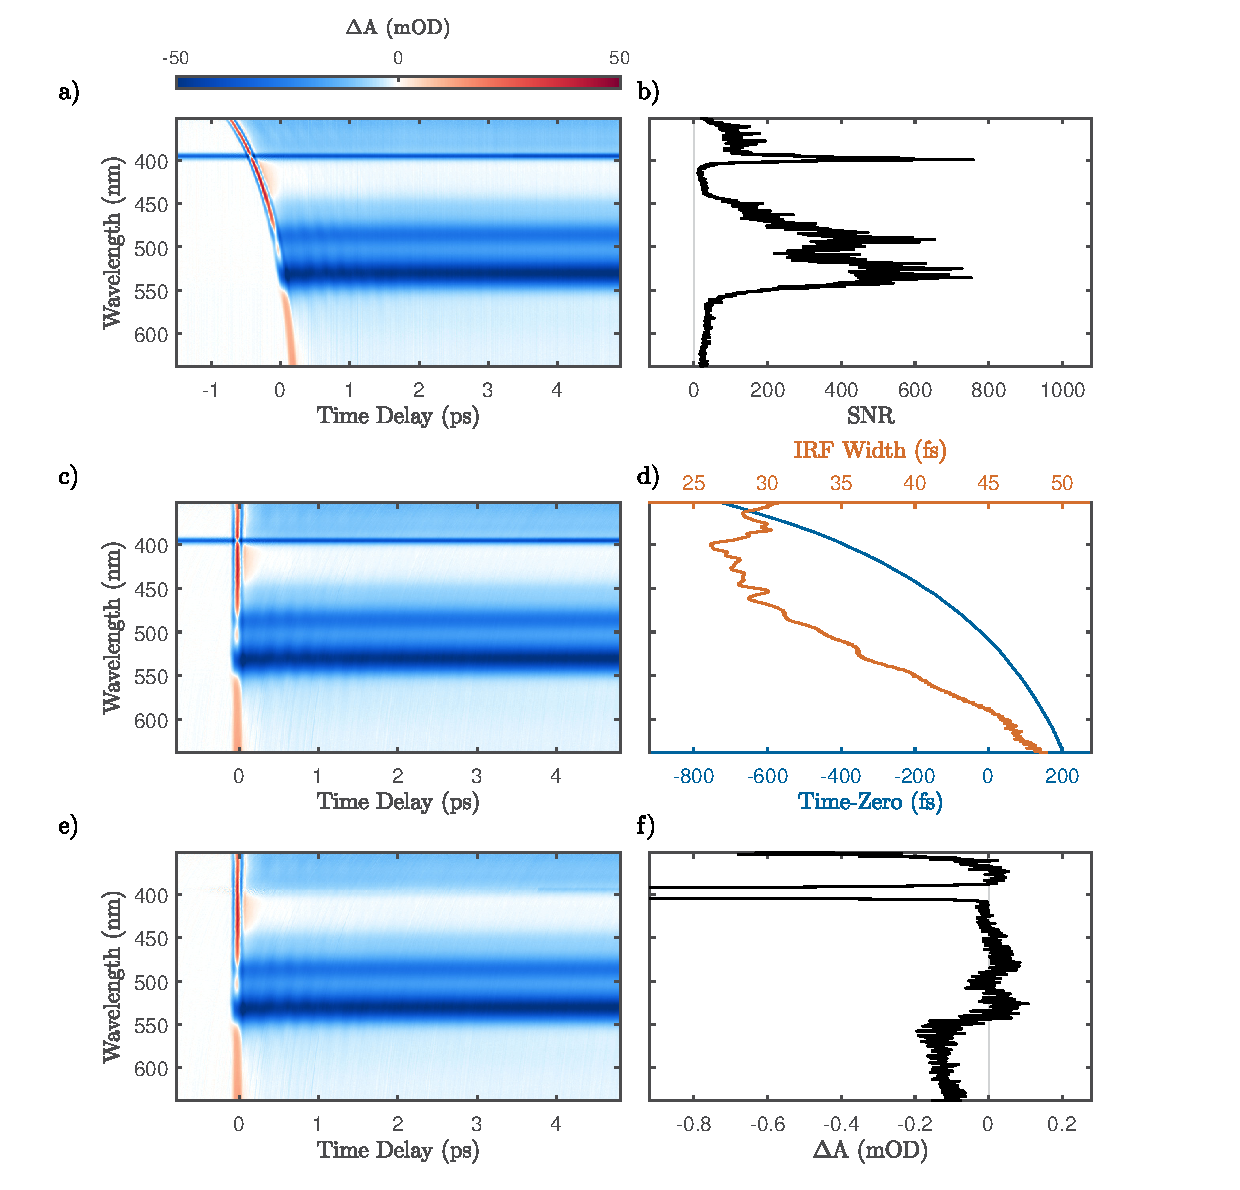
\includegraphics[width = \textwidth]{Figures/fig_TA_cleanup.pdf}
  \caption[Illustration of the steps for artifact removal in TA data.]{
  Illustration of the steps for artifact removal in TA data.
  Step 1: (a) restrict TA data to wavelength regions where $\textrm{SNR}(\lambda) > 5$
  using (b) the SNR estimated from Eq.~\eqref{eq: mu-sigma-SNR} for all probed wavelengths.
  Step 2: (c) correct the GVD distortion of the TA data
  by reversing (d) the wavelength dependence of the time-zero and IRF~width
  derived from a Hermite fitting of the CPM signal as in Eq.~\eqref{eq: CPM-fit}.
  Step 3: (e) obtain the final artifact-free TA data by
  (f) integrating and then subtracting all pre-CPM signals via Eq.~\eqref{eq: pre-signal}.
  }
  \label{fig: TA-Clean}
\end{figure}

The first step is the removal of regions of low signal-to-noise ratio~(SNR)
in the wavelength domain. This is caused by the fact that the bandwidth of white-light probe
is finite and there is not enough light beyond to differentiate signal from noise (see Fig.~\ref{fig: BPY-data-whitelight}).
Here, the SNR is estimated to be the ratio of the mean~$\mu$ to the standard deviation~$\sigma$
of the differential absorbance measurements at late time delays $t \in [t', t'']$,
when all transient signals have decayed completely:
%
\begin{equation}
  \begin{aligned}
    \mu(\lambda) & = \frac{1}{T} \int_{t'}^{t''} \Delta A(t, \lambda) \mathrm{d}t  \\
    \sigma(\lambda) & = \sqrt{\frac{1}{T} \int_{t'}^{t''} \left( \Delta A (t, \lambda) - \mu(\lambda) \right)^2 \mathrm{d}t}
    \label{eq: mu-sigma-SNR}
  \end{aligned}
\end{equation}
%
where $T = t'' - t'$.
A window is then applied on the TA data by limiting its wavelength domain to an interval
in which the SNR is above a threshold value,
$\lambda \rightarrow \lambda \in \left\{ \lambda \mid \textrm{SNR}(\lambda) > 5 \right\}$.

Next, the wavelength-dependent shift in time-zero%
\footnote{`time-zero' is the time delay at which there is temporal overlap of the pump and probe pulses.}
is considered. This varying arrival time of the probe pulse is caused by group velocity dispersion~(GVD)
that occurs when the broadband probe light propagates through transmissive optical elements
of the experimental setup. To quantify this effect, TA measurements are made on samples%
\footnote{For the experiments described in Sec.~\ref{sec: TA-BPY}, the non-resonant samples
are just blank sample media: deionized water in a quartz flow cell for the aqueous case,
a sapphire window for the crystal case.} that are not resonant
within the probe wavelength region~(see Ref.~\cite{Ryan-thesis} for more details).
The correct time-zero~$t_0(\lambda)$ is estimated by fitting
the CPM~signal $\Delta A_\textrm{CPM}(t, \lambda)$ with a model function that is
a linear combination of the first four Hermite polynomials~$H_n$ for each wavelength:
%
\begin{equation}
  \textrm{C}(t, \lambda, \{a_n\}, t_0, \tau) =
    \sum_{n = 0}^4 a_n(\lambda) H_n(x) \Bigg\rvert_{x = (t - t_0(\lambda))/\tau(\lambda)}\\
  \label{eq: CPM-fit}
\end{equation}
%
Then, each time series of the sample data is translated temporally
such that all the time-zeros are aligned: $\Delta A(t, \lambda) \rightarrow \Delta A(t - t_0, \lambda)$.
For time-zero shifts which are not integer multiples of the time delay step size,
super-resolution alignment is achieved through spline interpolation.
Incidentally, the parameter $\tau(\lambda)$ corresponds to the temporal width
of the instrument response function (IRF)%
\footnote{The IRF here is assumed to be Gaussian, given that it is a convolution of
the nearly Gaussian temporal profile of the pump and probe pulses.} of the experimental
setup~\cite{Megerle2009}.

Another TA artifact is the negative signals caused by scattered pump light
and fluorescence from the sample. Since they occur independently of the probe pulse
and their amplitude is mostly determined by the geometry of the experimental setup,
they are present and nearly constant at all time delays. Thus, they are
removed by averaging the pre-CPM differential absorbance and subtracting it
from the rest of the TA values:
%
\begin{equation}
  \Delta A(t, \lambda) \rightarrow \Delta A(t, \lambda) - \frac{1}{T}\int_{t'}^{t''} \Delta A(t, \lambda) \mathrm{d} t
  \label{eq: pre-signal}
\end{equation}
%
where $t \in [t', t'']$ and $T = t'' - t'$ refer to the time delay interval before time-zero
during which the CPM~signal is not yet present

Now that the TA data is artifact-free, a technique known as global analysis (GA)
is applied to reduce $\Delta A(t, \lambda)$ into a sum of exponentially decaying
spectral components that could be assigned to specific electronic states
and photophysical processes~\cite{Nagle1991, Grondelle2004, Wilderen2011, Ruckebusch2012}.
The first step of GA is to recognize that $\Delta A(t , \lambda)$ is just a
$ M \times N$ data matrix $\mathbf{\Delta \! A}$, where $M$ and $N$ are the number of wavelength
and time points respectively,
%
\begin{equation}
\begin{aligned}
  %t & = \{ t_1, ..., t_N \} \\
  %\lambda & = \{ \lambda_1, ..., \lambda_M \} \\
  \Delta A(t, \lambda) \rightarrow \mathbf{\Delta \! A} =
  \begin{bmatrix}
      \Delta A(t_1, \lambda_1) & \cdots & \Delta A(t_N, \lambda_1) \\
      \vdots & \ddots & \vdots \\
      \Delta A(t_1, \lambda_M) & \cdots & \Delta A(t_N, \lambda_M)
  \end{bmatrix}
\end{aligned}
\end{equation}
%
and it can be factored using singular value decomposition~(SVD) into
separate spectral and temporal features:
%
\begin{equation}
  \mathbf{\Delta \! A} = \mathbf{U} \mathbf{S} \mathbf{V}^\mathsf{T}
\end{equation}
%
where $\mathbf{U} = U(\lambda)$ and $\mathbf{V} = V(t)$ are
orthogonal matrices of size $M \times M$ and $N \times N$ respectively;
$\mathbf{S}$ is a $M \times N$ diagonal matrix of rank $P$.
This factorization can be rewritten to give an expansion of $\mathbf{\Delta \! A}$
as a weighted ordered sum of `singular components' $\mathbf{X}_i$:
%
\begin{equation}
  \begin{aligned}
    \mathbf{\Delta \! A} & = \sum_{i = 1}^P s_i \mathbf{X}_i \\
    \mathbf{X}_i & = \mathbf{u}_i \otimes \mathbf{v}_i^\mathsf{T}
    \label{eq: TA SVD sum}
  \end{aligned}
\end{equation}
%
where $\mathbf{u}_i = u_i(\lambda)$ and $\mathbf{v}_i = v_i(t)$
are the column vectors of $\mathbf{U}$ and $\mathbf{V}$; they are known as
the left and right `singular vectors' and, specifically in TA, the `basis spectra'
and `kinetic traces' of the overall dataset, respectively; $s_i$ is defined as the diagonal entries of $\mathbf{S}$
and known as the `singular values' of the data matrix.
In general, the set of singular values is sorted in descending order and
an approximation of the data matrix can be obtained by truncating this summation
at some $P' \ll P$, thus keeping only those singular components that contribute
significantly to the overall signal. This concept is particularly useful in
deconvolving incoherent noise from signals and it is illustrated in Figure~\ref{fig: TA-SVD}.

\begin{figure}[t!]
  \centering
  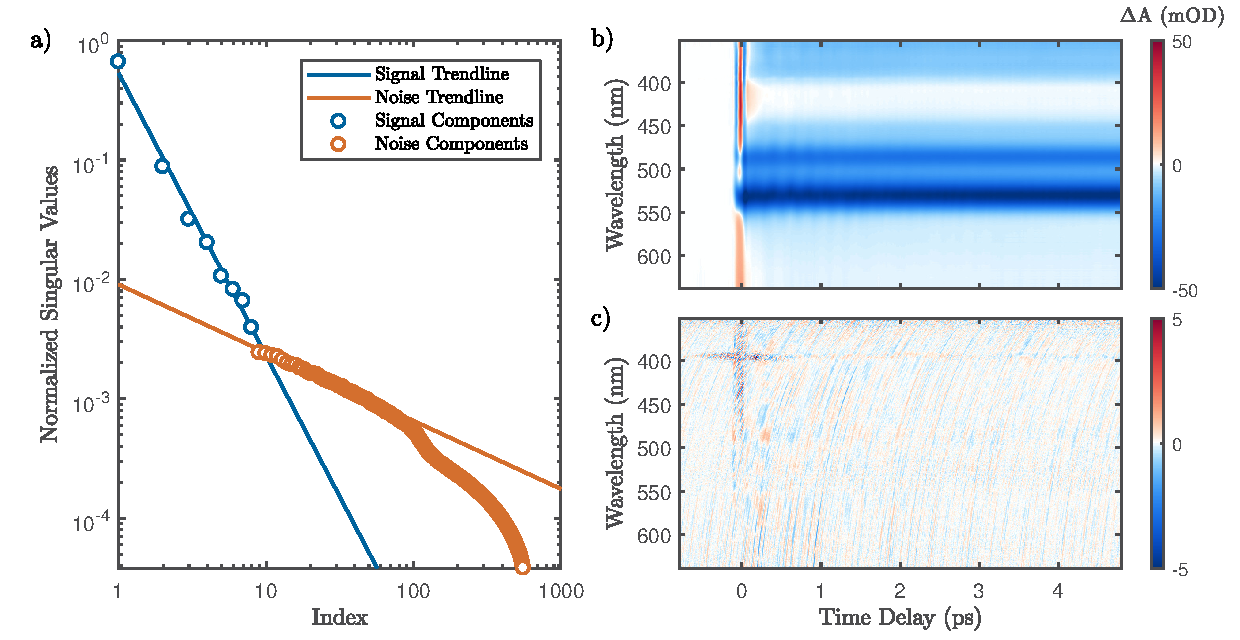
\includegraphics[width = \textwidth]{Figures/fig_TA_svd.pdf}
  \caption[Demonstration of a low-rank approximation of a TA data matrix using SVD.]{
  A low-rank approximation of a data matrix using SVD, as per Eq.~\eqref{eq: TA SVD sum},
  is demonstrated using the TA data shown in Fig.~\ref{fig: TA-Clean}f.
  The contribution of each singular component $\mathbf{X}_i$ is weighted by
  the associated singular value $s_i$,
  which is shown here on a log-log plot in (a)~after normalization.
  Two linear trendlines can be fitted piecewise to this curve; they are overlain
  to highlight the sudden change in slope as the normalized singular values decay to zero.
  Summing the singular components before and after this flexion yields
  the $\Delta A(t, \lambda)$ values in Panels~(b) and (c) respectively.
  By inspection, it is clear that the index at which the flexion occurs marks
  the point beyond which the remaining $\mathbf{X}_i$ only contribute irrelevant features
  and incoherent noise.
  }
  \label{fig: TA-SVD}
\end{figure}

After SVD and truncation, the TA dataset is now reduced to
a few basic spectra~$u_i(\lambda)$ and kinetic traces $v_i(t)$.
These are not readily interpretable in terms of photophysical processes
since they are only orthogonal bases that jointly span the data matrix.
To proceed further, a global lifetime analysis~(GLA) fit is done by assuming
an exponential model for the population dynamics of optically active species.
Each kinetic trace is assumed to be a weighted sum of $Q$ exponential decay functions
switched on at time-zero by a Heaviside step function $H(t)$ and convolved with a Gaussian IRF
whose temporal width $\tau_\text{IRF}$ is obtained earlier by fitting the response of
a non-resonant sample (see Fig.~\ref{fig: TA-Clean}f);
as before, the CPM~signal is described by a linear combination of the first four Hermite polynomials $H_n(t)$,
%
\begin{equation}
  \begin{aligned}
    C_i(t, \{a_{i n}\})
      & = \sum_{n = 0}^4 a_{i n}(\lambda) H_n \left( t/\tau_{\text{IRF}} \right)  \\
    \textrm{IRF}(t)
      & = \text{e}^{-\frac{1}{2} t^2/ \tau_\text{IRF}^2}  \\
    E_i(t, \{ b_{i j}\}, \{k_j\})
      & = \sum_{j = 1}^Q b_{i j} \left( H(t) \text{e}^{-k_j t}\right) \ast \text{IRF}(t) \nonumber\\
    f_i(t, \{a_{i n}\}, \{ b_{i j}\}, \{k_j\})
      & = C_i(t, \{a_{i n}\}) + E_i(t, \{ b_{i j}\}, \{k_j\})
    \label{eq: GA fit}
  \end{aligned}
\end{equation}
%
where $f_i$, $C_i$ and $E_i$ are the model functions for the kinetic trace $\boldsymbol{v}_i(t)$, and
its CPM and exponential contributions.%
\footnote{For reference,
$ \left( H(t - t_0) \text{e}^{-k t}\right) \ast \text{e}^{- \frac{1}{2} t^2/\tau^2} =
\frac{1}{2} \text{e}^{\frac{1}{2} k^2 \tau^2 - k (t - t_0)}
\left( 1 +
\text{erf}\left( \frac{t - t_0 - k \tau^2}{\sqrt{2} \tau} \right)
\right)$.
} To track the changes in $\Delta A$ that are associated with each exponential process,
a decay-associated spectrum (DAS) $D_j(\lambda)$ for each decay constant $k_j$
is calculated as a linear combination of the basis spectra $u_i(\lambda)$
weighted by the fitted amplitude $b_{i j}$ and singular values $s_i$:
%
\begin{equation}
  D_j(\lambda) = \sum_{i = 1}^{P'} b_{ij} s_i u_i(\lambda)
  \label{eq: DAS}
\end{equation}
%
This calculation is demonstrated using the TA data in Fig.~\ref{fig: TA-SVD}b and
the results are plotted in Fig.~\ref{fig: TA-GLA}.
%
\begin{figure}[ht!]
  \centering
  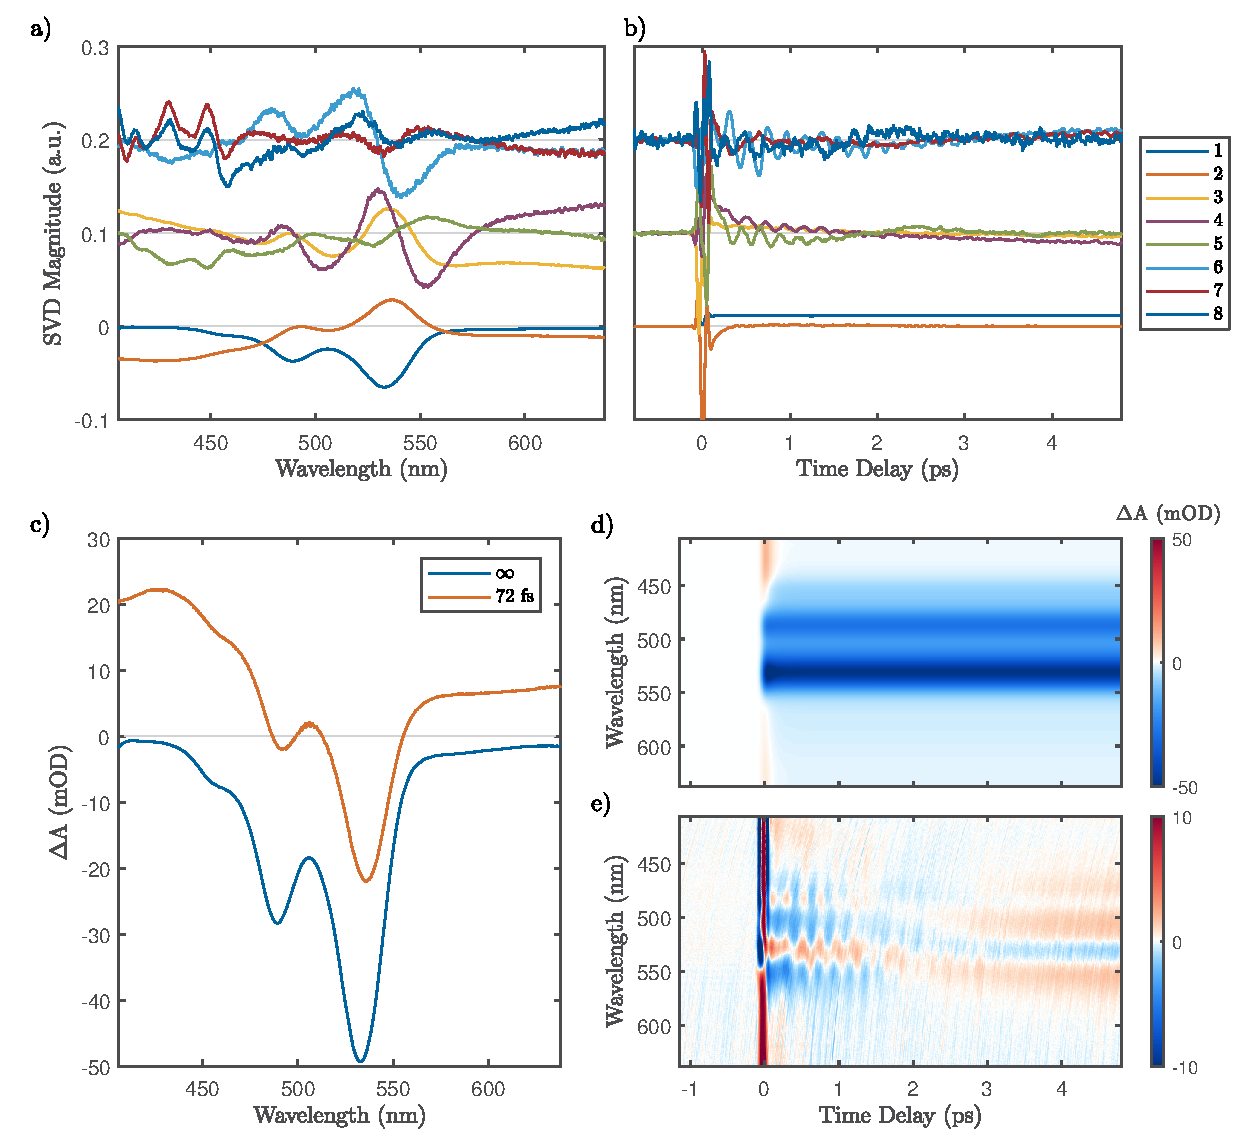
\includegraphics[width = \textwidth]{Figures/fig_TA_GLA.pdf}
  \caption[Truncation of a SVD sum at the point of flexion.]{
    Truncating the SVD sum of the TA data matrix (from Fig.~\ref{fig: TA-SVD}c)
    at the point of flexion leaves (a)~eight principal basis spectra and (b)~eight kinetic traces
    in the TA data matrix. Two exponential components ($\tau_1$ = $\infty$, $\tau_2$ = 72 fs)
    are needed for the GLA~fit of the kinetic traces (Eq.~\eqref{eq: GA fit})
    and their respective DAS (Eq.~\eqref{eq: DAS}) are plotted in Panel~(c).
    The resulting global fit and residuals are shown in Panels~(d) and (e).
  }
  \label{fig: TA-GLA}
\end{figure}
%
Finally, the global fit $G(t, \lambda)$ (as shown in Fig.~\ref{fig: TA-GLA}d)
are calculated by recombining each $D_j(\lambda)$ with
its corresponding exponential function with decay constant $k_j$:
%
\begin{equation}
  G(t, \lambda) = \sum_{j = 1}^{Q} D_j(\lambda) \left[  \left( H(t) \text{e}^{-k_j t}\right) \ast \textrm{IRF}(t) \right]
\end{equation}
%
The residuals of the fit, $R(t, \lambda) = \Delta A(t, \lambda) - G(t, \lambda)$, contain
signals not captured by the exponential model. As seen in Fig.~\ref{fig: TA-GLA}e, these features
include the CPM near time-zero, lattice heating effects at late times, and various oscillatory dynamics
in between. For the latter, relevant frequencies can be extracted by calculating
the power spectrum of the residuals at each probe wavelength
using Welch's method for spectral density estimation~\cite{Welch1967}
or a continuous wavelet transform (see Sec.~\ref{sec: freq-anal-BPY}).


%%%%%%%%%%%%%%%%%%%%%%%%%%%%%%%%%%%%%%%%%%%%%%%%%%%%%%%%%%%%%%%%%%%%%%%%%%%%%%%%%%%%%%%%%%%%%%%%%%%%%%

\section{Ultrafast Electron Diffraction}
\label{sec: UED}

Since its discovery in 1923--1927~\cite{Gehrenbeck1978}, electron diffraction became
an indispensable weapon in the arsenal of those seeking to
investigate the structure of materials on the atomic level.
%
The advent of time-resolved laser spectroscopy and the introduction of the pump--probe methodology
involving ultrashort pulses to this technique further extended its capabilities,
which now includes the study of ultrafast atomic motions and structural dynamics
during physico-chemical processes,
hence conferring it the titular specialization of ultrafast electron diffraction~(UED).

Given the roots of UED, some basic tenets of crystallography and electron scattering physics
is necessary to fully understand UED as an experimental technique and interpret its measurements.
%
As such, a brief introduction to these two topics ---
based on Refs.~\cite{AshcroftBook, EwaldBook, XRDBook, WarrenBook}
and~\cite{TownsendBook, CowleyBook, ReimerBook, KirklandBook, ZouBook, Giacovazzo2011} ---
is given as follows.

\subsection{Overview of Crystallography}
\label{sec: UED-cryst}

A common feature of physical objects is that
their constituent atoms are not distributed randomly
but are bound together as molecules and arranged in a regular periodic array.
Materials structured as such are known as crystals%
\footnote{Since the discovery of `quasicrystals' in 1984 by Israeli material scientist
Daniel Shechtman (1941--present)~\cite{Shechtman1984}, crystals are now more accurately described as
``any solids having an essentially discrete diffraction diagram''
wherein 3D~periodicity may be absent~\cite{IUC1992}.} and
they are the subject of study for crystallographers.

A fundamental concept to describe crystal structures is the `Bravais lattice',%
\footnote{Moritz L. Frankenheim (1801--1869) first discovered in 1826 that
they are no more than 15 distinct types of lattices in three dimensions.
Auguste Bravais (1811--1863) later correctly revised this number to 14~\cite{XRDBook}.}
which is an infinite array of points that maps back onto itself
under discrete translations in three-dimensional space.
The position of every point in a Bravais lattice can be stated as
$\boldsymbol{R} = n_1 \boldsymbol{a}_1 + n_2 \boldsymbol{a}_2 + n_3 \boldsymbol{a}_3$,
where $n_j$ are integers and $\boldsymbol{a}_j$
are the three non-coplanar primitive vectors that generate the lattice.
The region of space spanned by the vectors $\boldsymbol{a}_j$
is known as the `unit cell' of the lattice;
it is the spatial volume that is repeated throughout the lattice
and preserved under its translational symmetry.
Although there is no unique way to choose the primitive vectors and
the unit cell of a lattice,
the conventional approach is to pick the most orthogonal set of
lattice-generating vectors and the parallelepiped in the first octant
of the resulting coordinate system.
As seen in Fig.~\ref{fig: unit-cell}a, the unit cell and its primitive vectors are specified
by a set of six lattice parameters%
\footnote{In conventional crystallographic notation, the six lattice parameters are
denoted by $a, b, c, \alpha, \beta, \gamma$ respectively.
Here, this is done using the index notation for convenience.}:
the length of the three vectors ($a_1, a_2, a_3$)
and the internal angles ($\alpha_{23}, \alpha_{31}, \alpha_{12}$),
where $\cos \alpha_{ij} = | \hat{\boldsymbol{a}}_i \cdot \hat{\boldsymbol{a}}_j|$.
Herein, the components of $\boldsymbol{a}_j$ can be expressed as
%
\begin{equation}
\begin{aligned}
  \boldsymbol{a}_1 & = a_1 \left[ 1 \quad 0 \quad 0 \right]  \\
  \boldsymbol{a}_2 & = a_2 \left[ \cos \alpha_{12} \quad \sin \alpha_{12} \quad 0 \right] \\
  \boldsymbol{a}_3 & = a_3 \left[ \cos \alpha_{31} \quad \frac{\cos \alpha_{23} - \cos \alpha_{31} \cos \alpha_{12}}{\sin \alpha_{12} } \quad \frac{V}{a_1 a_2 a_3 \sin \alpha_{12}} \right]
\end{aligned}
\end{equation}
%
where $V$ is the volume of the unit cell,
%
\begin{equation}
\begin{aligned}
  V & = \left| \boldsymbol{a}_1 \cdot (\boldsymbol{a}_2 \times \boldsymbol{a}_3) \right| \\
    & = a_1 a_2 a_3 \sqrt{1 + 2 \cos \alpha_{23} \cos \alpha_{31} \cos \alpha_{12} - \cos^2 \alpha_{23} - \cos^2 \alpha_{31} - \cos^2 \alpha_{12}}
\end{aligned}
\end{equation}

\begin{figure}[t!]
  \centering
  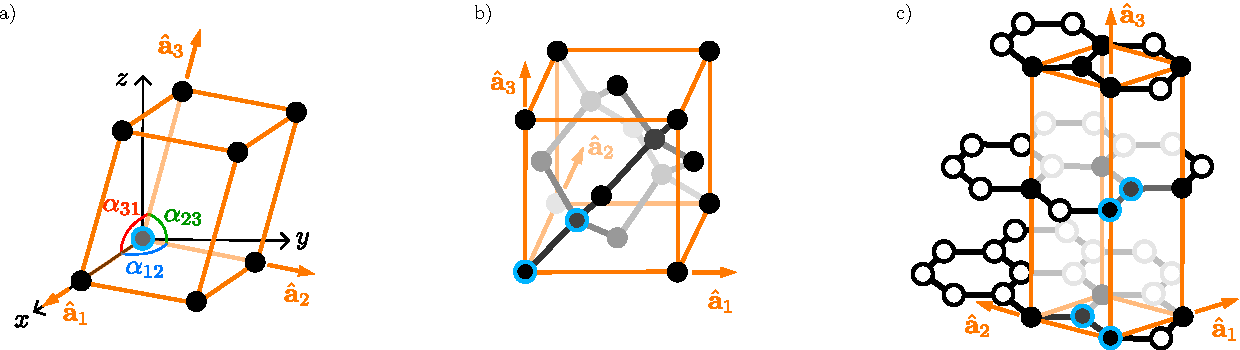
\includegraphics[width = \textwidth]{Figures/fig_ch2_unitcell.pdf}
  \caption[Crystal structures as described by their Bravais lattice.]{
    Crystal structures as described by a Bravais lattice and an associated basis.
    The unit cell is orange parallelepiped; atoms inside/outside are filled/empty circles;
    the basis atoms are outlined in blue.
    (a)~The six parameters ($a_1, a_2, a_3, \alpha_{23}, \alpha_{31}, \alpha_{12}$)
    that specify the shape of an unit cell are defined.
    The crystal structures of (b)~diamond and (c)~hexagonal graphite are depicted.
    The first is a face-centered cubic lattice with a two-atom basis;
    the second is a hexagonal lattice with a four-atom basis.
  }
  \label{fig: unit-cell}
\end{figure}

The structure of a physical crystal can be described
by a Bravais lattice wherein the repeating arrangement of atoms
is enclosed within the volume of a particular unit cell and
this subset of atoms defines a `basis' relative to each lattice point.
Under this scheme, the position of any atom $j$ in the crystal is given by
$\boldsymbol{r}_j = \boldsymbol{R}_{n_1 n_2 n_3} + \boldsymbol{\scriptr}_i$,
where $\boldsymbol{R}_{n_1 n_2 n_3} = \sum \limits_{j = 1}^3 n_j \boldsymbol{a}_j$
is the position of the lattice point to which the origin of the unit cell is defined
and $\boldsymbol{\scriptr}_i$ is the position of the basis atom $i$ that is equivalent
to atom $j$ under symmetry.

The facets of the crystal are related to families of parallel equidistant planes
which intersect the Bravais lattice at (at least) three non-collinear lattice points.
Within the unit cell, such a lattice plane has intercepts $\frac{a_j}{h_j}$ on the three lattice vectors
and can be specified by the notation $(h_1 h_2 h_3)$, where $h_j$ are coprime integers
(see Fig.~\ref{fig: reciprocal-laue-bragg}a) and they are known as the `Miller indices'%
\footnote{William H. Miller (1801--1880) introduced this notation for crystal planes in 1839.
The letters $h, k, l$ are used therein most often;
however, the labels $h_1, h_2, h_3$ are used instead here for convenient indexing.
An overline indicates a negative number, $\overline{h} = -h$.} of the plane.
A set of vectors can be constructed%
\footnote{A computationally more useful definition of the reciprocal lattice vectors is
$ \left[ \boldsymbol{b}_1 \boldsymbol{b}_2 \boldsymbol{b}_3 \right] = 2 \unslant[-.2]\pi \left[ \boldsymbol{a}_1 \boldsymbol{a}_2 \boldsymbol{a}_3 \right]^{-1}$,
where the vectors are in column representation.}
as $\boldsymbol{b}_i = \frac{\unslant[-.2]\pi}{V} \sum \limits_{j,k = 1}^3 \epsilon_{ijk} \enskip \boldsymbol{a}_j \times \boldsymbol{a}_k$,
where $\epsilon_{ijk}$ is the Levi-Civita symbol.
%
Under this definition, the three vectors $\boldsymbol{b}_i$ have the property of
$\boldsymbol{b}_i \cdot \boldsymbol{a}_j = 2 \unslant[-.2]\pi \delta_{ij}$, where $\delta_{ij}$ is the Kronecker delta,
with the corollary $|\boldsymbol{b}_i| = 2\unslant[-.2]\pi / |\boldsymbol{a}_i|$.
%
Since their magnitude is the reciprocal of that of the crystal lattice and
they can generate their own Bravais lattice
where each vector $\boldsymbol{g} = \sum \limits_{i = 1}^3 h_i \boldsymbol{b}_i$,
the vectors $\boldsymbol{b}_i$ are known as `reciprocal lattice vectors';
the reciprocal vector $\boldsymbol{g}$ corresponds to the normal of a plane $(h_1 h_2 h_3)$
in the `direct lattice' (as opposed to the reciprocal lattice)
and its magnitude is proportional to the reciprocal of the interplanar distance $d_{h_1 h_2 h_3}$,
$| \boldsymbol{g} | = 2\unslant[-.2]\pi/d_{h_1 h_2 h_3}$.
This geometric relationship between planes in the crystal lattice and
points in the reciprocal lattice provides a convenient basis to discuss
the interference of waves reflected by the bulk crystal.
%
\begin{figure}[t!]
  \centering
  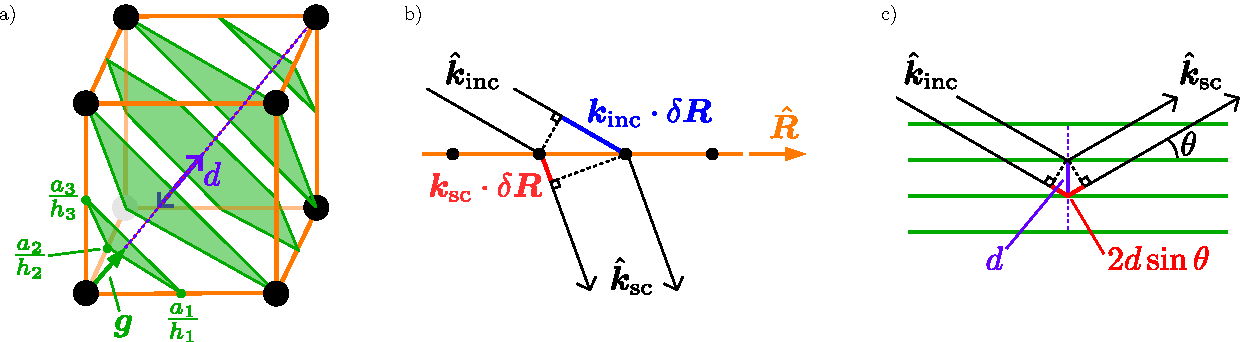
\includegraphics[width = \textwidth]{Figures/fig_ch2_reciprocal-laue-bragg.pdf}
  \caption[Diffraction according to Max v. Laue and William L. Bragg.]{
    (a) Family of lattice planes specified by the Miller indices $h_1, h_2, h_3 = 2$ is depicted,
    along with the reciprocal lattice vector $\boldsymbol{g}$ that corresponds to the normal of the planes.
    The path difference that leads to diffraction in crystals is shown
    according to the formulation of (b)~Max v. Laue and (c)~William L. Bragg.
  }
  \label{fig: reciprocal-laue-bragg}
\end{figure}

When a wave penetrates a material, new waves are produced through scattering and
they can interact with the original wave. In the case of a crystal, the periodic features
that underlie the crystal structure generate many scattered waves with discrete phase differences.
Under certain conditions, there is constructive interference between these waves and the incident one
and diffraction occurs. There are two formulations of these diffraction conditions:
one conceived by Max v. Laue and the other by William L. Bragg, both%
\footnote{Max v. Laue (1879--1960) was awarded the 1914 Nobel Prize in Physics for
the discovery of X-ray diffraction.
William L. Bragg (1890--1971), along with his father William H. Bragg (1862--1942),
won the same award in 1915 for their work in X-ray crystallography~\cite{Nobel1901}.} in 1912.
As seen in Fig.~\ref{fig: reciprocal-laue-bragg}b,
the first approach considers the crystal to be lines of scatterers,
equally spaced by $\delta \boldsymbol{R} = \boldsymbol{a}_j$;
assuming elastic scattering,
the phase difference between the transmitted wave and the scattered one
is $\Delta \phi = (\boldsymbol{k}_{\text{sc}} - \boldsymbol{k}_{\text{inc}}) \cdot \delta \boldsymbol{R}$
and thus, the Laue condition for diffraction is
%
\begin{equation}
  \boldsymbol{q} \cdot \boldsymbol{a}_j = 2 \unslant[-.2]\pi h_j
  \label{eq: laue}
\end{equation}
%
where $\hbar \boldsymbol{q} = \hbar(\boldsymbol{k}_{\text{sc}} - \boldsymbol{k}_{\text{inc}})$
is the momentum transferred during the scattering event and $h_j$ are integers.
In the Bragg formulation (Fig.~\ref{fig: reciprocal-laue-bragg}c), the crystal is composed of parallel reflective planes
evenly separated by the interplanar distance $d$; the incident wave interferes
with the reflected waves only if the path difference is an integer multiple $n$ of the wavelength $\lambda$
and hence the Bragg condition for diffraction is
%
\begin{equation}
  2 d \sin \theta = n \lambda
  \label{eq: bragg}
\end{equation}

The Laue and Bragg conditions are equivalent and this can be shown
by noting that the Laue condition effectively constrains
diffraction to only occur for $\boldsymbol{k}_\text{sc}$ such that
$\boldsymbol{q}$ is an integer multiple of a reciprocal lattice vector $\boldsymbol{g}$ of the crystal.
A helpful way to interpret these conditions is through
a geometric construct%
\footnote{Paul P. Ewald (1888--1985) conceived of the sphere-in-reciprocal-lattice construct
to geometrically visualize diffraction in 1912~\cite{EwaldBook}.} known as the `Ewald sphere'.
In the space of wavevectors, the reciprocal lattice
and a sphere --- centered on $\boldsymbol{k}_\textrm{inc}$ and
of radius $|\boldsymbol{k}_\textrm{inc}|$ ---
are drawn such that the latter is tangential to the lattice origin.
The surface of this sphere represents all possible elastic scattering events
such that $|\boldsymbol{k}_\textrm{sc}| = |\boldsymbol{k}_\textrm{inc}|$.
As seen in Fig.~\ref{fig: ewald}, the locations on the surface of the Ewald sphere that overlap
with any points of the reciprocal lattice specifies those scattering geometries
wherein the transfer wavevector $\boldsymbol{q}$ and the scattering $\theta$
satisfy the Laue and Bragg conditions respectively.
Propagating these beams onto the detector yields
the spots of the diffraction pattern that can be expected by an observer in real space.
%
\begin{figure}[t!]
  \centering
  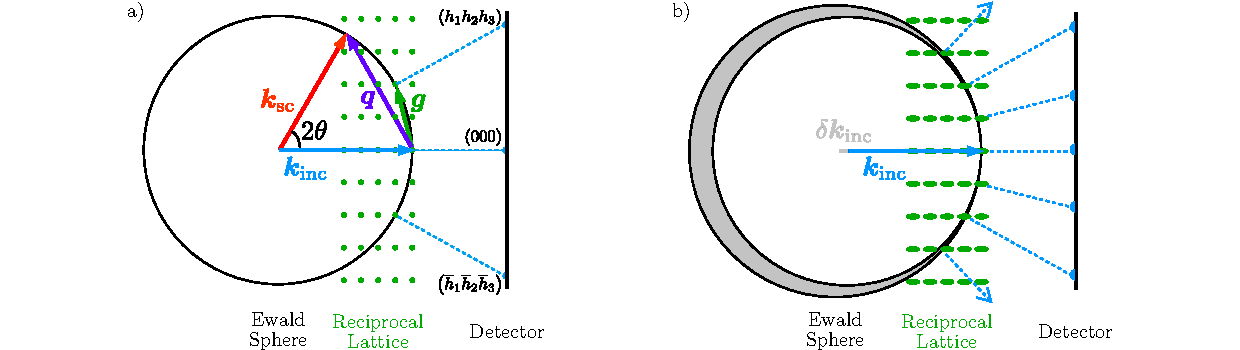
\includegraphics[width = \textwidth]{Figures/fig_ch2_ewald.pdf}
  \caption[Construction of the Ewald sphere.]{
    Construction of the Ewald sphere.
    (a)~The Laue-Bragg condition is satisfied at scattering angles $\theta$
    where the surface of the sphere coincides with reciprocal lattice points $\boldsymbol{g}$;
    when projected onto the detector, these points indicate where diffraction spots may be observable.
    (b)~Realistic incident beams with nonzero energy and momentum spreads,
    in addition to finite and imperfect crystals,
    loosen the condition for diffraction and lead to more diffraction spots
    than would otherwise be expected.
  }
  \label{fig: ewald}
\end{figure}

In a perfect, infinite, and static crystal,%
\footnote{A `perfect' crystal is one with unbroken discrete translational symmetry;
`infinite' refers to the absence of boundaries, and `static', a lack of atomic motion.}
few if any diffraction spots would be observable
for a general monochromatic incident beam.
It is unlikely that any integer solution $(h_1 h_2 h_3)$,
other than the transmitted beam at $(000)$,
exactly satisfies the Laue-Bragg condition.
In practice, incident beams are not composed of
perfectly coherent waves;
the resulting nonzero energy and momentum spread manifest
within the Ewald construct (Fig.~\ref{fig: ewald}b)
as a thickening the surface of the sphere into a shell
that can overlap with many more reciprocal lattice points.
Furthermore, the finite dimensions and long-range disorder
of the crystal effectively broaden the points into extended spikes%
\footnote{These shapes are known in the literature as
reciprocal lattice rods, or `relrods' for short.}
that can more easily be intercepted by the Ewald sphere.
Hence, experimental imperfections ensure that
the requirements of diffraction are sufficiently relaxed
for a multitude of spots to appear in a diffraction pattern.

\begin{figure}[ht!]
  \centering
  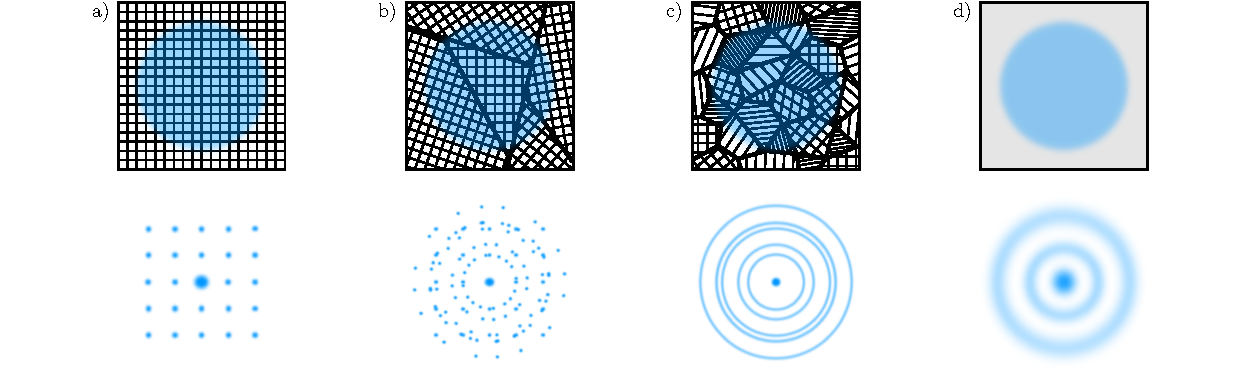
\includegraphics[width = \textwidth]{Figures/fig_ch2_crystal-powder-diff.pdf}
  \caption[Samples of varying crystallinity and the resulting diffraction patterns.]{
    Samples of varying crystallinity and the resulting diffraction patterns:
    (a)~a perfect single crystal, (b)~a polycrystal, (c)~a powder,
    and (d)~an amorphous sample.}
  \label{fig: crystal-powder-diff}
\end{figure}

A diffraction pattern does not necessarily appear as
the regular array of spots that the Ewald construct would suggest.
The nature of the pattern can be an indication of the crystallinity
of the target. As shown in Fig.~\ref{fig: crystal-powder-diff},
a perfect single crystal gives a periodic arrangement of diffraction spots
while fluids and amorphous%
\footnote{An amorphous material is one that lacks the long-range order of
a crystal.} materials produce highly diffuse rings centered around the transmitted beam.
%
In between these two extremes in structural order,
there are coarse- and fine-grained polycrystalline materials
wherein the individual randomly-oriented crystallites contribute
their own diffraction spots that sum to a set of spotty concentric circles,
generally known as Debye-Scherrer%
\footnote{Paul Scherrer (1890--1969), under the guidance of Peter Debye (1884--1966), and
Albert W. Hull (1880--1966) developed in 1915--1917 the method for analyzing
X-ray crystal structures using powder samples
instead of single-crystal ones~\cite{EwaldBook, DebyeScherrer2011}.
\label{fn: debye-waller}} rings.

\subsection{Physics of Electron Scattering}
\label{sec: UED-physics}

\begin{figure}[ht!]
 \centering
 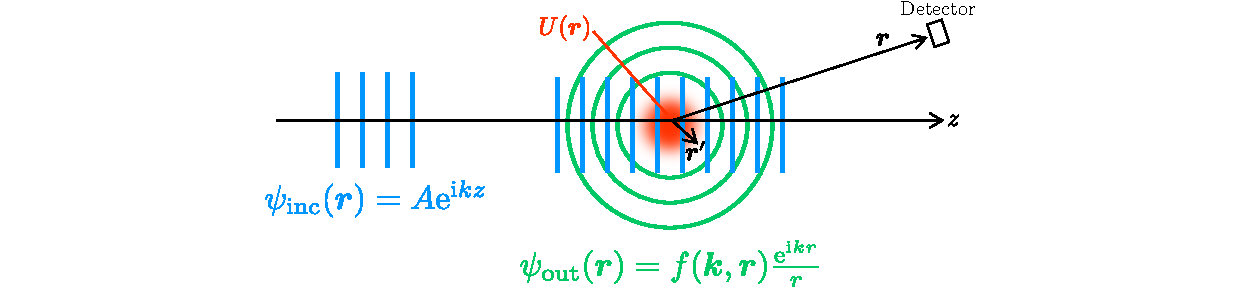
\includegraphics[width = \textwidth]{Figures/fig_ch2_electron-scatter.pdf}
 \caption{
  Schematic of the geometry of a prototypical three-dimensional scattering experiment.
 }
 \label{fig: electron-scatter}
\end{figure}

The Laue-Bragg condition determines the geometry
in which waves scattered by a crystal can constructively interfere
and give rise to diffraction.
To calculate the amplitude of these waves,
consider a prototypical scattering experiment:
a free electron impinging on a single atom in three dimensions.
As depicted in Fig.~\ref{fig: electron-scatter},
the incident matter wave $\psi_{\text{inc}}(\boldsymbol{r})$
is taken to be a plane wave traveling along the $z$ axis and
the scattered wavefunction is a linear combination of the original plane wave and
an outgoing spherical wave that is produced by the interaction:
%
\begin{equation}
  \begin{aligned}
    \psi(\boldsymbol{r}) & \sim \psi_{\text{inc}}(\boldsymbol{r}) + \psi_{\text{out}}(\boldsymbol{r}) \\
      & = A \text{e}^{\text{i} k z} + f(\boldsymbol{k}, \boldsymbol{r}) \frac{\text{e}^{\text{i} k r}}{r}
    \label{eq: sc1}
  \end{aligned}
\end{equation}
%
where $f(\boldsymbol{r}, \boldsymbol{k})$ is the scattering amplitude of the interaction.
%
To calculate the scattering amplitude, let us start with the time-independent Schr\"{o}dinger%
\footnote{Erwin Schr\"{o}dinger (1887--1961) won the 1933 Nobel Prize in Physics
along with Paul A. M. Dirac for formulating the wave equation
that now bears his name~\cite{Nobel1901}.} equation,
%
\begin{equation}
  \left( -\frac{\hbar^2}{2 m_e} \nabla^2 + U(\boldsymbol{r}) \right) \psi(\boldsymbol{r}) = E \psi(\boldsymbol{r})
\end{equation}
%
where $m_e$ is the mass of the electron, $U(\boldsymbol{r})$ is the electrostatic potential energy of the atom.
This can be re-written as
%
\begin{equation}
\begin{aligned}
  \left( \nabla^2 + k^2 \right) \psi(\boldsymbol{r}) & = \frac{2 m_e}{\hbar^2} U(\boldsymbol{r}) \psi(\boldsymbol{r}) \\
  L \psi(\boldsymbol{r}) & = \frac{2 m_e}{\hbar^2} U(\boldsymbol{r}) \psi(\boldsymbol{r})
\end{aligned}
\end{equation}
%
where $k = \sqrt{2 m_e E}/\hbar$ is the magnitude of the wavevector of the incident electron and
$L$ is the linear differential operator $\nabla^2 + k^2$.
A formal solution of this equation can be expressed as
%
\begin{equation}
  \psi(\boldsymbol{r}) = \psi_0(\boldsymbol{r}) + \frac{2 m_e}{\hbar^2} \int G(\boldsymbol{r}, \boldsymbol{r}^\prime) U(\boldsymbol{r}^\prime) \psi(\boldsymbol{r}^\prime) \mathrm{d}^3 r^\prime
  \label{eq: formal}
\end{equation}
%
where $\psi_0(\boldsymbol{r})$ is a solution of the homogeneous equation $L \psi(\boldsymbol{r}) = 0$ and
$G(\boldsymbol{r}, \boldsymbol{r}^\prime)$ is the Green's function%
\footnote{George Green (1793--1841) made important contributions to mathematical physics
in an essay on electricity and magnetism in 1828; these include the relationship between
properties inside a volume and those on its surface (Green's theorem) and a potential function
that can be used to impose boundary conditions (Green's function)~\cite{GreenWhy, GreenBio}.}
 of $L$,
i.e.~a solution of the equation $L \psi(\boldsymbol{r}) = \delta^3 (\boldsymbol{r} - \boldsymbol{r}^\prime)$.
Solving these two coupled differential equations yields
%
\begin{equation}
  \begin{aligned}
    \psi_0(\boldsymbol{r}) & = A \text{e}^{\text{i} k z} \\
    G(\boldsymbol{r}, \boldsymbol{r}^\prime) & = -\frac{\text{e}^{\text{i} k | \boldsymbol{r} - \boldsymbol{r}^\prime |}}{4 \unslant[-.2]\pi | \boldsymbol{r} - \boldsymbol{r}^\prime |}
    \label{eq: greenfunc}
  \end{aligned}
\end{equation}
for some constant $A$.
%
Since the atomic potential energy $U(\boldsymbol{r})$ is highly localized to microscopic distances,
the range of the $\boldsymbol{r}^\prime$ integral is limited to the region of $r^\prime \ll r$ and
some approximations can be made by neglecting terms of order $(r^\prime / r)^2$ and higher as
%
\begin{equation}
  | \boldsymbol{r} - \boldsymbol{r}^\prime | = r \sqrt{ 1 - \hat{\boldsymbol{r}} \cdot \frac{\boldsymbol{r}^\prime}{r} + \left(\frac{r^{\prime}}{r} \right)^2 } \approx r \left( 1 - \hat{\boldsymbol{r}} \cdot \frac{\boldsymbol{r}^\prime}{r} \right)
\end{equation}
%
and similarly,
%
\begin{equation}
  \frac{1}{| \boldsymbol{r} - \boldsymbol{r}^\prime |} \approx \frac{1}{r}
\end{equation}
%
Furthermore, the energy $E$ of the incident electrons in a UED experiment is about $10^5$ eV,
whereas the atomic potential energy $U$ is on the order of $10^1$--$10^2$ eV;
Given that $E \gg |U|$, the Born approximation can be applied to the expression for the scattered wavefunction
by replacing $\psi(\boldsymbol{r}^\prime)$ with $\psi_0(\boldsymbol{r}^\prime) \propto \text{e}^{\text{i} k z^\prime}$.
Therefore, by substituting in Eq.~\eqref{eq: greenfunc} and applying these approximations,
Eq.~\eqref{eq: formal} becomes
%
\begin{equation}
  \begin{aligned}
    \psi(\boldsymbol{r})
      & = A \text{e}^{\text{i} k z} + \frac{2 m_e}{\hbar^2}
        \int \left( -\frac{\text{e}^{\text{i} k | \boldsymbol{r} - \boldsymbol{r}^\prime |}}{4 \unslant[-.2]\pi | \boldsymbol{r} - \boldsymbol{r}^\prime |} \right)
        U(\boldsymbol{r}^\prime) \psi(\boldsymbol{r}^\prime) \mathrm{d}^3 r^\prime \\
      & \approx A \text{e}^{\text{i} k z} + \frac{2 m_e}{\hbar^2}
        \int \left( -\frac{\text{e}^{\text{i} k r \left( 1 - \hat{\boldsymbol{r}} \cdot \frac{\boldsymbol{r}^\prime}{r} \right)}}{4 \unslant[-.2]\pi r} \right)
        U(\boldsymbol{r}^\prime) \left( \text{e}^{\text{i} k z^\prime} \right) \mathrm{d}^3 r^\prime \\
      & = A \text{e}^{\text{i} k z} - \frac{m_e}{2 \unslant[-.2]\pi \hbar^2} \frac{\text{e}^{\text{i} k r}}{r}
        \int U(\boldsymbol{r}^\prime) \text{e}^{\text{i} (k z^\prime - k \hat{\boldsymbol{r}} \cdot \boldsymbol{r}^\prime)}  \mathrm{d}^3 r^\prime \\
      & = A \text{e}^{\text{i} k z} + \left( -\frac{m_e}{2 \unslant[-.2]\pi \hbar^2}
        \int U(\boldsymbol{r}^\prime) \text{e}^{\text{i} (\boldsymbol{k}_\text{inc} - \boldsymbol{k}_\text{sc}) \cdot \boldsymbol{r}^\prime} \mathrm{d}^3 r^\prime \right)
        \frac{\text{e}^{\text{i} k r}}{r}
      \label{eq: formal-approx}
  \end{aligned}
\end{equation}
%
where $\boldsymbol{k}_\text{inc} = k \hat{\boldsymbol{z}}$
and $\boldsymbol{k}_\text{sc} = k \hat{\boldsymbol{r}}$
are the wavevector of the incident and scattered electron respectively.
By comparing the last equation with Eq.~\eqref{eq: sc1},
an expression for the scattering amplitude is obtained as
%
\begin{equation}
  f(\boldsymbol{q}) = -\frac{m_e}{2 \unslant[-.2]\pi \hbar^2} \int U(\boldsymbol{r}) \text{e}^{- \text{i} \boldsymbol{q} \cdot \boldsymbol{r}} \mathrm{d}^3 r
  \label{eq: sc-atom}
\end{equation}
%
where $\boldsymbol{q} = \boldsymbol{k}_\text{sc} - \boldsymbol{k}_\text{inc}$
is the wavevector associated with the momentum $\boldsymbol{p} = \hbar \boldsymbol{q}$
transferred during the scattering event.
In effect, the scattering amplitude is just the Fourier transform of
the electrostatic potential energy with respect to $\boldsymbol{q}$.

In electron diffraction, the scatterer is not a single atom but many atoms bound together
in molecules and arranged in a crystal. To extend Eq.~\eqref{eq: sc-atom} to this case,
two substitutions are needed. The first is based on the independent-atom approximation,
$U(\boldsymbol{r}) \rightarrow \sum_m U_m(\boldsymbol{r} - \boldsymbol{r}_m)$,
where the electrostatic potential energy of the overall structure is simply
a sum over the potential energy~$U_m(\boldsymbol{r})$ of each atom~$m$
in its unperturbed state, displaced by its position~$\boldsymbol{r}_m$
relative to the origin:
%
\begin{equation}
  \begin{aligned}
    f(\boldsymbol{q})
      & = -\frac{m_e}{2 \unslant[-.2]\pi \hbar^2} \int \left( \sum_m  U_m(\boldsymbol{r} - \boldsymbol{r}_m) \right)
        \text{e}^{- \text{i} \boldsymbol{q} \cdot \boldsymbol{r}} \mathrm{d}^3 r \\
      & = \sum_m \left( -\frac{m_e}{2 \unslant[-.2]\pi \hbar^2} \int U_m(\boldsymbol{r} - \boldsymbol{r}_m)
        \text{e}^{- \text{i} \boldsymbol{q} \cdot (\boldsymbol{r} - \boldsymbol{r}_m)}  \mathrm{d}^3 r \right)
        \text{e}^{- \text{i} \boldsymbol{q} \cdot \boldsymbol{r}_m } \\
      & = \sum_m f_m(\boldsymbol{q}) \text{e}^{- \text{i} \boldsymbol{q} \cdot \boldsymbol{r}_m }
    \label{eq: sc-mol}
  \end{aligned}
\end{equation}
%
where $f_m(\boldsymbol{q})$ is the scattering amplitude associated with atom $m$, also known as its `atomic form factor'.
The second substitution is a consequence of the spatial symmetry inherent in the structure of a crystal.
The position of every atom can be generated through discrete translation of the set of basis atoms
that make up the unit cell of the crystal. Thus, for each atom $m$,
$\boldsymbol{r}_m = \boldsymbol{R}_{n_1 n_2 n_3} + \bscriptr_i$, where
$\boldsymbol{R}_{n_1 n_2 n_3} = \sum \limits_{j = 1}^3 n_j \boldsymbol{a}_j$ is the position of
the associated lattice point defined by the integer triplet $(n_1, n_2, n_3)$ and
three lattice vectors $\boldsymbol{a}_j$,
and $\bscriptr_i$ is the position of the basis atom $i$ relative to the origin of the unit cell.
Then, assuming a crystal in the shape of a parallelepiped with edges $N_1 a_1, N_2 a_2, N_3 a_3$
parallel to the lattice vectors, Eq.~\eqref{eq: sc-mol} becomes
%
\begin{equation}
  \begin{aligned}
    f(\boldsymbol{q})
      & = \sum_{n_1 = 0}^{N_1 - 1} \sum_{n_2 = 0}^{N_2 - 1} \sum_{n_3 = 0}^{N_3 - 1}
        \sum_i f_i(\boldsymbol{q}) \text{e}^{- \text{i} \boldsymbol{q} \cdot (\boldsymbol{R}_{n_1 n_2 n_3} + \bscriptr_i) } \\
      & = \prod_{j = 1}^3 \left( \sum_{n_j = 0}^{N_j - 1} \text{e}^{- \text{i} \boldsymbol{q} \cdot n_j \boldsymbol{a}_j} \right)
        \sum_i f_i(\boldsymbol{q}) \text{e}^{- \text{i} \boldsymbol{q} \cdot \bscriptr_i } \\
      & = \left( \prod_{j = 1}^3 \frac{\text{e}^{- \text{i} N_j \boldsymbol{q} \cdot \boldsymbol{a}_j} - 1}
        {\text{e}^{- \text{i} \boldsymbol{q} \cdot \boldsymbol{a}_j} - 1} \right) F(\boldsymbol{q}) \\
      & = S(\boldsymbol{q}) F(\boldsymbol{q})
  \end{aligned}
  \label{eq: f=SF}
\end{equation}
%
where the scattering amplitude has been separated neatly into two terms:
$S(\boldsymbol{q})$ and $F(\boldsymbol{q})$.
The first function is known as the `shape factor' and depends only on the geometrical shape
of the crystal. The second one is called the `structure factor'
and it is the most relevant to structure determination
since the positional information of all the basis atoms are contained within it.

To get an intuitive grasp on how the observed quantity
--- the scattered intensity $I(\boldsymbol{q}) = |f(\boldsymbol{q})|^2$ ---
varies as a function of the many crystallographic parameters,
let us now consider first the absolute square of the shape factor,
%
\begin{equation}
  \begin{aligned}
    |S(\boldsymbol{q})|^2
      & = \prod_{j = 1}^3 \left| \frac{\text{e}^{- \text{i} N_j \boldsymbol{q} \cdot \boldsymbol{a}_j} - 1}
        {\text{e}^{- \text{i} \boldsymbol{q} \cdot \boldsymbol{a}_j} - 1} \right|^2 \\
      & = \prod_{j = 1}^3 \frac{\sin^2(\frac{1}{2} N_j \boldsymbol{q} \cdot \boldsymbol{a}_j )}
        {\sin^2(\frac{1}{2} \boldsymbol{q} \cdot \boldsymbol{a}_j)}
  \end{aligned}
\end{equation}
%
For large $N$, this function is essentially zero everywhere
except at $\boldsymbol{q}$ such that $\boldsymbol{q} \cdot \boldsymbol{a}_j = h_j \unslant[-.2]\pi$
for some integer triplet $(h_1, h_2, h_3)$, where it sharply peaks with
peak width of $\sim \frac{\unslant[-.2]\pi}{N a_j}$.
Recalling Eq.~\eqref{eq: laue}, this constraint is simply the Laue condition for diffraction,
re-derived from first principles.

Similarly, let us consider the absolute square of the structure factor.
%
\begin{equation}
  \begin{aligned}
    |F(\boldsymbol{q})|^2
      & = \left| \sum_i f_i(\boldsymbol{q}) \text{e}^{- \text{i} \boldsymbol{q} \cdot \bscriptr_i } \right|^2 \\
      & = \sum_i |f_i (\boldsymbol{q})|^2 +
        \sum_{i, j \neq i} f_i(\boldsymbol{q}) f_j^*(\boldsymbol{q}) \text{e}^{- \text{i} \boldsymbol{q} \cdot (\bscriptr_i - \bscriptr_j)} \\
      & = I_\text{at}(\boldsymbol{q}) + I_\text{st}(\boldsymbol{q})
  \end{aligned}
  \label{eq: Fsquared}
\end{equation}
%
The first term $I_\text{at}(\boldsymbol{q})$ is referred as
the atomic contribution to the scattered intensity.
It contains no structural information
since it just a sum of the atomic form factor of the individual atoms.
Assuming centrosymmetric atomic potentials,
$f(\boldsymbol{q})$ and thus $I_\text{at}(\boldsymbol{q})$ are real, positive,
and monotonically decreasing with $q = |\boldsymbol{q}|$.
On the other hand, the second term $I_\text{st}(\boldsymbol{q})$
is the structural contribution to the scattered intensity.
Since $f_i(\boldsymbol{q})$ is strictly real,%
\footnote{The atomic form factor can be made complex
through the addition of a imaginary component
when one wants to phenomenologically include inelastic or diffuse scattering
in this derivation.} it can be rewritten into
a more intuitive expression
%
\begin{equation}
  \begin{aligned}
    I_\text{st}(\boldsymbol{q})
      & = \sum_{i, j \neq i} f_i(\boldsymbol{q}) f_j^*(\boldsymbol{q}) \text{e}^{- \text{i} \boldsymbol{q} \cdot (\bscriptr_i - \bscriptr_j)} \\
      & = \sum_{i, j < i} f_i(\boldsymbol{q}) f_j (\boldsymbol{q})
          \left( \text{e}^{ \text{i} \boldsymbol{q} \cdot (\bscriptr_i - \bscriptr_j)} + \text{e}^{- \text{i} \boldsymbol{q} \cdot (\bscriptr_i - \bscriptr_j)} \right) \\
      & = \sum_{i, j < i} f_i(\boldsymbol{q}) f_j (\boldsymbol{q})  \cos \left( \boldsymbol{q} \cdot (\bscriptr_i - \bscriptr_j) \right)
  \end{aligned}
\end{equation}
%
wherein each pair of atoms $i, j$ contributes a plane wave
in the direction $\boldsymbol{q} \parallel \left( \bscriptr_i - \bscriptr_j \right) $
and wavelength $\frac{2 \unslant[-.2]\pi}{|\bscriptr_i - \bscriptr_j|}$.

Since the dependence on atomic coordinates is
wholly found in $I_\text{st}(\boldsymbol{q})$,
let us now consider the effect of thermal motion on it
by giving each atom a small instantaneous random displacement $\delta \bscriptr_i$
due to thermal vibration:
$\bscriptr_i \rightarrow \bscriptr_i - \delta \bscriptr_i$.
This suggests that, given the ergodic hypothesis%
\footnote{Under the ergodic hypothesis, given a stationary random process,
the time average of an observable is the same as its ensemble average~\cite{McQuarrieBook}.},
the structural term is necessarily replaced by its ensemble average,
$I_\text{st}(\boldsymbol{q}) \rightarrow \left< I_\text{st}(\boldsymbol{q}) \right>$,
and thus,
%
\begin{equation}
  \begin{aligned}
    \left< I_\text{st}(\boldsymbol{q}) \right>
      & = \left< \sum_{i, j \neq i} f_i(\boldsymbol{q}) f_j^*(\boldsymbol{q})
          \text{e}^{- \text{i} \boldsymbol{q} \cdot ( (\bscriptr_i - \delta \bscriptr_i) - (\bscriptr_j - \delta \bscriptr_j) )} \right> \\
      & = \sum_{i, j \neq i} f_i(\boldsymbol{q}) f_j^*(\boldsymbol{q}) \text{e}^{- \text{i} \boldsymbol{q} \cdot (\bscriptr_i - \bscriptr_j)}
          \left< \text{e}^{- \text{i} \boldsymbol{q} \cdot (\delta \bscriptr_i - \delta \bscriptr_j)} \right> \\
      & = 2 \sum_{i, j \neq i} f_i(\boldsymbol{q}) f_j^*(\boldsymbol{q}) \text{e}^{- \text{i} \boldsymbol{q} \cdot (\bscriptr_i - \bscriptr_j)}
          \left< \text{e}^{\text{i} \boldsymbol{q} \cdot (\delta \bscriptr_i - \delta \bscriptr_j)} \right>
  \end{aligned}
  \label{eq: <Ist>1}
\end{equation}
%
Assuming that the atoms are each vibrating in
a harmonic potential $U(\delta \bscriptr) \sim (\delta \scriptr)^2$ and
the vibrations obey Boltzmann statistics%
\footnote{Named after Ludwig E. Boltzmann (1844--1906) for
his use of this statistical method to derive
the thermodynamics of a system from
the properties of its microscopic constituents~\cite{McQuarrieBook}.},
the probability distribution $P$ of $\delta \bscriptr_i$
is of the form of $\text{e}^{-(\delta \scriptr)^2}$ and
%
\begin{equation}
  \begin{aligned}
    \left< \text{e}^{\text{i} \eta } \right>
      & = \sum_{p = 0}^\infty \frac{\text{i}^p}{p!} \left< \eta^p \right> \\
      & = \text{e}^{-\frac{1}{2} \left< \eta^2 \right> }
  \end{aligned}
\end{equation}
%
where $\eta = \boldsymbol{q} \cdot \delta \bscriptr_i$ and
the odd-power terms $\left< \eta^{2 p + 1} \right> $ are identically zero
since $P(\delta \bscriptr_i)$ is symmetric around $\delta \scriptr_i = 0$.
Assuming that the thermal displacements are isotropic,
%
\begin{equation}
  \begin{aligned}
    \left< \left( \boldsymbol{q} \cdot \delta \bscriptr_i \right)^2 \right>
      & = \left< q^2 \delta \scriptr_i^2 \cos^2 \phi_i \right> = q^2 \left< \delta \scriptr_i^2 \right> \frac{1}{3}
  \end{aligned}
\end{equation}
%
and uncorrelated%
\footnote{In the case of strong lattice vibrations and correlated motions,
the following expression leads to thermal diffuse scattering
wherein scattered intensity is observed as lines between diffraction spots,
along $\boldsymbol{q} \parallel \delta \bscriptr_i$.} in nature,
%
\begin{equation}
  \begin{aligned}
     \left< ( \boldsymbol{q} \cdot \delta \bscriptr_i ) ( \boldsymbol{q} \cdot \delta \bscriptr_j) \right>
        & = q^2 \left< \delta \scriptr_i \delta \scriptr_j \cos \phi_i \cos \phi_j \right> \approx 0
  \end{aligned}
\end{equation}
%
where $\phi_i$ is the angle between $\boldsymbol{q}$ and $\delta \bscriptr_i$,
it follows that
%
\begin{equation}
  \begin{aligned}
    \left< \text{e}^{\text{i} \boldsymbol{q} \cdot (\delta \bscriptr_i - \delta \bscriptr_j)} \right>
      & = \text{e}^{-\frac{1}{2} \left< \left( \boldsymbol{q} \cdot (\delta \bscriptr_i - \delta \bscriptr_j) \right)^2 \right> } \\
      & = \text{e}^{-\frac{1}{2} \left< \left( \boldsymbol{q} \cdot \delta \bscriptr_i \right)^2 \right>}
          \text{e}^{-\frac{1}{2} \left< \left( \boldsymbol{q} \cdot \delta \bscriptr_j \right)^2 \right>}
          \text{e}^{\left< \left( \boldsymbol{q} \cdot \delta \bscriptr_i \right) \left( \boldsymbol{q} \cdot \delta \bscriptr_j \right) \right>} \\
      & \approx \text{e}^{-\frac{1}{6} q^2 \left< \left( \delta \scriptr_i \right)^2 \right>}
        \text{e}^{-\frac{1}{6} q^2 \left< \left( \delta \scriptr_j \right)^2 \right>}
  \end{aligned}
\end{equation}
%
Hence, Eq.~\eqref{eq: <Ist>1} becomes
%
\begin{equation}
  \begin{aligned}
    \left< I_\text{st}(\boldsymbol{q}) \right>
      & \approx \sum_{i, j \neq i}
        f_i(\boldsymbol{q}) f_j^*(\boldsymbol{q})
        \text{e}^{- \text{i} \boldsymbol{q} \cdot (\bscriptr_i - \bscriptr_j)}
        \text{e}^{-\frac{1}{6} q^2 \left< \left( \delta \scriptr_i \right)^2 \right>} \text{e}^{-\frac{1}{6} q^2 \left< \left( \delta \scriptr_j \right)^2 \right>} \\
      & = \sum_{i, j \neq i} \widetilde{f}_i(\boldsymbol{q}) \widetilde{f}_j^*(\boldsymbol{q})
        \text{e}^{- \text{i} \boldsymbol{q} \cdot (\bscriptr_i - \bscriptr_j)}
  \end{aligned}
  \label{eq: <Ist>2}
\end{equation}
%
where $\widetilde{f}_i(\boldsymbol{q}) = f_i(\boldsymbol{q}) \text{e}^{-\frac{1}{6} q^2 \left< \left( \delta \scriptr_i \right)^2 \right>}$
is a modified atomic form factor that includes the effect of thermal motion,
or, in the case $\left< \delta \scriptr_i \right> \approx \left< \delta \scriptr \right> \enskip \forall i $,
%
\begin{equation}
  \begin{aligned}
    \left< I_\text{st}(\boldsymbol{q}) \right>
      & \approx \text{e}^{- 2 W} \sum_{i, j \neq i} f_i(\boldsymbol{q}) f_j^*(\boldsymbol{q}) \text{e}^{- \text{i} \boldsymbol{q} \cdot (\bscriptr_i - \bscriptr_j)} \\
      & = \text{e}^{- 2 W} I_\text{st}(\boldsymbol{q}) \\
  \end{aligned}
  \label{eq: <Ist>3}
\end{equation}
%
where $W = \frac{1}{6} q^2 \left< \delta \scriptr^2 \right> $ is
the Debye-Waller%
\footnote{Ivar Waller (1898--1991) followed up on
discussion by Peter Debye (see Fn.~\ref{fn: debye-waller}) on the effect of lattice vibrations
on X-ray crystallography and gave it a complete mathematical formulation
in 1923~\cite{Waller1992}.} parameter.
Note that the variance%
\footnote{This parameter is often referred among protein crystallographers
by the `B-factor': $B = 8 \unslant[-.2]\pi^2 \left< \delta \scriptr^2 \right> $.}
of the thermal displacement $\left< \delta \scriptr^2 \right>$
can be expressed explicitly as a function of temperature using the assumption of
classical atomic oscillations in a harmonic potential,
%
\begin{equation}
  \begin{aligned}
    \frac{1}{2} m \omega^2 \left< \delta \scriptr^2 \right> & = \frac{3}{2} k_\text{B} T \\
    \left< \delta \scriptr^2 \right> & = \frac{3 k_\text{B} T}{m \omega^2}
  \end{aligned}
\end{equation}
%
and thus,
%
\begin{equation}
  W = \frac{k_\text{B} T q^2}{2 m \omega^2}
\end{equation}
%
where $m$ is the mass of the atom and $\omega$ is the oscillator frequency.

From the above derivation, a complete mathematical formulation of the diffraction pattern intensity
for a given crystal structure is obtained by combining together the results of the above derivation,
%
\begin{equation}
  I(\boldsymbol{q}) = |S(\boldsymbol{q})|^2 \left( I_\text{at}(\boldsymbol{q}) + \text{e}^{- 2 W} I_\text{st}(\boldsymbol{q}) \right)
  \label{eq: diff-int}
\end{equation}
%
where the terms are
%
\begin{equation}
  \begin{aligned}
    |S(\boldsymbol{q})|^2
      & = \prod_{j = 1}^3 \frac{\sin^2(\frac{1}{2} N_j \boldsymbol{q} \cdot \boldsymbol{a}_j )}
          {\sin^2(\frac{1}{2} \boldsymbol{q} \cdot \boldsymbol{a}_j)} \\
    I_\text{at}(\boldsymbol{q})
      & = \sum_i |f_i (\boldsymbol{q})|^2 \\
    I_\text{st}(\boldsymbol{q})
      & = \sum_{i, j < i} f_i(\boldsymbol{q}) f_j (\boldsymbol{q})  \cos \left( \boldsymbol{q} \cdot (\bscriptr_i - \bscriptr_j) \right) \\
  \end{aligned}
\end{equation}
%
It is a fortunate stroke of serendipity that
the scattered intensity can be expressed as an arithmetic combination
of four simple terms and that each of these terms gives rise to
different features in the spatial distribution of the scattered intensity.
%
In Fig.~\ref{fig: plotDiffInt}, this insight is clearly illustrated
for a given crystal structure.
%
The structural term $I_\text{st}(\boldsymbol{q})$ is
generated by the constructive interference between plane waves
scattered by different atom pairs $(i, j)$ in the unit cell;
it modulates the height of the peaks in the diffraction pattern.
%
The Debye-Waller factor $\text{e}^{- 2 W} \sim \text{e}^{- q^2 \! /T}$ is a Gaussian distribution
whose width is proportional to $1 / \sqrt{T}$;
it dampens the height of peaks at high scattering angles and
this dampening effect increases with temperature.
%
The atomic contribution $I_\text{at}(\boldsymbol{q})$ is simply
a sum of the absolute square of the atomic form factors,
$|f_i(\boldsymbol{q})|^2$, from each individual atom in the unit cell;
it gives a baseline for the scattered intensity that falls off
on the order of the inverse of the atomic radius.
%
The shape term $|S(\boldsymbol{q})|^2$ is a direct result of
the periodicity of the crystal and it appears as
a regular array of spikes whose width is inversely proportional
to the crystal dimensions $N_j a_j$ and
where the spacing is given by $2 \unslant[-.2]\pi /a_j$;
as seen in Eq.~\eqref{eq: diff-int},
this term effectively amplifies the intensity
scattered by the atoms in a single unit cell
at the points determined by the reciprocal lattice.

\begin{figure}[t!]
  \centering
  \includegraphics[width = \textwidth]{Figures/plotDiffInt/plotDiffInt2.pdf}
  \caption[Plots of the terms that contribute to the intensity of an electron diffraction pattern.]{
    Plots of the terms in Eq.~\eqref{eq: diff-int}
    that contribute to the intensity of an electron diffraction pattern.
    The numerical values are calculated
    for a (40~\AA{} $\times$ 40~\AA{} $\times$ 40~\AA{}) gold crystal
    at $T = 293$~K ($B = 0.6198$~\AA$^2$~\cite{Peng1996})
    along the crystal axis $\left[ 0 0 1 \right]$.
    The color scale of these plots has been adjusted to highlight features
    that would otherwise be too weak to be visible.
  }
  \label{fig: plotDiffInt}
\end{figure}

From this neat segregation of dependencies amongst the terms
of Eq.~\eqref{eq: diff-int},
it is clear that atomic motions within the unit cell
would simply cause time-dependent changes in the intensity
of diffraction peaks, thus laying down the theoretical basis
for the work described in this thesis.

\subsection{Kinematical Scattering versus Dynamical Scattering}
\label{sec: kinematical-vs-dynamical}

In the works of this thesis, Eq.~\eqref{eq: Fsquared} is used to simulate
the electron diffraction patterns observed in the UED experiments.
Inherent to its derivation is the assumption that
the probe electrons are only scattering elastically, at small angles,
at most singly inside the sample volume.
This type of interaction is referred to as `kinematical' scattering,
as opposed to `dynamical' scattering where there are multiple scattering
and other non-linear effects~\cite{CowleyBook, ReimerBook, KirklandBook, Clabbers2018}.

In the framework of physical optics, as first proposed
by Cowley and Moodie~\cite{Cowley1957, Cowley1959a, Cowley1959b},
the assumption of the kinematical scattering translates to a first-order approximation
of the sample as a weak phase object (WPO).
As described by Zou et~al~\cite{ZouBook}, the effect of the sample on the wavefunction
of the propagating electrons is then only to shift its phase by $-90^\circ$
and equate its amplitude with that of the structure factor.
%
Hence, the validity of this approximation rests on limiting the magnitude
of the higher-order phase terms which represent multiple scattering,
%
\begin{equation}
  \begin{aligned}
    \varepsilon & = \left| \frac{L \lambda}{V}  F(\boldsymbol{q}) \right| \ll 1
  \end{aligned}
\end{equation}
%
where $L$ is the sample thickness, $\lambda$ is the de~Broglie wavelength of the probe electron,
$F(\boldsymbol{q})$ is the structure factor, and $V$ is the volume of the unit cell.
%
In the case of (EDO-TTF)\textsubscript{2}PF\textsubscript{6},
$\varepsilon \approx 0.07$~\cite{Gao2013}.
%
Indeed, the use of high-energy electrons (ca.~$100$~keV) and
ultrathin (ca.~$100$~nm) imperfect crystals composed of moderately large unit cells
filled with weakly scattering light atoms (atomic number $Z \lesssim 18$)
has ensured that $\varepsilon \lesssim 1$.
Therefore, it is reasonable to apply kinematical electron scattering theory
as laid out in Sec.~\ref{sec: UED-physics} in the analysis
of the UED experiments described herein.


\subsection{Electrons versus X-rays and Neutrons}
\label{sec: electrons-vs-xrays}

The discussion and derivations in the previous sections
are applicable beyond just electron diffraction.
%
X-ray photons and free neutrons can also undergo elastic scattering
and produce diffraction patterns that give insight into the structure
of matter at the atomic level.
%
While electrons are mainly scattered by the Coulomb potential of atoms,
X-rays are diffracted by the cloud of bound electrons in the atoms through
Thomson scattering;
neutrons interact with the atomic nuclei via the strong nuclear force.%
\footnote{Neutrons have a non-zero magnetic moment and can also
be scattered by unpaired electrons~\cite{SquiresBook}.}
%
In particular, Eq.~\eqref{eq: diff-int} can be made valid
for X-ray and neutron diffraction by the substitution of
an appropriate interaction potential $U(\boldsymbol{r})$
in the atomic form factor $f(\boldsymbol{q})$.%
\footnote{For X-rays, the scattering potential depends on the electron number density $n_e(\boldsymbol{r})$;
in the case of neutrons, it is Fermi pseudopotential $\phi(\boldsymbol{r}) = (4 \unslant[-.2]\pi \hbar^2 b / m_n) \delta^3(\boldsymbol{r})$,
where $m_n$ is the neutron mass and $b$ is the bound coherent neutron scattering length~\cite{ITCBookC}.}

In the context of this thesis, electron crystallography
is the technique of choice despite the ready availability of
the X-ray and neutron equivalents. This is so because
the scientific inquiries here have three key physical requirements
that electrons happen to satisfy simultaneously.

% Pulse duration
First, ultrashort pulses of scatterers are necessary
to probe the instantaneous position of atoms
as reaction dynamics drive ultrafast structural changes.
Under this condition, neutron diffraction is not a feasible
time-resolved technique since such pulses cannot be generated
currently (but maybe in the future~\cite{UltrafastNeutrons}).
On the other hand, subpicosecond X-ray pulses
are now available at X-ray free electron laser (XFEL) facilities
and their minimum pulse duration is listed in Tab.~\ref{tab: XFELs}.
Similarly short electron pulses are generated in UED setups
like the one used herein and described in Sec.~\ref{sec: UED-setup}.
%
\begin{table}[ht!]
  \centering
  {\renewcommand{\arraystretch}{1.5}
  \begin{tabular}{l c c c c}
    \toprule
    Facility & Date & Cost (US\$) & $\lambda_\text{min}$ (\AA) & $\tau_\text{min}$ (fs) \\
    \midrule
    LCLS & 2010 & 415M & 1.2 & 15 \\
    SACLA & 2012 & 370M & 0.6 & 10 \\
    EuXFEL & 2017 & 1600M & 0.5 & 5 \\
    PAL-XFEL & 2017 & 400M & 0.6 & 10 \\
    SwissFEL & 2018 & 275M & 1.0 & 2 \\
    SHINE & 2025 & 1400M & 0.5 & 5 \\
    \hdashline%
    MP011 & 2010 & 1M & 0.038 & 200 \\
    \bottomrule
  \end{tabular}
  }
  \caption[Summary of all the currently and imminently operational hard XFEL facilities.]{
    Summary of all the currently and imminently operational hard XFEL facilities:
    Linac Coherent Light Source (LCLS)~\cite{LCLS},
    SPring-8 Angstrom Compact Free Electron Laser~(SACLA)~\cite{SACLA},
    European X-ray Free Electron Laser~(EuXFEL)~\cite{XFEL2016, XFEL2017},
    Pohang Accelerator Laboratory X-ray Free Electron Laser~(PAL-XFEL)~\cite{PAL-XFEL},
    Swiss Free Electron Laser~(SwissFEL)~\cite{SwissFEL}, and
    Shanghai High Repetition Rate XFEL and Extreme Light Facility~(SHINE)~\cite{SHINE}.
    Data on the UED setup used in this thesis is included as MP011 for comparison.
    $\lambda_\text{min}$ and $\tau_\text{min}$ refer to the shortest achievable X-ray wavelength
    and pulse duration.}
  \label{tab: XFELs}
\end{table}

% Spatial resolution
Second, the spatial resolution of the scattering technique needs to be on the order of
interatomic distances to probe changes in a molecular structure.
As per the Rayleigh criterion,%
\footnote{This criterion specifies the minimum resolvable separation between two point sources,
first proposed by John William Strutt, the 3rd Baron Rayleigh (1842--1919)~\cite{Nobel1901}.
\label{fn: Rayleigh}}
this quantity is approximately the wavelength of the scatterer.
For UED, this is the de~Broglie%
\footnote{Louis de~Broglie (1892--1987),
won the 1929 Nobel Prize in Physics for introducing
the idea of matter waves in 1924~\cite{Nobel1901}. \label{fn: Louis_deBroglie}} wavelength of its electrons,
%
\begin{equation}
  \lambda = \frac{h c}{E_0} \frac{1}{\sqrt{\left( 1 + U / E_0 \right)^2 - 1 }}
  \label{eq: deBroglie-wave}
\end{equation}
%
where $h c = 12.4$~keV/\AA{}, $E_0 = 511$~keV is the rest mass energy of the electron,
and $U = 95$~keV is the UED acceleration potential energy.
In the present setup, $\lambda = 0.038$~\AA,
small enough to spatially resolve molecular bonds ($r_\text{C–C} \approx 1.54$~\AA~\cite{CRCBook}).
For X-rays, as seen in Tab.~\ref{tab: XFELs},
the wavelength of the hardest photons that can be generated at XFEL facilities is ca.~$1$~\AA,
just enough to resolve individual atoms.
A side effect of this wavelength discrepancy is geometrical mismatch in reciprocal space.
Recall from Fig.~\ref{fig: ewald} that
the Laue-Bragg condition for diffraction is satisfied only for points of the reciprocal lattice
that intersect with the Ewald sphere of scattered wavevectors.
Since $|\boldsymbol{k}_\text{inc}| = 2 \unslant[-.2]\pi/\lambda$ and
$\lambda_e \ll \lambda_\text{X} \lesssim a_i$,
the electron Ewald sphere is almost flat on the scale of
the reciprocal lattice vectors $\boldsymbol{b}_i$ and there are thus many more possible spots
in an electron diffraction pattern than in an X-ray one.

% Scattering amplitude
Lastly, it is important to consider the interaction strength of the scattering process chosen
to probe the molecular structure of the sample.
%
Given a single atom, the scattering amplitude for X-rays is given by
%
\begin{equation}
  \begin{aligned}
    A_\text{X}(\boldsymbol{q})
      & = \frac{e^2}{4 \unslant[-.2]\pi \epsilon_0 m_e c^2} \int n_e(\boldsymbol{r}) \text{e}^{- \text{i} \boldsymbol{q} \cdot \boldsymbol{r}} \mathrm{d}^3 r \\
      & = \frac{e^2}{4 \unslant[-.2]\pi \epsilon_0 m_e c^2} f_\text{X}(\boldsymbol{q}) \\
  \end{aligned}
\end{equation}
%
while that for electrons can be expressed in similar terms
using Eq.~\eqref{eq: sc-atom} and the Mott-Bethe formula%
\footnote{Nevill F. Mott (1905--1996) and Hans A. Bethe (1906--2005)
first discovered this relation between the electron and X-ray scattering factors
in 1930~\cite{Nobel1963, Nobel1971}. For reference, the derivation is summarized in App.~\ref{ap: MottBethe}.\label{fn: MottBethe}}
\begin{equation}
  \begin{aligned}
    A_e(\boldsymbol{q})
      & = f_e(\boldsymbol{q}) \\
      & = \frac{m_e e^2}{2 \unslant[-.2]\pi \hbar^2 \epsilon_0 q^2} \left( Z - f_\text{X}(\boldsymbol{q}) \right)
  \end{aligned}
\end{equation}
%
where $n_e(\boldsymbol{r})$ is the electron number density of the atom,
$Z$ is its atomic number, and $f_\text{X}(\boldsymbol{q})$ is the X-ray atomic form factor.
Assuming an interplanar spacing $d = 2$~\AA~and $q = 2 \unslant[-.2]\pi/d$, the ratio of the two amplitudes
is simply
%
\begin{equation}
  \frac{A_e(\boldsymbol{q})}{A_\text{X}(\boldsymbol{q})} \sim \frac{2 m_e^2 c^2}{\hbar^2 q} \approx 10^4
\end{equation}
%
Given that $I_e/I_\text{X} \propto |A_e/A_\text{X}|^2 \approx 10^8$,
it is necessary to have either a sample that is $10^8$ times more voluminous or a source with $10^8$ times as
many photons as electrons to accumulate enough diffraction signal for comparable structural information.

Using a much larger sample is not so practical in the type of experiment described in this thesis.
Here, in time-resolved femtosecond crystallography,
an optical pump pulse is used to photoexcite the sample from the ground state to
a desired product state that is then structurally probed by diffraction.
Furthermore, the `excitation volume' $V_\text{exc}$ of the pump must fully enclose
the `interaction volume' $V_\text{int}$ of the probe to ensure that probe signal is produced
by molecules that are uniformly excited, i.e.~not a combination of overexcited molecules at the surface
and unexcited ones on the other side. Roughly, $V_\text{exc} = \unslant[-.2]\pi (w /2)^2 L_\text{exc}$
with beamwidth $w$ and `excitation depth'
$L_\text{exc} = 1/(\epsilon_\text{abs} c_\text{abs}) \sim 500$~nm for typical values.%
\footnote{Assuming molar absorption coefficient~$\epsilon_\text{abs} \sim 10^5$~M$^{-1}$~cm$^{-1}$
and absorber molar concentration~$c_\text{abs} \sim 2.0$~M.}
Hence, crystal samples are limited to a thickness of less than $500$~nm,
precluding the $\sqrt[3]{10^8} \sim 500$ times lateral size increase
that ultrafast X-ray diffraction experiments would need for comparable UED data.

When it comes to using $10^8$ times more scatterers,
femtosecond X-ray sources at XFEL facilities (listed in Tab.~\ref{tab: XFELs})
are more than bright enough,
delivering $10^{9}$~$\unslant[-.15]\gamma$ or $10^5$~$\unslant[-.15]\gamma$/\AA$^2$
per pulse~\cite{LCLS};
in the UED setup described in Sec.~\ref{sec: UED-setup},
there are typically $10^5$~e$^{-}$ or $3 \times 10^{-8}$~e$^{-}$/\AA$^2$ per pulse.
This numerical superiority raises the question of whether it is possible to
expose a sample to $10^8$ times or more X-ray photons than electrons
before the onset of sample damage.
For a wide variety of organic and biological specimens at room temperature,
the damage threshold for electron diffraction is about $1$~e$^{-}$/\AA$^2$~\cite{Stenn1970};
for the equivalent absorbed X-ray dose,
it is only ca.~$2 \times 10^2$~$\unslant[-.15]\gamma$/\AA$^2$~\cite{Henderson1990, Clabbers2018}.
%
As such, the only way to obtain high-resolution structure determination with XRD is
through a method known as `diffraction before destruction'~\cite{Hadju2000},
wherein the X-ray pulses ought to be sufficiently short ($\ll 70$~fs FWHM)
to outrun the photoinduced damage processes, having finished diffracting off the target molecules
before they explode under the extremely high X-ray peak power density
($> 10^{16}$~W/cm$^2$)~\cite{Henderson2002, Chapman2007, Chapman2011, Hadju2011, Spence2017}.

Clearly, the unique requirements of femtosecond structural studies ---
femtosecond time resolution, atomic spatial resolution,
and strong elastic interaction with the target ---
constrain the choice of experimental techniques to
ultrafast diffraction with either X-ray photons or electrons.
%
Although ultrabright femtosecond time-resolved XRD has been demonstrated
recently~\cite{Tenboer2014, Barends2015, Pande2016},
it requires the use of substantial facilities%
\footnote{As reviewed in Refs.~\cite{Rousse2001, Bargheer2006, Chergui2009, Elsaesser2010,
Carbone2012, Hada2013, Elsaesser2014, Young2018},
there are tabletop femtosecond X-ray sources which are based on laser-driven plasma generation;
however, their brightnesses are $10^4$--$10^9$ less than the XFEL ones~\cite{Elsaesser2014},
requiring much higher peak pump-laser intensities to achieve good SNR~\cite{Zamponi2010,
Zamponi2012, Freyer2013}.}
with extremely intense sources.
%
On the other hand, UED is routinely performed on a tabletop setup
and has produced detailed molecular movies.
%
As such, it is the chosen method for the works described in this thesis
and the subject of the following sections and chapters.


\subsection{Experimental Setup}
\label{sec: UED-setup}

\begin{figure}[ht!]
  \centering
  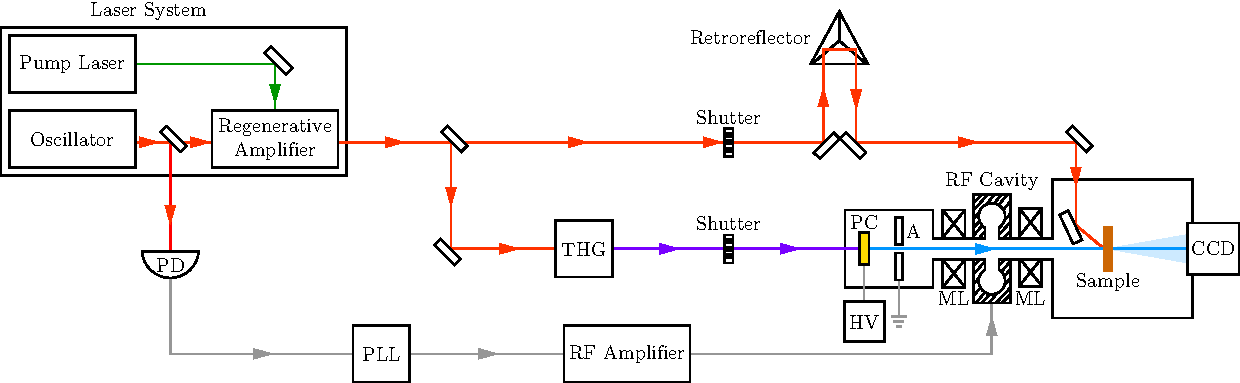
\includegraphics[width = \textwidth]{Figures/fig_ch2_setup-UED.pdf}
  \caption[Schematic of the experimental setup for UED.]{
    Schematic of the experimental setup for UED.
    For simplicity, it is not drawn to scale and minor components are not shown here.
    The black directional lines represent the paths of the electrical signals for
    synchronization, the blue one for the beam path of the electron pulses,
    the others are optical beam paths and their colour indicates the wavelength
    (green = 527 nm, red = 800 nm, and violet = 267 nm).
    Abbreviations: THG = third harmonic generation, PC = photocathode,
    A = anode, HV = high-voltage power supply, ML = magnetic lens, CCD = charge-coupled device,
    PD = photodiode, and PLL = phase-locked loop.
  }
  \label{fig: UED-setup}
\end{figure}

The UED experimental setup used in this thesis is depicted schematically
in Fig.~\ref{fig: UED-setup}. It can be divided up into two major segments:
a femtosecond laser system and an electron diffractometer.
The former is a Ti:Sapph laser system that operates on the same
principles as the commercial one used in the TA setup described in Sec.~\ref{sec: TA-setup}.
The latter is composed of an ultrabright DC-accelerated photoelectron source,
a RF pulse compression system, and a large vacuum sample chamber ($< 10^{-5}$~Pa air pressure)
with a sample holder and CCD~camera (Spectral Instrument~800) for imaging.

In a typical experiment, a Coherent Micra-5 laser acts as the oscillator,
producing a 800-nm, 75-MHz laser pulse train that is selectively amplified through CPA in
a Ti:Sapph REGEN pumped by a Q-switched Nd:YLF laser. The output pulses have a centre wavelength of 800~nm,
a pulse duration of 50~fs, a pulse energy of 0.5~mJ, and a repetition rate that can be
adjusted electronically from 10~Hz to 1~kHz. This light is split into the two beams, one for
pumping the sample and the other for generating the ultrafast electron probe pulses.
The pump beam is first time-delayed using a retroreflector mounted on a motorized translation stage,
focused, and then sent through a viewport of the sample chamber for photoexcitation of the sample.
Simultaneously, the probe beam is frequency-tripled to 267 nm through third harmonic generation%
\footnote{THG is a nonlinear optical process that triples the frequency of an input laser beam.
Here, it is achieved by first frequency-doubling the 800-nm input beam through SHG in a BBO~crystal,
temporally overlapping the 400-nm and remaining 800-nm light using a birefrigent calcite crystal,
and then combining them into 267-nm photons in another BBO~crystal
through sum frequency generation~(SFG).} (THG)
and focused onto a gold photocathode, from which electron pulses are emitted via the photoelectric effect%
\footnote{The photocathode in this setup is a 1-mm thick sapphire substrate with
20~nm of vapour-deposited gold,
which has a work function of ca.~3.8--4.3~eV~\cite{Tsang1991, Aidelsburger2010}.
considering the photon energy of the UV pulse, electrons would be emitted with excess kinetic energy
that translates to significant momentum spread.} with the same temporal profile.
The pulse energy of this UV laser beam is adjusted to be above
the saturation threshold (ca.~$110$ nJ, see Fig.~\ref{fig: electron-char1}a), ensuring that
laser power instability does not lead to fluctuation in the number of electrons per pulse.
%
\begin{figure}[t!]
 \centering
 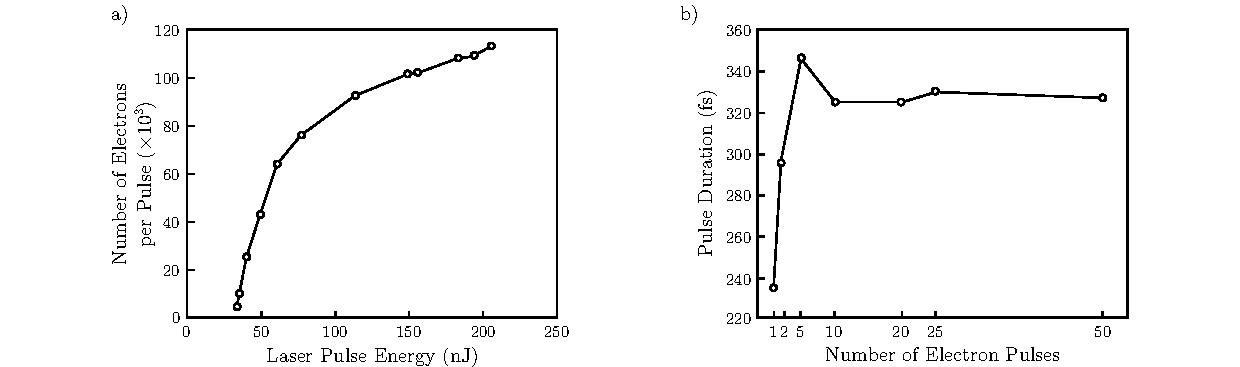
\includegraphics[width = \textwidth]{Figures/fig_ch2_electron-char1.pdf}
 \caption[Plots that illustrate some of the characteristics of the UED electron pulse.]{
   (a) The number of electrons emitted by the photocathode, as inferred by CCD counts,
   has a nonlinear dependence on the energy of the 267-nm laser pulse,
   hence a diminishing return above the saturation threshold.
   (b) Due to pulse-to-pulse variations in the arrival time of the electron pulses,
   the effective pulse duration increases and plateaus as a function of the number over
   which integration occurs.
   Adapted from Ref.~\cite{Yifeng-thesis} with permission of Dr.~Yifeng Jiang.
 }
 \label{fig: electron-char1}
\end{figure}
%
These electrons are accelerated over a distance of ca.~1~cm,
away from the photocathode (held at a potential of $-95$~kV by a high-voltage power supply)
and through a 200-$\unslant\mu$m pinhole%
\footnote{The pinhole blocks electrons that were generated with high transverse momentum;
its diameter can be increased to exchange better transverse beam coherence for higher beam brightness,
or vice versa.} in the anode (held at ground).
A magnetic lens collimates and directs them into a 3-GHz RF cavity.
Here, a time-varying electric field slows down the faster electrons at the front of the pulse and
speeds up the slower ones lagging behind,
thus longitudinally recompressing the pulses that have broadened substantially
due to Coulombic repulsion~\cite{Siwick2002}. As seen in Fig.~\ref{fig: RF-compression},
optimal compression is achieved by synchronizing the zero-crossing of the RF field
with the center of the electron pulses using a timing signal from the oscillator of the laser system;
phase stability is ensured through the use of phase-locked loop
synchronization electronics~\cite{Kiewiet2002}.
A second magnetic lens after the RF cavity focuses the electron beam onto the sample,
which is held in place by a custom holder, itself mounted on
a motorized three-axis linear translation and one-axis rotation stage system.
The transmitted electrons are finally detected by an highly sensitive CCD~camera,
wherein the image sensor is cooled to $-20$~$^{\circ}$C for a ultralow readout noise of
ca.~3~counts per pixel and directly coupled to a fiber plate coated in a layer of phosphor that
converts incident electrons into photons (ca.~100 counts per electron per pixel).
A thin layer of aluminium and carbon is also deposited on top of the phosphor
to filter out unwanted photons, such as those from the pump beam not absorbed by the sample.
The number of electron pulses over which the camera accumulates signal depends on
the time resolution needed for the experiment since the pulse-to-pulse timing jitter of
the electrons effectively broadens the pulse duration (see Fig.~\ref{fig: electron-char1}b).
%
\begin{figure}[t!]
  \centering
  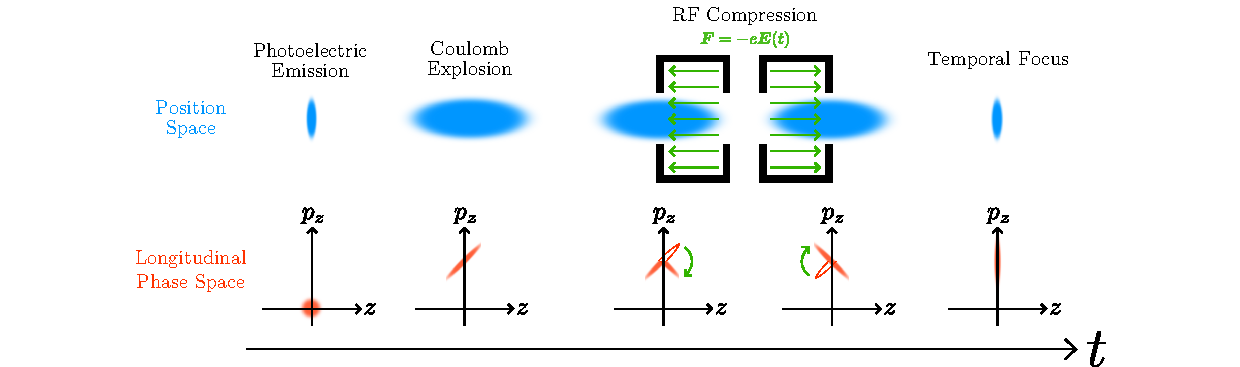
\includegraphics[width = \textwidth]{Figures/fig_ch2_RF-compression.pdf}
  \caption[The principle of RF electron pulse compression.]{
    The principle of RF electron pulse compression. An ultrafast electron pulse is emitted from
    the photocathode via the photoelectric effect and
    is accelerated by the DC electric field between the photocathode and the anode.
    It broadens longitudinally due to Coulombic repulsion and
    a linear velocity chirp develops in phase space as the faster electrons move ahead and
    the slower ones lag behind. During the propagation of the pulse through the RF cavity,
    a precisely synchronized time-varying electric field decelerates the leading electrons
    and accelerates the trailing ones, effectively rotating the electron distribution by
    $-90^{\circ}$ in phase space. Subsequent free-space propagation leads to
    optimal compression of the electron pulse at the sample position.
  }
  \label{fig: RF-compression}
\end{figure}

The electrons generated in this experimental setup have unique characteristics which
make them suitable for ultrafast electron diffraction. They are high energy%
\footnote{The electrons are high energy but not relativistic;
their Lorentz factor $\gamma = 1 + U/E_0$ is less than $2.0$ and
their relativistic beta $\beta = v/c = \sqrt{1 - 1/\gamma^2}$ is only 0.54.} ($95$~keV)
and thus have a de~Broglie wavelength (ca.~$0.038$~\AA) that is two orders shorter
than typical interatomic distances (e.g. $1.54$~\AA~for an average carbon--carbon bond~\cite{CRCBook}).
They are also packed into bunches in great numbers (ca.~$10^{5}$ e$^{-}$ per pulse),
resulting in a beam sufficiently bright to illuminate low-$Z$ materials and
produce high-quality diffraction patterns even at very low repetition rates.
%
A tight focus with a beamwidth of ca.~$200$~$\unslant\mu$m~FWHM at the sample position
is applied to maintain a high enough local transverse coherence width%
\footnote{The local transverse coherence width $L_T^{loc}$ is defined here as
$\hbar/\sigma_{p_x}^{\textrm{loc}}$, where $\sigma_{p_x}^{\textrm{loc}}$ is
the width of the electron momentum distribution in the transverse direction of the beam~\cite{AnnaSipe-thesis}.}
(ca.~$2$~nm, estimated using methods described in Ref.~\cite{Kirchner2013})
for diffraction off of most crystal lattices.
The `camera parameter'%
\footnote{The camera parameter is the conversion factor for the position of diffraction features,
between the camera frame (in pixels) and reciprocal space (in \AA$^{-1}$).
Although determined empirically here, it can be calculated as $4 \unslant[-.2]\pi l / (\lambda L)$,
where $l$ is the camera pixel size ($13.5$~$\unslant\mu$m/px),
$\lambda$ is the electron de~Broglie wavelength ($0.038$~\AA),
and $L$ is the sample-camera distance (ca.~$35$~cm).\label{fn: camera-parameter}}
is determined through calibration with the diffraction pattern of a known sample,
usually single-crystal silicon, and found to be ca.~$1.39 \times 10^{-2}$~\AA$^{-1}$/px.

The duration of the electron pulses is the most important quantity to optimize and
characterize in a UED setup since it strongly affects the ultimate time resolution of
the experiments and depends on a number of experimental parameters.
In the present setup, the pulse duration has been measured for each experiment
using a variety of different techniques. One approach involves measuring
the electron-laser pulse cross correlation~\cite{Siwick2005, Hebeisen2006, Gao2012}
by scattering the electron pulses off the ponderomotive potential generated
by two counter-propagating laser pulses,
a process known as the Kapitza-Dirac effect%
\footnote{Pyotr L. Kapitsa (1894--1984) and Paul A. M. Dirac (1902--1984)
developed the theory of electrons reflected by standing light waves in 1933~\cite{Kapitza1933}.
They were both awarded independently a Nobel Prize in Physics:
Kapitsa in 1978 for his work in low-temperature physics
(along with Arno A. Penzias and Robert W. Wilson
for their discovery of the cosmic microwave background radiation)~\cite{Nobel1971}
and Dirac in 1933 (jointly with Erwin Schr\"{o}dinger)
for a fully relativistic quantum theory~\cite{Nobel1901}.}~\cite{Freimund2001}.
When applied to the current UED setup, this technique yielded an estimate of the pulse duration
in the form of an IRF time of $(430 \pm 75)$~fs~FWHM~\cite{Gao2012}.

\begin{figure}[ht!]
  \centering
  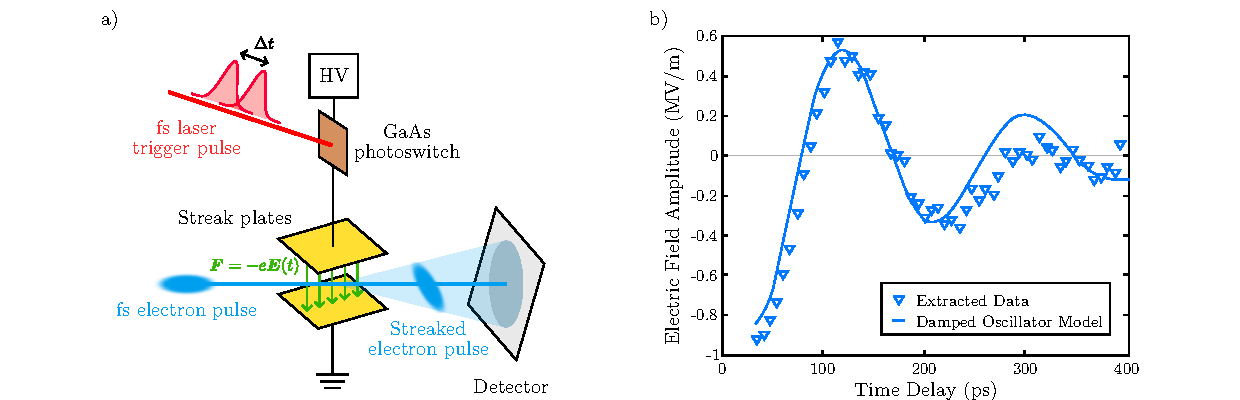
\includegraphics[width = \textwidth]{Figures/fig_ch2_streak-camera.pdf}
  \caption[The principle of electron pulse characterization by streak camera.]{
    The principle of electron pulse characterization by streak camera.
    (a) An ultrafast electron pulse propagating through the gap between the plates of the streak camera
    is deflected transversely by a time-varying electric field triggered by a 800-nm femtosecond laser pulse
    incident on a GaAs photoswitch. The temporal profile of the electron pulse is thus projected
    as the spatial profile of a traverse feature on the camera sensor.
    (b) The electric field between the streak plates oscillates and varies as a function of time delay
    between the trigger laser and the electrons.
    Adapted with permission from Ref.~\cite{Kassier2010}.
  }
  \label{fig: streak-camera}
\end{figure}

Although very precise, the ponderomotive scattering technique is not the one used to
characterize the pulses involved in the work of this thesis.
Here, a compact and convenient device known as a `streak camera',
designed and built by Dr.~G\"{u}nther H. Kassier~\cite{Kassier2010},
is employed to determine the timing of the electron pulses and the associated jitter.
As illustrated in Fig.~\ref{fig: streak-camera}a,
the streak camera can be simply described as a parallel plate capacitor connected
to a pulsed HV~source (${\sim}1500$ V) through a gallium arsenide~(GaAs) wafer
which acts as a photosensitive switch.
A femtosecond laser pulse that is synchronized to the electron pulse illuminates the photoswitch and
triggers an oscillating electric field between the streak plates (see Fig.~\ref{fig: streak-camera}b).
The passing electrons are deflected by this time-varying traverse field and their
longitudinal, temporal profile is projected as a traverse, spatial one.
Optimal streaking is achieved by setting the time delay of the trigger laser pulse such that
the electron pulse propagates through the streak field about its first zero crossing,
taking advantage of the maximum voltage ramp while ensuring zero overall beam deflection.
The pulse duration $\tau_e$ and arrival time $t_e$ of the electrons can be calculated using
the following relations~\cite{Wang2009}:
%
\begin{equation}
\begin{aligned}
    \tau_e & = \frac{\sqrt{ w_\textrm{st}^2 - w_\textrm{un}^2 }}{v_\textrm{st}} \\
    t_e & = \frac{y_\textrm{st} - y_\textrm{un}}{v_\textrm{st}}
\end{aligned}
\end{equation}
%
where $w_\textrm{s}$, $y_\textrm{s}$ are the beamwidth and centre position (in pixels)
of the electron spot on the camera sensor respectively,
given the streak status $s \in \{ \textrm{st: streaked}, \textrm{un: unstreaked} \}$;
$v_\textrm{st}$ is the streak velocity of the streak camera.
The latter is an important parameter to be characterized since it quantifies the time resolution
of the streak camera.
%
\begin{figure}[ht!]
  \centering
  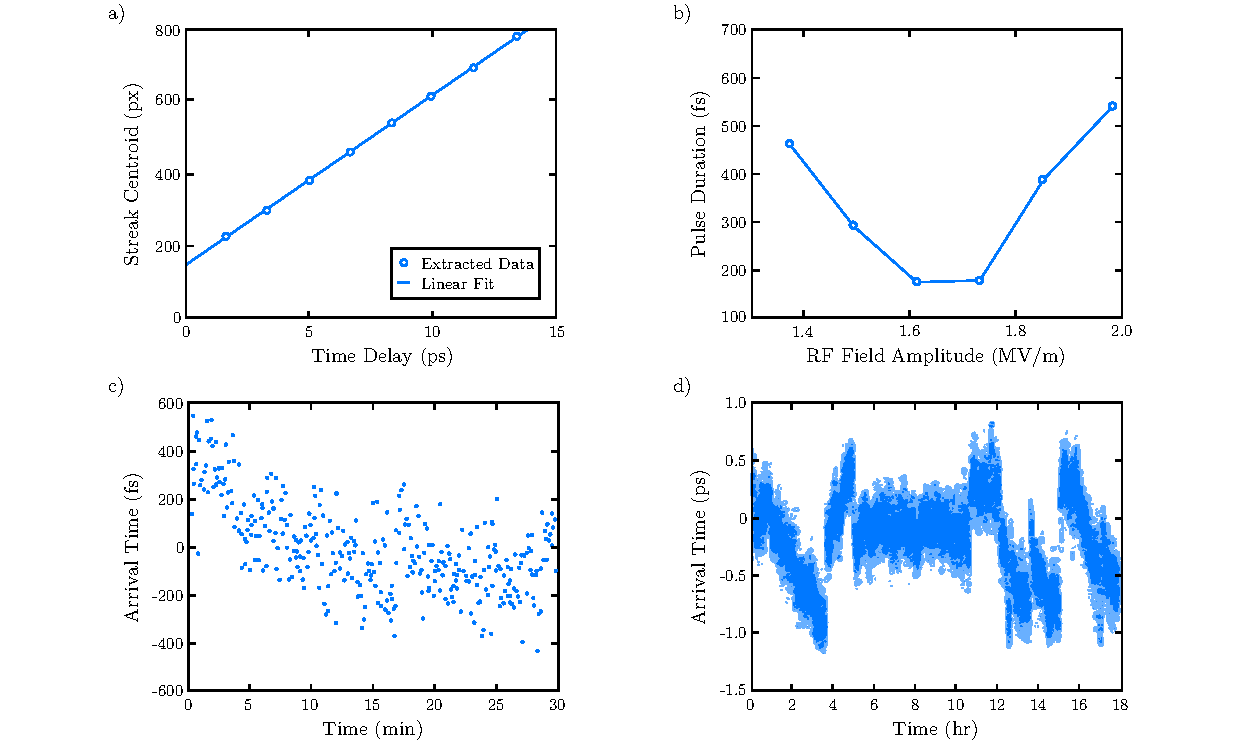
\includegraphics[width = \textwidth]{Figures/fig_ch2_electron-char2.pdf}
  \caption[The streak camera as a UED pulse timing tool.]{
    The streak camera as a UED pulse timing tool.
    (a) Streak velocity~$v_\textrm{st}$ is found as the fitted slope of the deflected position of the
    electrons with respect to the trigger laser time delay.
    (b) Optimal electron pulse compression is achieved by minimizing
    the pulse duration as a function of RF field amplitude.
    (c) Short-time jitter (ca.~$200$~fs~RMS) in the arrival time of the electron pulse.
    (d) Long-time drift in the arrival time monitored over several hours.
    Panel~a is adapted with permission from Ref.~\cite{Jiang2013} while
    Panels~b--f is from Ref.~\cite{Yifeng-thesis} with permission of Dr.~Yifeng Jiang.
  }
  \label{fig: electron-char2}
\end{figure}

In Fig.~\ref{fig: electron-char2}a,
$v_\textrm{st}$ is determined by varying the delay between the arrival time of the
trigger laser and the electron pulse and linearly fitting the centroid of the electron spot
as a function of time delay around the first zero crossing.
Here, it is found to be $(47.2 \pm 0.3)$ px/ps,%
\footnote{Considering the camera pixel size and sample-camera distance
(see Fn.~\ref{fn: camera-parameter}), this translates to a deflection velocity of ca.~$2.8$~mrad/ps.}
fast enough to allow for the single-pulse characterization of the timing of the electrons.
%
In Fig.~\ref{fig: electron-char2}b, the streak camera is used to measure
the single-shot pulse duration as a function of the RF field amplitude involved in electron pulse compression;
this is a key step in the preparation for UED data collection since this measurement is necessary
to determine the optimal field amplitude for maximum pulse compression ($< 200$ fs).
Furthermore, as seen in Fig.~\ref{fig: electron-char2}c and Fig.~\ref{fig: electron-char2}d,
short-time jitter and long-time drift of the arrival time of the electron pulse are monitored and
kept within 500~fs of the target time delay through adjustments of the phase of the RF field.

\begin{figure}[ht!]
  \centering
  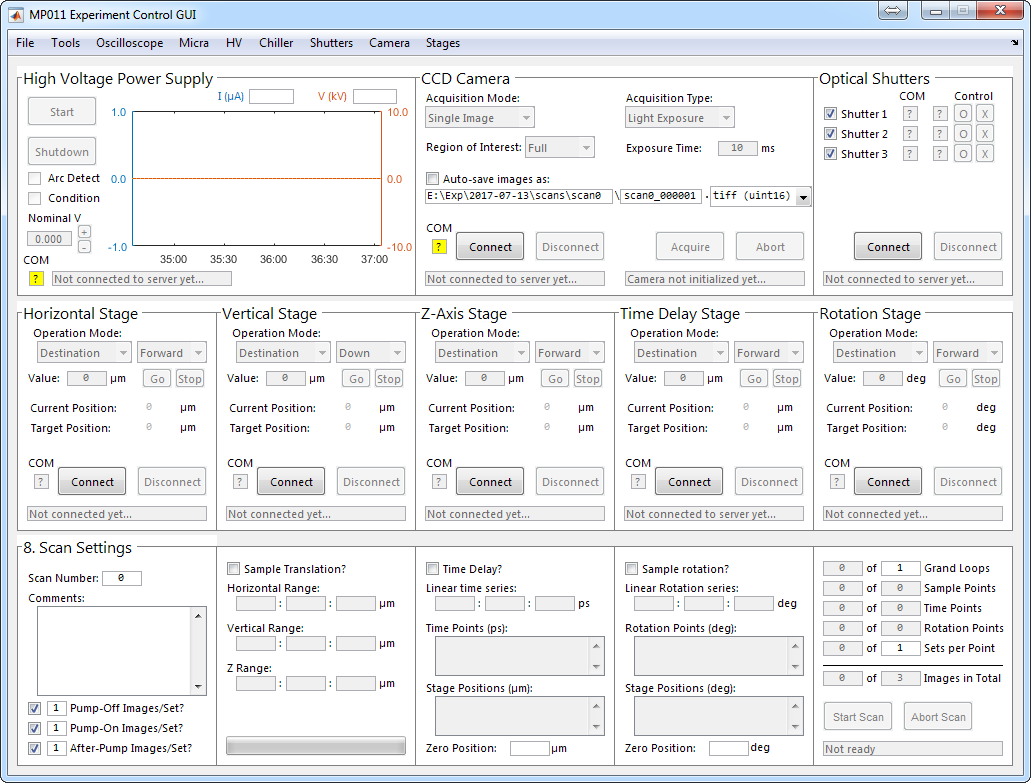
\includegraphics[width = \textwidth]{Figures/fig_ch2_MP011-app.png}
  \caption{
    Screenshot of the graphical user interface of the instrument control and data acquisition application
    that was built for the current UED experimental setup.
  }
  \label{fig: MP011-app}
\end{figure}
%
Beyond the ultrafast laser system and the electron diffractometer,
another key component of the UED setup is the computer program that
enables users to control the different instruments and acquire data.
Here, a full featured application software was developed from scratch
in the \textsc{MATLAB}~R2017b computing environment for this purpose.

Through the graphical user interface (shown in Fig.~\ref{fig: MP011-app}),
it is designed to send commands to and receive data from multiple instruments
hosted on computers connected in a distributed Ethernet network.
A purpose-built C++ server program running on the host computers translates
the TCP/IP packets sent by the control app to serial RS232 signals expected by
the instrument controller, and vice versa. A diagram of the architecture
is shown in Fig.~\ref{fig: MP011-net}.
This design is efficient
since interface- and device-specific functions are abstracted away into their respective applications,
modular since new instruments and users can be added and old ones removed
by simply creating new instances of the server and control apps,
and finally platform-independent since the chosen programming languages and communication protocols
are readily compatible to any modern operating system.
As such, this instrument control paradigm has superseded and replaced
an older, now obsolete scheme that was built using Visual Basic~6.0
as part of the doctoral work of Drs.~Maher Harb~\cite{Maher-thesis} and Meng Gao~\cite{Ray-thesis}.
%
\begin{figure}[ht!]
  \centering
  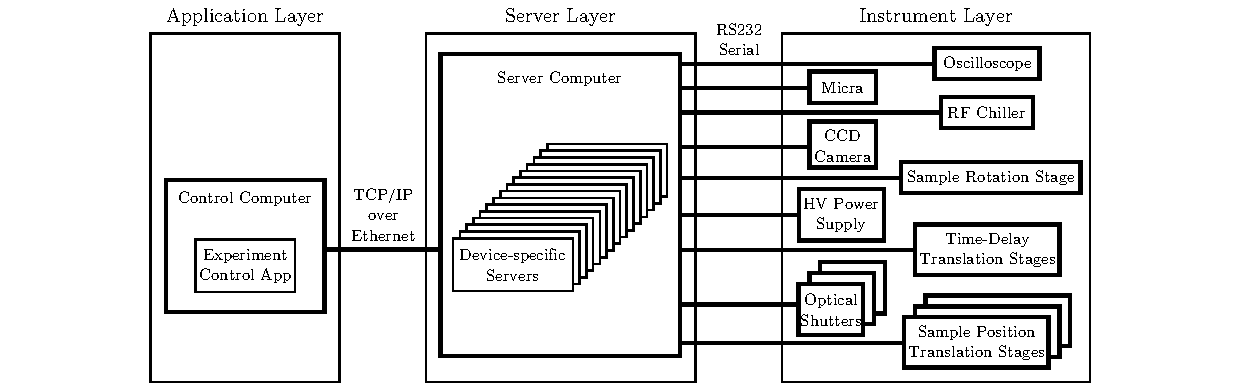
\includegraphics[width = \textwidth]{Figures/fig_ch2_MP011-net.pdf}
  \caption{
    Architecture of the software-hardware interface for instrument control and data acquisition.
  }
  \label{fig: MP011-net}
\end{figure}


%%%%%%%%%%%%%%%%%%%%%%%%%%%%%%%%%%%%%%%%%%%%%%%%%%%%%%%%%%%%%%%%%%%%%%%%%%%%%%%%%%%%

\subsection{Data Analysis --- Part 1}
\label{sec: UED-data-analysis-1}

Analysis of UED data is non-trivial.
%
Given that UED is a time-resolved pump-probe technique,
its data is inherently multidimensional, as in the case of of TA spectroscopy
(see Sec.~\ref{sec: TA-overview}).
A UED data `scan' is collected by scanning over a range of time delay
between the pump and probe pulses and,
for each time point, sets of electron diffraction patterns with alternating pump-shutter states
(`pump-on' and `pump-off') are recorded as high-resolution images.
These scans are then repeated as needed to improve the signal-to-noise ratio
and validate experimental conditions such as the pump laser fluence and sample temperature.
%
As a result, a typical experiment generates a large amount of data
in the form of hundreds of thousands of grayscale images,%
\footnote{
The images can be as large as the CCD~sensor of the camera ($2048 \times 2048$~pixels)
and they are stored as an uncompressed TIFF (`tagged image file format') 6.0 file;
the pixel values are unsigned 16-bit integers.}
%
each of which can be up to $8.4$~MB in size.
%
Hence, analysis of such a dataset --- maybe multi-terabytes in size ---
cannot follow the simplistic, ad hoc process of inspecting each image individually
for time-dependent features.
%
Instead, a `big data' approach%
\footnote{`Big data' herein refers to datasets that are too large to
fit entirely in the random-access memory of a typical personal computer (ca.~$8$~GB).}
to analytics is taken in the UED works presented in this thesis:
first preprocess and reduce, then model and interpret.

\begin{figure}[ht!]
  \centering
  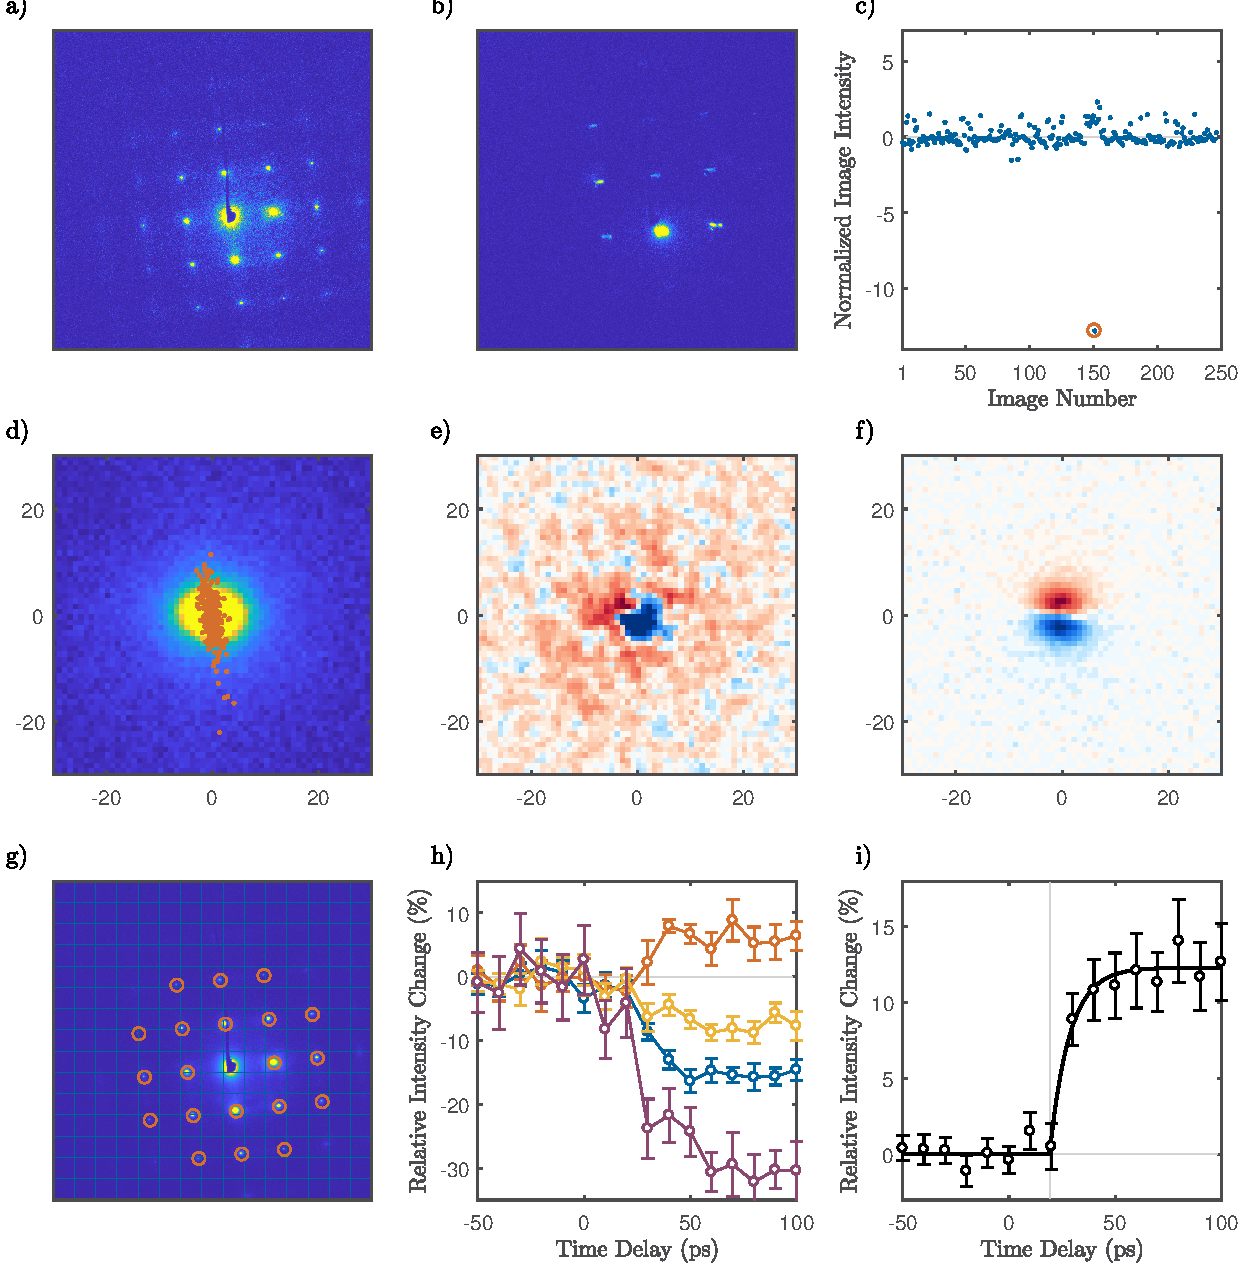
\includegraphics[width = \textwidth]{Figures/fig_UED_preprocess.pdf}
  \caption[Data preprocessing for a single UED scan.]{
  Data preprocessing for a single UED scan.
  Images need to be classified as either (a) nominal or (b) anomalous
  by calculating (c) the total image intensity and cleansing the outliers.
  (d) Beam-pointing instability (exaggerated by five times for clarity)
  is corrected by (g) finding all the visible diffraction spots,
  and using them as targets for motion tracking.
  For comparison, (e) the difference intensity distribution of (d) caused by photoexcitation
  is shown on the same colour scale with
  (f) that which results from a simulated subpixel vertical misalignment ($\delta q = 0.1$~px).
  (h) The image intensity at each visible diffraction spot is integrated and time traces $\Delta I(t)$
  are calculated; traces with $\text{SNR} > 1.5$ are accumulated and (i) fitted to
  a phenomenological signal function to determine $t_0$ of the scan.
  }
  \label{fig: UED-preprocess}
\end{figure}

% Find and reject bad images caused by arcs
Data preprocessing starts by cleansing the dataset of unreliable entries.
%
By inspection, there are obviously nominal and anomalous images,
e.g. Fig.~\ref{fig: UED-preprocess}a and b respectively.
%
The latter are those images acquired usually during anomalous exposure conditions,
caused by electrical discharge and arcing within the electron source assembly,
leading to sudden and large deviations in the electron beam brightness and energy.
These images need to be excluded to prevent the associated intensity variations
from obscuring the subtle changes induced by atomic motions.
%
Here, they are found and flagged by computing a normalized total intensity of every image
and discriminating any outliers from normal system noise.
Normalization of the intensity values is achieved by
subtracting a fitted smoothing spline as proxy for slow, unrelated fluctuations;
`outlier' refers to those data points
that are several standard deviations away from the median.
This process is showcased in Fig.~\ref{fig: UED-preprocess}c,
where the normalized intensity for the images of a sample UED scan is plotted
in multiples of standard deviation.

% Correct for drift caused by beam-pointing instability
Another source of noise that needs to be suppressed is the beam-pointing instability
of the laser beam that generates the UED electrons.
%
Since angular variation in the beam direction translates into
positional drift of the entire diffraction pattern,
pointing fluctuation that occurs between the acquisition of the pump-on and pump-off images
can conjure up changes in intensity that are unrelated to any photoinduced process.
%
Assuming a diffraction spot that is Gaussian in profile,
$I(\boldsymbol{q}) \propto \text{e}^{-\frac{1}{2}q^2 / \sigma^2}$,
and is displaced by some $\delta q \ll \sigma$,
the resulting relative change in intensity can be estimated by
%
\begin{equation}
  \begin{aligned}
      \max\limits_{\boldsymbol{q}}
        & \left\lvert \frac{I(\boldsymbol{q} - \delta \boldsymbol{q}) - I(\boldsymbol{q})}{I(\boldsymbol{q})} \right\rvert
        & \approx \frac{\delta q}{\sigma}
  \end{aligned}
\end{equation}
%
where the maxima are found at $q \pm \sigma$ along $\delta \boldsymbol{q}$.
%
For the diffraction spot displayed in Fig.~\ref{fig: UED-preprocess}d,
with~$\sigma = 4.4$~px, a subpixel displacement~($\delta q = 0.1$~px) introduces
a false signal~($\delta q/\sigma \approx 2.3$~\%)
comparable in magnitude to the real one~($|\Delta I/I_\text{off}| \approx 9.4$~\%),
hence the need for this data-preprocessing step.
%
Most of this problem is already mitigated through the use of an active pointing-stabilization mechanism%
\footnote{
A program authored by Dr.~Meng Gao actively monitors the pointing of the laser
by imaging a beam spot using a high-speed camera (PointGrey Firefly);
it then compensates for any significant deviation in spot position
by controlling a pair of in-beam mirrors mounted on piezoelectric actuators~\cite{Ray-thesis}.
}
that is setup along the optical beam path, immediately after the output of the laser system
(see Fig.~\ref{fig: UED-setup}).
%
However, this optomechanical solution is not perfect and
there are still significant shot-to-shot fluctuations in beam-pointing,
as seen in the positional jitter (ca.~$\pm 0.59$~px) shown in Fig.~\ref{fig: UED-preprocess}d.
%
To eliminate this leftover motion and further improve the SNR of the diffraction data,
some corrective techniques such as video stabilization are borrowed
from the field of computer vision.
%
First, the spots of the diffraction pattern are chosen as the targets for motion tracking.
These are automatically located within each image by first partitioning its area
into a regular array with a spacing less than the minimum inter-spot distance to ensure no concurrency
and then detecting features within each smaller area using image statistics.
A spot is deemed `present' if there is a pixel whose intensity value is the local maximum
and is greater than the local median by multiples (ca.~$30$) of the local standard deviation.
The centre position of the spot $\boldsymbol{q}_0$ is found by fitting
the intensity distribution of `spotty' areas to a general bivariate Gaussian function
%
\begin{equation}
  \begin{aligned}
      I(q_x, q_y)
        & = A \text{e}^{-\frac{1}{2}\left\lvert \mathbf{R} \left( \boldsymbol{q} - \boldsymbol{q}_0 \right)/\mathbf{\Sigma} \right\rvert^2} + B
  \end{aligned}
  \label{eq: gaussian-spot}
\end{equation}
%
where $\mathbf{R} = \mathbf{R}(\theta)$ is just the standard rotation matrix in two dimensions,
$\Sigma_{ij} = \sigma_i \delta_{ij}$, and
the set of fitting parameters is $\{ A, q_{0x}, \sigma_x, q_{0y}, \sigma_y, \theta, B \}$.
%
Fitted centre positions that are outside of the image area are discarded;
those that are closer together than half of the image partition width
are the result of overfitting near single spots and the redundant ones are also discarded.
%
Thus, all the searchable diffraction spots are found and their position is fixed over
every image of a scan.
%
The motion of each image is tracked and stabilized
by calculating the displacement of the centroid of its spot position from a reference point
and using this displacement vector to apply an image translation.
Translation by fractional pixel values is achieved by using a bilinear interpolation
of the image intensity values to calculate values at the translated pixel positions.
The result is a data scan wherein any photoinduced changes in diffraction features
can be directly and readily discerned from background noise (Fig.~\ref{fig: UED-preprocess}e).

Occasionally, a data scan would fail to exhibit any signal --- sigmoid-like changes in intensity
over time delay --- at any diffraction spot despite beam-pointing stabilization.
Such empty scans can be caused by a variety of experimental issues: a lack in spatial or temporal overlap
between the pump laser and the probe electron pulses, overly noisy pump and probe sources,
and sample degradation.
They need to be found and excluded from further analysis
to prevent SNR~loss when the entire dataset is ultimately averaged together.
%
This is achieved by first integrating the image intensity in each diffraction spot
and calculating their individual time trace~$\Delta I(t) = \frac{I_\text{on}(t) - I_\text{off}}{I_\text{off}}$
(Fig.~\ref{fig: UED-preprocess}h).
Traces whose values at $t \gg 0$ are statistically different from
those at $t \ll 0$ are averaged together to produce an overall time trace.
As in Fig.~\ref{fig: UED-preprocess}i,
signal is deemed to be present in a scan if its overall trace fits reasonably to
a Gaussian error function of the form $A \: \text{erf}\left(\frac{t-t_0}{\tau}\right) + B$,
where $t_0$ is the time-zero of the scan.

UED signals are not necessarily only found in the immediate area at and around the visible spots
of a diffraction pattern. Symmetry in a crystal structure causes `systematic absence'
or complete extinction of intensity of certain diffraction spots;
photoinduced structural dynamics can break such crystallographic symmetries
and scatter intensity into reciprocal lattice points
that were previously empty~\cite{Brefuel2009, Eichberger2010}.
%
A region-of-interest (ROI) search, more advanced than the earlier spot location analysis,
is thus performed to find and index the reciprocal lattice of the diffraction pattern.

To start, the beampointing-stabilized images are averaged to produce a reference image
to reduce shot noise. Further noise removal is done by applying
a two-dimensional adaptive Wiener filter%
\footnote{First proposed in 1949 by Norbert Wiener (1894--1964),
this image processing technique estimates the local mean and variance around each pixel
and then applies more or less smoothing in response~\cite{Lim1990}.} to the image.
%
Then, a mask is produced to specify areas of the UED image which are devoid of useful information
and need to be excluded from further analysis.
These include pixels that have been saturated, damaged, or shaded by a beam block.
Given that they are delimited by sharp intensity gradients, a Canny edge detector%
\footnote{This computational technique was developed by John F. Canny (1958--present) in 1986;
it detect edges by searching for connected pixels whose gradient magnitude is
between two given thresholds~\cite{Canny1986}.}
is used to trace their outline; a flood-fill pixel operation finds and fills the `holes'~\cite{Soille2004}.
In Fig.~\ref{fig: UED-rlattice}a, the outline of the beam block thus found is shown as a green line.

\begin{figure}[t!]
  \centering
  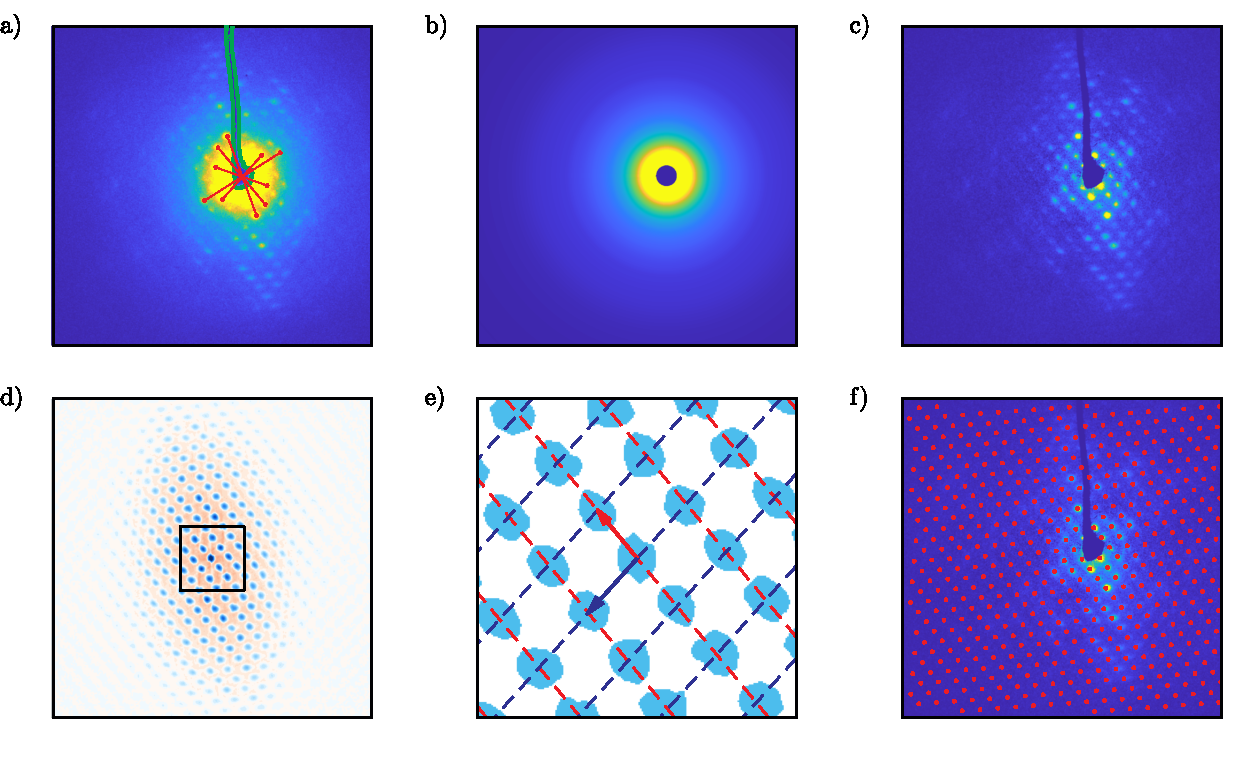
\includegraphics[width = \textwidth]{Figures/fig_UED_rlattice.pdf}
  \caption[Illustration of the steps of ROI search in a UED image.]{
  Illustration of the steps of ROI search in a UED image.
  %
  Step 1: construct a mask of any beam block by tracing its outline (green) with a Canny edge detector
  and determine the centre of the diffraction pattern from Friedel pairs (red).
  Step 2: estimate the intensity distribution of the transmitted beam (b)
  and subtract it from (a) to obtained a background-free image (c).
  Step 3: calculate the Laplacian of the autocorrelation of the image (d)
  and vectorize the centroid position of all the labeled connected regions (e).
  Step 4: position all the ROIs of the UED image (f)
  by generating a spanning grid from the lattice vectors found in (e).
  }
  \label{fig: UED-rlattice}
\end{figure}

To anchor the ROI search, the centre of the diffraction pattern needs to be found.
A rough estimate of its position is obtained by calculating the `centre of intensity' or
intensity-weighted arithmetic mean of the position of $>100$~random points
uniformly distributed over the masked image;
this is used to match diffraction spots into Friedel pairs%
\footnote{Named after Georges Friedel (1865--1933),
these pairs are the diffraction spots with Miller index $(h, k, l)$ and
$(\bar{h}, \bar{k}, \bar{l} )$~\cite{XRDBook}.}
amongst those found earlier.
By averaging the midpoint of the lines connecting these pairs of points,
a more accurate position of the centre is obtained.

With the centre of intensity found, subtraction of the background centered at $(000)$ can proceed
to enhance the intensity contrast between the diffraction spots and the transmitted beam.
%
Several techniques are known for performing this task
from literature (see Ref.~\cite{Downing2001} and the references therein);
however, they were found to be either ill-suited for automation or computationally labourious.
%
Here, given the isotropy of this intensity distribution, a coordinate transformation is applied
to the masked image that converts the Cartesian coordinates of its pixels to a set of polar ones
relative to the centre position. The pixels are then sorted in increasing order and
binned by their radial coordinate, rounded to the nearest integer.
The minimum intensity value within each bin is now taken to be the value of the background
at the prerequisite distance from the centre
as a mean to minimize the intensity contribution of the diffraction spots.
A background image (Fig.~\ref{fig: UED-rlattice}b) is reconstructed from this radial trace
by applying the reverse coordinate transformation and
using spline interpolation for non-integer radius values.
%
Hence, the background-free image (Fig.~\ref{fig: UED-rlattice}c) can be obtained
from the masked image (Fig.~\ref{fig: UED-rlattice}a).
%
Note that, in cases where the crystallinity of the sample and the quality of the electron beam
are poor, the diffraction spots can become so broad as to interfere
with the background subtraction algorithm, leaving faint ring-like artifacts.
%
Non-radial components of the background --- contributed by diffuse scattering due to crystal disorder ---
are left untreated here and may be dealt with using either a Fourier high-pass spatial filter
or an iterative model-based approach as described in Ref.~\cite{Grigorieff1995}.

Despite the preliminary noise removal and $(000)$-beam subtraction,
the ROI search is not performed directly on the background-free image.
As seen in Fig.~\ref{fig: plotDiffInt}, the diffraction pattern intensity
is effectively a periodic function $|S(\boldsymbol{q})|^2$ modulated by
a structural term $I_\text{st}(\boldsymbol{q})$.
The uneven modulation can result in the effective intensity extinction of low-order diffraction spots,
precluding a direct evaluation of the periodicity and indexing of the ROIs.
Here, this problem is solved by performing the ROI search instead on
a derived quantity $C(\boldsymbol{q}) = \nabla^2 \left( I(\boldsymbol{q}) \ast I(\boldsymbol{q}) \right)$,
where the convolution can be replaced by a sequence of fast Fourier transforms,
$I(\boldsymbol{q}) \ast I(\boldsymbol{q}) =
\mathcal{F}^{-1}\{ \mathcal{F}\{I(\boldsymbol{q})\}^2\}$.
%
Amongst the values of $C(\boldsymbol{q})$, the ROIs are now clearly visible
as a regular array of negative regions (Fig.~\ref{fig: UED-rlattice}e)
which are localized by masking all the positive regions, flattening the negative ones,
and applying `connected-component labeling'%
\footnote{This is performed using the \texttt{regionprops} function
in \textsc{MATLAB}~R2017b.} to the binary image.
%
Once labeled, the centroid of each array object is calculated and
the relative positions of the two non-collinear objects nearest to the image centre
can be used to define the two basis vectors necessary to index and specify
the position of every possible ROI within the diffraction pattern (Fig.~\ref{fig: UED-rlattice}f).

By integrating the intensity in the circular region centered at the positions found earlier,
the stack of pump-probe UED images of a data scan is reduced to a set of time traces.
Before the traces of multiple scans can be combined, their `clocks' need to be synchronized.
%
Significant drifts in the baseline arrival time of the probe pulse relative to that of the pump pulse
can occur as a result of scan-to-scan variation in environmental conditions,
which affects the timing electronics of the RF pulse compression system (Fig.~\ref{fig: UED-temp-vs-streak}).

\begin{figure}[t!]
  \centering
  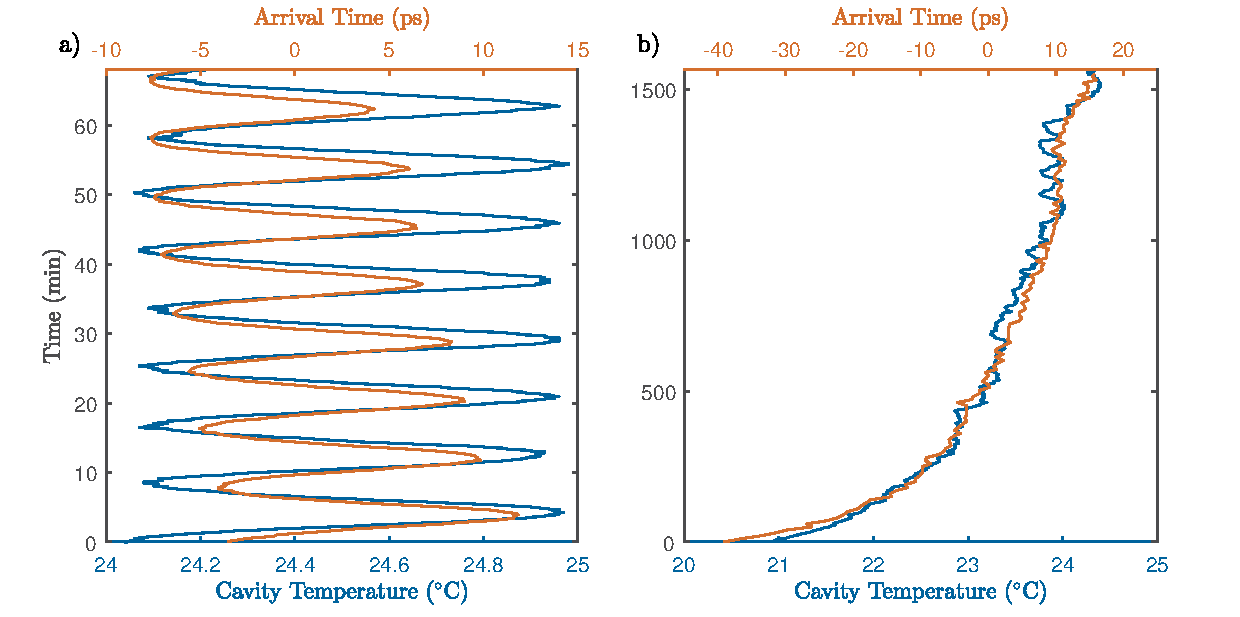
\includegraphics[width = \textwidth]{Figures/fig_UED_tempvsstreak.pdf}
  \caption[Correlation between the temperature of the RF cavity in the UED setup and
  the arrival time of the electron pulses under different conditions.]{
    Correlation between the temperature of the RF cavity in the UED setup and
    the arrival time of the electron pulses under different conditions.
    (a) The parameters of the proportional-integral-derivative~(PID) temperature controller
    for the RF cavity were intentionally detuned to generate oscillations.
    (b) Values were measured in the midst of the thermal equilibration of the UED setup.
  }
  \label{fig: UED-temp-vs-streak}
\end{figure}

To mitigate this issue, the time delay of each scan is shifted by the time-zero $t_0$
fitted during the data preprocessing step (Fig.~\ref{fig: UED-preprocess}i),
enabling the compilation of time traces measured
during different sessions of data collection (Fig.~\ref{fig: UED-rebin}a).
%
However, these traces cannot be directly averaged together
since the time points are now misaligned.
The solution is to treat the data like underexposed photographs and
apply an image processing technique known as `histogram equalization'
to enhance contrast by flattening the frequency distribution.
%
\begin{figure}[ht!]
  \centering
  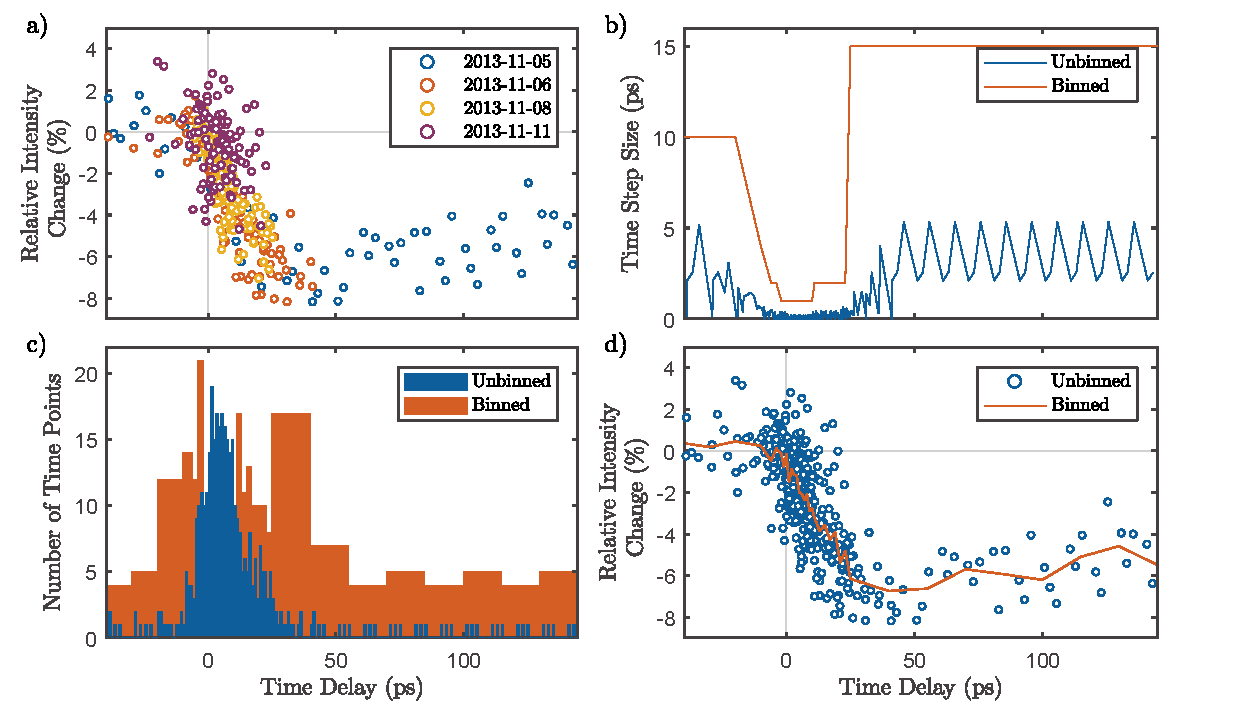
\includegraphics[width = \textwidth]{Figures/fig_UED_rebin.pdf}
  \caption[Combining UED data after time-zero correction with histogram equalization.]{
    Combining UED data after time-zero correction with histogram equalization.
    (a) Time traces from multi-day datasets cannot be directly averaged due to time point misalignment.
    A fix is to selectively choose (b) larger time steps, (c) broaden the sampling histogram.
    By calculating the mean of the data points within the new bins,
    (d) an average time trace can be obtained.
  }
  \label{fig: UED-rebin}
\end{figure}
%
As seen in the temporal sampling histogram (Fig.~\ref{fig: UED-rebin}c),
the distribution of time points is very narrow around the interval around $t = 0$,
i.e.~the temporal contrast of the compiled data is too low.
By choosing a new sampling scheme with selectively larger time steps,
equalization is achieved and a final noise-reducing average can then be taken
via a rebinning of the data point (Fig.~\ref{fig: UED-rebin}d).

%%%%%%%%%%%%%%%%%%%%%%%%%%%%%%%%%%%%%%%%%%%%%%%%%%%%%%%%%%%%%%%%%%%%%%%%%%%%%%%%%%%%

\subsection{Data Analysis --- Part 2}
\label{sec: UED-data-analysis-2}

At this point, further analysis of the UED data would traditionally involve
a mapping from reciprocal to real space by building a structure model.
This model would then be used to refine a set of reaction coordinates against
the diffraction intensities at each time point, thus producing a `molecular movie.'
%
Instead, a recognition could be that UED data
(changes in diffraction intensity $\delta I$ as a function of time $t$ and scattering vector $q$)
is structurally equivalent to TA data (changes in absorbance $\delta A$ as a function of time~$t$ and wavelength~$\lambda$)
and the structural dynamics as observed by UED can be elucidated within reciprocal space directly
through an analysis scheme comparable to that of TA.
%
This insight is grounded beyond the superficial similarity in functional dependence
but deeper in the dimensionality of the measurements.
%
In broadband TA spectroscopy, the number of sampled wavelengths is much greater than
the number of optically active species within the probe volume;
in UED of small molecules,
the number of observable diffraction spots, ca.~$400$, is similarly greater than
the number of degrees of freedom~(DOFs)%
\footnote{For the molecule (EDO-TTF)\textsubscript{2}PF\textsubscript{6},
there are $N = 35$ non-hydrogen atoms in the asymmetric unit, hence $3N-6 = 99$~DOFs.}
in the form of molecular translations, rotations, and vibrations.
In both cases, there is redundant complexity within the datasets that can be reduced
using singular value decomposition~(SVD).

\begin{figure}[t!]
  \centering
  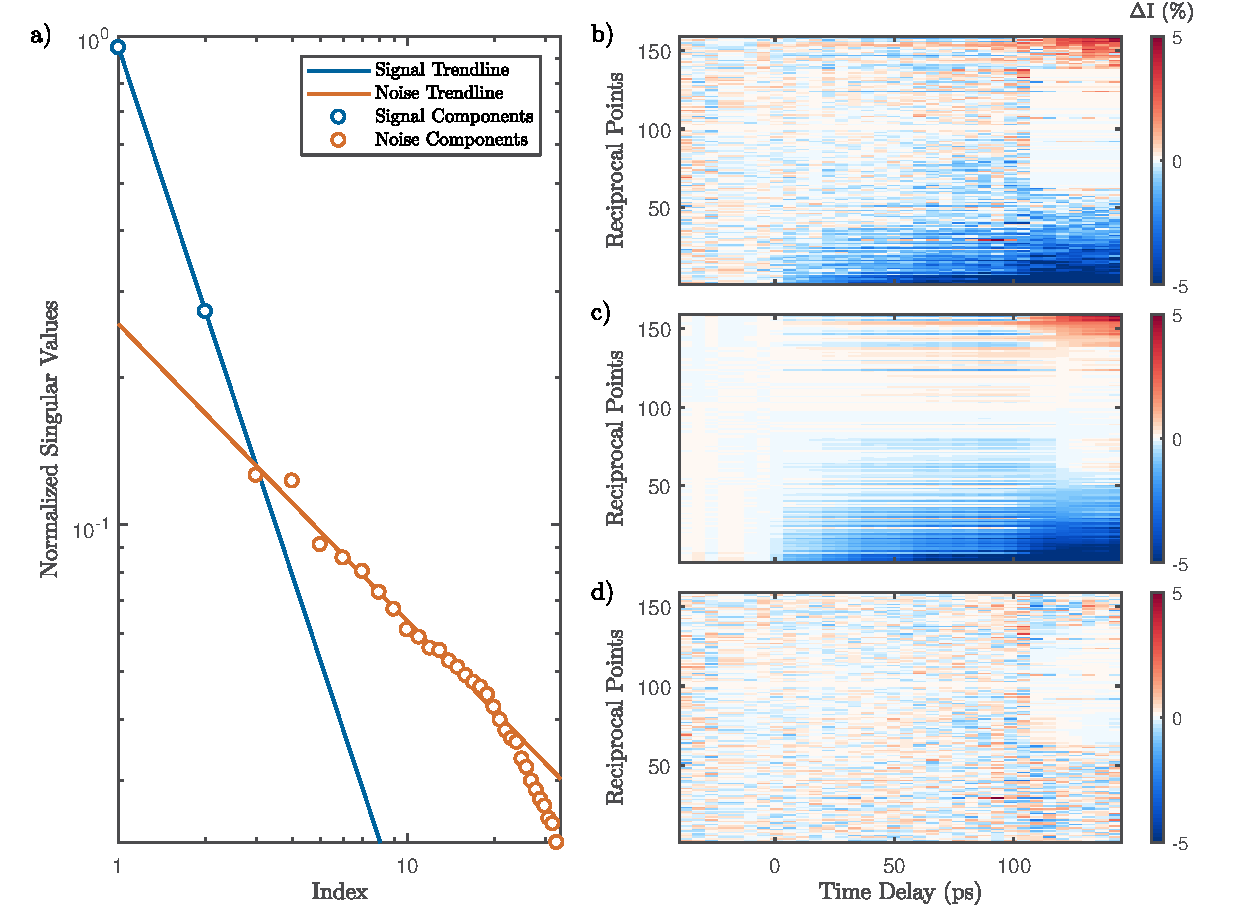
\includegraphics[width = \textwidth]{Figures/fig_UED_svd.pdf}
  \caption[Low-rank approximation of UED data matrix via singular value decomposition and truncation.]{
  Low-rank approximation of UED data matrix via singular value decomposition and truncation:
  (a) a log-log plot of the singular values $s_i$ shows that there are two types of singular components;
  (b) Time-dependent features are clearly present in the original data matrix but are partly obscured by noise;
  (c) summation of the terms before the dividing index $P'$, as per Eq.~\eqref{eq: UED-SVD}, returns a data matrix that is representative of
  the dynamics of interest;
  (d) summing those after yields data that is devoid of anything above SNR.
  }
  \label{fig: UED-svd}
\end{figure}

As in Sec.~\ref{sec: TA-data-analysis} and Fig.~\ref{fig: UED-svd}b, concatenate row-wise
the time trace of all diffraction spots, $\Delta I (t, \boldsymbol{q})$,
into a $M \times N$ data matrix $\mathbf{\Delta I}$,
$M$ and $N$ are the number of diffraction spots and time points respectively,
%
\begin{equation}
  \begin{aligned}
    %t & = \{ t_1, ..., t_N \} \\
    %\lambda & = \{ \lambda_1, ..., \lambda_M \} \\
    \Delta I(t, \boldsymbol{q}) \rightarrow \mathbf{\Delta I} =
    \begin{bmatrix}
        \Delta I(t_1, \boldsymbol{q}_1) & \cdots & \Delta I(t_N, \boldsymbol{q}_1) \\
        \vdots & \ddots & \vdots \\
        \Delta I(t_1, \boldsymbol{q}_M) & \cdots & \Delta I(t_N, \boldsymbol{q}_M)
    \end{bmatrix}
  \end{aligned}
\end{equation}
%
which can be factored via SVD into a linear combination of reciprocal-space and temporal features,
%
\begin{equation}
  \begin{aligned}
    \mathbf{\Delta I} & = \mathbf{U} \mathbf{S} \mathbf{V}^\mathsf{T} \\
      & = \sum_{i = 1}^P s_i \mathbf{u}_i \otimes \mathbf{v}_i^\mathsf{T}
    \label{eq: UED-SVD}
  \end{aligned}
\end{equation}
%
where $\mathbf{U} = \left[ \mathbf{u}_i \ldots \mathbf{u}_M \right]$
and $\mathbf{V} = \left[ \mathbf{v}_j \ldots \mathbf{v}_N \right]$ are orthogonal matrices
whose columns are the left and right singular vectors,
$\mathbf{u}_i = u_i(\boldsymbol{q})$ and $\mathbf{v}_j = v_i(t)$;
$\mathbf{S}$ is the $M \times N$ diagonal matrix of rank $P$ and whose diagonal elements $s_i$,
sorted in descending order, are the singular values of $\mathbf{\Delta I}$.
%
Given that the dynamics in UED data, as in TA~data, are effectively overdetermined,
a `low-rank approximation' of $\mathbf{\Delta I}$ is made
by truncating the sum of singular components $\mathbf{u}_i \otimes \mathbf{v}_i^\mathsf{T}$
at some $P' \ll P$.
As seen in a log-log plot of the singular values (Fig.~\ref{fig: UED-svd}a),
a flexure neatly segregates the major components from minor ones.
Given that the latter appear to be uncorrelated noises by inspection (Fig.~\ref{fig: UED-svd}d),
the penultimate index is chosen to be the value of $P'$,
yielding a data matrix that retains the dynamics of interest (Fig.~\ref{fig: UED-svd}c)
while losing the weakly contributing and undesirable features.

% Global analysis
To complete the global analysis of the UED data in reciprocal space,
a phenomenologically model function $f_i$ is chosen to fit $v_i(t)$,
the time-dependent part of each singular component (Fig.~\ref{fig: UED-svdfit}a).
Here, it is a linear combination of $Q$ exponential decay functions,
convolved with a Gaussian instrument response function
$\textrm{IRF}(t) = \text{e}^{- \frac{1}{2} t^2/\tau_\text{IRF}^2}$,
\begin{equation}
  \begin{aligned}
    f_i(t, \{ b_{i j}\}, \{k_j\})
        & = \sum_{j = 1}^Q b_{i j} \left( H(t) \text{e}^{-k_j t}\right) \ast \text{IRF}(t)
  \end{aligned}
  \label{eq: UED-GA}
\end{equation}
%
where $H(t)$ is the Heaviside function, $\tau_\text{IRF} \approx 180$~fs,
and $\tau_j = 1/k_j$ are the relevant time constants of the dynamics.%
\footnote{For reference,
$ \left( H(t - t_0) \text{e}^{-k t}\right) \ast \text{e}^{- \frac{1}{2} t^2/\tau^2} =
\frac{1}{2} \text{e}^{\frac{1}{2} k^2 \tau^2 - k (t - t_0)}
\left( 1 +
\text{erf}\left( \frac{t - t_0 - k \tau^2}{\sqrt{2} \tau} \right)
\right)$.
} In the case of the data shown in Fig.~\ref{fig: UED-svd},
only three exponential terms are necessary to produce good fits (Fig.~\ref{fig: UED-svdfit}a).
By re-summing the singular components using the fitted $v_i(t)$,
%
\begin{equation}
  \begin{aligned}
    G(t, \boldsymbol{q})
      & = \sum_{i = 1}^{P'} s_i u_i(\boldsymbol{q})
        \left( \sum_{j = 1}^Q b_{i j} \left( H(t) \text{e}^{-k_j t}\right) \ast \text{IRF}(t) \right)
  \end{aligned}
\end{equation}
%
a fit line $G(t, \boldsymbol{q})$ is produced for the time trace of
every sampled reciprocal point (Fig.~\ref{fig: UED-svdfit}b--d).

\begin{figure}[t!]
  \centering
  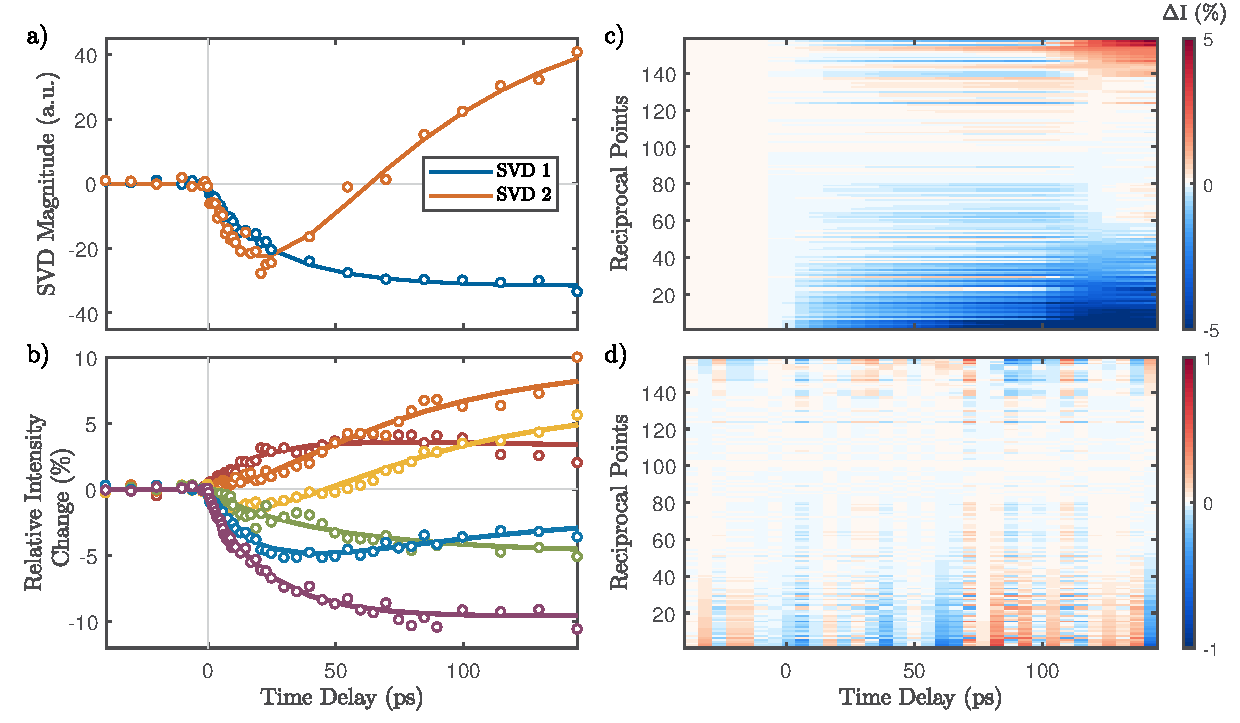
\includegraphics[width = \textwidth]{Figures/fig_UED_svdfit.pdf}
  \caption[Global analysis of UED data.]{
  Global analysis of UED data:
  (a) fitting of the principal right singular vectors $\mathbf{v}_i = v_i(t)$ is achieved
  using a few-parameter exponential model $f_i(t, \{ b_{i j}\}, \{k_j\})$ (see Eq.~\eqref{eq: UED-GA});
  the fitted parameters can then be used to reconstruct a global fit,
  i.e.~fit lines for all time traces;
  data for six select diffraction spots is shown in (b),
  and in (c), for all spots;
  the global residual is shown in (d).
  }
  \label{fig: UED-svdfit}
\end{figure}

% Talk about dimensionality reduction?

Another insightful and independent approach to analyzing UED data within reciprocal space directly
is to compute the Pearson correlation coefficient%
\footnote{Named after English mathematician Karl Pearson (1857--1936)~\cite{KarlPearson}.}
between the measured structure factors of the photoexcited molecule, $F_\text{exc}(t, \boldsymbol{q}_j)$,
with those of a reference, $F_\text{ref}(\boldsymbol{q}_j)$,
%
\begin{equation}
  \begin{aligned}
    P_\text{exc, ref}(t)
      & = \frac{\text{cov}(\zeta_\text{exc}(t, \boldsymbol{q}_j), \zeta_\text{ref}(\boldsymbol{q}_j))}{\sigma_\text{exc} \sigma_\text{ref}}
  \end{aligned}
  \label{eq: UED-Pearson}
\end{equation}
%
where
%
\begin{equation}
  \begin{aligned}
    \zeta_A(\boldsymbol{q}_j) & = \frac{F_A(\boldsymbol{q}_j)}{\bar{F}_A(\boldsymbol{q}_j)} - 1\\
    \text{cov}(\zeta_A, \zeta_B)
      & = \sum_{j = 1}^M \left( \zeta_A(\boldsymbol{q}_j) - \bar{\zeta}_A(\boldsymbol{q}_j) \right)
        \left( \zeta_B(\boldsymbol{q}_j) - \bar{\zeta}_B(\boldsymbol{q}_j) \right) \\
    \sigma_\text{A}
      & = \sqrt{\sum_{j = 1}^M \left(\zeta_A(\boldsymbol{q}_j) - \bar{\zeta}_A(\boldsymbol{q}_j) \right)^2} \\
  \end{aligned}
\end{equation}
%
and $\text{A}, \text{B}$ are the molecular states and
the overline indicates an arithmetic mean.
Given that the set of structure factors in a diffraction pattern is an expression of
the atomic coordinates of the target crystal structure,
the value of $P_\text{A, B}$ --- which varies from $-1$ to $1$ ---
quantifies the similarity between the molecular structure of two states.
In the case of a system with one or more known thermally accessible states $S_n$ beyond
the ground state $S_0$, a semblance of the space of all possible molecular configurations
can be constructed in the form of the Cartesian coordinates
$\left( P_\mathrm{X, S_0}, P_\mathrm{X, S_1}, \ldots, P_\mathrm{X, S_N} \right)$.
By following the time evolution of the point
$\boldsymbol{P}(t) = \left( P_\mathrm{exc, S_0}(t), P_\mathrm{exc, S_1}(t), \ldots,  P_\mathrm{exc, S_N}(t) \right)$,
the trajectory of the excited state through configuration space can be traced out.
This point is illustrated in Fig.~\ref{fig: UED-pearson} using the UED data of
(EDO-TTF)\textsubscript{2}SbF\textsubscript{6}.
%
\begin{figure}[t!]
  \centering
  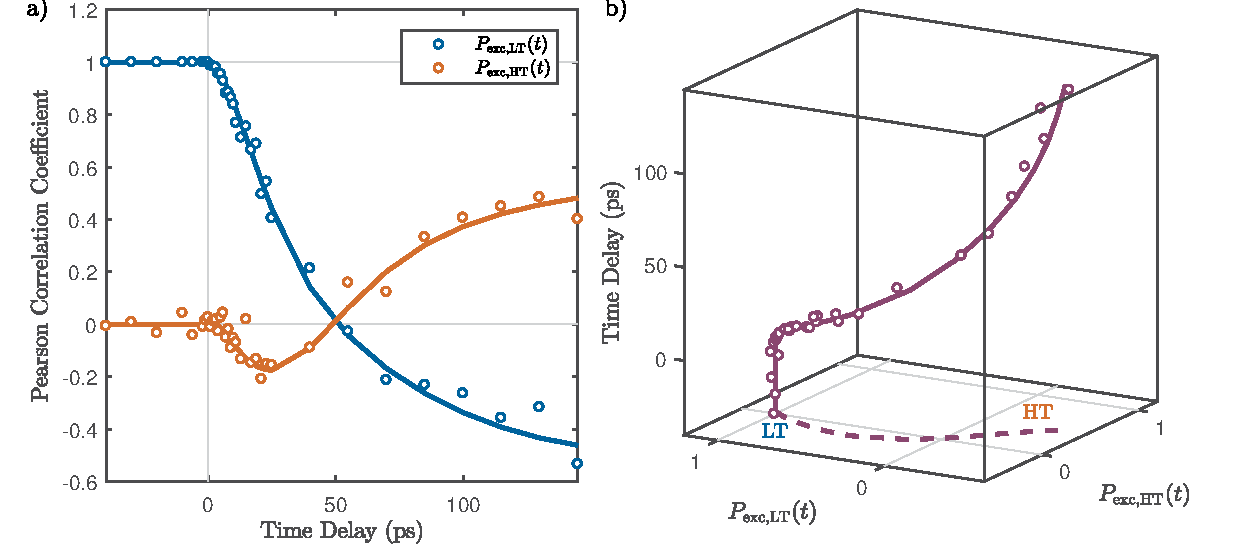
\includegraphics[width = \textwidth]{Figures/fig_UED_pearson.pdf}
  \caption[Pearson correlation analysis of UED data.]{
  Pearson correlation analysis of UED data:
  (a) computing the value of $P_\text{exc, ref}(t)$ for each of the two reference states (LT and HT)
  at each time point $t$ using Eq.~\eqref{eq: UED-Pearson};
  (b) plotting simultaneously the two sets of coefficients, rescaled such that $P_\mathrm{LT, HT}(t) = 0$,
  reveals the configurational pathway taken by the photoexcited molecule as it undergoes relaxation
  from the LT region (blue) to somewhere near the HT region (red).
  Note that these data points are derived from UED measurements made on
  crystals of (EDO-TTF)\textsubscript{2}SbF\textsubscript{6}.
  }
  \label{fig: UED-pearson}
\end{figure}
%
This molecule exists in its ground or `low temperature' (LT) state under normal conditions
undergoes a phase transition to a structurally distinct `high temperature' (HT) state
above 242~K (more details in Sec.~\ref{sec: UED-EDOSbF6}).
By correlating the measured diffraction intensities of the photoexcited state with those
of the LT and HT states, the molecule can be observed in Fig.~\ref{fig: UED-pearson}a
evolving away from its starting LT structure to a final product state structure
that is unexpectedly distinct from the HT structure.

Note that the Pearson correlation analysis requires as input the structure factors
of the photoexcited molecules, $F_\text{exc}(t, \boldsymbol{q}_j)$,
not those measured simply while the laser pump state is `on,' $F_\text{on}(t, \boldsymbol{q}_j)$.
%
To deconvolve these two quantities, it is necessary to make some assumptions about
the spatial distribution of the excited molecules in the crystal
on the microscopic scale~\cite{CoppensBook, Coppens1998, Coppens2005, Reeuwijk2000}.
In the case where strong photoexcitation or photoinduced cooperativity
generate many excited molecules that cluster together into sizable%
\footnote{On the order of the coherence length of the probe electrons} domains,
the structure factors are related by
%
\begin{equation}
  \begin{aligned}
    |F_\text{on}(t, \boldsymbol{q}_j)|^2
      & = \eta_\text{exc} |F_\text{exc}(t, \boldsymbol{q}_j)|^2
        + \left( 1 - \eta_\text{exc} \right) |F_\text{off}(\boldsymbol{q}_j)|^2
  \end{aligned}
\end{equation}
%
In the case of weak photoexcitation, the few excited molecules are randomly distributed
within an unperturbed lattice of ground state molecules,
an expression of the structure factors is instead given by
%
\begin{equation}
  \begin{aligned}
    F_\text{on}(t, \boldsymbol{q}_j)
      & = \eta_\text{exc} F_\text{exc}(t, \boldsymbol{q}_j)
        + \left( 1 - \eta_\text{exc} \right) F_\text{off}(\boldsymbol{q}_j)
  \end{aligned}
  \label{eq: coppens}
\end{equation}
%
where $\eta_\text{exc}$ is the excitation fraction.
Given that UED experiments are performed within a regime where
the fluence of the pump laser is relatively low and the sample response is linear,
the latter case is more likely. The absence of superlattice diffraction spots ---
associated with domain formation --- further suggests that the random-distribution model
is the appropriate choice for the works of this thesis.

Notice that $\eta_\text{exc}$ is still unknown and
one way to determine its value is using the crystallographic information and
the excitation conditions of the sample,
%
\begin{equation}
  \begin{aligned}
    \eta_\text{exc} = \frac{N_\text{exc}}{N_\text{tot}}
  \end{aligned}
  \label{eq: nexc-optical}
\end{equation}
%
The numerator $N_\text{exc}$ is the number of absorbed pump-laser photons that lead to photoexcitation,
%
\begin{equation}
  \begin{aligned}
    N_\text{exc}
      & = \left( \frac{E_\text{pump}}{h c / \lambda_\text{pump}} \right)
        \Phi \left( 1 - 10^{-A}\right) \text{erf}\!\left( \frac{w_\text{probe}}{\sqrt{2} w_\text{pump}}\right)
  \end{aligned}
\end{equation}
%
where $E_\text{pump}, \lambda_\text{pump}, w_\text{pump}$ are
the pulse energy, wavelength, and beamwidth of the pump laser,
$w_\text{probe}$ is the beamwidth of the probe electrons, and
$\Phi, A$ are the quantum yield and absorbance of the targeted transition;
the denominator $N_\text{tot}$ is the total number of absorbers
within the excitation volume of the pump laser,
%
\begin{equation}
  \begin{aligned}
    N_\text{tot}
      & = \frac{\unslant[-.2]\pi \left( \frac{1}{2} w_\text{probe} \right)^2 L}{V_\text{unit}} N_\text{abs}
  \end{aligned}
\end{equation}
%
where $L$ is the thickness of the sample, $V_\text{unit}$ is the volume of the crystal unit cell,
and $N_\text{abs}$ is the number of absorbers per unit cell.

A complementary way to determine $\eta_\text{exc}$ is possible
when the molecular system can arrive at the targeted product state via
a thermal phase transition as well as relaxation after photoexcitation.%
\footnote{This is true for all UED samples studied in this thesis,
with the exception of [Fe\textsuperscript{II}(bpy)\textsubscript{3}](PF\textsubscript{6})\textsubscript{2}
whose photoproduct state cannot be reached thermally.}
%
Since $\lim\limits_{t \rightarrow \infty} F_\text{exc}(t, \boldsymbol{q}_j) = F_\text{HT}(\boldsymbol{q}_j)$,
Eq.~\eqref{eq: coppens} becomes
%
\begin{equation}
  \begin{aligned}
    F_\text{on}(\infty, \boldsymbol{q}_j)
      & = \eta_\text{exc} F_\text{exc}(\infty, \boldsymbol{q}_j)
        + \left( 1 - \eta_\text{exc} \right) F_\text{off}(\boldsymbol{q}_j) \\
      & \approx \eta_\text{exc} F_\text{HT}(\boldsymbol{q}_j)
        + \left( 1 - \eta_\text{exc} \right) F_\text{LT}(\boldsymbol{q}_j)
  \end{aligned}
  \label{eq: coppens2}
\end{equation}
%
and then
%
\begin{equation}
  \begin{aligned}
    \eta_\text{exc} & = \frac{F_\text{on}(\infty, \boldsymbol{q}) - F_\text{LT}(\boldsymbol{q})}{F_\text{HT}(\boldsymbol{q}) - F_\text{LT}(\boldsymbol{q})}
  \end{aligned}
  \label{eq: nexc}
\end{equation}
%
Since the SNR of the denominator can be relatively small
for diffraction spots with less intensity or farther from the Bragg condition,
the output of this expression varies over different $\boldsymbol{q}_j$.
Restricting this calculation to the brightest diffraction spots on the Ewald sphere
yields a well-formed normal distribution and
a representative value for $\eta_\text{exc}$ is found as the median (Fig.~\ref{fig: UED-nexc}).

\begin{figure}[t!]
  \centering
  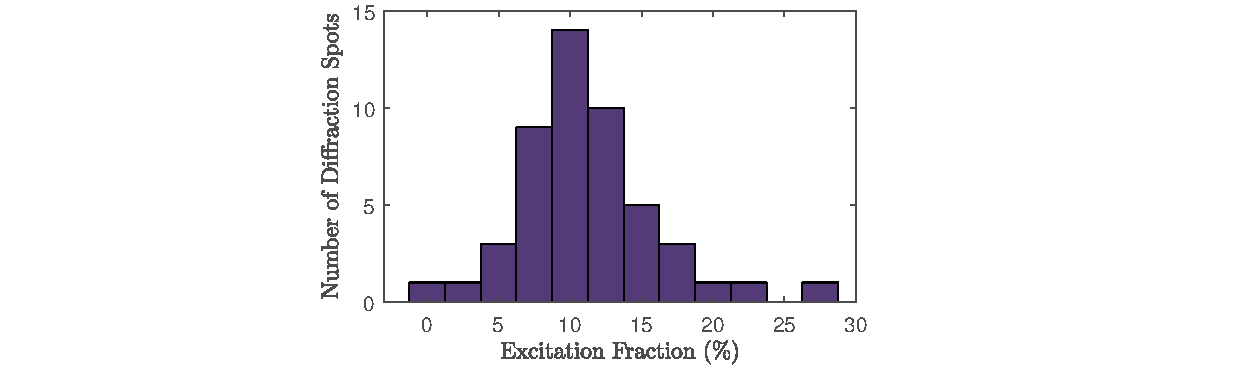
\includegraphics[width = \textwidth]{Figures/fig_UED_nexc.pdf}
  \caption{
  Histogram of the values of $\eta_\text{exc}$ determined by applying
  UED data to Eq.~\eqref{eq: nexc} when the photoproduct can be generated thermally.
  }
  \label{fig: UED-nexc}
\end{figure}

A third way to determine the excitation fraction can be used
if the molecular system exhibits significant changes in its lattice parameters
during the photoinduced and thermally-induced phase transitions.
In such a case, the spots of the diffraction pattern would shift in position
as the crystal lattice of the solid mixture distorts to accommodate
the two different sets of unit cells.
Assuming that the empirical rule known as Vegard's law%
\footnote{Norwegian physicist Lars Vegard (1880--1963) observed a linear relation between
the lattice parameters of ionic salt alloys and the concentration of each components
using XRD~\cite{Vegard1921, Denton1991}.}
%
holds in mixtures of photoexcited and ground state molecules,
a linear relation analogous to Eq.~\eqref{eq: coppens2}
can be stated as
%
\begin{equation}
  \begin{aligned}
    a_{j, \text{on}}(\infty)
      & = \eta_\text{exc} a_{j, \text{exc}}(\infty)
        + \left( 1 - \eta_\text{exc} \right) a_{j, \text{off}} \\
      & \approx \eta_\text{exc} a_{j, \text{HT}}
        + \left( 1 - \eta_\text{exc} \right) a_{j, \text{LT}}
  \end{aligned}
\end{equation}
%
and
%
\begin{equation}
  \begin{aligned}
    \eta_\text{exc}
      & = \frac{a_{j, \text{on}}(\infty) - a_{j, \text{LT}}}{a_{j, \text{HT}} - a_{j, \text{LT}}}
  \end{aligned}
  \label{eq: vegard}
\end{equation}
%
where $a_{j, \text{S}}$ is one of the three lattice parameters
in state $\text{S} = \{\text{on}, \text{off}, \text{HT}, \text{LT}\}$.

%%%%%%%%%%%%%%%%%%%%%%%%%%%%%%%%%%%%%%%%%%%%%%%%%%%%%%%%%%%%%%%%%%%%%%%%%%%%%%%%%%%%

\subsection{Data Analysis --- Part 3}
\label{sec: UED-data-analysis-3}

The data analysis of the original UED dataset has so far remained in the reciprocal space.
%
In Sec.~\ref{sec: UED-data-analysis-2}, data preprocessing has efficiently distilled
the multi-gigabyte stack of $\> 10^5$ UED images to
a single data matrix of relative intensity changes $\Delta I(\boldsymbol{t, q_i})$
integrated over the ROIs of the diffraction pattern.
%
In Sec.~\ref{sec: UED-data-analysis-3}, SVD-based global analysis reduced
the dimensionality of the data to a few key components that evolve over time;
calculation of the Pearson correlation coefficients projected
the evolving excited-state structure factors
$F_\text{exc}(\boldsymbol{t, q})$ as a trajectory
in the space of steady-state molecular configurations.
%
To finally make the titular `molecular movie' from the UED dataset,
a mapping from reciprocal to real space is necessary and
it is described in this section.

Recall from Eq.~\eqref{eq: Fsquared} that the crystal structure of a sample
could in principle be recovered by measuring its structure factors
$F(\boldsymbol{q}_j) = |F(\boldsymbol{q}_j)| \text{e}^{\text{i} \theta_j}$
and applying an inverse Fourier transform.
%
In practice, this is usually not possible
since the diffraction patterns of the sample is imaged by a CCD~camera
by simply counting the number of transmitted electrons and thus measuring only
the absolute value of the structure factors $|F(\boldsymbol{q}_j)|$.
%
Infamously known as the `phase problem' of crystallography,
the inaccessibility of the complex phases~$\theta_j$ means that
crystal structures are insufficiently constrained by their diffraction patterns
and cannot be uniquely determined so naively in general.
%
One solution is `molecular replacement':
replace the missing set of complex phases $\theta_j$ with values that
are derived from a structurally similar molecule (see Fig.~\ref{fig: phase-problem}
and Ref.~\cite{Taylor2003}).
%
In the works of this thesis, it is also the solution of choice since
the ground state structure of all the target molecules is already known
to a high degree of precision.
%
If there is a state $\text{S}_1$ proximate to the photoexcited state
that is either thermally accessible or metastable and long-lived,
an end structure would also be available in the literature;
a candidate structure with atomic positions $\bscriptr_{i, \text{exc}}$ for the transient state
that exists at each time point $t$ can then be modeled as a linear combination
of the two known structures,
%
\begin{equation}
  \begin{aligned}
    \bscriptr_{i, \text{exc}} & = \bscriptr_{i, \text{S}_0}
      + \xi_i \left( \bscriptr_{i, \text{S}_1} - \bscriptr_{i, \text{S}_0} \right)
  \end{aligned}
  \label{eq: linear-model}
\end{equation}
%
where $\xi_i$ is the scaling factor for the displacement of atom $i$ of $N_\text{at}$.

% Phase problem
\begin{figure}[t!]
  \centering
  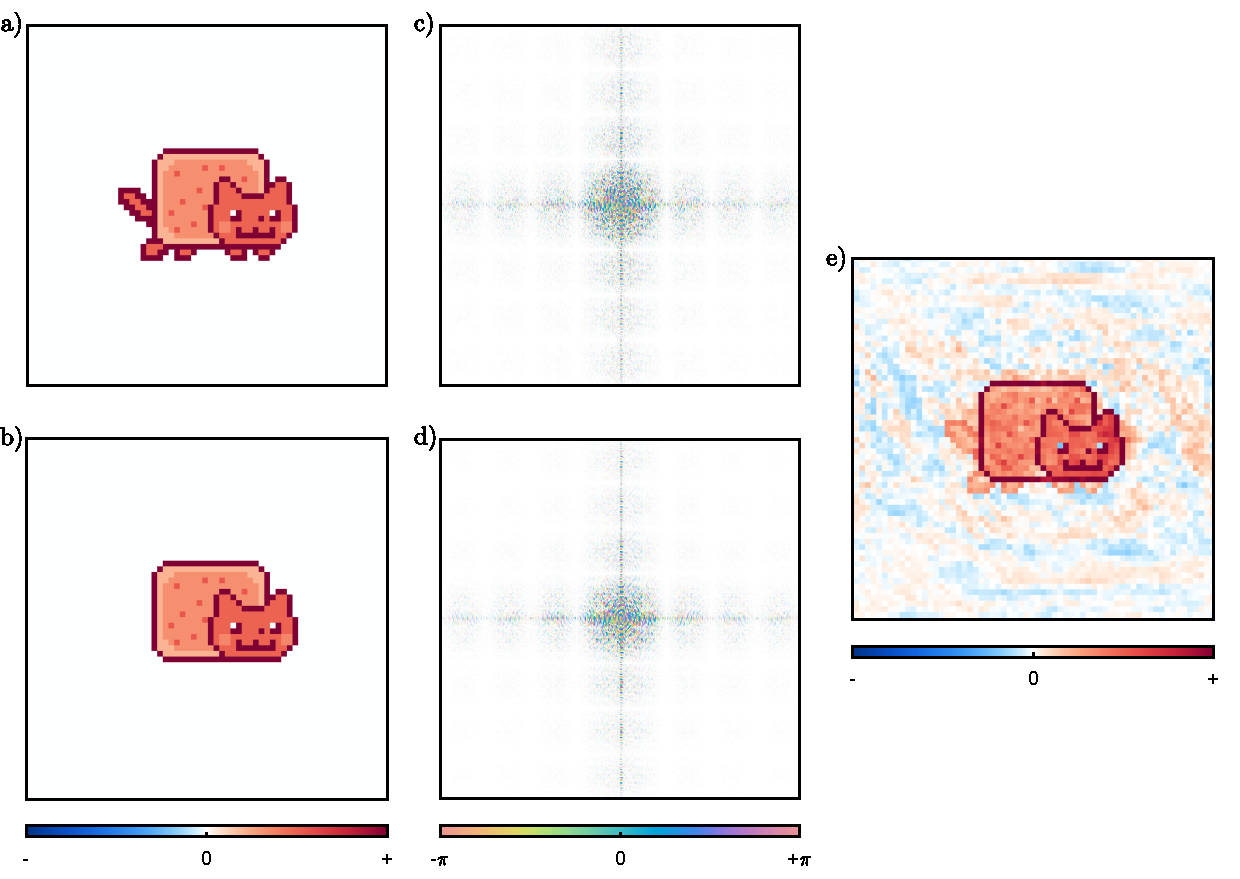
\includegraphics[width = \textwidth]{Figures/fig_ch2_nyancat.pdf}
  \caption[Phasing by molecular replacement.]{
    Phasing by molecular replacement.
    Electron diffraction maps the real-space electrostatic potential of the target
    into reciprocal space, here represented by (a)~a positive semi-definite image of a cat and
    (c)~its complex-valued Fourier transform.
    %
    Generally, information is partly lost when only the amplitude of the scattered wavefunction
    in the form of diffraction intensities is measured.
    %
    Given (b) a similar real-space distribution and (d) its known complex phase,
    the information loss can be reversed by phase substitution,
    resulting in (e) an hybrid that approximates the original.
  }
  \label{fig: phase-problem}
\end{figure}

To efficiently apply Eq.~\eqref{eq: Fsquared} and calculate the structure factors
of a given molecular model for a range of $\boldsymbol{q}$ values,
a popular analytical approximation of the electron elastic atomic scattering factors~$f(\boldsymbol{q})$
is used. From~\cite{Ren1996}, it is in the form of
%
\begin{equation}
  \begin{aligned}
    f_Z(\boldsymbol{q}) & = \sum_{n = 1}^6 a_n \text{e}^{- b_n (q/4 \unslant[-.2]\pi)^2}
  \end{aligned}
  \label{eq: fparameters}
\end{equation}
%
where $a_n, b_n$ are parameters fitted to the scattering data of each element with atomic number $Z$;
those used in the calculations of this thesis are plotted in Fig.~\ref{fig: UED-fparameters}
and tabulated in App.~\ref{ap: fparameters} for reference.

\begin{figure}[t!]
  \centering
  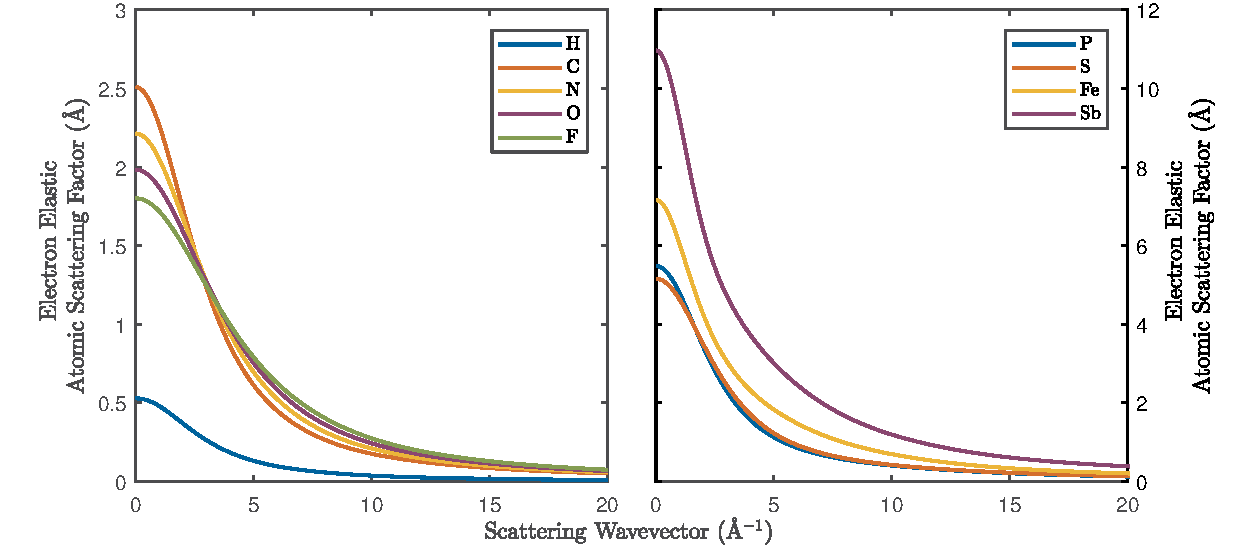
\includegraphics[width = \textwidth]{Figures/fig_UED_fparameters.pdf}
  \caption{
  Plot of the electron elastic atomic scattering factors $f(\boldsymbol{q})$ for select atoms,
  parameterized according to Eq.~\eqref{eq: fparameters}~\cite{Ren1996}.
  }
  \label{fig: UED-fparameters}
\end{figure}

% Diffraction pattern simulation
From Sec.~\ref{sec: UED-cryst}, the intensity distribution of
an electron diffraction pattern is shaped by more than just
the value of the structure factors of the sample.
%
As seen in Fig.~\ref{fig: ewald}b, experimental imperfections
affect the geometry of the scattering process and
consequently relax the Laue-Bragg condition for diffraction.
%
Thus, to generate an accurate set of diffraction intensities
for comparison with experimental results, a simulation scheme is setup in the way of
the Ewald construct, wherein the structure factor values are calculated at
the points $\boldsymbol{q}$ which are at the intersection of the Ewald sphere and
the reciprocal lattice $\boldsymbol{g}_{h_1 h_2 h_3} = \sum \limits_{i = 1}^3 h_i \boldsymbol{b}_i$.

The Ewald sphere constrains the calculation to the set of scattered wavevectors
permissible under elastic scattering,
%
\begin{equation}
  \begin{aligned}
    | \boldsymbol{q} - \boldsymbol{k}_\text{inc} | = k_\text{inc}
  \end{aligned}
\end{equation}
%
where $\boldsymbol{k}_\text{inc}$ is the wavevector of the incident probe electrons,
with amplitude $k_\text{inc} = \frac{2 \unslant[-.2]\pi}{\lambda}$ and
direction $\hat{\boldsymbol{k}}_\text{inc} \parallel \sum \limits_{i = 1}^3 u_i \boldsymbol{a}_i$.
%
Under this definition, the crystal orientation is held fixed while the incident direction
is referred by either $[ u_1, u_2, u_3 ]$ in the Miller notation%
\footnote{The letters $u, v, w$ are used most often to refer to crystal orientations;
however, numbered subscripts are used instead here for convenient indexing.}
or simply $\theta_\text{inc}, \phi_\text{inc}$ in spherical coordinates.

The points of the reciprocal lattice are modeled as Gaussian-shaped relrods.
Any $n$ relrods within the range of a diffraction spot cumulatively contribute
to the value of the structure factor at $\boldsymbol{q}$,
%
\begin{equation}
  \begin{aligned}
    f(\boldsymbol{q}) & = \text{e}^{-2W} \sum_{n} f(\boldsymbol{g}_n) \text{e}^{- \frac{1}{2} s_n^2 / \sigma^2}
  \end{aligned}
  \label{eq: relrods}
\end{equation}
%
where $\boldsymbol{g}_n$ is the position of the relrods near $\boldsymbol{q}$,
$s_n = |\boldsymbol{q} - \boldsymbol{g}_n|$ is the `excitation error' or
the deviation from the Laue-Bragg condition,
$W = \frac{1}{6} q^2 \left< \delta \scriptr^2 \right> $ is the Debye-Waller factor,
and $\sigma^2 = \sigma_\text{sh}^2 + (\sigma_\text{ph} q)^2$ is the width of the relrods;
$\sigma_\text{sh}$ is the contribution due to the shape factor $S(\boldsymbol{q})$ in
Eq.~\eqref{eq: diff-int} and $\sigma_\text{ph}$ is
a phenomenological parameter included to account for imperfections such as
crystal mosaicity and divergence of the probe beam.

To transform the $(q_x, q_y, q_z)$ coordinates in reciprocal space to the $(x, y, z)$ coordinates
of the UED images, a three-dimensional rotation is first made to align $\boldsymbol{k}_\text{inc}$
with $\hat{\boldsymbol{q}_z}$ using Rodrigues' rotation formula,%
\footnote{French mathematician Benjamin Olinde Rodrigues (1795--1851) discovered in 1840
this convenient formula to rotate a vector in three dimensional space
given an axis and an angle of rotation~\cite{Murray1994}.}
%
\begin{equation}
  \begin{aligned}
    \boldsymbol{q}
      & \rightarrow \boldsymbol{q} \cos \theta
        + (\hat{\boldsymbol{k}} \times \boldsymbol{q}) \sin \theta_\perp
        + \hat{\boldsymbol{k}} (\hat{\boldsymbol{k}} \cdot \boldsymbol{q}) (1 - \cos \theta)
  \end{aligned}
  \label{eq: rodrigues1}
\end{equation}
%
where $\hat{\boldsymbol{k}} = \frac{\hat{\boldsymbol{k}}_\text{inc} \times \hat{\boldsymbol{q}}_z}{ \sin \theta}$
and $\theta = \operatorname{arcos}(\hat{\boldsymbol{k}}_\text{inc} \cdot \hat{\boldsymbol{q}_z})$.
%
Alternatively,
%
%
\begin{equation}
  \begin{aligned}
    \boldsymbol{q} & \rightarrow \mathbf{R}(\theta) \boldsymbol{q}
  \end{aligned}
  \label{eq: rodrigues2}
\end{equation}
%
where
%
\begin{equation}
  \begin{aligned}
    \mathbf{R}(\theta) & = \mathbf{I} + \mathbf{K} \sin \theta  + \mathbf{K}^2 (1 - \cos \theta) \\
    \mathbf{K} & =
      \begin{bmatrix}
          0 & -k_z & k_y \\
          k_z & 0 & -k_x \\
          -k_y & k_x & 0
      \end{bmatrix}
  \end{aligned}
  \label{eq: rodrigues3}
\end{equation}
%
Finally, $\boldsymbol{q}$ is projected onto the camera frame and converted into units of image pixels
using the camera parameter (see Fn.~\ref{fn: camera-parameter}).

Altogether, the simulation of an electron diffraction pattern requires as input the following:
$N_\text{at} \times 3$ fractional atomic coordinates, the six lattice constants
($a_1, a_2, a_3$ and $\alpha_{23}, \alpha_{31}, \alpha_{12}$),
the camera parameter (${\sim}1.39 \times 10^{-2}$~\AA$^{-1}$/px),
the incident electron energy (95~keV) and direction $[u_1 u_2 u_3]$,
the Debye-Waller thermal variance $\left< \delta \scriptr^2 \right>$, and
the relrod widths $\sigma_\text{sh}, \sigma_\text{ph}$.
%
The value of the last six parameters are unique to each experiment and
they need to be determined with some precision.
%
This is achieved by first simulating the structure factors $F_\text{sim}(\boldsymbol{q})$
of the ground state using its known crystallographic information from XRD
for all possible orientations $\theta_\text{inc}, \phi_\text{inc}$
and maximizing the value of the Pearson correlation coefficient between the simulated
and experimental datasets $P_\text{sim, exp}$ (see Fig.~\ref{fig: UED-orientation}).
From this rough orientation, the other three parameters are refined using least-square fitting.

\begin{figure}[t!]
  \centering
  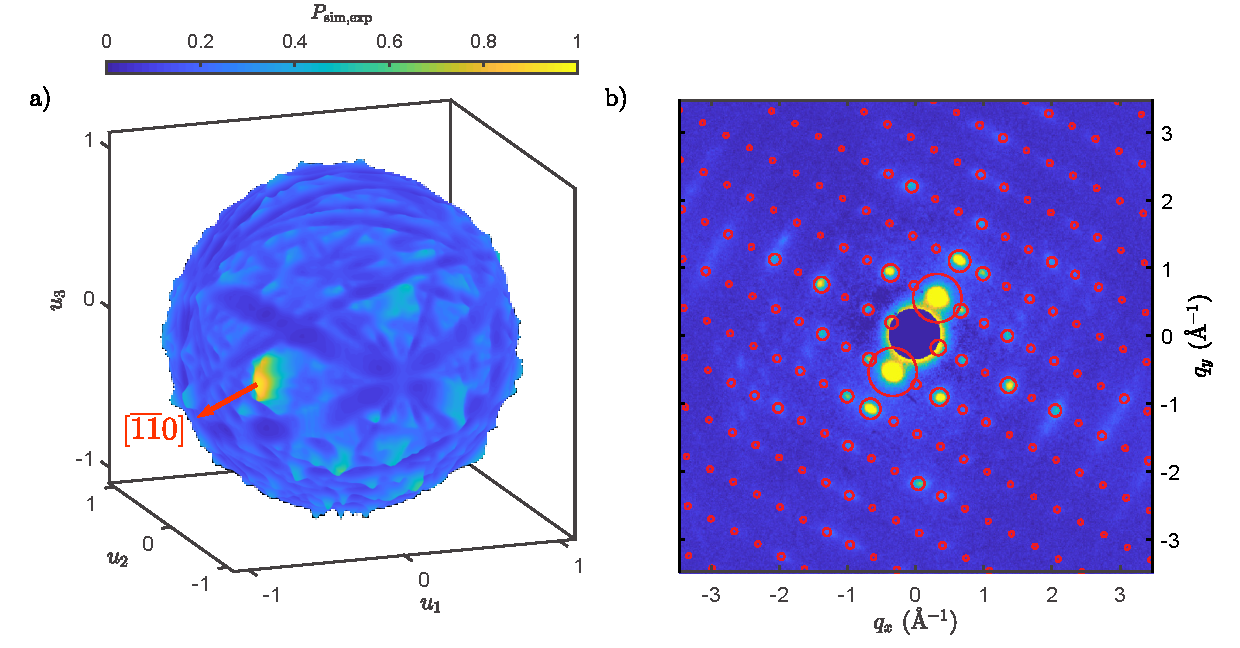
\includegraphics[width = \textwidth]{Figures/fig_UED_orientation.pdf}
  \caption[Determination of the incident direction of the probe electrons relative to the sample.]{
  Determination of the incident direction of the probe electrons relative to the sample:
  (a) for each possible direction, a diffraction pattern is simulated and compared with
  the experimental one by calculating their Pearson correlation coefficient $P_\text{sim, exp}$;
  (b) in the direction of peak correlation, there is optimal match between the simulated
  and experimental diffraction intensity. The size of the circles in Panel (b) is proportional to
  the value of $F_\text{sim}(\boldsymbol{q})$.
  }
  \label{fig: UED-orientation}
\end{figure}

% Molecular movie
Now that a scheme for accurately simulating UED data has been defined and optimized,
it can be applied to the structures generated by Eq.~\eqref{eq: linear-model}.
The resulting values of $F_\text{exc, sim}(\boldsymbol{\xi}, \boldsymbol{q}_j)$
are combined with the excitation fraction $\eta_\text{exc}$ in Eq.~\eqref{eq: coppens}
to produce simulated values that are representative of the `pump on' state,
%
\begin{equation}
  \begin{aligned}
    F_\text{on, sim}(\boldsymbol{\xi}, \boldsymbol{q}_j)
      & = \eta_\text{exc} F_\text{exc, sim}(\boldsymbol{\xi}, \boldsymbol{q}_j)
        + \left( 1 - \eta_\text{exc} \right) F_\text{off, sim}(\boldsymbol{q}_j)
  \end{aligned}
\end{equation}
%
which can then be compared with the time-dependent experimental structure factors values
$F_\text{on, exp}(t, \boldsymbol{q})$
--- extracted using the methods described in Sec.~\ref{sec: UED-data-analysis-2} ---
by calculating their Pearson correlation coefficient
%
\begin{equation}
  \begin{aligned}
    P_\text{sim, exp}(\boldsymbol{\xi}, t)
      & = \frac{\text{cov}(\zeta_\text{on, sim}(\boldsymbol{\xi}, \boldsymbol{q}_j), \zeta_\text{on, exp}(t, \boldsymbol{q}_j))}{\sigma_\text{on, sim} \sigma_\text{on, exp}}
  \end{aligned}
\end{equation}
%
and using it as a measure of the `goodness of fit' between the model structure
parameterized by $\boldsymbol{\xi}$ and the sought-after time-dependent structure of the photoexcited state.
%
Hence, to make the putative molecular movie, it is only a matter of maximizing
$P_\text{sim, exp}(\boldsymbol{\xi}, t)$ to find a $\boldsymbol{\xi}_\text{opt}(t)$
that reproduces the structural dynamics of the UED observations.
%
However, it is computationally too onerous to perform optimization on a function that
has so many independent variables, given that there are as many $\xi_i$ as atoms in the unit cell
of the sample.

A solution is to apply the principle of dimensionality reduction to aforementioned structure model.
From Sec.~\ref{sec: UED-data-analysis-2}, it can be argued that the plethora of redundant complexity in
reciprocal space suggests that molecular systems do not fully explore their configuration space
in all its $(3 N_\text{at} - 6)$-dimensional glory but instead live within a subspace spanned
by a few key reaction coordinates.
%
In this view, it is herein assumed that the $N_\text{at}$ atoms in the unit cell
can be partitioned into $N_G \ll N_\text{at}$ `dynamical groups'
within which member atoms move in lockstep, i.e. $\xi_i = \xi_j \enskip \forall \enskip i,j$ in
the group.
%
To determine which groupings amongst the infinitely many possible ones to test for optimization,
a first-principles approach based in `chemical intuition' can be employed as a preliminary to
future theoretical work involving quantum chemical calculations and molecular dynamics simulations.
%
It is recognized that molecules are generally composed of atoms or groups of atoms
which behave similarly whenever they occur in different compounds.
These assemblies are referred to as `functional groups' or `moieties' of the molecule
and those which preserve the symmetry of the unit cell constitute a reasonable guess of the dynamical groups
necessary to describe the observed structural dynamics.
%
This method is demonstrated in Fig.~\ref{fig: UED-molecularmovie} using the data
from the UED experiment on (EDO-TTF)\textsubscript{2}PF\textsubscript{6} (see Ch.~\ref{ch: UED-EDO}).

\begin{figure}[t!]
  \centering
  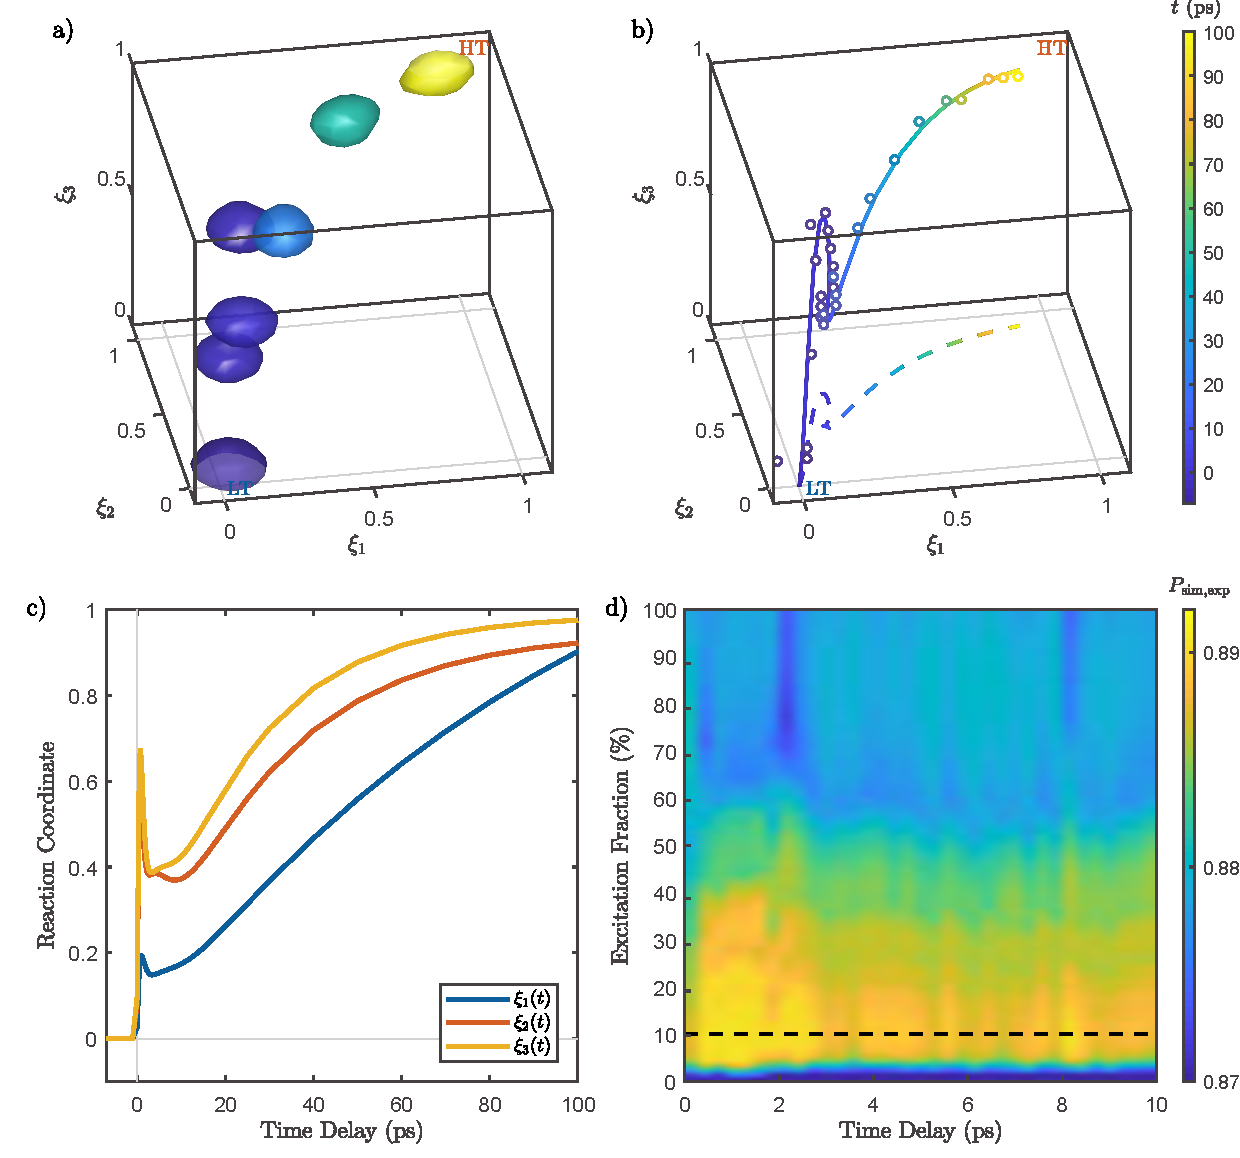
\includegraphics[width = \textwidth]{Figures/fig_UED_molecularmovie_.pdf}
  \caption[Making a molecular movie from UED data.]{
    Making a molecular movie from UED data:
    (a) isosurface plot of $P_\text{sim, exp}(\boldsymbol{\xi}, t)$ at different time delays
    in $\boldsymbol{\xi}$-space, with a cut-off at 95\% of the global maximum;
    (b) plot of $\boldsymbol{\xi}_\text{opt}(t)$ along with its fit line
    from a multi-exponential global fitting model;
    (c) plot of the fit lines of $\boldsymbol{\xi}_\text{opt}(t)$ as independent functions;
    (d) surface plot of $P_\text{sim, exp}(\boldsymbol{\xi}_\text{opt}, t)$ for a range of $\eta_\text{exc}$
    values, illustrating the temporal constancy of $\eta_\text{exc}$ and providing another way to confirm
    its value as calculated in Sec.~\ref{sec: UED-data-analysis-2}.
  }
  \label{fig: UED-molecularmovie}
\end{figure}

Three dynamical groups, parameterized by the reaction coordinates $\xi_1, \xi_2, \xi_3$, are constructed
by imposing inversion symmetry on the six moieties in the unit cell,
with the ground and end states specified by $\boldsymbol{\xi}  = (0, 0, 0)$ and $(1, 1, 1)$ respectively.
%
In Panels~(a)--(c), a well-behaved and strongly peaked $P_\text{sim, exp}(\boldsymbol{\xi}, t)$
can be seen in the space of $\boldsymbol{\xi} = (\xi_1, \xi_2, \xi_3)$,
suggesting that structural refinement at every time delay is readily achievable using this particular grouping;
in Panel~(d), optimization over $\eta_\text{exc}$ yields a sensible value that is consistent with
the calculations in Sec.~\ref{sec: UED-data-analysis-2} and
constant over the duration of the structural dynamics.

  
\chapter{Ultrafast Structural Dynamics of (EDO-TTF)\textsubscript{2}X}
\label{ch: UED-EDO}

In this chapter, I will present two studies on the photoinduced structural dynamics
of the crystalline material (EDO-TTF)\textsubscript{2}X. For context,
a general overview of this molecular system will be given. This is followed by a description
of the experimental procedure and a discussion of the results from the studies.
The works herein have been reported in the articles
``Mapping Molecular Motions Leading to Charge Delocalization with Ultrabright Electrons''
and ``Ultrafast Electron Diffraction Study of Single-Crystal
(EDO-TTF)\textsubscript{2}SbF\textsubscript{6}: Counterion Effect and Dimensionality Reduction,''
previously published in the journals Nature and Chemical Physics Letters respectively~\cite{Gao2013, Liu2017}.

\section{Overview of (EDO-TTF)\textsubscript{2}X Molecular Systems}
\label{sec: UED-EDO-overview}

In 1941, Albert Szent-Gy\"{o}rgyi%
\footnote{Albert Szent-Gy\"{o}rgyi (1893--1986) is a Hungarian biochemist
who won the Nobel Prize in Physiology or Medicine in 1937
for his work in vitamin C and the chemistry of cellular respiration~\cite{Nobel1922}.}%
proposed that some processes in biological systems, such as photosynthesis,
could be explained by long-range light-induced transfer of electrons
through a chain of interacting proteins in a manner analogous to electrical conduction in metals
as described by band theory~\cite{Szent1941, Szent1946}.
%
Such an `organic metal' would combine the mechanical and functional versatility of an organic%
\footnote{`Organic' originally refers to that which is solely derived from living organisms;
it has now been generalized to describe chemistry that involves the element carbon,
often in association with other nonmetals.}
compound with the electron transport properties of a conventional metal ($\sigma \gtrsim 10^3$~S/cm,
see Fig.~\ref{fig: EDO-overview}a).
%
\begin{figure}[ht!]
  \centering
  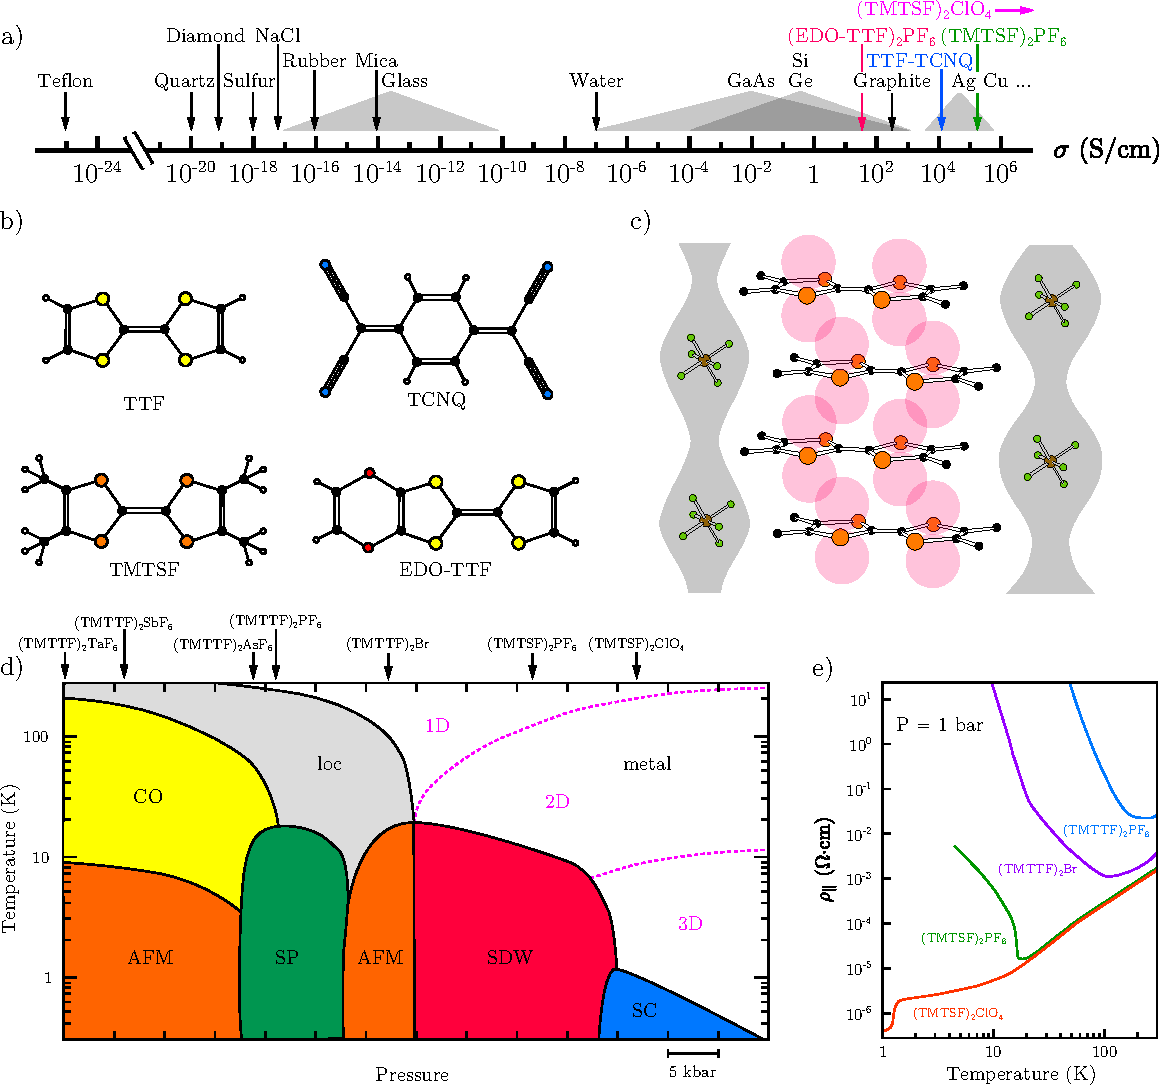
\includegraphics[width = \textwidth]{Figures/fig_EDO_overview.pdf}
  \caption[Overview of organic metallicity.]{
  Overview of organic metallicity.
  (a) Electrical conductivity of various materials for comparison~\cite{CRCHandbook, TTFBook}.
  (b) Structural building blocks of Bechgaard-Fabre salts and related compounds
  (white = hydrogen, black = carbon, blue = nitrogen, red = oxygen, green = fluorine, brown = phosphorus, orange = selenium).
  (c) Schematic of the crystal structure of (TMTSF)\textsubscript{2}PF\textsubscript{6},
  showing the overlapping regions of positive (pink) and negative (gray) charge
  that enable electrical conduction.
  (d) Generalized phase diagram of Bechgaard-Fabre salts;
  behaviour at standard ambient pressure is indicated by arrows at top;
  abbreviations: `loc' = localization, `CO' = charge ordering, `SP' = spin-Peierls,
  `AFM' = antiferromagnetism, `SDW' = spin-density wave, `SC' = superconductivity, `ND' = n-dimensional;
  solid lines represent phase transitions while dashed lines are crossovers.
  (e) Electrical resistivity $\rho_\parallel$ along the stacking axis
  as a function of temperature at standard ambient pressure;
  note the superconductive transition of (TMTSF)\textsubscript{2}ClO\textsubscript{4}.
  Panels~(c)--(e) are adapted with permission from
  Refs.~\cite{BechgaardJerome1982, Dressel2007, Jerome1982} respectively.
  }
  \label{fig: EDO-overview}
\end{figure}
%
This prospect stimulated significant interest amongst chemists and material scientists,
leading to the discovery of moderately conductive but short-lived compounds like perylene--bromine
($\sigma \sim 1$~S/cm) in 1954~\cite{Akamatu1954} and a proposal by William A. Lamb in 1964
of a synthetic organic polymer that remains superconductive at room temperature~\cite{Little1964}.

A major breakthrough came in 1977 when Shirakawa and his collaborators%
\footnote{This work netted the 2000 Nobel Prize in Chemistry
for Alan J. Heeger (1936--present), Alan G. MacDiarmid (1927--2007),
and Hideki Shirakawa (1936--present)~\cite{Nobel1996}.}
%
discovered that doping \textit{trans}-polyacetylene with iodine vapour
can increase its electrical conductivity by seven orders of magnitude,
reaching $\sigma = 38$~S/cm at room temperature~\cite{Shirakawa1977}.
Around the same time, Coleman, Ferraris, and their coworkers combined
two recently discovered molecules, tetrathiafulvalene~(TTF) and
tetracyano-\textit{p}-quinodimethane~(TCNQ),
to prepare a 1:1 complex that, when crystallized,
conducts like a metal over a large range of temperature
($\sigma_\text{max} = 1.47 \times 10^4$~S/cm)~\cite{Wudl1970, Coleman1973, Ferraris1973}.

The molecule TTF-TCNQ was not simply the result of serendipity but a sagacious feat of molecular design.
%
High electron mobility requires good overlap of valence orbitals
that are not completely filled, thus allowing electrons to easily move from one molecule to another.
However, this requirement also tends to destabilize the material
as the unpaired valence electrons make it susceptible to chemical attack by other substances.
%
It happens that TTF and TCNQ can readily donate and accept electrons
while remaining chemically stable because of the aromaticity%
\footnote{A molecule is said to be aromatic when it has a flat ring of atoms
bound together by an set of overlapping p orbitals.}
of the resulting radical ions, TTF$^+$ and TCNQ$^-$~\cite{LittleBook}.

When crystallized together, TTF and TCNQ molecules self-assemble into
separate stacks of molecules lying parallel to each other
as each species interacts amongst themselves through their heteroatoms and
$\unslant[-.2]\pi$~orbitals (see Fig.~\ref{fig: EDO-overview}b).
%
A partial charge transfer (ca.~$0.56$~e$^-$) occurs and the ions flatten,
further overlapping the $\unslant[-.2]\pi$ orbitals within each stack and
forming an array of conductive wires through the crystal
in the direction of the stacking axis.

In the absence of significant interstack orbital overlap,
bulk TTF-TCNQ behaves as a loose ensemble of
quasi-one-dimensional electron systems, which are highly susceptible to
Peierls instability,%
\footnote{Rudolf E. Peierls (1907--1995) noted in 1954 that
one-dimensional periodic arrangements of atoms with delocalized electrons
tend to dimerize due to electron--phonon coupling~\cite{PeierlsBook}.
}
%
a cooperative phenomenon that eventually destroys the conductive state of TTF-TCNQ
at low temperature ($T \approx $~38--54~K).
%
In a bid to stave off this metal--insulator~(MI) phase transition,
Bechgaard, Fabre, and their coworkers synthesized a new class of
charge-transfer~(CT) compounds based on molecular design principles
similar to those of TTF-TCNQ~\cite{Bechgaard1980}.
%
Known as Bechgaard-Fabre salts,%
\footnote{Named for Danish chemist Klaus Bechgaard (1945--2017) and
French chemist Jean-Marc Fabre (1943--present) who respectively
first synthesized the selenium (TMTSF) and sulfur (TMTTF) derivatives of TMTCF~\cite{Pouget2012}.}
%
they have the chemical formula (TMTCF)\textsubscript{2}X,
where TMTCF$^{0.5+}$ is tetramethyl-tetrachalcofulvalene
and X is a monovalent weakly-coordinating anion like
hexafluoropnictate (PnF\textsubscript{6}$^-$).%
\footnote{Chalcogens are chemical elements in group 16 of the periodic table, e.g.~sulfur and selenium;
pnictogens are those in group 15, e.g.~phosphorus and antimony.}

When crystallized, (TMTCF)\textsubscript{2}X forms a strongly anisotropic material
as the flat cations assemble in parallel, into conductive stacks separated by columns of isolated anions
(see Fig.~\ref{fig: EDO-overview}c for a schematic view).
%
Given this lattice structure and the resulting electronic system,
competing interactions and a subtle interplay
of the charge, spin, and nuclear degrees of freedom
give rise to a variety of collective phenomena~\cite{Kohler2011}.
%
In Fig.~\ref{fig: EDO-overview}d,
a generalized phase diagram of Bechgaard-Fabre salts is shown;
it is replete with ground states separated by phase transitions and crossovers
that can be induced by fine-tuning the coupling within and between the molecular stacks
through pressure --- externally applied
or chemically induced via anion substitution~\cite{Jerome1991}.
%
In 1980, it was discovered that superconductivity could be achieved in
(TMTSF)\textsubscript{2}PF\textsubscript{6} at $T \leq 1.3$~K
by applying $>6$~kBar of pressure~\cite{Bechgaard1980, Jerome1980};
one year later, the perchlorate (ClO\textsubscript{4}$^-$) salt was found
to become superconductive at about the same temperature but under standard ambient pressure
(Fig.~\ref{fig: EDO-overview}e)~\cite{Bechgaard1981, Jerome1982}.

From above, it is clear that the material properties of Bechgaard-Fabre salts depend crucially on
the network of orbital overlaps and weak intermolecular interactions throughout the crystal lattice.
%
To explore this rich physics, numerous other derivatives of prototypical TTF~molecule have been synthesized
by attaching functional substituents to both or either side of the TTF~core.
%
One of them is 4,5-ethylenedioxy-tetrathiafulvalene (EDO-TTF)~\cite{Papavassiliou1990, Mori1990, Meziere2000}
and its 2:1 radical-cation salts (EDO-TTF)\textsubscript{2}X
have been observed to exhibit a MI phase transition upon cooling
unlike any other before~\cite{Ota2002, Ota2003, Ota2006}.

\begin{figure}[ht!]
  \centering
  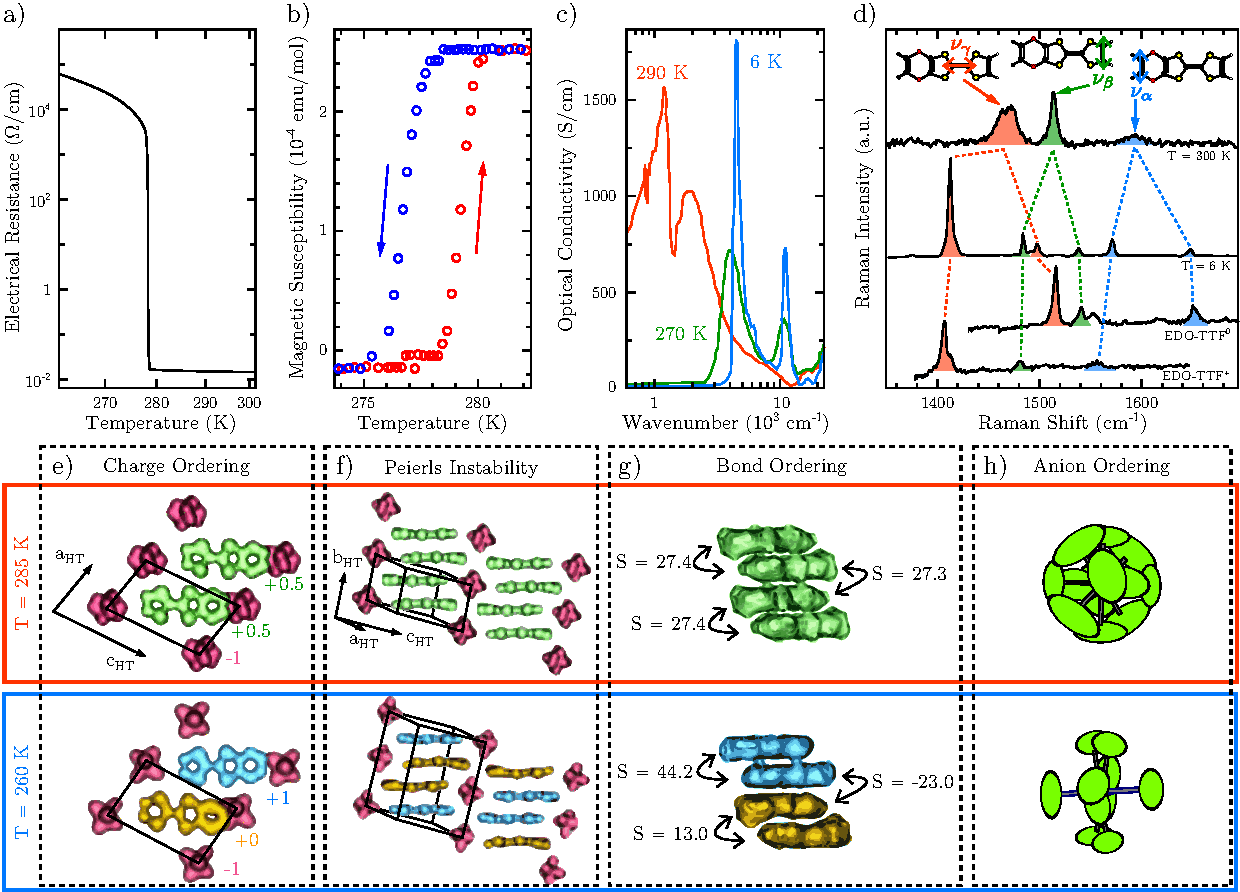
\includegraphics[width = \textwidth]{Figures/fig_EDO_static.pdf}
  \caption[Metal--insulator phase transition in (EDO-TTF)\textsubscript{2}PF\textsubscript{6}.]{
  Metal--insulator phase transition in (EDO-TTF)\textsubscript{2}PF\textsubscript{6}.
  Temperature dependence of (a) electrical resistivity, (b) magnetic susceptibility,
  and (c) optical conductivity along the stacking axis.
  (d) Raman spectra of (EDO-TTF)\textsubscript{2}AsF\textsubscript{6}
  above and below $T_\text{MI}$, along with that of neutral EDO-TTF and
  (EDO-TTF)$^+$(IBr\textsubscript{2})$^-$;
  peaks associated with charge-sensitive C=C stretching modes are color-coded.
  Charge density isosurfaces (0.7~e$^-$/\AA$^3$) calculated from XRD data,
  as viewed (e) along the stacking axis and (f) from the side,
  coloured by charge state (blue: $+1e$, green: $+0.5e$, yellow: $+0e$, red: $-1e$);
  (g) lower isosurfaces (ca.~$0.1$~e$^-$/\AA$^3$)
  with relevant orbital overlap integral values $S$ ($\times 10^{-3}$).
  (h) Thermal ellipsoids of the PF\textsubscript{6} anions.
  Panels~(a), (b), and (g) are adapted with permission from Ref.~\cite{Ota2002};
  (c) and (d), from Refs.~\cite{Drozdova2003, Drozdova2004} respectively;
  (e)--(f), from Ref.~\cite{Aoyagi2004}.
  }
  \label{fig: EDO-static}
\end{figure}
%
At room temperature, single-crystal (EDO-TTF)\textsubscript{2}PF\textsubscript{6}
appears black and is highly reflective.
%
As seen in Fig.~\ref{fig: EDO-static}a,
the electrical conductivity decreases abruptly at $279.0$~K from $60$~S/cm to
$1.4 \times 10^{-5}$~S/cm and subsequently varies with an activation energy of $0.52$~eV,
indicating a first-order MI phase transition from a high-temperature (HT) metallic phase
to a low-temperature (LT) insulator phase at $T_\text{MI} = 279.0$~K.
%
This is observed again with optical conductivity measurements (Fig.~\ref{fig: EDO-static}c),
which show the simultaneous disappearance of a broad Drude%
\footnote{German physicist Paul Drude (1863--1906) studied optical phenomena
from the perspective of electromagnetism and introduced a classical model of metals
to explain their transport properties~\cite{DrudeBioBook}.}
feature typical of metals and the appearance of two sharp peaks at 4500~cm$^{-1}$ and 11150~cm$^{-1}$.

XRD measurements of the HT phase reveal a triclinic crystal structure with P$\overline{1}$ symmetry,
not too dissimilar to those of (TMTCF)\textsubscript{2}X:
`nearly flat' EDO-TTF molecules stacked perpendicularly in a head--tail arrangement
with PF\textsubscript{6} molecules at cell vertices,
slotted in the soft cavities formed by the terminal ethylene groups.
Overlapping $\unslant[-.2]\pi$~orbitals along the stacking axis form
a quasi-1D electronic band structure that becomes $\frac{3}{4}$-filled%
\footnote{Hole-wise, $\frac{1}{4}$-filled; each of the two EDO-TTF molecules has two valence electrons
and one of the four in total is transferred to the PF\textsubscript{6} molecule.}
during the CT process.
%
The LT phase has a significantly different crystal structure:
the P$\overline{1}$ triclinic unit cell is doubled along the stacking axis
to include four EDO-TTF molecules,
alternating pairwise between two nonequivalent --- `flat' and `bent'%
\footnote{The curvature of the EDO-TTF molecule refers to the sum of
the dihedral angles of the atom chain O--C--S--C and C=C--S--C;
`flat': 1.87$^\circ$, `nearly flat': 2.08$^\circ$, `bent': 13.42$^\circ$.} ---
structures and two PF\textsubscript{6} molecules that are displaced from
the highly symmetric cell vertices.
%
These concomitant pairwise symmetry-breaking structural distortions indicates that
the MI phase transition is in part driven by Peierls instability.
This cooperativity is also evidenced by the bistability of phases seen in
the thermal hysteresis of the magnetic susceptibility (Fig.~\ref{fig: EDO-static}b).

Close inspection of the charge density reconstructed from the XRD data reveals
other unexpected differences between the LT and HT phases.
As seen in Fig.~\ref{fig: EDO-static}g, a `bond order' is apparent
when the intermolecular distances and orbital overlap integral values are calculated~\cite{Aoyagi2004};
below $T_\text{MI}$, bonding along the EDO-TTF stack strengthens
between the pairs of flat molecules while it weakens between the bent ones and
disappears between the dimers.

Furthermore, there is `anion ordering'~\cite{Ota2002}.
From Fig.~\ref{fig: EDO-static}h,
the PF\textsubscript{6} anions in the metallic HT phase are located at the inversion centres
of the unit cell and exhibit rotational disorder whilst the fluorine atoms are isotropically distributed
with large thermal ellipsoids.
%
In the insulator LT phase, the anions are displaced
from their special position of symmetry in the direction of the EDO-TTF stacking axis
and become uniaxially oriented as the atomic displacement parameters of the fluorine atoms
are drastically reduced and the F--P--F bonds point to the sulfur atoms on the neighbouring EDO-TTF molecules.
%
This suggests that the counterions are not merely spectating the MI phase transition
but are actively affected by the bond-coupled Peierls-type phonons of the EDO-TTF cations
through electrostatic interactions~\cite{Aoyagi2004}.

In Fig.~\ref{fig: EDO-static}d,
Raman spectra of (EDO-TTF)\textsubscript{2}X taken at different temperatures show splitting and shifting
of peaks associated with C=C stretching modes that are sensitive to the molecular charge.
Comparison with the spectrum of neutral and charged molecules suggests that the LT phase is composed of
electron donors in two different charge states~\cite{Drozdova2004}.
%
Analysis of charge-sensitive bond lengths~\cite{Ota2002} and
electron counting using XRD-derived charge densities~\cite{Aoyagi2004} further assign
a charge state of +0.5 to the nearly flat EDO-TTF molecules of the HT phase and
$+1e$ and $+0e$ to the flat and bent molecules of the LT phase respectively.%
\footnote{More precisely, nearly flat: $+(0.6 \pm 0.1)e$,
flat: $+(0.8 \pm 0.1)e$, and bent: $+(0.2 \pm 0.1)e$~\cite{Aoyagi2004}.}
%
Hence, a `charge order' commensurate with the previously described bond order
emerges during the MI~phase transition
as the charge-distributed state --- denoted D$^{+0.5}$D$^{+0.5}$D$^{+0.5}$D$^{+0.5}$ or $(\frac{1}{2} \frac{1}{2} \frac{1}{2} \frac{1}{2})$ ---
that is present in the metallic HT phase undergoes disproportionation and molecular deformation at $T_\text{MI}$,
transforming into the charge-localized $(1001)$ state of the insulator LT phase
(Fig.~\ref{fig: EDO-static}e--f).

It is remarkable that the $(1001)$ state of the LT phase is stable
since intuition would have instead given way to an alternating Wigner-type%
\footnote{Hungarian physicist and Nobel laureate Eugene P. Wigner (1902--1995) predicted in 1934
that a free electron gas would crystallize in the limit of zero kinetic energy~\cite{Nobel1963, Wigner1934}.}
$(1010)$ charge state wherein on- and off-site Coulomb repulsion would have been minimized,
as in the case of other quasi-1D molecular systems like
(DI-DCNQI)\textsubscript{2}Ag and (TMTTF)\textsubscript{2}PF\textsubscript{6}~\cite{Seo1997, Hiraki1998, Chow2000}.
%
However, this simplistic assessment ignores the energetic contribution of charge-dependent molecular deformations
and localized electrostatic interactions between the EDO-TTF and PF\textsubscript{6} molecules.
%
Indeed, the $(1001)$ charge order can be found when intermolecular Peierls-type and
intramolecular Holstein-type electron--phonon interactions are included in an extended Hubbard model%
\footnote{American physicist Theodore D. Holstein (1915--1985)~\cite{Emin1986}
introduced in a series of papers~\cite{Holstein1959} an eponymous electron--phonon coupling Hamiltonian
that describes electrons hopping around a fixed lattice of local oscillators;
British physicist John Hubbard (1931--1980)~\cite{Rice1981} also introduced
around the same time~\cite{Hubbard1963} a now-classic Hamiltonian that models
a system of hopping electrons that experience short- (on-site) and
intermediate- (nearest-neighbour) range Coulomb repulsion.}~\cite{Ung1994, Clay2003, Yonemitsu2007}.

Calculations using the `extended Peierls-Holstein-Hubbard' (ex-PHH) model Hamiltonian
(see App.~\ref{ap: exPHH})
have been used to reproduce and assign the two distinct peaks
--- 4500~cm$^{-1}$ ($= 0.56$~eV) and 11150~cm$^{-1}$ ($= 1.38$~eV) ---
in the optical conductivity spectrum of the LT phase (Fig.~\ref{fig: EDO-static}c).
%
Both%
\footnote{A third CT band (CT3) at 6150~cm$^{-1}$ ($= 0.76$~eV),
more clearly seen on shoulder of CT1 below 100~K, is assigned to an excitation
to a mixture of the $(1010)$ and $(2000)$ states~\cite{Drozdova2004}.}
appear to be charge-transfer bands (denoted CT1 and CT2),
resulting from electronic excitation of the type D$^+$D$^0$~$\rightarrow$~D$^0$D$^+$ or $(1001) \rightarrow (0101)$
and D$^+$D$^+$~$\rightarrow$~D$^{2+}$D$^0$ or $(1001) \rightarrow (2000)$
respectively~\cite{Drozdova2003, Drozdova2004, Yonemitsu2007}.
%
Given the close relationship between charge order and
the physics of the MI~phase transition of (EDO-TTF)\textsubscript{2}X,
these CT bands offer readily accessible pathways for controlling the physical properties of the material
via photoexcitation.
%
Earlier works on similar CT compounds suggested that so-called photoinduced phase transitions (PIPT)
can be triggered by pumping at their CT bands with ultrashort laser pulses~\cite{Koshihara1990, Karutz1998, Koshihara1998, Nasu2004}.


\begin{figure}[ht!]
  \centering
  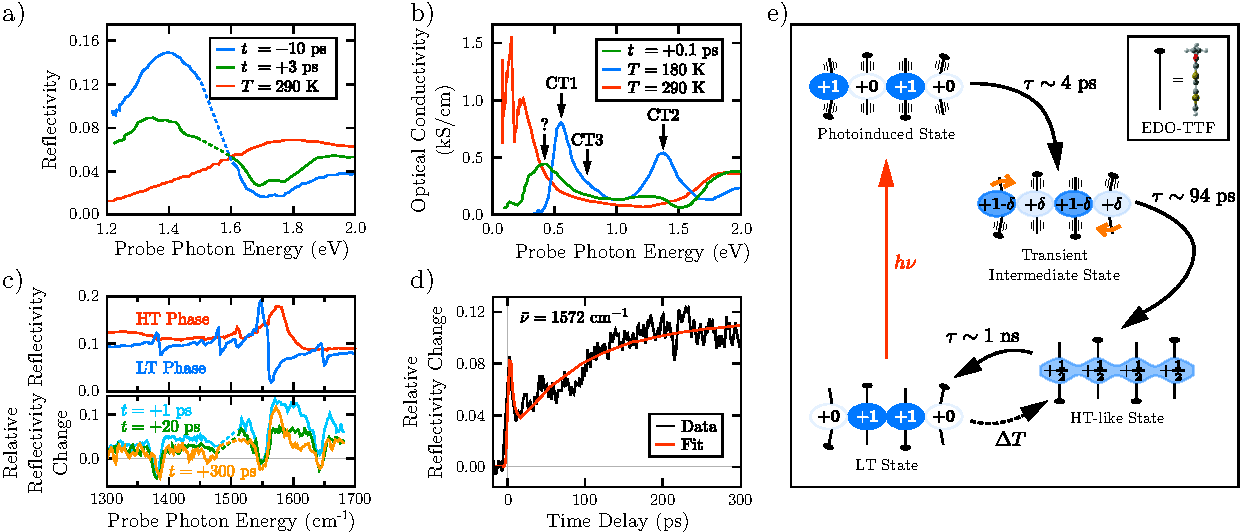
\includegraphics[width = \textwidth]{Figures/fig_EDO_time-resolved.pdf}
  \caption[Ultrafast time-resolved pump-probe spectroscopy in
  (EDO-TTF)\textsubscript{2}PF\textsubscript{6}.]{
  (EDO-TTF)\textsubscript{2}PF\textsubscript{6} crystals at low temperature
  are studied with ultrafast time-resolved pump-probe spectroscopy
  using a $800$-nm $120$-fs pump and different probes.
  (a)~With photons spanning the CT2~band, a collapse in reflectivity was observed,
  indicating photoinduced metallization of the insulator LT phase within a few hundred femtoseconds.
  (b)~With a broadband near-IR probe, the transient optical conductivity spectrum was reconstructed,
  enabling its assignment to a $(1010)$-type electronic state.
  (c)~In the mid-IR range, features associated with the C=C stretching modes are observed;
  (d)~their temporal evolution can be fitted to a three-level kinetic model.
  (e)~Schematic illustration of time evolution of the charge order and molecular structure
  following photoexcitation, as proposed in Ref.~\cite{Fukazawa2012}.
  Panels~(a)--(d) are adapted with permission from Refs.~\cite{Chollet2004, Onda2008, Fukazawa2012, Onda2014}
  respectively.
  }
  \label{fig: EDO-time-resolved}
\end{figure}
%
In 2004, Chollet et~al~\cite{Chollet2004} observed using time-resolved reflectivity spectroscopy that
the spectral features of a (EDO-TTF)\textsubscript{2}PF\textsubscript{6} crystal below $T_\text{MI}$
associated with its CT2 band oscillated and decreased dramatically within $3$~ps
being illuminated by a $800$-nm $120$-fs laser with photon energy ($1.55$~eV)
that is nearly resonant to the electronic transition itself (Fig.~\ref{fig: EDO-time-resolved}a).
%
This discovery suggests that the material underwent an ultrafast and reversible photoinduced
insulator--metal~(IM) phase transition and CO melting
when its $(1001)$ ground state is optically pumped to a $(2000)$ photoexcited state
which rapidly decays to the final state that is assumed to be metallic and HT-like.
%
However, the bandwidth of the reflectivity measurements ($1.2$--$2.0$~eV) was too narrow
to reconstruct the transient optical conductivity spectrum using the Kramers-Kronig relations%
\footnote{Dutch physicist Hendrik A. Kramers (1894--1952) and German physicist Ralph de~L. Kronig (1904--1995)
independently showed that the dispersive and absorptive properties of a medium are related from one to another and
can be calculated using a set of mathematical equations now known as
the Kramers-Kronig relations~\cite{Kronig1926, Kramers1927, KramersBook}.}
and characterize the short-lived photoinduced phase.
%
Later, Onda et~al~\cite{Onda2008} extended this experiment to a much wider range of the EM~spectrum
by measuring the photoinduced changes in reflectivity with a near-IR broadband probe
whose photon energies ranged from $0.069$ to $2.1$~eV.
As seen in Fig.~\ref{fig: EDO-time-resolved}b,
the reconstructed optical conductivity spectrum of at $t = +0.2$~ps is distinct from
that of either HT and LT phases, having lost the CT1 and CT2 bands and gained a new CT~band at $0.4$~eV.
These features thus characterize a heretofore unknown electronic state that
the authors were able to reproduce as a nonequilibrium $(1010)$ charge-disproportionate state
using a time-dependent model calculation based on a ex-PHH Hamiltonian.
%
Fukazawa et~al~\cite{Fukazawa2012} further expanded on these PIPT~study
by monitoring the differential reflectivity signal of the photoexcited state
first at select near-IR probe energies up to $t = +1000$~ps with $3$~ps pulses.
%
It was found that, for $t > 3$~ps, the spectral features evolve away from
those of the previously identified photoinduced $(1010)$ state to
those similar to the thermally induced metallic state.
%
This suggests that a metastable HT-like intermediate forms as the initially photoexcited state
relaxes back to the $(1001)$ ground state of the LT phase.
%
To follow the charge- and lattice-coupled dynamics that occur during this photocycle,
Fukazawa et~al also measured the transient reflectivity of the sample in the mid-IR range ($1300$--$1700$~cm$^{-1}$)
that spanned the absorption bands of several charge-sensitive EDO-TTF vibrational modes.
%
As in Ref.~\cite{Drozdova2004}, these modes --- $\nu_\alpha, \nu_\beta, \nu_\gamma$ ---
are stretching vibrations of C=C bonds that lengthen when the molecule becomes more positively charged.
%
Here, it was observed that excited state reflectivity at the vibrational bands
associated with the metallic state does appear eventually,
suggesting a process of molecular and/or lattice deformation (see Fig.~\ref{fig: EDO-time-resolved}c)
%
However, this feature does not appear concomitantly with the onset of ground state bleach,
refuting the earlier conclusion in Ref.~\cite{Chollet2004} that
PIPT occurs and is completed within a few picoseconds.
%
Instead, fitting of temporal profiles in the transient vibrational spectra
supports the idea of a slower process of metallization with a time constant of $94$~ps that is preceded by
an unspecific vibrationally hot transient state in the midst of charge disproportionation and
structural reorganization (see Fig.~\ref{fig: EDO-time-resolved}d and e).

% modifying inter- and intra-stack coupling.
% Susceptible to Peierls mechanism -> transition to insulator at low temperature
% to reduce Mott-Hubbard mechanism -> more polarizable atoms to reduce Coulomb repulsion and increase electron donation
% to reduce Peierls mechanism -> higher pressure -> increase intrastack overlap
% end-groups to reduce interstack coupling

\section{Mapping Molecular Motions in (EDO-TTF)\textsubscript{2}PF\textsubscript{6}}
\label{sec: UED-EDOPF6}

Altogether, the static and time-resolved measurements made on (EDO-TTF)\textsubscript{2}PF\textsubscript{6}
suggests a highly efficient and ultrafast photoinduced IM~phase transition at low temperature
that involves an unique convergence of several collective phenomena:
charge ordering, Peierls instability, bond ordering, and anion ordering.
%
To probe directly the structural evolution associated with this complex process,
the hybrid DC-RF UED setup described in Sec.~\ref{sec: UED-setup} is employed
and the resulting work is described as follows.

\subsection{Methods}

% The sample
Molecules of EDO-TTF are synthesized according to Ref.~\cite{Meziere2000} and
the PF\textsubscript{6} salt is formed through a process of electrochemical oxidation
and crystallization in the presence of tetrabutylammonium hexafluorophosphate
([N(C\textsubscript{4}H\textsubscript{9})\textsubscript{4}]\textsubscript{2}PF\textsubscript{6})
in ethanol~\cite{BechgaardJerome1982, Ota2002}.
%
As seen in Fig.~\ref{fig: EDO-samplePF6}a,
the resulting millimeter-sized black lustrous crystals of (EDO-TTF)\textsubscript{2}PF\textsubscript{6}
are mounted on blocks of epoxy resin in preparation for ultramicrotomy~\cite{UltramicrotomyManual}.
%
\begin{figure}[ht!]
  \centering
  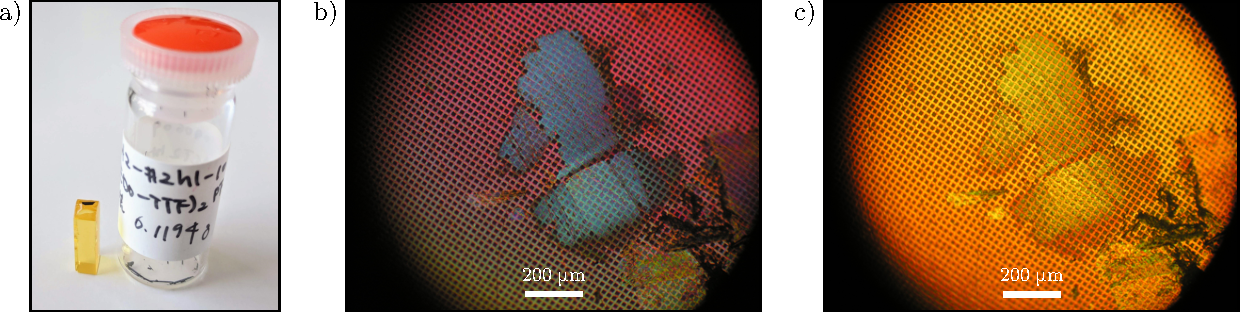
\includegraphics[width = \textwidth]{Figures/fig_EDO_samplePF6.pdf}
  \caption[Photos of (EDO-TTF)\textsubscript{2}PF\textsubscript{6} crystals and ultramicrotomed samples.]{
  (a) Black (EDO-TTF)\textsubscript{2}PF\textsubscript{6} crystals in a sample vial, next to
  a block of epoxy resin with a singular crystal embedded on top in preparation for ultramicrotomy.
  A 100-nm thick crystal section mounted on a TEM copper mesh grid in an optical microscope
  under different polarized illumination: (b) parallel and (c) orthogonal to the EDO-TTF stacking axis.
  The photos are courtesy of Dr.~Cheng Lu.
  }
  \label{fig: EDO-samplePF6}
\end{figure}
%
Slices --- 500~$\unslant\mu$m $\times$ 500~$\unslant\mu$m $\times$ 100~nm in size --- are cleaved roughly
parallel to the $\boldsymbol{a}_1$ $\times$ $\boldsymbol{a}_2$ crystal plane
and scooped from the water surface using standard TEM copper mesh grids
with different types of support membranes.
%
These samples are then observed in an optical microscope under illumination of varying polarization
to confirm the dichroism expected of (EDO-TTF)\textsubscript{2}PF\textsubscript{6}:
absorptive to light polarized parallel to the stacking axis, transmissive otherwise.
This behaviour is seen in Fig.~\ref{fig: EDO-samplePF6}b and c as the colour of a crystal slice
disappears as the polarization is rotated by $90^\circ$.
%
Finally, the mesh-mounted crystal slices are placed at the focal position of the UED setup,
depressurized, and cooled to the LT phase by connecting the sample holder to
a home-built liquid-nitrogen cold finger.
As measured by a calibrated platinum thermistor, their equilibrium temperature is found to be $(230 \pm 5)$~K,
well below $T_\text{MI} = 279$~K.

% Laser condition
To trigger the PIPT of (EDO-TTF)\textsubscript{2}PF\textsubscript{6},
the $60$-fs, $800$-nm output of the Ti:Sapph laser system is focused onto a free-standing section
of the sample, with a spot size of $(400 \pm 20)$~$\unslant\mu$m, a repetition rate of 10~Hz,
and a pulse energy of $2.0$~$\unslant\mu$J.
%
Although the pump wavelength is not perfectly resonant with the CT2 band ($897$~nm),
the absorption feature is sufficiently broad that PIPT is still triggered~\cite{Chollet2004, Onda2008}.
%
To maximize absorption, the pump polarization is linear and
aligned with the transition dipole moment of the CT2 band,
which is parallel to the stacking axis of the (EDO-TTF)\textsubscript{2}PF\textsubscript{6} molecules.
%
The pump transmittance of the sample at normal incidence is measured to be $(66 \pm 2)$~\% at 230~K
and $(93 \pm 2)$~\% at 295~K.
Given the incident pulse fluence (0.55~mJ/cm$^2$ or 0.22~$\unslant[-.15]\gamma$/\AA$^2$),
the excitation fraction of 0.08~$\unslant[-.15]\gamma$ per unit cell in the LT phase.
%
% UED conditions
The probe is a beam of $40$-fC (ca.~$2.5 \times 10^5$~e$^{-}$) electron pulses
with a spot size of $(280 \pm 20)$~$\unslant\mu$m FWHM that is centered on the pump spot.
As measured in Ref.~\cite{Gao2012}, the overall IRF is $(430 \pm 75)$~fs FWHM.

% Damage
\begin{figure}[ht!]
  \centering
  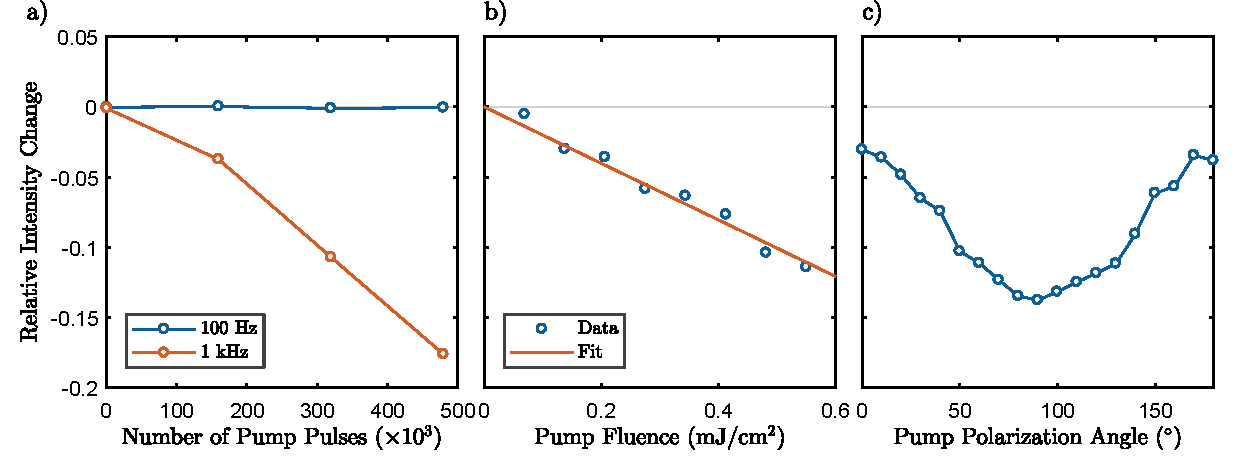
\includegraphics[width = \textwidth]{Figures/fig_EDO_control.pdf}
  \caption[UED signal dependence on the pump-laser repetition rate, fluence, and polarization angle.]{
  Controlled experiments are performed for validating the integrity of the sample.
  Changes in the intensity of $(h_1 h_2 h_3)$ diffraction spots with odd-$h_2$
  --- present in the LT phase and absent in the HT phase ---
  are monitored as a function of different pump laser parameters:
  (a)~repetition rate, (b)~fluence, and (c)~polarization angle.
  Panel~(a) shows sample integrity/damage under low/high repetition rate;
  Panel~(b), linear sample response to optical pumping;
  Panel~(c), nominal dichroism associated with 800-nm absorption at the CT2 band of (EDO-TTF)\textsubscript{2}PF\textsubscript{6}~\cite{Drozdova2004}.
  }
  \label{fig: EDO-control}
\end{figure}
%
In Sec.~\ref{sec: electrons-vs-xrays}, it is demonstrated that
time-resolved pump-probe experiments can exposed samples to damaging levels of radiation,
potentially leading to spurious results.
%
Here, controlled experiments are collected to validate
the UED measurements on (EDO-TTF)\textsubscript{2}PF\textsubscript{6}.
As seen in Fig.~\ref{fig: EDO-control}, the intensity of select diffraction spots
are monitored under different pump laser conditions.
Panel~(a) shows that photoexcitation at the 1-kHz repetition rate of the laser system causes
the diffraction features to decay, suggesting that
heat deposited by the pump laser is accumulating over laser pulses and
the sample is being progressively damaged.
%
Reducing the repetition rate to 100~Hz prevents this problem,
albeit at the cost of much longer experiment time,
by allowing enough time in between laser pulses for the sample to dissipate the thermal energy radiatively
and/or through conduction to the supporting copper mesh.
%
Panel~(b) shows the dependence of the intensity of diffraction spots characteristic of the LT phase
(at $t = +1$~ns) on the incident pump laser fluence. From the linearity of this trace up to $0.55$~mJ/cm$^2$
(0.22~$\unslant[-.15]\gamma$/\AA$^2$), it is clear that no photodamage has occurred.
%
Panel~(c) shows the intensity of the LT diffraction spots (at $t = +100$~ps)
as a function of the polarization angle of the pump laser.
As expected, a maximum and minimum separated by 90$^{\circ}$ is observed.
Per Malus'~law,%
\footnote{French engineer \'{E}tienne-Louis Malus (1775--1812) discovered that
transmission of polarized light through a dichroic material varies as $\cos^2(\theta)$,
where $\theta$ is the polarization angle of the light~\cite{CollettBook}.}
the absorption of (EDO-TTF)\textsubscript{2}PF\textsubscript{6}
via its CT2 band is maximal when the polarization of the incident light is parallel to
the stacking axis of the EDO-TTF molecules, and minimal otherwise~\cite{Drozdova2004}.
Indeed, the 800-nm photons of the pump laser have targeted the correct electronic excitation
to initiate the desired photoinduced dynamics.

% Unit cell definition
\begin{figure}[ht!]
  \centering
  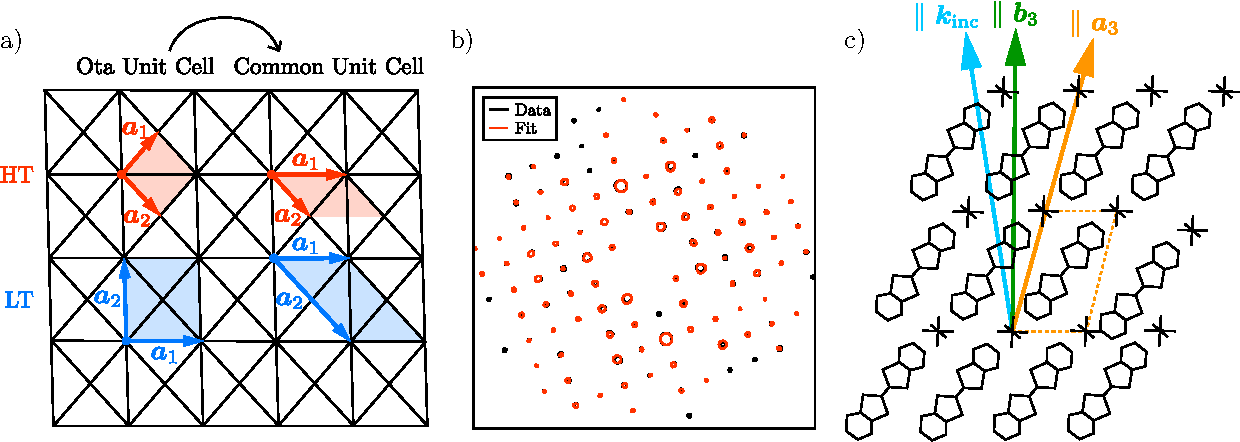
\includegraphics[width = \textwidth]{Figures/fig_EDO_unitcell_ori.pdf}
  \caption[Indexing of diffraction pattern and refinement of crystal orientation.]{
  Definition of crystallographic information.
  (a) A new unit cell, `common' to both LT and HT phases, is generated from symmetry transformation
  of the one published by Ota et~al~\cite{Ota2002}.
  (b) The indexing of the measured diffraction pattern, here represented by intensity contours,
  are determined by calculating simulated structure factors and fitting these values to the observed ones.
  (c) The orientation of the incident direction of the electron beam $\boldsymbol{k}_\text{inc}$
  is shown in relation to the real lattice vectors $\boldsymbol{a}_3$
  and its reciprocal counterpart $\boldsymbol{b}_3$.
  }
  \label{fig: EDO-unitcell-ori}
\end{figure}
%
In the present experiment, diffraction patterns are compared with each other
--- LT versus HT and pump-off versus pump-on --- as a mean to follow the changes in molecular structure
associated with the static and photoinduced phase transition.
%
As such, an indexing scheme common to both patterns is necessary.
%
However, the unit cells chosen by Ota et~al in their publication~\cite{Ota2002} are not totally overlapping
despite structures being in the same P$\overline{1}$ space group (Fig.~\ref{fig: EDO-unitcell-ori}a).
%
Thus, a new pair of unit cells, herein labeled `common' (as opposed to `Ota'), is defined as follows:
%
\begin{equation}
  \begin{aligned}
    (\boldsymbol{a}_{1, \text{HT}}, \boldsymbol{a}_{2, \text{HT}}, \boldsymbol{a}_{2, \text{HT}})
      & \rightarrow (\boldsymbol{a}_{1, \text{HT}} + \boldsymbol{a}_{2, \text{HT}},
        \boldsymbol{a}_{2, \text{HT}},
        \boldsymbol{a}_{3, \text{HT}}) \\
    (\boldsymbol{a}_{1, \text{LT}}, \boldsymbol{a}_{2, \text{LT}}, \boldsymbol{a}_{3, \text{LT}})
      & \rightarrow (\boldsymbol{a}_{1, \text{LT}},
        \boldsymbol{a}_{1, \text{LT}} - \boldsymbol{a}_{2, \text{LT}},
        - \boldsymbol{a}_{3, \text{LT}})
  \end{aligned}
\end{equation}
%
The resulting unit cells share similar lattice constants and angles,
with the exception of the length of $\boldsymbol{a}_2$
which is now aligned with the stacking axis of the EDO-TTF molecules.

% Indexing and orientation refinement
There are inherent uncertainties to the crystal orientation of the sample.
These stem from imperfect cleaving of the crystal during sample preparation
to misalignment of the sample holder with respect to the incident direction of the electron beam.
%
Since this quantity is necessary for the indexing and further analysis of the measured diffraction patterns,
an automatic procedure is set up to simulate the partial intensities that constitute a diffraction spot
for any arbitrary crystal orientation and then find the best fit to the observed values.
%
The details are described in Sec.~\ref{sec: UED-data-analysis-1} and
the results are shown in Figs.~\ref{fig: EDO-unitcell-ori}b and c.

The optimum orientation for the diffraction pattern of the LT and HT phases
are determined to be $[ u_1, u_2, u_3 ] = [-0.675, 0.600, 1.000]$ and
$[-0.640, 0.266, 1.000]$ respectively.
%
These two directions agree to about $1^\circ$ when both unit cells are placed
within the same Cartesian coordinate system ($\hat{\boldsymbol{x}} \parallel \boldsymbol{a}_1$
and $\hat{\boldsymbol{z}} \parallel \boldsymbol{a}_1 \times \boldsymbol{a}_2$).
%
The R-factor%
\footnote{The R-factor is a measure of agreement between the structure factor values
calculated from a crystallographic model and those which are experimentally observed;
it is defined as
$R = \frac{\sum \limits _j \left| |F_\text{sim}(\boldsymbol{q}_j)| - |F_\text{exp}(\boldsymbol{q}_j)| \right|}{\sum \limits _j \left| F_\text{exp}(\boldsymbol{q}_j) \right|}$.}
is calculated to be $35.2$~\% and $40.8$~\% for the LT and HT phases respectively.
Although these values are much higher than what is expected for single-crystal XRD,
they are typical for electron diffraction~\cite{ZouBook} and indicate reasonable agreement
between the observed diffraction intensities and those simulated using the present diffraction model
and the published crystal structures.

\begin{table}[ht!]
  \centering
  {\renewcommand{\arraystretch}{1.5}
  \begin{tabular}{ c c c c c c c }
    \toprule
    Phases & $a_1$ (\AA)  & $a_2$ (\AA)  & $a_3$ (\AA)  & $\alpha_{23}$ ($^{\circ}$) & $\alpha_{31}$ ($^{\circ}$) & $\alpha_{12}$ ($^{\circ}$) \\
    \midrule
    HT & $9.597$ & $7.343$ & $11.948$ & $93.42$ & $81.58$ & $48.05$ \\
    LT & $9.822$ & $14.803$ & $11.487$ & $92.72$ & $80.87$ & $47.99$ \\
    \bottomrule
  \end{tabular}
  }
  \caption{Lattice parameters of the `common' unit cell for the phases of (EDO-TTF)\textsubscript{2}PF\textsubscript{6}.}
  \label{tab: EDO-unitcell}
\end{table}


\subsection{Experimental Results and Discussions}
\label{sec: UED-EDO-Results}

In Panels a and b of Fig.~\ref{fig: EDO-LTHT}, the electron diffraction pattern of
the (EDO-TTF)\textsubscript{2}PF\textsubscript{6} in the LT and HT phases are shown.
As it can be seen in the difference image (Fig.~\ref{fig: EDO-LTHT}c),
there is a conspicuous appearance of a family of diffraction spots in the HT image.
Under the indexing scheme described earlier, all these spots have a Miller index $(h_1 h_2 h_3)$
where $h_2$ is an odd integer, clearly indicative of the unit-cell doubling along the stacking axis
that is associated with the IM~phase transition.
%
Thus, it is confirmed that the diffraction intensities observable in this crystal orientation
are sensitive to the structural changes relevant to PIPT.
%
\begin{figure}[ht!]
  \centering
  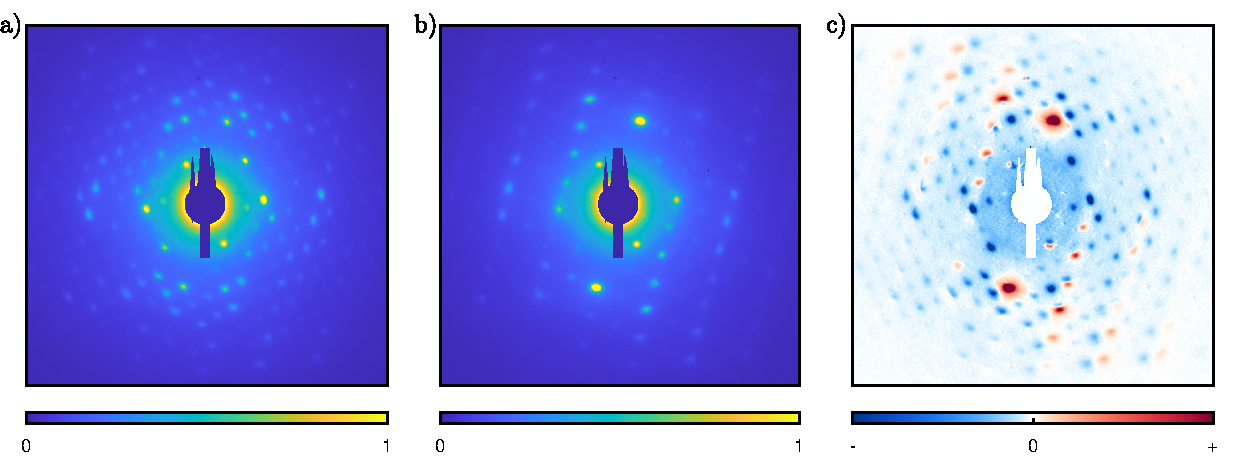
\includegraphics[width = \textwidth]{Figures/fig_EDO_LTHT.pdf}
  \caption[Static electron diffraction patterns of (EDO-TTF)\textsubscript{2}PF\textsubscript{6}
  above and below $T_\text{IM}$.]{
    Static electron diffraction data of the (EDO-TTF)\textsubscript{2}PF\textsubscript{6} samples
    are taken at (a) low temperature ($T = 230$~K) and (b) ambient temperature ($T = 295$~K),
    below and above $T_\text{IM}$ respectively.
    Panel (c) shows the difference between these two patterns.
  }
  \label{fig: EDO-LTHT}
\end{figure}

To monitor the photoinduced structural evolution of the molecular system,
pump-on and pump-off diffraction patterns are collected at different time delays.
From the difference images (Fig.~\ref{fig: EDO-TRresults}a),
a complex pattern of intensity changes is visible.
%
\begin{figure}[ht!]
  \centering
  \includegraphics[width = \textwidth]{Figures/fig_EDO_TRresults.pdf}
  \caption[Time-resolved UED data of (EDO-TTF)\textsubscript{2}PF\textsubscript{6}.]{
  Time-resolved UED data of (EDO-TTF)\textsubscript{2}PF\textsubscript{6}.
  (a) Difference images at different time points show the pattern of diffraction intensity changes
  associated with the structural dynamics that follows photoexcitation of the LT ground state;
  the difference image between the LT and HT phases is included on the far right to emphasize
  the similarity between the HT diffraction pattern and that observed at $t = +1$~ns.
  (b) Time traces for some selected diffraction spots are plotted on two timescales
  (from $-3.6$ to $+17$~ps; from $+17$ to $+500$~ps)
  to showcase the presence of fast and slow processes which are at work.
  }
  \label{fig: EDO-TRresults}
\end{figure}
%
The most succinct observation is the similarity between the $+1$~ns difference image and the one measured
across the thermal phase transition, immediately suggesting that the photoinduced structural dynamics ends
at a HT-like state.

Fig.~\ref{fig: EDO-TRresults}b gives the temporal evolution of the intensity of
some selected diffraction spots. From these time traces, two components is resolved:
a `fast' change on the order of a few picoseconds and a `slow' one that proceeds on the 100-ps timescale.
%
The former can be explained as the result of femtosecond optical excitation
altering the charge distribution within the EDO-TTF stack, modifying various intermolecular and intramolecular forces,
and driving coherent molecular motions.
%
The slow component is attributed to uncorrelated motions that provide an ensemble-averaged picture
of the structural evolution, i.e.~a thermal relaxation process that brings the molecular system
to the final HT-like state~\cite{Fukazawa2012}.
%
In addition, oscillations with a period of a few hundred picoseconds are apparent after $+100$~ps
(right side of Fig.~\ref{fig: EDO-TRresults}b);
they are likely a manifestation of the transfer of heat to the lattice
as strain waves are generated~\cite{Harb2009, Maher-thesis}.
%
Finally, a plateau can be readily seen on the ultrafast timescale (left side of Fig.~\ref{fig: EDO-TRresults}b)
wherein the intensity of all diffraction spots remains unchanging over time delays between $+3$ and $+10$~ps.
This behaviour indicates the presence of a transient intermediate state~(TIS)
along the pathway of the PIPT process.
Given that optical studies give evidence to large charge fluctuations
prevailing in this time span~\cite{Onda2008, Fukazawa2012},
it is plausible that the effective intermolecular forces are screened and
the structure of the molecular system is therefore transiently locked.

To obtain a time-dependent map of the relevant molecular motions driving
the IM~phase transition and the intervening formation of the TIS structure,
a structural refinement scheme based on a parameterized molecular model is employed.
The details of this general method are described in Sec.~\ref{sec: UED-data-analysis-3}
and it is applied to (EDO-TTF)\textsubscript{2}PF\textsubscript{6} as follows.

% Spot restriction and molecular model
The set of diffraction spots used in the refinement calculations is restricted to those
which are proximate to the Ewald sphere and do not contain contribution from multiple relrods.
%
In addition, the end-point crystal structures of the linear interpolation in Eq.~\eqref{eq: linear-model}
are chosen to be those of the LT and HT phases respectively.
%
To construct the candidate structures for the time-dependent optimization,
inversion symmetry is assumed to be conserved and
the two (EDO-TTF)\textsubscript{2}PF\textsubscript{6} molecules in the unit cell
are divided by symmetric nonequivalency into three dynamical groups which display distinct motions.
%
As seen in Fig.~\ref{fig: EDO-movie}a,
the first group ($\xi_1$) is composed of atoms of the bent neutral EDO-TTF molecules
whose IM~displacement $\Delta \bscriptr_{i} = \bscriptr_{i, \text{HT}} - \bscriptr_{i, \text{LT}}$
is primarily a flattening motion;
%
the second group ($\xi_2$), the atoms of the PF\textsubscript{6} counterions that rotate and
move to the nearest point of symmetry;
%
the last group ($\xi_3$), the atoms of the flat monovalent EDO-TTF molecules
which slide perpendicularly to the stacking axis
and become translationally equivalent to the atoms of the first group;
%
\begin{figure}[ht!]
  \centering
  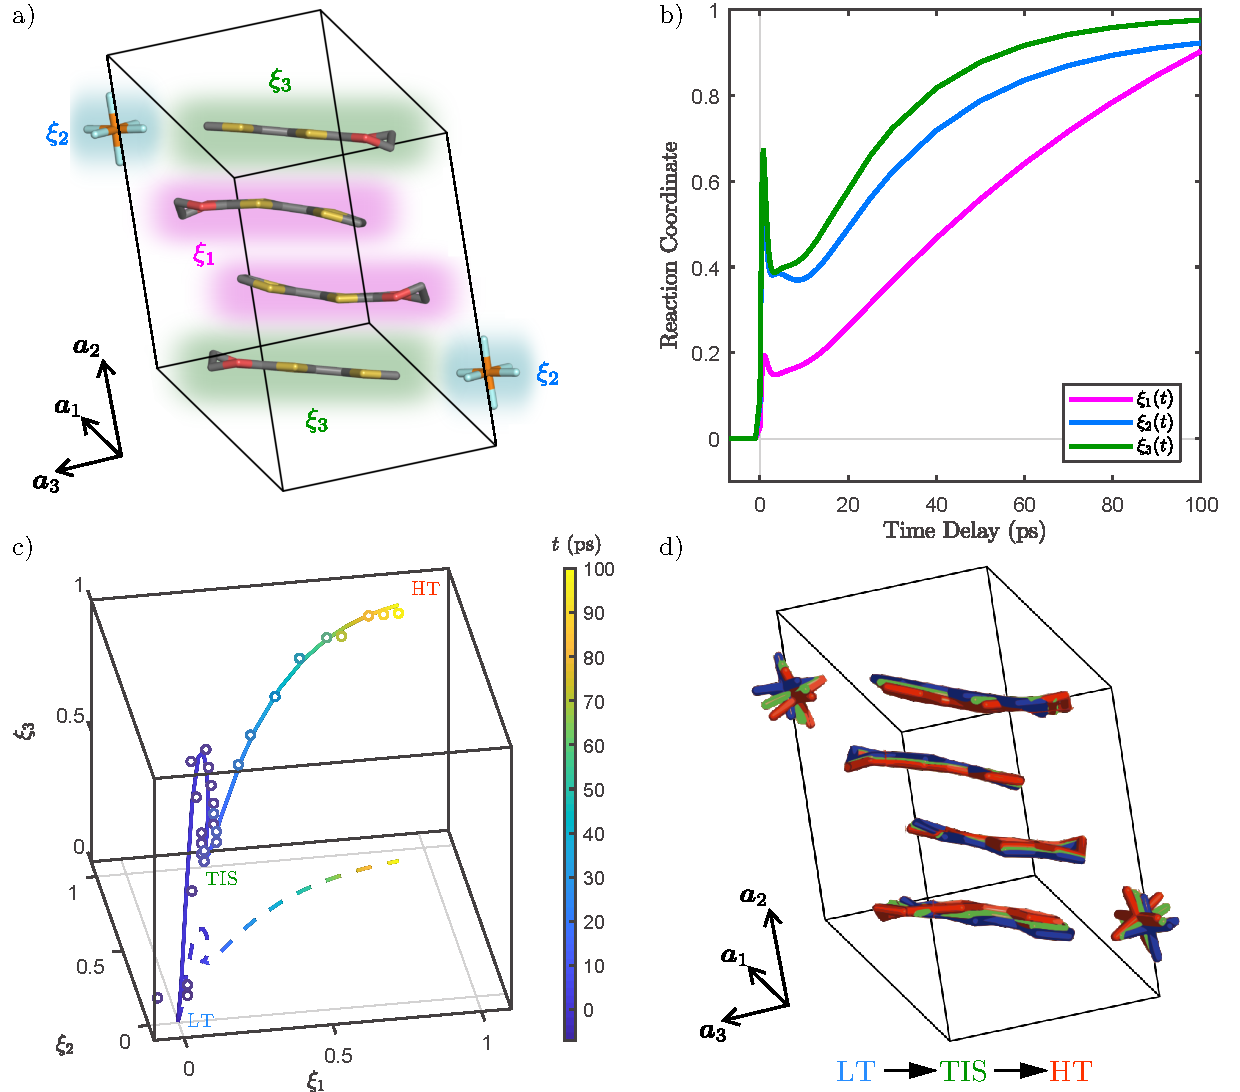
\includegraphics[width = \textwidth]{Figures/fig_EDO_movie.pdf}
  \caption[Structural dynamics of (EDO-TTF)\textsubscript{2}PF\textsubscript{6} in configuration space.]{
  Structural dynamics of (EDO-TTF)\textsubscript{2}PF\textsubscript{6} in configuration space.
  Refinement of the UED data is performed by
  (a) partitioning the atoms of the unit cell into three dynamical groups (highlighted in magenta, cyan, and green) and
  (b) optimizing the goodness-of-fit $P$ between the measured structural factors and the simulated ones
  over the associated reaction coordinates $\xi_1, \xi_2, \xi_3$ for each time point $t$
  (lines shown are the multiexponential fits).
  The result is (c) a reaction pathway through configuration space that fully maps
  the molecular displacements of (EDO-TTF)\textsubscript{2}PF\textsubscript{6}
  as it goes from (d) the LT state to TIS and finally a HT-like state
  (coloured respectively in blue, green, and red).
  %
  Circles are the independently optimized structures;
  the solid lines are the multiexponential fits; the dashed line is a two-dimensional projection.
  Panel (a) is courtesy of Dr.~Alexander Marx.
  }
  \label{fig: EDO-movie}
\end{figure}
%
This approach reduces the structure refinement of each pattern of diffraction intensity changes
from a problem with $3N_\text{at} - 6$ variables to one with only $3$
while still capturing most of the physics without nonsensical results caused by overfitting.

% Excitation fraction
To determine the value of the excitation fraction~$\eta_\text{exc}$
(the fraction of unit cells engaging in the PIPT process),
it is assumed that the photoexcited molecular system has fully thermalized into a HT-like state
by $t = +1$~ns and little residual thermal stress remains;
Since $F_\text{on}(\infty, \boldsymbol{q}) \approx F_\text{on}(+1 \text{ ns})$,
$\eta_\text{exc}$ is calculated to be about $10.3$~\% using Eq.~\eqref{eq: nexc},
i.e.~the equation of Coppens et~al in the low-excitation limit~\cite{CoppensBook, Coppens1998, Coppens2005}.
%
These are fair assumptions to be made here, considering that the acoustic oscillations have damped away by $t > +500$~ps,
the estimated temperature increase is less than $50$~K, and the effect of residual stress is minimized
for reflections satisfying the Laue-Bragg condition~\cite{Harb2009}.
%
Also, from optical reflectivity and in situ optical transmission measurements,
a similar value (ca.~$8$~\%) is estimated using Eq.~\eqref{eq: nexc-optical}
for the fraction of ground unit cells which are photoexcited by the pump laser pulse.
%
Furthermore, optimization of the goodness-of-fit~$P$ as a function of $\eta_\text{exc}$ and
time delay~$t$ during the structural refinement process shows a maximum of ca.~$10$~\%
that persists over the interval of 0 to $+10$~ps.
%
Given the consistency of these independent evaluations of $\eta_\text{exc}$,
it is clear that the initial excitonic correlation length only extends over about one LT unit cell
and only local structural changes are promoted with a photoconversion efficiency of about unity.
%
This result runs counter to the observation of highly cooperative `photo-domino effect' by
Chollet et~al~\cite{Chollet2004} wherein an excitation fraction of $0.7$~\%
(one absorbed photons for every 142 LT unit cells) supposedly lead to the IM~conversion fraction of $50$~\% and
a photoconversion efficiency of 71 times unity.
%
Onda et~al~\cite{Onda2014} states that the discrepancy is explained by
the incorrect assumption in the latter work that the IM~conversion fraction can be simply and directly estimated by
the change in the reflectivity of the CT2 band at $t = +3$~ps.

In Fig.~\ref{fig: EDO-movie}b, the result of the structure refinement is shown.
For each time delay $t$, a set of optimized reaction coordinates $(\xi_1, \xi_2, \xi_3)$ is obtained;
each coordinate can then be fitted by a multiexponential function
that is based on the three-level rate model
proposed by Fukazawa et~al~\cite{Fukazawa2012}:
%
\begin{equation}
  \begin{aligned}
    f(t) & =
      \left[ H(t) \left(
        c_1 \left( \mathrm{e}^{-k_2 t} - \mathrm{e}^{-k_1 t} \right) +
        c_2 \left( \mathrm{e}^{-k_4 t} - \mathrm{e}^{-k_3 t} \right) +
        c_3 \left( 1 - \mathrm{e}^{-k_5 t} \right)
        \right) \right] \ast \text{IRF}(t)
  \end{aligned}
\end{equation}
%
where $H(t)$ is the Heaviside function,
$\textrm{IRF}(t) = \mathrm{e}^{- \frac{1}{2} t^2/\tau_\text{IRF}^2}$ is
the instrument response function with $\tau_\text{IRF}$ = $430$~fs, and
$k_i, c_j$ are the time constants and coefficients to be fitted.

Altogether, the fit results are shown in Tab.~\ref{tab: EDO-fit} and
a trajectory in $\boldsymbol{\xi}$-space can be plotted that represents the reaction pathway
taken by the molecular system following photoexcitation (see Fig.~\ref{fig: EDO-movie}c).
%
\begin{table}[ht!]
  \centering
  {\renewcommand{\arraystretch}{1.5}
  \begin{tabular}{ c c c c c c c c c }
    \toprule
      & $c_1$ & $c_2$ & $c_3$ & $\tau_{1}$ (ps) & $\tau_{2}$ (ps) & $\tau_{3}$ (ps) & $\tau_{4}$ (ps) & $\tau_{5}$ (ps) \\
    \midrule
    $\xi_1 (t)$ & $15.3$ & $6.9$ & $1.46$ & $0.70$ & $0.70$ & $3.4$ & $3.6$ & $100$\\
    $\xi_2 (t)$ & $56.0$ & $1.0$ & $0.95$ & $0.49$ & $0.53$ & $2.8$ & $3.2$ & $23$\\
    $\xi_3 (t)$ & $32.0$ & $6.0$ & $1.23$ & $0.44$ & $0.45$ & $2.0$ & $4.3$ & $28$\\
    \bottomrule
  \end{tabular}
  }
  \caption{Values of the multiexponential model fitted for
  the reaction coordinates~$\xi_i$ of (EDO-TTF)\textsubscript{2}PF\textsubscript{6}.}
  \label{tab: EDO-fit}
\end{table}
%
It can be clearly seen that
the structure of (EDO-TTF)\textsubscript{2}PF\textsubscript{6} evolves from the  LT state
($\boldsymbol{\xi}(t = 0) = (0, 0, 0)$) through concerted atomic motions
towards the HT state ($\boldsymbol{\xi}(t > +100 \text{ ps}) = (1, 1, 1)$)
with a brief, few-picosecond pit stop at the TIS
($\boldsymbol{\xi}(t \sim +3 \text{ ps}) = (0.15, 0.38, 0.40)$).
%
From the relative values and timing of the reaction coordinates,
it is observed that the motions of the flat monovalent EDO-TTF molecules and
the PF\textsubscript{6} counterions are correlated.
This suggests that optical excitation mostly drives the formation of the TIS through these modes
while the bent neutral donor molecules are unchanged.
%
Furthermore, the overshooting of these two coordinates at $t = +1$~ps is indicative
of an overdamped half-cycle motion.
%
These time-dependent correlations,
in addition to the close proximity of the counterions to the charged donors,
provide evidence for the role of steric effects --- short-range repulsive interactions ---
are also important in the crystalline order and positioning of the molecules.


\subsection{Summary and Conclusions}

From Onda et~al~\cite{Onda2008},
the ex-PHH model (see App.~\ref{ap: exPHH})
can reproduce the spectral signature of the $(0101)$ excited state
by including off-site Coulomb repulsion and electron-phonon interactions that
modulate the site energies via anion displacements.
%
The UED results herein support this description and correspondingly indicate that
the motion of the PF\textsubscript{6} counterions is an important component in the evolution of
the electronically excited LT and the formation of the TIS structures.
%
This is a curious development given that
PF\textsubscript{6}$^-$ is mostly known for its chemical stability and weak coordinating ability~\cite{Strauss1993}
and its intended role in (EDO-TTF)\textsubscript{2}PF\textsubscript{6}
probably was to electrically balance the positive charges and
passively spectate the physics of the molecular system.
%
Indeed, this connection between the counterions and the charge fluctuations leading to PIPT
suggests that they ought to be targeted for chemical modification
if the electronic properties of this crystal are to be taken controlled.
%
This approach to molecular design would be similar to the anion substitution in (TMTSF)\textsubscript{2}X
that led to the synthesis of the first ambient-pressure
organic superconductor~\cite{Bechgaard1980, Bechgaard1981}.
%
In contrast, the small relative amplitude of the flattening of the neutral EDO-TTF molecules
in the formation of the TIS questions the relevance of the simple bending--flattening type
of distortion mode to the charge disproportionation.
%
Future UED experiments can focus on different sample orientations with improved spatial resolution
and apply more general refinement methods for real-space reconstruction;
ab initio electronic calculations would link the resolved dynamics of the molecular structure with
the evolution of the charge distribution.


\section{Counterion Effect in (EDO-TTF)\textsubscript{2}SbF\textsubscript{6}}
\label{sec: UED-EDOSbF6}

\begin{figure}[ht!]
  \centering
  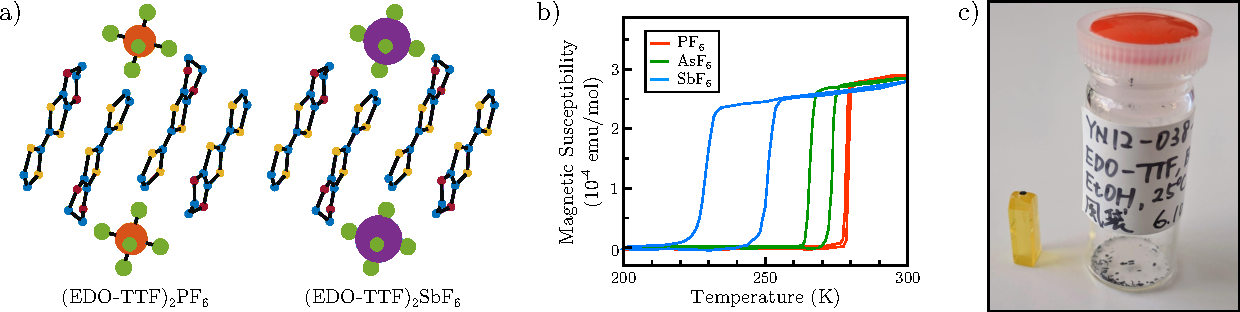
\includegraphics[width = \textwidth]{Figures/fig_EDOSb_sample.pdf}
  \caption[Overview of (EDO-TTF)\textsubscript{2}SbF\textsubscript{6}.]{
  Overview of (EDO-TTF)\textsubscript{2}SbF\textsubscript{6}.
  (a) (EDO-TTF)\textsubscript{2}PF\textsubscript{6} and (EDO-TTF)\textsubscript{2}SbF\textsubscript{6}
  are isostructural in both LT and HT phases.
  (b) All three hexafluoropnictate derivatives of (EDO-TTF)\textsubscript{2}X
  exhibit similar MI~phase transitions but with decreasing $T_\text{MI}$ and
  increasing $\Delta T_\text{MI}$ for larger counterions.
  (c) Black (EDO-TTF)\textsubscript{2}SbF\textsubscript{6} crystals
  in a sample vial, next to   a block of epoxy resin with a singular crystal embedded
  on top in preparation for ultramicrotomy.
  Panel~(b) is adapted from Ref.~\cite{NakanoX} with permission
  from Prof.~Yoshiaki Nakano.
  }
  \label{fig: EDOSb-sample}
\end{figure}

Bechgaard-Fabre salts mostly assemble into similar crystal structures and
showcase a similar procession of ground states and collective phenomena
as different anions are substituted (see Fig.~\ref{fig: EDO-overview}d).
%
In particular, molecules of the (EDO-TTF)\textsubscript{2}X where X is one of the hexafluoropnictates
form isostructural crystals (Fig.~\ref{fig: EDOSb-sample}a) and
exhibit the same type of thermal MI~phase transition~\cite{Ota2002, Ota2003, Nakano2009}.
%
As seen in Fig.~\ref{fig: EDOSb-sample}b,
this phase transition is manifested by a sudden change in magnetic susceptibility of the material
as the Pauli paramagnetism%
\footnote{Named for Wolfgang Pauli (1900--1958) and his eponymous exclusion principle,
Pauli paramagnetism refers to the tendency of a `metal' to become weakly magnetized
under an applied magnetic field as its free electrons align with the field~\cite{Nobel1942, AshcroftBook}.}
of the metallic phase disappears in the insulator phase.

The parameters of the thermal MI~phase transition down this chemical series
are tabulated in Tab.~\ref{tab: EDO-TMI}.
Two trends can be seen as the size of the substituted pnictogen is increased:
a lowering of the transition temperature $T_\text{MI}$ and
a widening of the hysteresis loop $\Delta T_\text{MI}$~\cite{NakanoX}.
%
This observation, in addition to later work by Ota et~al~\cite{Ota2006}
where X is replaced by even larger anions ($\mathrm{GaCl_4^-}$ and $\mathrm{ReO_4^-}$),
suggests that large counterions can penetrate the EDO-TTF stack and
affect the electronic correlation relevant to the MI~phase transition.

Furthermore, it has been found spectroscopically that
the reverse insulator--metal phase transition can be triggered on the ultrafast timescale
in (EDO-TTF)\textsubscript{2}PF\textsubscript{6} by photoexcitation of
one of its charge-transfer bands~\cite{Chollet2004, Onda2008, Fukazawa2012}.
%
In the UED work described in Sec.~\ref{sec: UED-EDOPF6},
it has also been shown that the motion of the PF\textsubscript{6} counterions
plays a critical role in enabling this IM~transition by allowing the EDO-TTF molecules
to approach each other and interact, leading to the IM~transition.
%
However, no such PIPT could be detect in crystals of
(EDO-TTF)\textsubscript{2}SbF\textsubscript{6}~\cite{Lorenc2008, Servol2015}.
Time-resolved measurements of photoinduced changes in reflectivity only reveal
the excitation of some optical phonons followed by the formation of a local state
similar to the TIS of the PF\textsubscript{6} derivative, tentatively suggesting
that the larger counterion increases the distance between the EDO-TTF molecules
--- thus the unit-cell volume change~$\frac{\Delta V}{V_\text{HT}}$ (Tab.~\ref{tab: EDO-TMI})
and the resulting elastic energy cost necessary for the IM~transition ---
beyond what can be achieved during the photoinduced process~\cite{Servol2015}.
More details could be found in the doctoral theses in Refs.~\cite{Moisan-thesis, Kaszub-thesis}.

Therefore, a UED study on (EDO-TTF)\textsubscript{2}SbF\textsubscript{6} is called for
to follow-up on the previous work in Sec.~\ref{sec: UED-EDOPF6} and
offer direct structural confirmation of this `counterion effect.'
The resulting work is described as follows.

\begin{table}[ht!]
  \centering
    \begin{tabular}{c c c c c c}
      \toprule
      X & $T_{\text{MI}\downarrow}$~(K) & $T_{\text{MI}\uparrow}$~(K) & $T_\text{MI}$~(K) & $\Delta T_\text{MI}$~(K) & $\Delta V / V_\text{HT}$~(\%) \\
      \midrule
      PF\textsubscript{6}  & 278.5 & 279.5 & 279.0 & 1.0  & $-0.45$ \\
      AsF\textsubscript{6} & 268.0 & 273.5 & 270.8 & 5.5  & $-0.77$ \\
      SbF\textsubscript{6} & 235.0 & 249.0 & 242.0 & 14.0 & $-1.39$ \\
      \bottomrule
    \end{tabular}
  \caption{Hysteresis of the thermal MI~phase transition of different (EDO-TTF)\textsubscript{2}X.
    $T_{\text{MI}\downarrow}$ and $T_{\text{MI}\uparrow}$ are the transition temperature
    during the cooling and heating cycles respectively;
    $T_\text{MI} = \frac{1}{2} (T_{\text{MI}\downarrow} + T_{\text{MI}\uparrow})$ and
    $\Delta T_\text{MI} = T_{\text{MI}\uparrow} - T_{\text{MI}\downarrow}$.
    $\Delta V / V_\text{HT}$, where $\Delta V = V_\text{LT} - V_\text{HT}$,
    is the associated relative change in unit-cell volume at $T_\text{MI}$.
    The values herein are courtesy of Prof.~Yoshiaki Nakano~\cite{Nakano2008, NakanoX}.}
  \label{tab: EDO-TMI}
\end{table}

\subsection{Methods}

Single-crystals of (EDO-TTF)\textsubscript{2}SbF\textsubscript{6} are synthesized in
an analoguous manner as those of (EDO-TTF)\textsubscript{2}PF\textsubscript{6}
--- by electrocrystallization in ethanol.
The supporting electrolyte employed here is freshly purified (Bu\textsubscript{4}N)SbF\textsubscript{6}
whereas the original method used (EMI)SbF\textsubscript{6}
(EMI refers to 1-ethyl-3-methylimidazolium)~\cite{Maesato2009}.
%
These resulting dark crystals (see Fig.~\ref{fig: EDOSb-sample}c) are mounted on epoxy resin and
cleaved by ultramicrotomy into slices that are $150$~nm thick and typically $500$~$\unslant\mu$m across.
They are then scooped onto copper TEM meshes and mounted in the UED sample chamber.
%
During the UED measurements, the samples are kept at $180$~K using the liquid nitrogen cold finger,
well below the hysteresis loop of the MI~phase transition as seen in Fig.~\ref{fig: EDOSb-sample}b,
to ensure that they are fully in the LT phase ($T_\text{MI} = 242$~K and $\Delta T_\text{MI} = 14$~K).

The UED setup used herein is the same as the one in Sec.~\ref{sec: UED-EDOPF6} and
it is described in detail in Sec.~\ref{sec: UED-setup}.
%
In particular, the electron pulse duration is measured to be ca.~$300$~fs FWHM~\cite{Gao2013b}.
The pump laser has pulse duration of $60$~fs, centre wavelength of $800$~nm, and
a polarization that is adjusted to maximize sample absorption via the CT2 band.
The laser repetition rate is set at $10$~Hz to avoid damage of the sample caused by
cumulative heating.
%
At the sample position, the laser pulse energy is $0.63$~mJ/cm$^2$.
The excitation fraction $\eta_\text{exc}$ is determined to be ca.~$10$~\%
using the methods described in Sec.~\ref{sec: UED-EDO-Results}.

For data analysis, an approach different to that used for (EDO-TTF)\textsubscript{2}PF\textsubscript{6}
is adopted. By considering the similarity between broadband TA spectra and
time-resolved electron diffraction data, this work marks the first application of the SVD-based method described
in Sec.~\ref{sec: UED-data-analysis-2}.


\subsection{Experimental Results and Discussions}

\begin{figure}[ht!]
  \centering
  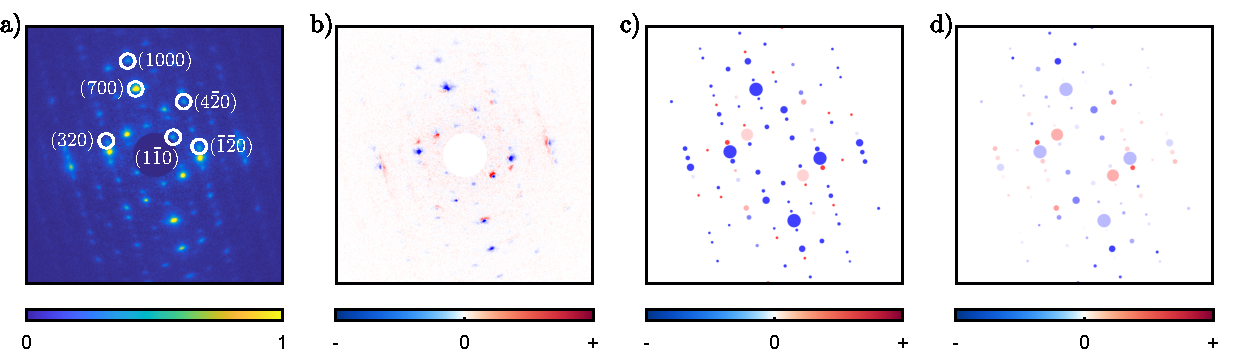
\includegraphics[width = \textwidth]{Figures/fig_EDOSb_UEDimages.pdf}
  \caption[Static and time-resolved electron diffraction patterns of
    (EDO-TTF)\textsubscript{2}SbF\textsubscript{6}.]{
    Electron diffraction patterns of (EDO-TTF)\textsubscript{2}SbF\textsubscript{6}:
    (a) static image of the LT phase ($T = 170$~K) with select spots circled for later reference;
    (b) difference image between the HT ($T = 300$~K) and LT phase;
    (c) scatter plot of the integrated intensity in Panel~(b);
    (d) scatter plot of the integrated intensity of the time-resolved difference image at $t = +100$~ps.
    %
    The size of the markers in Panels~(c) and (d) scales with the intensity of the diffraction spots
    and the face colour scales with the intensity difference.
  }
  \label{fig: EDOSb-UEDimages}
\end{figure}

The panels of Fig.~\ref{fig: EDOSb-UEDimages} show the electron diffraction patterns
of the (EDO-TTF)\textsubscript{2}SbF\textsubscript{6} samples in different states for comparison.
%
In Panel~(a), data for the LT phase is shown and a large number of diffraction spots can be seen.
They range from peaks close to the (000) transmitted beam to the high-order ones
near the edge of the camera sensor, suggesting a high degree of sample crystallinity and
a transverse beam coherence that is on the order of a few nanometers and thus sufficient to
atomically resolved changes to the crystal structure.

In Panel~(b), the difference image between the LT data and that collected when the sample is in
the HT phase ($T = 300$~K) is shown. Red and blue patches indicate the pattern of diffraction spots
that have respectively increased and decreased in intensity and/or have shifted in position within
reciprocal space. The former type of intensity changes is generally caused by atomic motions;
the latter would be associated with distortions in the shape or size of the unit cell.
Using the scattering equations described in Sec.~\ref{sec: UED-physics} and
refined HT and LT crystal information from Nakano et~al~\cite{NakanoX},
it is found that the observed thermal difference image is consistent with
the structural reorganization correlated with the MI~phase transition
of (EDO-TTF)\textsubscript{2}SbF\textsubscript{6}.

The scatter plots in Panels~(c) and (d) represent a reconstructed diffraction pattern where each marker
is sized and coloured respectively according to the diffraction spot intensity in the LT phase and
the relative change in intensity. As described in Sec.~\ref{sec: UED-data-analysis-1},
the position of the spots is fitted using Eq.~\eqref{eq: gaussian-spot} and
the intensity is calculated by integrating the detector counts in a circular region around the spot position.
%
In particular, Panel~(c) shows the changes in spot intensity that are caused by
the thermal IM~phase transition, and Panel~(d),
those that occur $100$~ps after photoexcitation of the CT2 band.
Clearly, the patterns do not match, thus indicating that the late-time molecular structure of
the photoinduced state of (EDO-TTF)\textsubscript{2}SbF\textsubscript{6} is not the same as
the structure of both the LT and HT states.
Furthermore, there is no discernible change in the position of the diffraction spots,
which is unsurprising since volume expansion of the unit cell is not expected
so soon after photoexcitation~\cite{Lorenc2009}
nor large enough to be resolvable presently~\cite{Gao2013}.

In Fig.~\ref{fig: EDOSb-UEDtraces}, the ultrafast structural dynamics
of both PF\textsubscript{6} and SbF\textsubscript{6} derivatives are compared.
%
The time traces for a number of diffraction spots are shown in Panels~(a) and (b);
these precise spots are selected to highlight the diversity of signals that can be
observed amongst the hundreds of features in the time-resolved diffraction patterns.
%
In particular, the PF\textsubscript{6} data is characterized by an sub-picosecond peak
that is followed by a few-picosecond plateau and then a slow evolution towards a HT-like state;
the Sb\textsubscript{6} data only shows bi-exponential dynamics on the order of tens of picoseconds
that terminates at a state structurally unlike either thermally accessible states.
%
Indeed, counterion substitution has a significant effect on the ultrafast structural reorganization
that occurs following photoexcitation.
%
\begin{figure}[ht!]
  \centering
  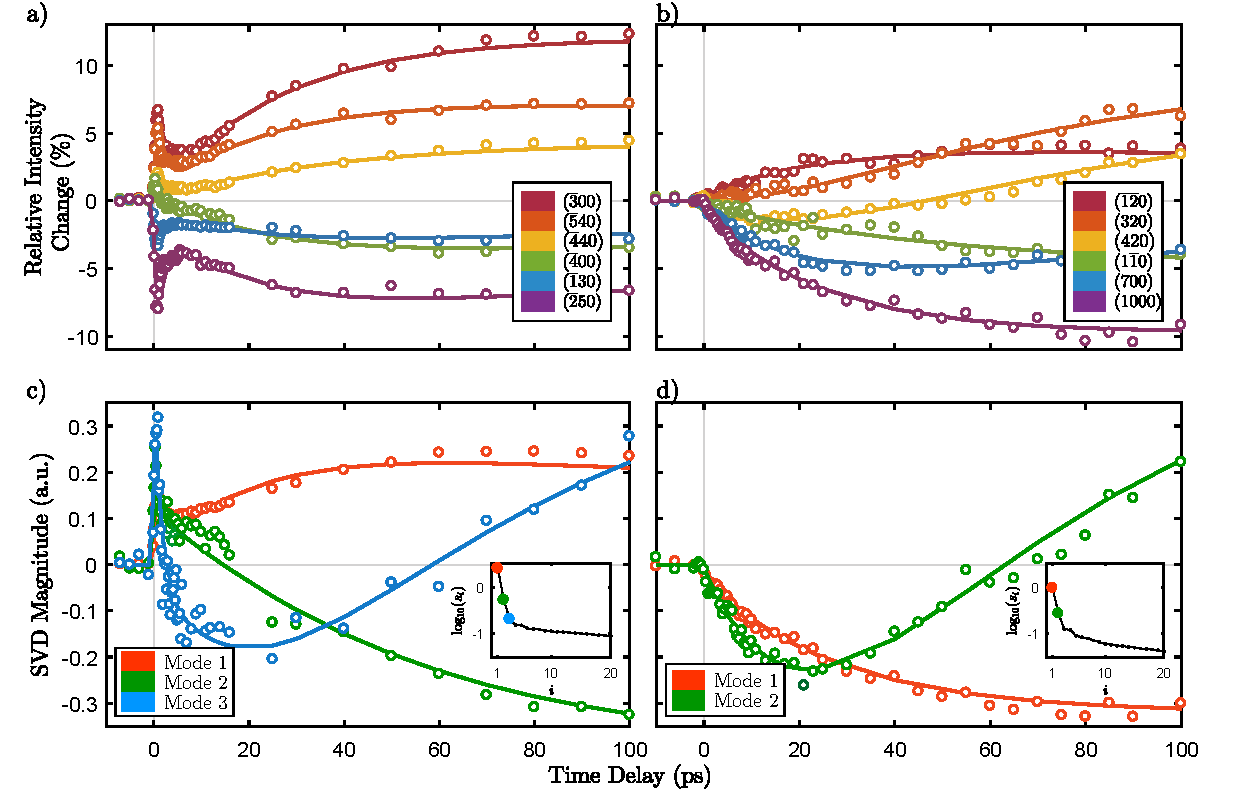
\includegraphics[width = \textwidth]{Figures/fig_EDOSb_UEDtraces.pdf}
  \caption[Time-resolved UED data of (EDO-TTF)\textsubscript{2}X
    (X = PF\textsubscript{6}, SbF\textsubscript{6}).]{
    Time-resolved UED data of (EDO-TTF)\textsubscript{2}X,
    where X = PF\textsubscript{6} (left panels) and SbF\textsubscript{6} (right panels).
    The top panels, (a) and (b), show the relative change in diffraction intensity
    at select diffraction spots following photoexcitation.
    The bottom panels, (c) and (d), show the principal right-singular vectors
    of the UED data; the insets are plots of $\log_{10} s_i$, where $s_i$ are the singular values
    sorted in descending order.
    The markers are measured values and the solid lines are lines of best fit
    from a global analysis.
  }
  \label{fig: EDOSb-UEDtraces}
\end{figure}

To better elucidate the influence of the counterion in the processes that could lead to PIPT,
a more sophisticated data analysis approach is necessary.
Previous UED works involved a mapping from reciprocal to real space;
a purpose-built structure model is refined against each time-resolved diffraction pattern
in the image stack to get a set of time-dependent reaction coordinates.
Here, the projection of the structural dynamics is performed instead
directly from within reciprocal space.
%
This is possible since the number of observable diffraction spots (ca.~$200$ Friedel pairs)
is greater than the number of possible degrees of freedom~(DOFs) available to (EDO-TTF)\textsubscript{2}X
($N_\text{at} = 35$ non-hydrogen atoms in the asymmetric unit; $3 N_\text{at} - 6 = 99$~DOFs).
A similar oversampling situation exists in broadband TA spectroscopy,
wherein the number of probed wavelengths is much greater than
the number of optically active species within the probe volume.
%
Then, it follows that singular value decomposition~(SVD) can be applied
to reduce the amount of redundant complexity in the measured dataset.

As described in Sec.~\ref{sec: UED-data-analysis-2},
SVD is a generalization of eigenvalue decomposition to any non-square $m \times n$~matrix;
it factorizes the matrix into three parts:
a $M \times N$ diagonal matrix whose diagonal elements are the `singular values' and
two orthogonal matrices on the left ($M \times M$) and right ($N \times N$)
whose columns are respectively the `left-' and `right-singular vectors'.
%
In application to UED data, the matrix to be factorized is simply the column-wise concatenation
of the time traces where $M$ is the number of diffraction spots and $N$ is the number of time points;
the resulting factors then form orthogonal basis sets that fully span their respectively spaces:
the left-singular vectors for the reciprocal space domain and the right-singular vectors for the time domain.
Since reciprocal space is dual to real space, the basis vectors of the former simply represent
orthogonal sets of atomic motions or `molecular modes.'
%
Furthermore, it is observed that not all the vectors of these basis sets contribute equally.
The insets of the bottom panels of Fig.~\ref{fig: EDOSb-UEDtraces} show logarithmic plots
of the singular values sorted in descending order for the PF\textsubscript{6} and SbF\textsubscript{6} datasets:
only the first few values are significant while the rest are effectively zero
and there is a clear point of flexion in the trendline.
%
A low-rank approximation can then be applied by keeping only the principal components
and neglecting the rest.
%
In the case of X = PF\textsubscript{6}, there are three principal components (Fig.~\ref{fig: EDOSb-UEDtraces}c);
in the case of X = SbF\textsubscript{6}, there are only two (Fig.~\ref{fig: EDOSb-UEDtraces}d).
%
This suggests that the atomic motions activated by the photoexcitation of either molecular system
live in a much lower dimensional space than what their respective degrees of freedom
would have otherwise indicated.
%
This insight thus furthers and sets the present work apart from others,
such as Schmidt et~al~\cite{Schmidt2003} who proposed applying SVD in real space
to time-resolved XRD electron density maps as a mean to reduce the accrued random noise.

Note that the fit lines of the UED data (Panels~(a) and (b) of Fig.~\ref{fig: EDOSb-UEDtraces})
are derived from a global analysis model wherein the principal right-singular vectors are fitted
to a sum of exponential terms convolved with a Gaussian IRF (Eq.~\eqref{eq: UED-GA}).
%
The entirety of the X = PF\textsubscript{6} data is fitted with only the three principal components
and four exponential terms with time constants $\tau_1 = 0.99$~ps, $\tau_2 = 1.07$~ps, $\tau_3 = 28.01$~ps, and
$\tau_4 = 45.49$~ps.
For the X = SbF\textsubscript{6} data, the fit used the two principal components and
two exponential terms with time constants $\tau_1 = 25.23$~ps and $\tau_2 = 51.65$~ps.
%
No decay- or species-associated traces are shown since UED is structural probe of
locally excited molecules, not uniquely associated populations of excited states which follow
photochemical kinetics.

To build on the results of the SVD analysis, a Pearson correlation analysis is performed.
As in Eq.~\eqref{eq: UED-Pearson}, the Pearson correlation coefficients between
the time-dependent structure factors of the photoexcited state and
the static ones of the thermal equilibrium states are calculated.
The resulting values form a set of coordinates $\boldsymbol{P}(t) = \left( P_\text{exc, HT}(t), P_\text{exc, LT}(t) \right)$
in a configuration subspace spanned by the LT and HT structures.
%
In Fig.~\ref{fig: EDOSb-Pearson}, these points trace out a trajectory that shows
the time evolution of the structure of the photoexcited (EDO-TTF)\textsubscript{2}X
relative to their known structures, normalized to ensure that
$(0, 1)$ and $(1, 0)$ specify the LT and HT structures respectively.
%
\begin{figure}[ht!]
  \centering
  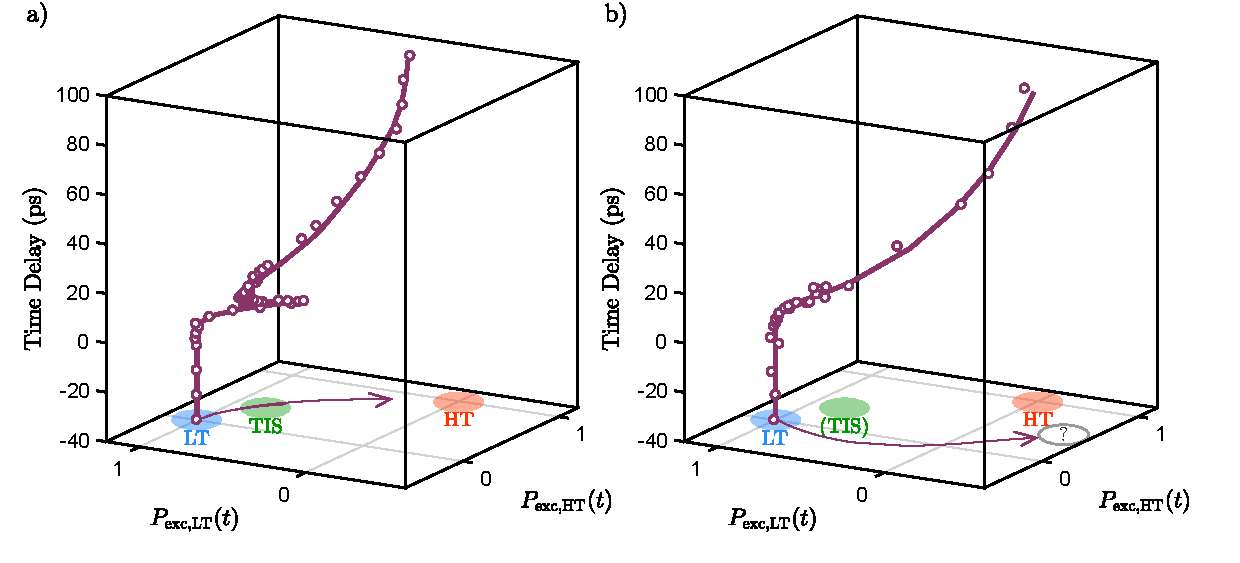
\includegraphics[width = \textwidth]{Figures/fig_EDOSb_Pearson.pdf}
  \caption[Time-dependent Pearson correlation of (EDO-TTF)\textsubscript{2}X
    (X = PF\textsubscript{6}, SbF\textsubscript{6}).]{
    Time-dependent Pearson correlation of the UED data of (EDO-TTF)\textsubscript{2}X,
    where X = (a) PF\textsubscript{6} and (b) SbF\textsubscript{6}.
    %
    For each time delay $t$, the correlation between the measured diffraction pattern of
    the photoexcited state and either equilibrium states is calculated
    ($P = 0$, no correlation; $P = 1$, perfect correlation).
    The thick line is a trajectory that is calculated
    using the fitted, interpolated UED intensities from global analysis;
    the thin line is the two-dimensional projection of the trajectory.
    Regions associated with the structures of identifiable states are labeled by colour.
  }
  \label{fig: EDOSb-Pearson}
\end{figure}
%
For $t < 0$~ps, both molecules are in the LT ground state at $(0, 1)$.
After $t = 0$~ps, they are photoexcited and the trajectories start to diverge from each other.
%
In Panel~(a), it can be seen that the structure of the (EDO-TTF)\textsubscript{2}PF\textsubscript{6} molecule
moves rapidly towards the HT state, overshoots, settles in the TIS at $(0.3, 0.9)$
for a few picoseconds, then finally relaxes to the final HT-like state.
%
On the other hand, in Panel~(b), the photoexcited structure of the X = SbF\textsubscript{6} derivative
evolves away from the structure of both the LT and HT states on a timescale of several tens of picoseconds,
bypassing the region of configuration space where its equivalent TIS structure would exist.
%
Indeed, the marked difference in shape of the two configuration trajectories
in Fig.~\ref{fig: EDOSb-Pearson} highlights the important role played by the counterion
in the PIPT of the (EDO-TTF)\textsubscript{2}X molecular system.

The earlier UED work on the X = PF\textsubscript{6} derivative
identified the three independent atomic motions that comprise the basis set for
fully describing the overall structural dynamics, one of these being the counterion motion
which is correlated with the formation of the TIS.
%
The present work recovers these modes in the form of the three principal components from the SVD analysis.
This suggests that the missing third mode in the X = SbF\textsubscript{6} UED data is
the counterion motion which would have steered its Pearson trajectory through the equivalent TIS region
in configuration space.
%
Thus, in a manner consistent with the proposed mechanism of Servol et~al~\cite{Servol2015},
the deactivation of the photoinduced IM~pathway in (EDO-TTF)\textsubscript{2}SbF\textsubscript{6} can be
explained by the conspicuous absence of this key mode.

Although the counterions are not directly involved in the photophysical process,
they play a crucial role in passively guided structural reorganization of the photoexcited cations.
This observation can be rationalized when the change in the local electric field due to
the photoinduced electron transfer between EDO-TTF molecules is considered.
%
In this view, the counterions move simply in response of the electrostatic reaction forces
and end up directing the lattice reorganization that destabilizes the charge-ordered state of the LT phase.
This motion is thus intimately coupled to the collective lattice response to photoexcitation
and the resulting change in material properties during PIPT.
In corollary, larger counterions would be too sterically encumbered to move accordingly,
preventing PIPT in isostructural derivatives of (EDO-TTF)\textsubscript{2}PF\textsubscript{6}
further down the chemical series. If the volume of the photoexcited LT unit cell could expand
on the ultrafast timescale and reduce steric hindrance, then this counterion effect may be less pronounced.

Fukazawa et~al also studied in their work~\cite{Fukazawa2013} the effect of counterion size
using time-resolved IR vibrational spectroscopy on the photoinduced phase transition of
another photoactive molecular system --- X[Pd(dmit)\textsubscript{2}]\textsubscript{2},
where X =  Cs and Et\textsubscript{2}Me\textsubscript{2}Sb%
\footnote{dmit = dimercaptoisotrithione or 1,3-dithiol-2-thione-4,5-dithiolate,
Et = C\textsubscript{2}H\textsubscript{5}, and Me = CH\textsubscript{3}.} ---
and observed that substitution for a larger counterion changes the order of the PIPT and
greatly delays the emergence of the final HT-like state
($\tau_\text{PIPT} = 0.1$~ps $\rightarrow 70$~ps).
%
The present UED results off the first direct structural evidence of the counterion effect
on lattice reorganization destabilizing the charge order of an insulator state and
the subsequent formation of a metallic state.
In particular, there are only a few types of atomic motions that dominate the structural transition,
as opposed to an equipartitioning to all possible degrees of freedom;
this phenomenon appears general and it is herein referred to as `dimensionality reduction'~\cite{Miller2016}.
The notion of key reaction modes has been discussed in the field of chemistry for some time;
they can now be observed directly using time-resolved structural probes like UED and
be used to explain how even a simple change in counterion can affect
the degree of lattice reorganization in charge-transfer processes and
be used to control macroscopic material properties.
%
Furthermore, this work has successfully demonstrated how SVD analysis belongs in the standard toolbox
for directly interpreting time-resolved diffraction data, without reliance on refinement models
that would map reciprocal-space features to real-space ones.

\subsection{Summary and Conclusions}

In this work, the structural dynamics of (EDO-TTF)\textsubscript{2}SbF\textsubscript{6} is
elucidated using a combination of SVD and Pearson analysis.
It is also the first comparative UED study of an isostructural family of molecules
with the goal of investigating the interplay between structural dynamics and molecular function
in close detail. The results show that the size of the counterion is a key factor for
determining the activity of the photoinduced IM~pathway and the dimensionality of
the associated atomic motions.
%
In the case of X = PF\textsubscript{6}, the structural dynamics is three-dimensional
in terms of generalized coordinates and one of three principal modes is
a counterion movement that leads to lattice relaxation and formation of the metallic state.
When X = SbF\textsubscript{6}, the dynamics becomes two-dimensional as the counterion is too large
and cannot avoid hindering the interactions between the EDO-TTF molecules;
this obstruction prevents full relaxation to the structural relationships
that enable the charge redistribution and spatial electron delocalization
necessary for the formation of a metallic band structure.
%
This conclusion is consistent with the mechanism proposed by others~\cite{Servol2015},
the interplay of cavity size and counterion size~\cite{Kistenmacher1984},
and the general sensitivity of (EDO-TTF)\textsubscript{2}X~\cite{Nakano2008, Nakano2009, NakanoX, Ishikawa2014}
and Bechgaard-Fabre salts~\cite{Kohler2011, Dressel2012, Pouget2018} to chemical and
isotope substitution.

In particular, the present work is not based on structural refinement models;
instead, it is understood using SVD in reciprocal space, an approach that has been
well-established for spectroscopic techniques involving overlapped spectra components.
Here, SVD is used as an unbiased method to analyze time-resolved diffraction data and
project out the dominant atomic motions involved in the structural dynamics.
%
There are clearly only a few key modes, greatly reducing the dimensionality of
the problem of chemistry:
the convolution of all nuclear motions possible in a reaction mechanism
to a single putative coordinate for the purpose of controlling molecular processes.
%
Indeed, these findings illustrate the great promise that the techniques used herein
bears for further application to other diffraction experiments.


% Dressel2012:
% charge disproportionation/imbalance (reflectivity) <-> vibrational modes (IR, Raman)
% larger anion -> larger intrastack distance ->? more pronounced intersite Coulomb repulsion
% anion-sulfur distance vs. charge ordering
% lattice vib. coupling modulates transfer integral, intramolecular vib. coupling modulates on-site energy
% HOMO of molecule shows charge mainly located on sulfur atoms and C=C bonds
% motion of anions slows down with low T, lock in place inside cavity (anion rotational disorder lifted) -> anion ordering <- anion-F-S long-range interaction
% charge disproportionation increases from PF6 to SbF6

% Role of cavity and anion size in TMTSF salts (1984):
% Kistenmacher, T.J. Cavity sice versus anion size in (TMTSF)2X salts - possible implications for the uniqueness of (TMTSF)2ClO4. Solid State Commun. 1984, 50, 729–733.
% Kistenmacher, T. Anion-donor coupling in (TMTSF)2X salts—Symmetry considerations. Solid State Commun. 1984, 51, 931–934.

% Deuteration modulates the electron-molecular-vibration (e-mv) coupling and
% increases the transition temperature by $3.5$~K
% Substituent effect (CLEDO-TTF and MeEDO-TTF)

  
\chapter{Photocyclization Dynamics of Diarylethene}
\label{ch: UED-DAE}

The focus of this chapter is a study that uses UED to probe the atomic motions
that take place during the `photocyclization' or
photoinduced ring-closing reaction of the molecule
1,2-bis(2,4-dimethyl-5-phenyl-3-thienyl)perfluorocyclopentene,
herein abbreviated to PFC.
%
I will give an overview on the properties and photophysics of the family of molecules
known as `diarylethene,' to which PFC belongs.
%
Then, I will describe the experimental methods involved and
finally discuss the results from the measurements. Large portions of this chapter
is based on the work described in the article ``Ring-Closing Reaction in Diarylethene
Captured by Femtosecond Electron Crystallography'' previously published in
the Journal of Physical Chemistry~B~\cite{Jean-Ruel2013}.

\section{Overview of Diarylethenes}
\label{sec: UED-DAE-Intro}

A diarylethene is a pair of double-bonded carbon atoms with an aryl%
\footnote{An aryl is any molecular substituent derived from an aromatic ring,
e.g.~phenyl (C\textsubscript{6}H\textsubscript{5}--) is
the aryl of benzene (C\textsubscript{6}H\textsubscript{6}).} group attached to each end;
%
Its chemical derivatives form a distinct family of molecules that exhibit `photochromism' or
light-induced reversible colour change by chemically transforming between isomers
with different absorption spectra.
%
As seen in Fig.~\ref{fig: DAE-overview}, they go from colourless to coloured and
the absorption of the photogenerated state can be tuned across the visible spectrum
with appropriate modification of the base molecular structure.
%
In particular, DAEs are `P-type' photochromes;
their coloured forms are thermodynamically stable and can only be converted back photochemically.
Others photochromes, like azobenzenes and spiropyrans, have thermally driven back-reactions
and are thus known as `T-type.'
%
This means that the photochromic state of P-type DAEs is non-volatile and
can be addressed and changed using light only, properties that make such molecules
prime candidates for use in optoelectronics, such as optical memory devices and photoswitches,
and in optomechanics, as light-driven actuators and molecular machines~\cite{Irie2000, Irie2014}.

\begin{figure}[t!]
  \centering
  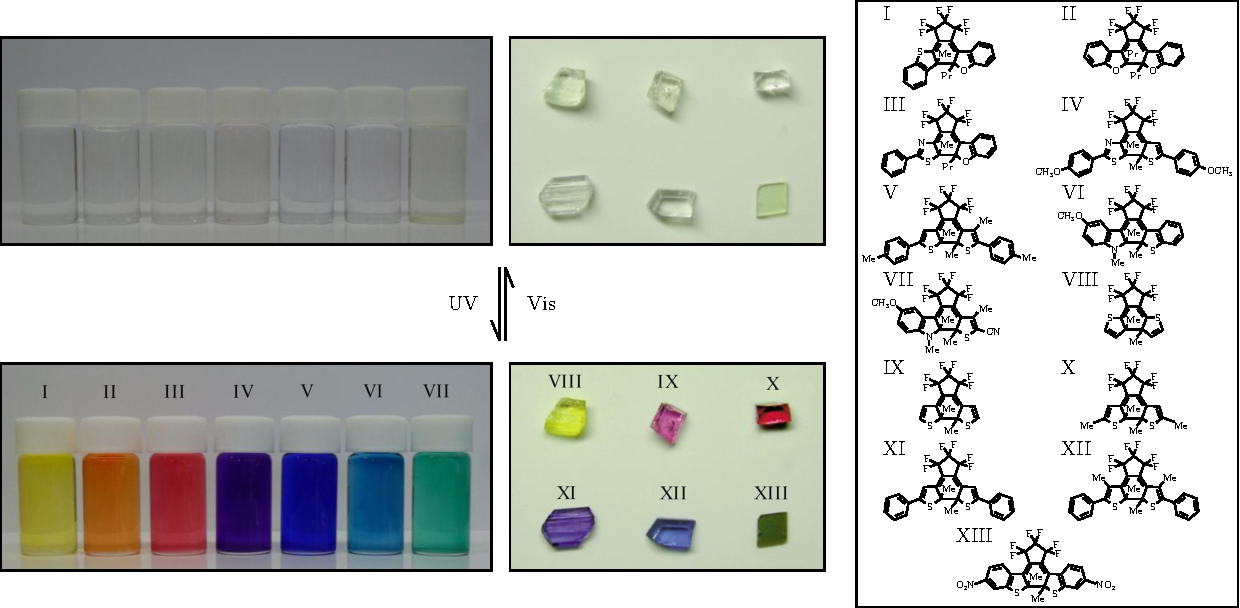
\includegraphics[width = \textwidth]{Figures/fig_DAE_overview.pdf}
  \caption[Photochromism of diarylethene derivatives.]{
    Photochromism of diarylethene derivatives in toluene~(left) and
    in single crystal~(centre) under $266$-nm light;
    their molecular structures are shown on the right.
    Adapted with permission from Ref.~\cite{Irie2014}.
  }
  \label{fig: DAE-overview}
\end{figure}

A prototypical diarylethene is 1,2-diphenylethene or stilbene~(\textbf{1});
As shown in Fig.~\ref{fig: DAE-stilbene}, its colourless \textit{cis}%
\footnote{The prefixes \textit{cis} and \textit{trans} denote the side on which
a pair of functional groups is relative to a carbon chain:
\textit{cis} = same side; \textit{trans} = opposite sides.}
or open-ring~(OR) form can reversibly photoisomerize under UV radiation to
the \textit{trans} form~(\textbf{2})
or undergo `photocyclization'~(ring-closing) and become yellow 4a,4b-dihydrophenanthrene~(\textbf{3}).
In the absence of oxygen, this coloured closed-ring~(CR) conformer
quickly reverts back to \textbf{1} in the dark via `cycloreversion'~(ring-opening);
otherwise, it oxidizes irreversibly to phenanthrene~\cite{Bao2011}.
%
\begin{figure}[ht!]
  \centering
  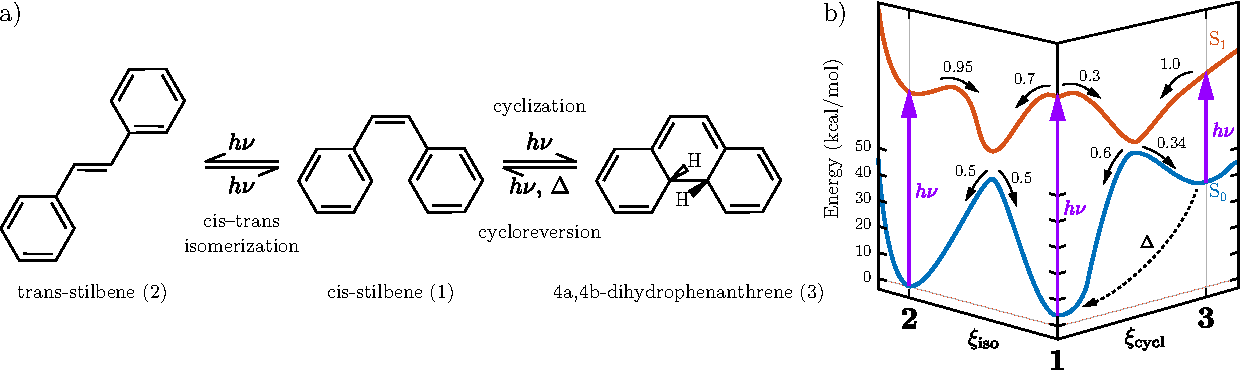
\includegraphics[width = \textwidth]{Figures/fig_DAE_stilbene.pdf}
  \caption[Photochemical reactions of \textit{cis}-stilbene.]{
    Photochemical reactions of \textit{cis}-stilbene.
    (a) Under UV exposure, \textit{cis}--\textit{trans} isomerization,
    cyclization, and cycloreversion can occur.
    (b) Schematic of the potential energy surfaces of the S$_1$ photochemical processes
    of stilbene along the two reaction coordinates;
    approximate quantum yields and branching ratios are indicated.
    Adapted with permission from Ref.~\cite{Repinec1991}.
  }
  \label{fig: DAE-stilbene}
\end{figure}

As noted in Ref.~\cite{Irie2014},
a DAE molecule optimized for the practical applications laid out earlier ought to satisfy
the following requirements:
%
\begin{enumerate}
  \item thermal stability of both colourless and coloured isomers;
  \item resistance to fatigue over multiple photocycles;
  \item high quantum yield;
  \item ultrafast response;
  \item activity in solid state;
  \item sensitivity in the near-IR region (650--830~nm).
\end{enumerate}
%
Clearly, \textit{cis}-stilbene is inadequate and a great number of derivatives
have been chemically synthesized to remediate its lackluster photochromic properties~\cite{Szaloki2013}.
One substitution pathway is as follows.
To prevent thermal cycloreversion of \textbf{1}, the phenyl groups are replaced by
thiophene rings which reduce the aromaticity, and thus the ground state energy,
of the coloured CR isomer~\cite{Irie1988, Irie1989}.
%
To stabilize the ring-closed isomer against oxidation and optical fatigue,
methyl groups are substituted at both \textit{ortho}-positions
of the thiophene--ethene bond~\cite{Irie1999, Higashiguchi2000};
%
To increase the quantum yield of the photochromic cyclization,
the \textit{cis}--\textit{trans} photoisomerization is blocked
by replacing the ethene moiety with a cyclopentene ring;
fluorination of this ring speeds up the ring closure (from $4.2$ to $0.9$~ps)~\cite{Hania2005}.
%
Substitution of a phenyl ring onto each thiophene ring increases
the peak absorption coefficient~$\epsilon$ of the CR isomer
(from $5.0 \times 10^3$ to $1.1 \times 10^4$~M$^{-1}$~cm$^{-1}$)
and shifts its absorption maximum a bit closer to the near-IR (from $534$ to $560$~nm%
\footnote{In benzene.})~\cite{Irie2014}.
The result is a diarylethene derivative called
1,2-bis(2,4-dimethyl-5-phenyl-3-thienyl) perfluorocyclopentene~(PFC)
and its molecular structure is shown in Fig.~\ref{fig: DAE-PFC}a.

\begin{figure}[t!]
  \centering
  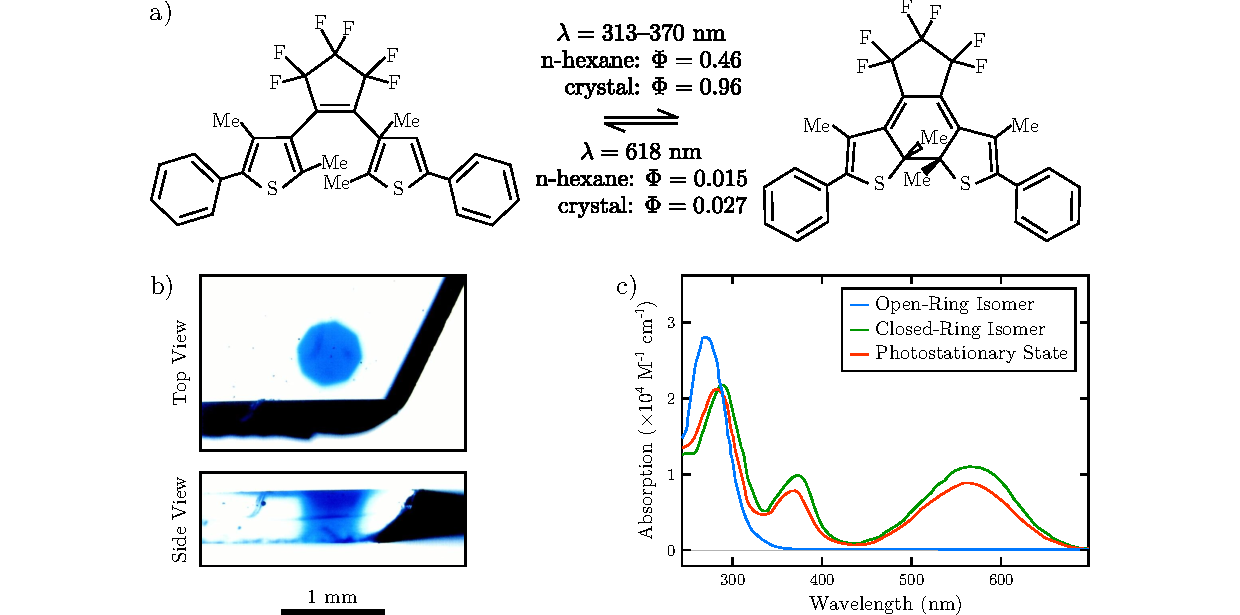
\includegraphics[width = \textwidth]{Figures/fig_DAE_PFC.pdf}
  \caption[Overview of 1,2-bis(2,4-dimethyl-5-phenyl-3-thienyl)perfluorocyclopentene.]{
    Overview of photochromism in PFC:
    (a) molecular structure,
    (b) photochromism in single-crystal (top and side view, circular spot under 366-nm light), and
    (c) absorption spectrum in n-hexane of the open-ring and closed-ring conformations;
    The values for the quantum yield $\Phi$ of the ring-closing/opening reactions
    in n-hexane and in single-crystal in Panel~(a) are taken from
    Refs.~\cite{Irie1995, Shibata2002} respectively.
    Panels~(b) and (c) are adapted with permission
    from Refs.~\cite{Irie2001} and~\cite{Irie1995} respectively.
  }
  \label{fig: DAE-PFC}
\end{figure}

PFC is a DAE molecule that has been often studied
since it is first reported by Irie et al~\cite{Irie1995}.
%
As seen in Fig.~\ref{fig: DAE-PFC}c,
the OR isomer of this molecular system is transparent to visible light,
absorbing strongly in the UV part of the spectrum%
\footnote{Absorption of PFC in n-hexane: $\lambda_\mathrm{max} = 268$~nm (OR) and $562$~nm (CR),
$\epsilon = 2.84 \times 10^4$~M$^{-1}$~cm$^{-1}$ (OR)
and $1.09 \times 10^4$~M$^{-1}$~cm$^{-1}$ (CR)~\cite{Irie1995}.}
to drive photocyclization to the CR conformation which appears blue (Fig.~\ref{fig: DAE-PFC}b).
%
In single crystal, this change in molecular structure is sufficiently large
to create regular $1$-nm tall steps and ridges on the material surface
that disappear upon cycloreversion~\cite{Irie2001}.
%
Furthermore, the quantum yield of the ring-closing reaction in this state
is more than double that in the solution phase
since all the thiophene side-groups of the OR isomers are locked in an anti-parallel conformation
wherein the reactive carbon atoms are in close proximity~\cite{Shibata2002};
in solution, the substituents are free to rotate and $52$~\% of them are aligned in parallel,
causing the molecule to be nonreactive to photocyclization~\cite{Irie1995, Pontecorvo2014}.

A large number of works has studied the electronic reaction dynamics of
photo-cyclization and -cycloreversion of DAE derivatives in the solution phase
using time-resolved spectroscopic techniques;
indeed, the processes were found to be ultrafast,
having taken place within a few picoseconds~\cite{Irie2014}.
%
More relevant to UED are some studies which were made on PFC and its close relatives
in the crystalline phase~\cite{Miyasaka1997, Ishibashi2007, Tani2008, Jean-Ruel2011}.
%
In particular, Jean~Ruel et al~\cite{Jean-Ruel2011} followed the excited-state dynamics
of the OR$\rightarrow$CR process on subpicosecond time scale
by pumping ca.~$100$-$\unslant\mu$m thick crystals with $100$~fs pulses at $343$~nm
and measuring the transient absorption spectra with a IRF time $\tau_\mathrm{IRF}$ of $(130 \pm 20)$~fs;
complete cycloreversion in between each pump-probe event is ensured
by illuminating the sample position with a $500$-ms pulse at $633$-nm from a helium-neon laser.

The first observation is that PFC can undergo $3 \times 10^4$ photochromic cycle
and still show no sign of optical fatigue.
%
The second is that the ring-closing reaction proceeds in three characteristic steps.
As seen on the left side of Fig.~\ref{fig: DAE-PFC-TA}a, the UV pump pulse generates an excited state
with an initially broad absorption spectrum that narrows and redshifts over $\tau_1 \sim 200$~fs;
the feature at $490$~nm then decays over $\tau_2 = 5.3$~ps
while another at $635$~nm matching the CR absorption peak appears over $\tau_3 = 7.3$~ps.
%
This reaction dynamics can be explained using the ground- and excited-state
potential energy surface topology calculated for a model DAE similar to PFC~\cite{Boggio2003}:
the initial state is a hot OR molecule in the geometry of the S$_0$ OR minimum;
this excited state relaxes to the OR minimum on the S$_1$ surface over $\tau_1$
and then evolves along an orthogonal reaction coordinate to a conical intersection
where it radiationlessly undergoes ring closure in $\tau_2$ and vibrationally cools
to the $S_0$ CR minimum over $\tau_3$.

\begin{figure}[t!]
  \centering
  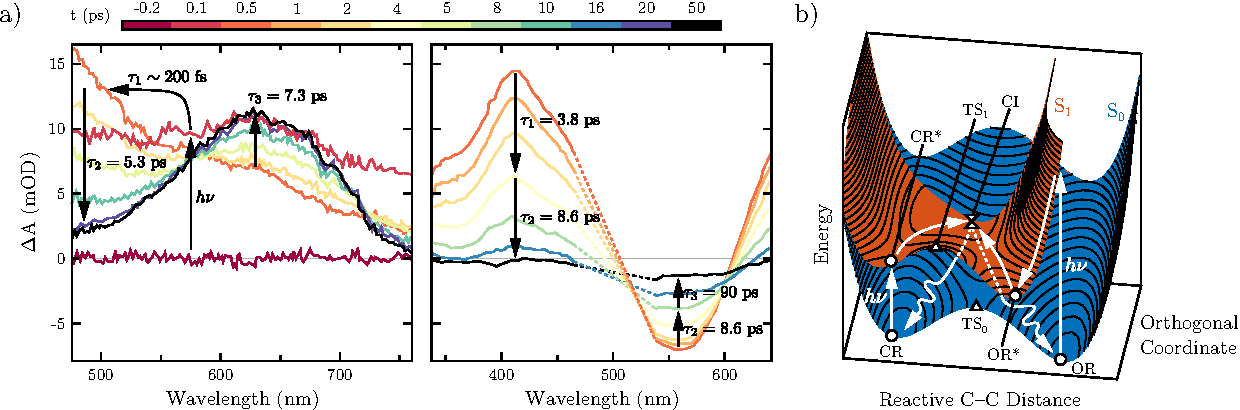
\includegraphics[width = \textwidth]{Figures/fig_DAE_PFC_TA.pdf}
  \caption[Ultrafast reaction dynamics of photochromism.]{
    Ultrafast reaction dynamics of photochromism in PFC:
    (a) transient absorption measurements of the ring-closing (left)
    and ring-opening (right) reactions;
    (b) schematic representation of the two corresponding reaction pathways
    on the S$_0$, S$_1$ potential energy surfaces of a model DAE similar to PFC.
    Panel~(a) is adapted with permission from Refs.~\cite{Jean-Ruel2011}~(left) and~\cite{Ward2012}~(right),
    and Panel~(b), from Ref.~\cite{Boggio2003}.
  }
  \label{fig: DAE-PFC-TA}
\end{figure}

Similarly, the dynamics of the cycloreversion of PFC (in cyclohexane) has been observed
by Ward et al~\cite{Ward2012}.
The right side of Fig.~\ref{fig: DAE-PFC-TA}a shows their femtosecond TA spectra where
there is excited state absorption (ESA) and ground state bleach (GSB)
centered at $410$ and $560$~nm, respectively.
%
In terms of the energy schematic in Panel~(b), the ESA which decays over $\tau_1 = 3.8$~ps
is assigned to dynamics on the S$_1$ surface as the CR molecule evolves to the same conical intersection.
the spectral component with $\tau_2 = 8.6$~ps is the actual ring-opening reaction as the excited state
decays onto the S$_0$ surface;
the GSB disappears over $\tau_3 = 90$~ps as
almost all the photoexcited molecules cool and return to the S$_0$ CR geometry
due to the low quantum yield of photocycloreversion process in PFC.

Since spectroscopic techniques are only sensitive to structural dynamics
through the associated changes in electronic energy levels,
the focus of the UED work presented herein is to directly observe the atomic motions involved in
the photocyclization of single-crystal PFC and
provide a complementary description of the reaction dynamics.

\section{Methods}
\label{sec: UED-DAE-methods}

\begin{figure}[ht!]
  \centering
  \includegraphics[width = \textwidth]{Figures/fig_DAE_PFC_photo.pdf}
  \caption[Sample preparation and qualification under the pump-probe-HeNe scheme.]{
    (a) Photo of a PFC crystal ready for ultramicrotomy.
    (b) Normalized intensity of the $(5 1 \overline{6})$ diffraction spot
    before (blue) and after (ref) the pump laser pulse for the first 12
    photocyclization--photocycloreversion cycles, showing the reversible transformation
    of single-crystal PFC between its two conformations under the pump-probe-HeNe scheme.
    Panel~(b) is adapted with permission from Ref.~\cite{Jean-Ruel2013}.
  }
  \label{fig: DAE-PFC-Photo}
\end{figure}

% Sample preparation
PFC can be readily synthesized from base reactants using the procedure of Irie et al~\cite{Irie1995}.
Here, it is purchased in powder form from a commercial supplier (Tokyo Chemical Industrial Co.)
and dissolved in hexane at $5$~g/L.
Colourless crystals are grown in the dark by slow solvent evaporation from a flat bottom beaker
and the largest ones (ca.~$500$~$\unslant\mu$m $\times$ 500~$\unslant\mu$m $\times$ 100~$\unslant\mu$m)
are selected for sample preparation.

As in the case of (EDO-TTF)\textsubscript{2}X in Sec.~\ref{sec: UED-EDOPF6}, the chosen crystal
is glued to epoxy resin (Fig.~\ref{fig: DAE-PFC-Photo}a) and cleaved into slices $100$--$150$~nm thick by ultramicrotomy.
These thin single-crystal slices are then mounted on TEM copper mesh grids
with lacy formvar support membranes. To obtain samples with different crystal orientations,
the crystals are cleaved along different planes.

% UED and laser conditions
The UED measurements are conducted in the same experimental setup as in Sec.~\ref{sec: UED-EDOPF6}
with some PFC-specific modifications.
%
To excite the PFC sample near the optimal wavelength for photocyclization,
the pump beam is made by splitting the $267$-nm output of the THG setup before it is
used to generate the probe electron pulses; the fluence and spot size are set to $0.35$~mJ/cm$^2$
and $600$~$\unslant\mu$m at the sample position and the pulses are stretched to ca.~$300$~fs in an effort
to minimize the laser peak power and thus avoid artifacts due to multiphoton ionization.
%
The probe electron pulses are $70$-fC (ca.~$4.4 \times 10^5$~e$^{-}$) bunches
with a spot size of $400$~$\unslant\mu$m FWHM that is centered on the pump spot.
%
Since the closed-ring state of PFC is stable, simply allowing any time between pump-probe events
for thermal relaxation is not feasible to ensure an open-ring sample volume before each measurement.
Instead, a third laser pulse --- $633$~nm, $2$~mW, $100$~ms --- from a helium-neon (HeNe) laser illuminates
the sample $2$~ms after the pump pulse and triggers complete cycloreversion over
a spot size of $700$~$\unslant\mu$m.
%
Thus, the repetition rate of the measurements is necessarily reduced to a paltry $0.1$~Hz,
much slower than that of usual UED experiments.
%
Fig.~\ref{fig: DAE-PFC-Photo}b shows the normalized intensity of a diffraction spot sensitive to
the ring-closing reaction before (blue) and after (red) the pump pulse
for the first dozen (and 400 in the inset) pump-probe-HeNe cycles;
the steadiness of the signal confirms the reversibility of the photoinduced structural dynamics in PFC
under this pump--probe--HeNe scheme.

\begin{figure}[ht!]
  \centering
  \includegraphics[width = \textwidth]{Figures/fig_DAE_PFC_structure.pdf}
  \caption[Crystal structure of PFC and orientation determination.]{
    ORTEP~representations of the molecular structure of PFC
    in its (a) open-ring and (b) closed-ring conformation,
    and (c) crystal packing in the $(010)$~plane.
    Scatter plots of the (d) experimentally measured and (e) simulated
    diffraction data for a sample with orientation $[ 0.45, 0.19, 0.87]$ are shown
    and (f) overlain for comparison;
    the size of the markers scales with the intensity of the diffraction spots.
    Panels~(a)--(c) and (d)--(f) are adapted with permission from Refs.~\cite{Irie2001}
    and~\cite{Jean-Ruel2013} respectively.
  }
  \label{fig: DAE-PFC-structure}
\end{figure}

To index and interpret the measured UED signals,
the crystal orientation of the samples relative to the incident electron direction needs to be determined.
Here, a simulation-based refinement scheme
--- described in more detail in Sec.~\ref{sec: UED-data-analysis-1} --- is used.
%
The crystal structures of the OR and CR conformers of PFC are shown
in the top three panels of Fig.~\ref{fig: DAE-PFC-structure} from Irie et al~\cite{Irie2001}.
Starting from this information, the simulated intensity and position of diffraction spots
are calculated and matched to the observed values
by maximizing the goodness-of-fit which is the Pearson correlation coefficient $P_\mathrm{sim, exp}$
as in Fig.~\ref{fig: UED-orientation}a.

In the bottom three panels of Fig.~\ref{fig: DAE-PFC-structure},
the experimentally measured and simulated diffraction spots
are compared to show the effectiveness of this refinement scheme.
%
The result is a crystal orientation~$k_\mathrm{inc} = [ u_1, u_2, u_3]$ for each measured PFC sample
with R-factors between $0.23$ and $0.34$.
%
Using these values, Eq.~\eqref{eq: nexc}, and the intensity of 22 reliable diffraction spots,
the excitation fraction $\eta_\mathrm{exc}$ is estimated to be $2.9$~\%,
as expected from the low laser fluence of the pump beam.

To make the molecular movie of PFC, a model of the structural dynamics is needed.
Previously, as in Eq.~\eqref{eq: linear-model},
the atoms are constrained to move linearly between their known ground- and excited-state
positions.
In this case, it is found by inspection that the OR~conformation
can be transformed to the CR~one using only four motions: three rotations
and a rotation plus torsion (see Fig.~\ref{fig: DAE-PFC-model})
%
Then, the measured diffraction intensities can be refined against
those evaluated from this four-parameter model to obtain
a molecular structure of PFC at each probed time point
using the methods described in Sec.~\ref{sec: UED-data-analysis-3}.

\begin{figure}[t!]
  \centering
  \includegraphics[width = \textwidth]{Figures/fig_DAE_PFC_model.pdf}
  \caption[Four-motion structure model of PFC ring closure.]{
    Front and top skeleton view of the four motions which transform the PFC molecule
    from its OR ($\xi = 0$) to CR ($\xi = 1$) conformation in two steps of $\Delta \xi = 0.5$.
    Adapted with permission from Ref.~\cite{Jean-Ruel2013}.
  }
  \label{fig: DAE-PFC-model}
\end{figure}

% Computational methods
In support of the UED molecular movie, an ab initio model of the ring closing reaction
in the single-crystal state is implemented in the subtractive QM/QM paradigm,
a hybrid computational scheme that offers reasonable accuracy in large molecular systems.
%
Briefly, the set of all atoms $\mathbb{S}$ is partitioned into an inner subset $\mathbb{I}$
and an outer subset $\mathbb{O}$ consisting respectively of the few atoms of the reaction centre
and the many others that are mostly spectators;
different levels of quantum mechanical approximation can then be applied,
with the highest and computationally most expensive level one $\mathbb{I}$ and the lowest on $\mathbb{O}$,
and the total QM/QM energy of the system is thus given by
%
\begin{equation}
  \begin{aligned}
    E_\mathrm{QM/QM}(\mathbb{S}) & = E_\mathrm{LQM}(\mathbb{S})
      + E_\mathrm{HQM}(\mathbb{I} \cup \mathbb{L}) - E_\mathrm{LQM}(\mathbb{I} \cup \mathbb{L})
  \end{aligned}
  \label{eqn: QMQM}
\end{equation}
%
where $\mathrm{HQM}$ and $\mathrm{LQM}$ are applicable high- and low-level QM methods and
$\mathbb{L}$ is the set of `linkers,' extra hydrogen atoms added to cap any dangling covalent bond
in the boundary between $\mathbb{I}$ and $\mathbb{O}$~\cite{Senn2006, Vreven2006, Kochman2013}.
%
Here, the UED sample is modeled as a bulk lattice where only one of the four PFC molecules
in the unit cell is photoreactive.
In the QM/QM scheme of this work, $\mathbb{S}$ is the set of all the atoms in a single unit cell
and $\mathbb{I}$ consists of the 1,2-bis(2,4-dimethyl-3-thienyl)pentene moiety
of one of the PFC molecules (see Fig.~\ref{fig: DAE-PFC-QMQMmodel}).
%
$E_\mathrm{LQM}(\mathbb{S})$ is calculated on the level of density functional theory~(DFT)
using a plane wave basis set%
\footnote{The plane wave cut-off is set at 400~eV;
the electronic Brillouin zone is sampled at the $(0 \frac{1}{4} 0)$ $k$-point only;
the default ultrasoft pseudopotentials in \textsc{CASTEP} are used;
energies and forces are corrected for dispersion interactions as in Ref.~\cite{Grimme2006}.}
and the Perdew-Burke-Ernzerhof~(PBE) exchange-correlation functional
as implemented in \textsc{CASTEP}~5.0;
%
$E_\mathrm{LQM}(\mathbb{I} \cup \mathbb{L})$ is similarly evaluated but
using the localized Gaussian-type 3-21G(d) orbital basis.
%
Finally, $E_\mathrm{HQM}(\mathbb{I} \cup \mathbb{L})$ is calculated at the level of
complete-active-space self-consistent field~(CASSCF) theory%
\footnote{An active space consisting of 10 canonical $\pi$- and $\pi^*$-type orbitals
is used.} as implemented in \textsc{Gaussian}~09 using the localized 3-21G basis set.

\begin{figure}[ht!]
  \centering
  \includegraphics[width = \textwidth]{Figures/fig_DAE_PFC_QMQMmodel.pdf}
  \caption[Partitioning of PFC unit for QM/QM~calculations.]{
    Partitioning of the atoms of the PFC~unit cell into two subsets, $\mathbb{I}$ and $\mathbb{O}$,
    for hybrid QM/QM calculations.
    Adapted with permission from Ref.~\cite{Irie2001, Jean-Ruel2013}.
  }
  \label{fig: DAE-PFC-QMQMmodel}
\end{figure}


\section{Experimental Results and Discussion}
\label{sec: UED-DAE-results}

% UED patterns
In Fig.~\ref{fig: DAE-PFC-UED}, time-resolved electron diffraction data
of single-crystal PFC are shown in three different crystal orientations.
From Panels~(a)--(c), the patterns are well ordered to high diffraction orders and
many spots can be clearly observed.
%
To evaluate the sensitivity of the UED setup to the ring-closing reaction,
pump-probe UED images are taken at a time delay corresponding to $t_\infty$
and compared to simulated ones, calculated using Eq.~\eqref{eq: diff-int}
and the known XRD structures of the open- and closed-ring molecules from Ref.~\cite{Irie2001}.
%
These $t_\infty$ difference images are shown in Panels~(d)--(f) and
it can be observed that a large number of diffraction spots exhibit
significant and divergent changes in intensity, indicative of
atomic displacement within the unit cell.
%
The close match between these changes with the simulated ones in Panels~(g)--(i)
demonstrates that UED can probe the relevant structural dynamics of PFC.
%
\begin{figure}[ht!]
  \centering
  \includegraphics[width = \textwidth]{Figures/fig_DAE_PFC_UED_.pdf}
  \caption[Time-resolved electron diffraction patterns of PFC.]{
    Time-resolved electron diffraction data of PFC samples
    with different crystal orientations:
    (a) $[ 0.45, 0.19, 0.87]$; (b) $[ -0.77, 0.17, -0.62]$; (c) $[ 0.87, -0.02, 0.49]$.
    Row-wise, Panels~(a)--(c) show the static UED patterns;
    (d)--(f), the pump-probe difference intensities at $t_\infty$;
    (g)--(i), the simulated difference intensities assuming an excitation fraction of $2.9$~\%
    and using the known XRD structures of the open- and closed-ring molecules.
    Adapted with permission from Ref.~\cite{Jean-Ruel2013}.
  }
  \label{fig: DAE-PFC-UED}
\end{figure}

% Time traces
Fig.~\ref{fig: DAE-PFC-UEDtraces} shows the temporal evolution in intensity of four select
diffraction spots, chosen because they are representative of all the changes observed
in the UED dataset of PFC.
%
\begin{figure}[ht!]
  \centering
  \includegraphics[width = \textwidth]{Figures/fig_DAE_PFC_UEDtraces.pdf}
  \caption[Select UED time traces of single-crystal PFC.]{
    Select UED time traces of single-crystal PFC showcasing
    the different type of time-dependent intensity changes
    in the measured diffraction patterns:
    (a) $(5 1 \overline{6})$;
    (b) $(5 \overline{1} \overline{2})$;
    (c) $(2 0 \overline{2})$;
    (d) $(2 0 \overline{4})$.
    Adapted with permission from Ref.~\cite{Jean-Ruel2013}.
  }
  \label{fig: DAE-PFC-UEDtraces}
\end{figure}

The UED signals in Panels~(a) and (b) are typical to many diffraction spots:
an ultrafast change that develops over a few picoseconds and stays until $t_\infty$.
Since the $t_\infty$ intensity difference corresponds to the closed-ring structure,
they are directly attributed to the structural dynamics associated with
the ring-closing reaction.
Furthermore, monoexponential fit of these two time traces yield
two different time constants: $\tau_1 = (3 \pm 1)$~ps and $\tau_2 = (5 \pm 3)$~ps respectively.
These values agrees with the results of previously reported TA measurements~\cite{Jean-Ruel2011},
where a time constant of $5.3$~ps was found for the orthogonal evolution of
excited state on the S$_2$ potential energy surface from the excited open-ring intermediate (OR$^*$)
to the closed-ring (OR) structure (see Fig.~\ref{fig: DAE-PFC-TA}b).

Fig.~\ref{fig: DAE-PFC-UEDtraces}c shows another type of UED signal that is observed
for a number of diffraction spots; it consists of a very slow $80$-ps change of large amplitude
that vanishes between $t = +100$~ps and $t_\infty$.
This transient behaviour does not reflect the thermally irreversible structural change
associated with photocyclization.
Instead, it is indicative of strain waves generated by the mechanical stress of
some PFC molecules contracting volumetrically as they are photoexcited and undergo ring closure.
From Ref.~\cite{Irie2001}, a PFC molecule flattens and shrinks during the OR$\rightarrow$CR transformation,
with its width%
\footnote{As measured by the distance between the methyl groups ortho to the reactive carbon atoms.}
decreasing by ca.~$20$~\%.
Similar strain signals are observed in the late-time UED data of (EDO-TTF)\textsubscript{2}X
(see the left side of Fig.~\ref{fig: EDO-TRresults}b).
Conveniently, since these intensity changes are few, easily identified as signal modulations,
and well separated in time, they do not prevent the monitoring of the photocyclization process by UED.
Indeed, the Pearson correlation coefficient between
the experimental $\Delta I/I_\mathrm{off}$ averaged over $t = +10$ and $+50$~ps and
the simulated ones is $0.92$ when only strain-free diffraction spots are considered.

Finally, Fig.~\ref{fig: DAE-PFC-UEDtraces}d presents a UED signal
that clearly appears within a picosecond and is followed by a slow transient feature
caused by the crystal strain.
The observation of this ultrafast signal is a key result of the present work
since its time scale is consistent with that of the evolution on the S$_2$ potential energy surface
prior to ring closure ($\tau_1$ in the left side of Fig.~\ref{fig: DAE-PFC-TA}a),
from the initial open-ring Franck-Condon state to the open-ring intermediate state
(OR$^*$ in Fig.~\ref{fig: DAE-PFC-TA}b).
Thus, the existence of an intermediate PFC structure, forming in these times and
clearly distinct from the closed-ring one, is confirmed.

% Model results
% Figure: 0 ps, +10 ps structures, histogram
To reconstruct the real-space molecular movie of PFC as it undergoes photocyclization,
the four-motion model set up in Fig.~\ref{fig: DAE-PFC-model} is employed,
with a focus on the structure of the intermediate state that forms soon after photoexcitation.
%
As prescribed in Sec.~\ref{sec: UED-data-analysis-3},
the four components of the reaction coordinate $\boldsymbol{\xi} = (\xi_1, \xi_2, \xi_3, \xi_4)$
are independently varied from $-0.5$ to $1.5$ to generate a large pool of candidates,
where the coordinates $\boldsymbol{\xi} = (0, 0, 0, 0)$ and $(1, 1, 1, 1)$ represent
the ground OR and CR structures respectively (see Panels~(a) and (b) of Fig.~\ref{fig: DAE-PFC-results}).
%
The structure factors of each generated structure, $F_\mathrm{sim}(\boldsymbol{\xi}), \boldsymbol{q}_j$,
is then simulated under the kinematical approximation and compared to the experimentally measured one,
$F_\mathrm{on, exp}(t, \boldsymbol{q}_j)$, using the Pearson correlation coefficient,
$P_\mathrm{sim, exp}(\boldsymbol{\xi}, t)$, as the GoF.
%
Given the limited~SNR of the experimental data, the analysis uses only
the $18$~brightest strain-free diffraction spots and the optimal reaction coordinate
for a given time point, $\boldsymbol{\xi}_\mathrm{opt}(t)$,
is defined as the average of the subset of coordinates
which generates the top $1$~\% best-matching structures.

\begin{figure}[t!]
  \centering
  \includegraphics[width = \textwidth]{Figures/fig_DAE_PFC_results.pdf}
  \caption[Structural dynamics of PFC in the four-motion model.]{
    Structural dynamics of PFC in the four-motion model:
    comparing (a) the $(1, 1, 1, 1)$ structure with those of
    the ground conformations after geometry optimization;
    (b) the lower and upper bounds of the searched coordinate space;
    (c) the optimal structures that best fit the pump-off ($t \leq 0$~ps)
    and late-time ($t \geq 10$~ps) data.
    Adapted with permission from Ref.~\cite{Jean-Ruel2013}.
  }
  \label{fig: DAE-PFC-results}
\end{figure}

In Fig.~\ref{fig: DAE-PFC-results}c, the model PFC structures
generated by $\boldsymbol{\xi}$ optimized for the pump-off ($t \leq 0$~ps)
and late-time ($t \geq 10$~ps) diffraction data are shown.
By inspection, both are consistent with the known structures of
the ground OR and CR conformers.
%
The positions of the two methyl groups ortho to the reactive carbon atoms
have not converged to their expected CR values, likely due to
weak contribution to the diffraction intensities in the crystal orientations sampled here.

A key point of interest in the photocyclization process of PFC is
the structural dynamics that occur at early time,
before the actual ring closure itself.
%
Here, inspection of $\boldsymbol{\xi}_\mathrm{opt}(t)$ for $t$ from $+0.5$ to $+3.0$~ps
(see Fig.~\ref{fig: DAE-PFC-results-QMQM}a) suggests that
the dominant atomic motion resolved in the UED data is
a full rotation of the thiophene moieties combined with
a partial rotation of the perfluorocyclopentene ring.
%
This conformation is distinct from those of the ground states (OR and CR);
it is tentatively assigned to the open-ring excited state (OR$^*$ in Fig.~\ref{fig: DAE-PFC-TA}b)
proposed by the theoretical work of Boggio-Pasqua et~al
for a free PFC molecule~\cite{Boggio2003}.

To validate the assignment of the early-time UED intermediate to
the OR$^*$ state, ab initio calculations are performed,
extending the Boggio-Pasqua work~\cite{Boggio2003} to the single-crystal phase.
%
As described in Sec.~\ref{sec: UED-DAE-methods} and shown in Fig.~\ref{fig: DAE-PFC-QMQMmodel},
the reaction centre of the photoexcited molecule is described at the CASSCF level of theory
while the rest of the molecule and unit cell is treated at the lower DFT level.
The result is a reaction intermediate embedded in a crystal lattice of ground-state molecules,
all fully optimized.
%
It is found that this structure is in the OR conformation with a shortened distance of $2.19$~\AA{}
between the two reactive carbon atoms, halfway between the corresponding values of the OR and CR ground states
($3.71$~\AA{} and $2.204$~\AA{} respectively) and fully consistent with
the structure of the intermediate state OR$^*$ in Ref.~\cite{Boggio2003}.
%
Little structural distortion occurs amongst the nonreactive OR molecules of the bulk crystal.

In Fig.~\ref{fig: DAE-PFC-results-QMQM}b,
the optimized geometries of the OR ground state and the reaction intermediate are compared.
Here, it can be seen that the thiophene rings become significantly rotated
while the phenyl and perfluorocyclopentene rings are relatively unchanged.
Indeed, these structural changes are qualitatively in agreement with
those that captured experimentally by UED (Fig.~\ref{fig: DAE-PFC-results-QMQM}a).

\begin{figure}[t!]
  \centering
  \includegraphics[width = \textwidth]{Figures/fig_DAE_PFC_resultsQMQM.pdf}
  \caption[Molecular Structure of PFC photocyclization intermediate.]{
    Molecular Structure of PFC photocyclization intermediate.
    (a) Frequency distribution of the dominant atomic motions
    amongst the top $1$~\% best-matching structures for $t$ from $+0.5$ to $+3.0$~ps
    as resolved by UED.
    (b) Front and top skeleton view of the theoretical
    ground- (blue) and excited-state (green) open-ring structures,
    as determined by the hybrid QM/QM model.
    Adapted with permission from Ref.~\cite{Jean-Ruel2013}.
  }
  \label{fig: DAE-PFC-results-QMQM}
\end{figure}

Overall, the results of the present work --- experimental and computational ---
strongly support the reaction mechanism suggested previously for describing
the photocyclization of PFC~\cite{Boggio2003, Jean-Ruel2011}.
Following photoexcitation and internal conversion from higher-lying states
to the S$_1$ potential energy surface, the OR molecule quickly relaxes from
the Franck-Condon geometry to OR$^*$, an OR minimum on the S$_1$
along the `reactive C--C' reaction coordinate.
%
Analysis of the measured changes in diffraction intensity confirm that this relaxation pathway
involves significant atomic motions which occur on the subpicosecond time scale;
details of the intermediate structure are provided by
the results of the QM/QM-based computational model.
%
Later, the large amount of kinetic energy released during the relaxation is redistributed amongst
various vibrational modes of the molecule.
Some of these become motions orthogonal to the main reaction coordinate that drive
the system to a conical intersection (CI in Fig.~\ref{fig: DAE-PFC-TA}b)
where it decays radiationlessly back to the S$_0$ surface and completes the ring closure.
%
This last convergence to the CR structure is also unambiguously witnessed with UED
and therein confirmed to occur with a time constant of ca.~$ 5$~ps.

Note that, in the quantum chemical calculations,
the photoexcited molecule is not entirely treated at the CASSCF level;
the fluorine atoms and those of the pendant phenyl groups are relegated
to the outer subset $\mathbb{O}$ to reduce the computation time to
a manageable duration.
This approximation is a weakness of the model which may be improved later.
%
Furthermore, it is not clear from the calculations whether the intermediate structure
captured in UED is necessarily the OR$^*$ conformation
or a mixture of nearby states, possibly involving other conical intersections.
Further theoretical investigation would be required to resolve this question.


\section{Summary and Conclusions}

In this work, UED measurements are performed with subpicosecond temporal resolution
to investigate the structural dynamics involved in the photocyclization of
single-crystal PFC, a photochromic diarylethene derivative.
%
The fatigue resistance and thermal irreversibility of this molecular system
is exploited to directly resolve the formation of a reaction intermediate
and subsequent convergence to the closed-ring photoproduct.

A key result is the observation that a few atomic motions can fully transform
the open-ring molecule to the closed-ring one.
Using this insight, a low-dimensional structure model of PFC is constructed
to refine the atomic positions of the molecule from the UED images
for every sampled time point.
%
Note that such dramatic reduction in dimensionality in barrier crossing regions
should be a general observation in complex organic systems;
indeed, this is what makes chemistry a transferable subject.
%
It is likely that this reduction is enabled by coupling between
low-frequency spatially extended modes and high-frequency localized modes
of the molecule.
%
Understanding the exact nature of this coupling is a central issue in chemistry
since it pertains to how far-from-equilibrium fluctuations are involved in
chemical processes.
%
Since the specific atomic motions cannot be inferred from static molecular structures alone,
the present work thus demonstrates the use of UED to determine these key modes.

  % Transition metal complex/coordination: Fe3+ in mussels, Zn/Cu in spiders
% https://www.nature.com/articles/srep02914#ref2
% Mechanics of metal-catecholate complexes: The roles of coordination state and metal types

% % Perovskite in Earth’s deep interior
% % http://science.sciencemag.org/content/358/6364/734
% 1969: pressure-induced SCO~\cite{Ewald1969}.
% % work term P delta V, delta V ~ -10 to -20 A^3
% % related to changes in earth crust, mantle
% 1992: first SCO device~\cite{Kahn1992}.

% % Review on photochemistry of iron
% \cite{Chen2018}.


\chapter{Photoinduced Spin Crossover in Iron(II) Systems}
\label{ch: SCO}

Some transition-metal complexes can change spin states under certain perturbation of
their environment. This process is called spin crossover (SCO) and this chapter is focused
on its role in the light-induced dynamics of two iron(II) compounds:
[Fe\textsuperscript{II}(bpy)\textsubscript{3}](PF\textsubscript{6})\textsubscript{2}
and [Fe\textsuperscript{II}(PM-AzA)\textsubscript{2}(NCS)\textsubscript{2}],
abbreviated herein to BPY and AZA respectively.
%
The general physics of SCO will be described in some details to provide a basis to
understand the findings of the two sections that follow. Herein, I will present
the results from two experiments that studied the two aforementioned molecules
using transient absorption (TA) spectroscopy and ultrafast electron diffraction (UED).
This discussion is mostly based on two recent articles ``Spectral Signatures of Ultrafast
Spin Crossover in Single Crystal
[Fe\textsuperscript{II}(bpy)\textsubscript{3}](PF\textsubscript{6})\textsubscript{2}''
and ``Structural Dynamics upon Photoexcitation in a Spin Crossover Crystal Probed with
Femtosecond Electron Diffraction,'' previously published in the journals
Chemistry --- A European Journal and Angewandte Chemie respectively~\cite{Field2016, Jiang2017}.

% "Alternative fact" -> AzA/polypy chapters
% Real 2015, Dalton Trans. -> influence of counterion in SCO

\section{Overview of Spin Crossover}
\label{sec: SCO-overview}

% Discovery of SCO
% Theory: Pauling (Figure 8 from Pauling1932)
% Experiment: Cambi et al (Figure 2 from Cambi1933)
In 1931--1932, Linus Pauling%
\footnote{Linus Carl Pauling (1901--1994) was awarded the 1954 Nobel Prize in Chemistry
for his research on the nature of the chemical bond~\cite{Nobel1942}.} published a series of four papers
wherein the nature of chemical bonding and molecular structure is explained
in terms of quantum mechanics~\cite{Pauling1931a, Pauling1931b, Pauling1932a, Pauling1932b}.
%
In one section on the magnetic moment and electronic configuration of transition-metal complexes%
\footnote{Transition-metal complexes are chemical compounds that are formed
by various molecules attaching to a central transition-metal atom via coordination bonds;
the coordinating molecules are referred to as `ligands'~\cite{Brock1983}.}
(see Fig.~\ref{fig: SCO-overview}a),
he recognized that some metal ions can be in either of two ground states
with different number of unpaired electrons%
\footnote{In the case of iron(III) in [Fe\textsuperscript{III}L\textsubscript{6}]\textsuperscript{3+},
the five electrons in the 3d~orbitals are either all unpaired or paired twice with one left;
the former is the `high-spin' (HS) state, with total spin quantum number $S = \frac{5}{2}$;
the latter is the `low-spin' (LS) state, with $S = \frac{1}{2}$.}
depending on the bonding environment and that both
--- one `low-spin' (LS) and the other `high-spin' (HS) ---
can be present simultaneously in ratios determined by
the energy difference between them~\cite{Pauling1932a, SCO-I}.
%
This insight proved prescient when Livio Cambi and his collaborators in the early 1930s
measured the magnetic susceptibility $\chi$ of some iron(III) compounds%
\footnote{These were a homologuous series
of tris(\textit{N},\textit{N}'-dialkyldithiocarbamate)iron(III) derivatives,
(R\textsubscript{2}NCS\textsubscript{2})Fe\textsuperscript{III} where R = C$_n$H$_{2 n + 1}$.}
as a function of temperature~\cite{Cambi1931, Cambi1933}.
As seen in Fig.~\ref{fig: SCO-overview}b,
instead of a trend following the Curie-Weiss~law,%
\footnote{Named after Pierre Curie (1859--1906) and Pierre-Ernest Weiss (1865--1940),
this law describes the magnetic susceptibility $\chi$ of a material as a function of
its temperature $T$: $\chi = \chi_0 + C (T - T_\text{C})^{-\gamma}$,
where $\chi_0, C, T_\text{W}, \gamma$ are the Pauli susceptibility, Curie constant,
Weiss temperature, and critical exponent~\cite{Nobel1901, AshcroftBook}.}
they found values consistent with a LS electronic configuration at low temperature
and a HS one at high temperature and concluded correctly that
these molecules behaved as a mixture of two spin isomers
in thermal equilibrium with each other.
%
Over the next few decades, similar anomalous magnetic behaviours have been reported
in many other complexes of Fe\textsuperscript{III} and
those of Fe\textsuperscript{II}, Co\textsuperscript{II}, Co\textsuperscript{III},
Ni(II), Ni\textsuperscript{III}, Mn\textsuperscript{II}, Mn\textsuperscript{III}, Cr\textsuperscript{II},
and Cr\textsuperscript{III}~\cite{SCO-II}.
%
Concurrent theoretical developments in the form of crystal field theory~(CFT)
and ligand-field theory~(LFT)
(see Sec.~\ref{sec: SCO-theory}) allowed these observations to be
rationalized into a self-consistent physical description.

\begin{figure}[t!]
  \centering
  \includegraphics[width = \textwidth]{Figures/fig_SCO_overview.pdf}
  \caption[Overview of spin crossover as a phenomenon.]{
    Overview of spin crossover as a phenomenon.
    (a) Energy level diagram by Pauling, showing the interchanging stability
    of the high- and low-spin states of
    a [Fe\textsuperscript{III}X\textsubscript{6}]\textsuperscript{3+} complex,
    where X is a ligand, as a function of decreasing electron affinity.
    (b) Magnetic susceptibility of tris(\textit{N},\textit{N}'-dialkyldithiocarbamate)iron(III)
    as a function of temperature, for different alkyl chain length $n$.
    (c) Magnetic Susceptibility of some Fe(II) complexes as a function of temperature,
    showing abrupt transitions between LS ($S = 0$, $L = 0$) and HS ($S = 2$, $L = 2$) states,
    where $\mu_{\boldsymbol{S} + \boldsymbol{L}} = \sqrt{4 S(S + 1) + L(L + 1)} \mu_\text{B}$,
    $\mu_\text{B}$ is the Bohr magneton, $S$ and $L$ are the total spin and orbital quantum numbers.
    (d) $^{57}$Fe~Mossba\"{u}er spectra of [Fe\textsuperscript{II}(phen)\textsubscript{2}(SCN)\textsubscript{2}]
    as a function of temperature;
    two distinct subspectra contribute in turn to the overall relative change in intensity,
    supporting the idea of an electronic spin transition at each Fe\textsuperscript{II} site.
    Panels are adapted with permission from Refs.~\cite{Pauling1932a, Cambi1933, Baker1964, Dezsi1967}
    respectively.
  }
  \label{fig: SCO-overview}
\end{figure}

Leslie E. Orgel%
\footnote{British chemist Leslie E. Orgel~(1927--2007) is most known
for his early application of LFT to transition metal chemistry
and later proposal of the `RNA World' hypothesis for
the origin of life on Earth~\cite{Orgel1994, Joyce2007}.}
deduced from reports of divergent ground spin states of two similar Fe(II) complexes ---
HS for $\mathrm{[Fe^{II}(phen)_3]^{2+}}$ and LS for $\mathrm{[Fe^{II}(me-phen)_3]^{2+}}$,
where phen = 1,10-phenanthroline and me-phen = 2-methyl-1,10-phenanthroline ---
that the two systems lie near but on opposite sides of
the `spin crossover'~(SCO) point in the Pauling diagram
(Fig.~\ref{fig: SCO-overview}a)~\cite{Irving1953, Orgel1956}.
%
Great interest followed, as various groups attempt to map out
this SCO region as a function of metal--ligand interaction strength
by systematically varying the metal cations
and modifying the chemistry of
the ligand molecules~\cite{Figgins1960, Stoufer1961, Madeja1963, White1964, Ewald1964}.
%
In the case of Fe(II) complexes, Baker and Bobonich~\cite{Baker1964}
observed an abrupt thermal transition in the magnetic moment of
$\mathrm{[Fe^{II}(phen)_2(NCS)_2]}$, $\mathrm{[Fe^{II}(phen)_2(NCSe)_2]}$,
and $\mathrm{[Fe^{II}(bpy)_2(NCS)_2]}$
--- where bpy = 2,2'-bipyridine --- consistent with SCO (see Fig.~\ref{fig: SCO-overview}c);
however, they rejected the idea of a spin transition
and misattributed this anomaly to antiferromagnetic interaction
between two nearby $\mathrm{Fe^{II}}$ ions since they could not find any corresponding change in
their $\mathrm{^{57}Fe}$ M\"{o}ssbauer absorption%
\footnote{German physicist Rudolf Ludwig M\"{o}ssbauer (1929--2011) carried out
the first experimental observation of recoilless nuclear resonance absorption
of gamma rays in 1955--1957~\cite{Mossbauer1958};
this discovery earned him a share of the 1961 Nobel Prize in Physics~\cite{Nobel1942}.}  spectra~\cite{Collins1966}.
Two years later, K\"{o}nig and Madeja~\cite{Konig1966} repeated the M\"{o}ssbauer measurements
and were able to clearly observe the appearance of a narrow doublet signal%
\footnote{The first excited state of the \textsuperscript{57}Fe nucleus has
a non-zero electric quadrupole moment which gives rise to a doublet
in its M\"{o}ssbauer absorption spectrum;
this splitting, $\Delta E_\text{Q}$, is narrowed in the LS electronic configuration
due to depopulation of metal--ligand orbitals and
thus reduced anisotropy of the electric-field gradient~\cite{Gutlich2012}.}
characteristic of a LS state upon sample cooling.
These results were soon reproduced by D\'{e}zsi et~al~\cite{Dezsi1967}
(see Fig.~\ref{fig: SCO-overview}d),
thus unambiguously establishing the existence of SCO in Fe(II) systems.

Indeed, the discovery of the M\"{o}ssbauer effect~\cite{Mossbauer1958} in 1958
proved pivotal to study of SCO
since anomalies in magnetic susceptibility $\chi_\text{M}(T)$ are not infrequently reported
and can be caused by ferromagnetic impurity in the bulk or exchange interactions
between nearby metal centres of oligomeric species~\cite{Ewald1964}.
M\"{o}ssbauer spectroscopy provides more directly well-defined information on
the oxidation and spin state of the targeted atoms.%
\footnote{Note that, for two spin states to be spectrally resolved,
it is necessary that:
(1) the relaxation time for the $\text{LS} \rightleftharpoons \text{HS}$ fluctuation is longer than
the half-life of the nuclear isomer used ($t_{1/2} = 98.3$~ns for \textsuperscript{57}Fe$^*$) and
(2) their Lamb-M\"{o}ssbauer factors $f_\text{HS}, f_\text{LS}$ are equal~\cite{SCO-I}.}

\subsection{Theoretical Considerations}
\label{sec: SCO-theory}

A body of work has been developed following Pauling
to quantitatively describe the chemical and physical properties
of transition-metal complexes~\cite{Griffith1957, FiggisBook}.
%
In 1929, Hans A. Bethe%
\footnote{See Fn.~\ref{fn: MottBethe}.} and others~\cite{Bethe1929, Vleck1932, Schlapp1932}
sought to explain the spectral lines of metallic compounds
by considering the effect of an external electrostatic field of known symmetry
on atomic energy levels; his solution is to expand the perturbing potential into its multipole components,
apply first-order perturbation theory, and take a group theoretic approach
to evaluate the necessary matrix elements.
%
The result is crystal field theory~(CFT) wherein the energy degeneracy of some atomic orbitals,
such as the d~orbitals of transition-metal atoms,
can be lifted by the anisotropic electrostatic field generated by neighbouring atoms;
an energy gap of width~$\Delta$ is opened as the orbitals are subject to
different amount of coupling depending on their spatial extent
and the symmetry of the interaction.

\begin{figure}[t!]
  \centering
  \includegraphics[width = \textwidth]{Figures/fig_SCO_theory.pdf}
  \caption[Metal--ligand interaction for a d$^6$ electron system.]{
    Metal--ligand interaction for a d$^6$ electron system.
    (a) Illustration of the spatial distribution
    of the five 3d~orbitals for a hydrogen-like atom coloured by phase
    and grouped by symmetry --- E\textsubscript{g} and T\textsubscript{2g}.
    (b) Schematic of the electrostatic interactions in crystal field theory
    that lead to the d--d energy splitting $\Delta_\text{oct}$;
    (c) Molecular orbital diagram of a [ML\textsubscript{6}]\textsuperscript{n+} complex,
    showing the energy, electron occupancy, and symmetry of the relevant HOMOs and LUMOs;
    inside the boxed area, the ligand-field MOs derived from three types of ligand are shown:
    $\unslant[-.2]\sigma$~donor (left), $\unslant[-.2]\pi$~donor (centre), $\unslant[-.2]\pi$~acceptor (right);
    the d~electrons of the cation is coloured in red;
    those from the $\unslant[-.2]\sigma$ and $\unslant[-.2]\pi$~orbitals of the ligands are coloured in blue and green respectively.
    Panel~c is adapted from Ref.~\cite{FiggisBook}
    and the MOs herein is labeled by their Mulliken term symbols (see App.~\ref{ap: term-symbols}).
  }
  \label{fig: SCO-theory}
\end{figure}

For first-row transition metals like iron,
the relevant orbitals are the five 3d~orbitals --- those with quantum numbers $n = 3, \ell = 2$ ---
and they are shown in Fig.~\ref{fig: SCO-theory}a for reference.
%
In free space, the associated energy levels are degenerate.
When the metal cation is surrounded by coordinating ligand anions, perturbation occurs in two steps:
all the levels are first equally raised due to repulsion with the radial component of this ligand field;
they are then differentiated by the azimuthal component.
%
In Fig.~\ref{fig: SCO-theory}b, this process is illustrated for
a metal--ligand coordination with octahedral symmetry,
wherein the ligand electrons approaching along the x, y, z axes repel
electrons occupying the d$_{x^2 - y^2}$, d$_{z^2}$ orbitals more than
those of the d$_{xy}$, d$_{yz}$, d$_{zx}$ orbitals.
%
This results in different CFT energy splittings
which can be quantified in multiples of $Dq$,
a notation due to Bethe in Ref.~\cite{Bethe1929}
where $D$ is the scaling factor of the $l = 4$~component of the perturbing potential
and $q$ contains the integral over the orbitals.
%
In particular, d$_{x^2 - y^2}$ and d$_{z^2}$ are raised energetically by $6Dq$
while the other three are lowered by $4Dq$,
leading to a splitting of $\Delta_\text{oct} = 10Dq$.
%
Since values of $\Delta$ happen to lie in the visible region of the EM spectrum
(see Tables~\ref{tab: cft} and~\ref{tab: cft-full}),
light absorption across this d--d energy gap gives rise to
some of the striking ligand-dependent colours
that characterize transition-metal complexes.

% Fill the orbitals
To find the ground electronic configuration of the metal cation under this crystal field,
the d~electrons added sequentially according to Hund's rules%
\footnote{Friedrich Hund~(1896--1997) formulated three simple empirical rules to determine
the ground electronic state of an atom: maximize $S$ and $L$ while minimizing $J$,
where $S, L, J$ are the total spin, orbital, and net angular momentum numbers~\cite{Hund1925}.
\label{fn: Hund}},
filling up the lowest unoccupied orbitals first before reaching double occupancy.
%
In this scheme, transition metal cations with four to seven d~electrons ---
referred as d$^4$, d$^5$, d$^6$, and d$^7$ electron systems ---
can have two possible electron configurations:
a low-spin one where electrons are paired in the lower set of orbitals
and a high-spin one where they are left unpaired and spread maximally~\cite{Griffith1957}.
%
Generally, the HS configuration is favoured if the perturbing field is weak and
the energy splitting~$\Delta$ is small.
In the strong-field case, the LS one may be realized in the ground state.
%
More precisely, the energy gain from placing one or two electrons in the lower three orbitals
needs to be considered in opposition to
the energy of increased electron--electron Coulomb repulsion~$\Pi_\text{c}$ from double occupancy
and that of exchange interaction~$\Pi_\text{e}$ from spin pairing.
%
Therefore, it is expected that the ground state of a transition-metal complex
is HS if $\Delta < \Pi$ and LS if $\Delta < \Pi$, where $\Pi = \Pi_\text{c} + \Pi_\text{e}$
is the mean spin-pairing energy (see Fig.~\ref{fig: SCO-theory}b).
%
In Tab.~\ref{tab: cft}, values of $\Delta$ and $\Pi$ are listed for a few octahedral complexes
and it can be seen that $\Delta \sim \Pi$ may be achievable
by chemically substituting and modifying the coordinating ligands.
%
\begin{table}[ht!]
  \centering
  {\renewcommand*{\arraystretch}{1.5}
  \begin{tabular}{ c c c c c c }
    \toprule
    \multirow{2}{*}{
      \begin{minipage}[c]{1.75cm} \centering Electron System \end{minipage}
    } & \multirow{2}{*}{Ion}
      & \multicolumn{3}{c }{$\Delta_\text{oct}$ ($\times  10^3$~cm$^{-1}$)}
      & \multirow{2}{*}{
        \begin{minipage}[c]{2.25cm} \centering $\Pi$ ($\times  10^3$~cm$^{-1}$) \end{minipage}
      } \\
      \cline{3-5}
       &  & Cl$^-$ & OH$_2$ & CN$^-$ &  \\
      \midrule
      d$^4$ & Cr$^{2+}$ & 10 & 13 &  & 23.5 \\
       & Mn$^{3+}$ & 17.5 & 20 & 31 & 28 \\
      d$^5$ & Mn$^{2+}$ & 7.5 & 8.5 & 33 & 25.5 \\
       & Fe$^{3+}$ &  & 14 & 35 & 30 \\
      d$^6$ & Fe$^{2+}$ &  & 10 & 32 & 17.6 \\
      d$^7$ & Co$^{2+}$ & 7.7 & 9.3 &  & 22.5 \\
      \bottomrule
  \end{tabular}
  }
  \caption{Octahedral CFT splitting energy~$\Delta_\text{oct}$ and
    mean spin-pairing energy~$\Pi$ of some transition-metal complexes
    of the form [ML$_6$]$^{n+}$, where $\text{L} \in \{ \text{Cl}^-, \text{OH}_2, \text{CN}^- \}$.
    Data is taken from Refs.~\cite{FiggisBook, Griffith1957}.
    An extended version of this table is shown as Tab.~\ref{tab: cft-full} in App.~\ref{ap: cft},
    where values for other metal cations and ligands are included for comparison.
  }
  \label{tab: cft}
\end{table}

% Problems of CFT
Indeed, crystal field theory is a conceptually simple and useful description of metal--ligand interactions.
However, a closer inspection of experimental data would show that it is inadequate.
An obvious example is demonstrated by the `spectrochemical series,' an empirical list of ligands
sorted by the value of $\Delta$ that they generate in different transition-metal complexes.%
\footnote{Japanese chemist Tsuchida Ryutaro (1903--1962) measured the absorption spectra of
several transition-metal complexes and concluded that ligand substitution
can modulate the energy of electronic transitions~\cite{Ryutaro1938a, Ryutaro1938b};
the approximate sequence at which this occurs in increasing order is known as
the spectrochemical series:
I$^-$, Br$^-$, SCN$^-$, Cl$^-$, NO$_3^-$, N$_3^-$, F$^-$, OH$^-$, OH$_2$, NCS$^-$, NH$_3$,
py, en, bpy, phen, NO$_2^-$, PPh$_3$, CN$^-$, CO, NO$^+$~\cite{FiggisBook}.}
As seen in Tab.~\ref{tab: cft}
and more extensively in Tab.~\ref{tab: cft-full} in App.~\ref{ap: cft},
neutral molecules such as OH\textsubscript{2} and NH\textsubscript{3} generate larger values of $\Delta_\text{oct}$ than any halide anions,
an inexplicable feat if only electrostatic interactions \textit{\`{a} la} CFT are considered.

% Ligand-field theory
A remedy to the limitations of CFT is to extend the scope of the metal--ligand interaction physics
from pure electrostatics to a fuller quantum-mechanical treatment
where electrons can be transferred and covalent bonds form~\cite{Griffith1957}.
%
In 1935, John H. van Vleck%
\footnote{John H. van Vleck (1899--1980) was awarded the 1977 Nobel Prize in Physics,
along with Philip W. Anderson and Nevill F. Mott (see Fn.~\ref{fn: MottBethe}),
for his work on the electronic structure of magnetic materials~\cite{Nobel1971}.} did exactly that
by applying the Hund-Mulliken molecular orbital method%
\footnote{Friedrich Hund~(see Fn.~\ref{fn: Hund}), Robert S. Mulliken~(1896--1986),
and others calculated the electron wavefunctions of a molecule as
a linear combination of those of the constituent atoms;
Mulliken was awarded the 1966 Nobel Prize in Chemistry for his contribution~\cite{Nobel1972}.}
to resolve bonding in transition-metal complexes,
thus introducing ligand-field theory (LFT)~\cite{Vleck1935}.

% Describe MO diagram
As described in Ref.~\cite{FiggisBook} and illustrated in Fig.~\ref{fig: SCO-theory}c,
LFT involves collecting together the frontier orbitals of the metal cation
--- 3d, 4s, and 4p for a first-row transition metal like Fe$^{2+}$ ---
and those of the ligands --- $\unslant[-.2]\sigma$, $\unslant[-.2]\pi$, or $\unslant[-.2]\pi^*$ ---
and sorting them by symmetry.
Those with the same irreducible representation ---
a\textsubscript{1g}, e\textsubscript{g}, t\textsubscript{2g}, etc. ---
would `interact' and be linearly combined into a new set of ligand-field molecular orbitals (MOs).
MOs constructed from in-phase linear combinations are known as bonding orbitals
and are energetically favoured since they shield the positive nuclei of the metal and ligands,
binding them together.
On the other hand, out-of-phase MOs are anti-bonding and high-energy
since they are spatially distributed everywhere else but between the interacting nuclei;
unaffected orbitals are simply non-bonding.%
\footnote{The anti-or non-bonding nature of an MO is denoted by an `n' or asterisk
to the right of its term symbol in superscript.}
In particular, the frontier electronic configuration of the LS and HS states involved in d$^6$~SCO
are recovered as (t$_\text{2g}$)$^6$
and (t$_\text{2g}$)$^4$(e$_\text{g}^{*}$)$^2$ respectively;
their corresponding term symbols are then $^1$A$_\text{1g}$ and $^5$T$_\text{2g}$~\cite{SCO-I}.

% Discussion of LFT results
From this MO-based description of metal--ligand interactions,
some key features of SCO can be understood.

% 1. possible transitions in spectra
First, the characteristic absorption bands of transition-metal complexes amenable to SCO
can be classified amongst four possible types of electronic transitions:
a X--Y charge transfer (XYCT), where X,~Y = metal or ligand.
A metal--ligand charge transfer~(MLCT) involves excitation from
a filled metal-derived MO ($\mathrm{t_{2g}}$) to an empty ligand-derived one ($\unslant[-.2]\pi^*$);
conversely, a ligand--metal charge transfer~(LMCT) is a transition from
either ligand $\unslant[-.2]\sigma$, $\unslant[-.2]\pi$ MOs to the empty metal $\mathrm{e_g^*}$ MOs.
Ligand--ligand and metal--metal charge transfers (LLCT and MMCT)
are simply ligand- and metal-centered transitions,
e.g.~$\unslant[-.2]\pi \rightarrow \unslant[-.2]\pi^*$ and
$\mathrm{t_{2g}} \rightarrow \mathrm{e_g^*}$ respectively.

% 2. ligand bonding type -> order in delta
Second, the variation in the value of $\Delta$ for different ligands,
as empirically expressed by increasing order in Ryutaro's spectrochemical series,
can be explained by the presence or absence of ligand MOs with symmetries compatible with
the $d$~orbitals of the metal cation.
%
A $\unslant[-.2]\pi$~donating ligand like any halide anion has filled $\unslant[-.2]\pi$~orbitals
from which many electrons can be transferred to overfill the ligand-field MOs,
leaving only a small HOMO--LUMO gap.
%
On the other hand, a $\unslant[-.2]\pi$~acceptor like CN$^-$ and 2,2'-bipyridine~(bpy)
have empty $\unslant[-.2]\pi^*$~orbitals which additionally stabilize
the metal-centered t\textsubscript{2g}~orbitals while leaving them available
for the metal valence electrons to occupy, creating a larger HOMO--LUMO gap
than what a plain $\unslant[-.2]\sigma$-donating ligand like OH$_2$ would generate.

% 3. assignment of upper ligand-field e_g to anti-bonding orbital -> bond elongation
Third, X-ray crystallography long revealed that the cation--anion interatomic distances
amongst first-row transition metal compounds does not decrease monotonically
as a function of atomic number; instead, there is a dependence on
the electronic spin state of the metal cation~\cite{Santen1952, Shannon1969}.
%
By inspection of the MO diagram in Fig.~\ref{fig: SCO-theory}c,
this behaviour can be rationalized by the assignment of
the upper ligand-field $\mathrm{e_g}$ energy levels to anti-bonding orbitals.
Conversion to the HS state requires occupation of $\mathrm{e_g^*}$
and lead to longer bond lengths between the metal cation and the ligands.%
\footnote{For a typical $\mathrm{Fe^{II}N_6}$-type SCO complex,
$r_\text{LS} \approx 2.0$~\AA{} and $r_\text{HS} \approx 2.2$~\AA{}~\cite{Shannon1969, Orpen1989}.}

% 4. SCO is not just delta = P
Fourth, SCO does not occur simply when the ligand-field energy splitting~$\Delta$
is roughly equal to the mean spin-pairing energy~$\Pi$ or,
more specifically, $| \Delta - \Pi | \sim k_\text{B} T$ for some temperature~$T$.
Such a condition is demonstrably unphysical since it assumes \textit{\`{a} la} Franck-Condon
that there is a single fixed value of $\Delta$ during SCO,
i.e.~vertical transition between states according to the Tanabe-Sugano term diagram%
\footnote{Yukito Tanabe (1927--present) and Satoru Sugano (1928--present)
calculated the electronic ground- and excited-state energy of
all possible electronic configurations of the 3d~orbitals
and plotted them in diagrams that clearly explain the absorption spectra of
various transition-metal complexes~\cite{Tanabe1954a, Tanabe1954b, Tanabe1956}.}
(Fig.~\ref{fig: SCO-tanabe}a).
%
A corollary of the previous discussion is $r_\text{HS}/r_\text{LS} > 1$;
considering that $\Delta_\text{X} \propto \frac{1}{r_\text{X}^5}$
where $r$ is the metal--ligand distance,
the LS and HS states have significantly different values of $\Delta$.
%
In fact, this subtlety is essential to the process of SCO:
proximity of $\Delta_\text{LS}$ to $\Pi$ allows thermal population of the higher-energy HS state
which, upon relaxation of the metal--ligand bond, can have such a reduced energy splitting
that it is stabilized against spin reversion.
%
Therefore, as first noted in Ref.~\cite{Ewald1964},
a more likely and mechanistic predictor on the occurrence of SCO
is $\Delta_\text{HS} < \Pi < \Delta_\text{LS}$
such that $\Delta E_\text{HL}^{(0)} \sim k_\text{B}T$,
where $\Delta E_\text{HL}^{(0)}$ is the zero-point energy difference between
the adiabatic molecular potentials of the HS and LS states
at their respective equilibrium nuclear configuration (Fig.~\ref{fig: SCO-tanabe}b).

\begin{figure}[t!]
  \centering
  \includegraphics[width = \textwidth]{Figures/fig_SCO_tanabe.pdf}
  \caption[Mechanism of SCO.]{
    Mechanism of SCO.
    (a) Tanabe-Sugano diagram for the d$^6$~electron system,
    showing the energy of various electronic states relative to
    the ground state as a function of ligand-field splitting~$\Delta$;
    $E, \Delta$ are normalized to the Racah parameter~$B$
    and relevant states are labelled by their Mulliken term symbol.
    The right panel shows the UV--Vis~absorption spectrum of
    single-crystal [Fe\textsuperscript{II}(ptz)$_6$](BF$_4$)$_2$
    in the LS and HS states ($T_\text{c} = $~K, ptz = 1-propyl-1\textit{H}-tetrazole);
    the $\gtrsim 25000$-cm$^{-1}$ absorption shoulder is part of
    metal--ligand charge transfer~(MLCT) bands that involve excitations to
    the empty $\unslant[-.2]\pi^*$~MOs of the ligands (see Fig.~\ref{fig: SCO-theory}c).
    (b) Schematic of the adiabatic molecular potential of
    the LS and HS states as a function of metal--ligand bond length
    and under different ligand-field conditions;
    vibrational energy levels are drawn to highlight
    the higher density of states of the HS state.
    (c) Gibbs free energy~$G$ as a function of high-spin fraction~$x_\text{HS}$
    and temperature~$T$ relative to $T_\text{c}$,
    calculated from a Ising-type SCO interaction model.
    (d) Thermal SCO of Fe\textsuperscript{II}(PM-AzA)$_2$(NCS)$_2$
    under increasing external pressure.
    Adapted respectively from
    Refs.~\cite{Tanabe1954b, Marino2014, Ewald1964, Zimmermann1983, Ksenofontov1998}.
  }
  \label{fig: SCO-tanabe}
\end{figure}

% LS is QM ground state, HS is thermodynamic ground state for T > T1/2
% HS is entropically favoured
An addendum to the LFT-based description of SCO is
the recognition that it is a thermal phase transition,
wherein there is a complete transfer of population from
the LS state to the HS state despite $\Delta E_\text{HL}^{(0)} > 0$.
%
In the work of Sorai and Seki~\cite{Sorai1972, Sorai1974},
the mechanism of this process is elucidated
by directly studying the thermodynamics of the prototypical SCO system,
[Fe\textsuperscript{II}(phen)\textsubscript{2}(NCX)\textsubscript{2}] for X = S and Se.
%
It was found that SCO is an entropy-driven phenomenon
which occurs when the enthalpy difference caused by
the change in ligand-field energy~$\Delta H \sim \Delta E_\text{HL}^{(0)}$
is balanced out by the entropy term~$T \Delta S$ at $T = T_{1/2}$,
as shown by the application of the van't~Hoff equation,%
\footnote{Dutch physical chemist Jacobus H. van't~Hoff (1852--1911) was awarded in 1901
the first Nobel prize in chemistry for his contributions to chemical thermodynamics,
one of which is this formula on the temperature dependence of
the equilibrium constant of a simple mixture of chemical species~\cite{Nobel1901}.},
with Gibbs%
\footnote{Josiah Willard Gibbs (1839--1903) was an American mathematical physicist
whose contributions include statistical mechanics and, in particular,
the concept of `available energy' at constant volume and temperature~\cite{GibbsMemoir}.} free
energy $G = \sum_{i = 1}^{m} x_i G_i^\circ - T \Delta S_\text{mix}$
and entropy of mixing $\Delta S_\text{mix} = N k_\text{B} \sum_{i = 1}^{m} x_i \ln(x_i)$,
in chemical equilibrium, $\left( \partial G / \partial x_i \right)_{T, P} = 0 \enskip \forall i$,
%
\begin{equation}
  \begin{aligned}
    \ln K & = - \frac{\Delta G^\circ}{N k_\text{B} T}
      & = -\frac{\Delta H^\circ}{N k_\text{B} T} + \frac{\Delta S^\circ}{N k_\text{B}}
    \label{eq: vant-Hoff1}
  \end{aligned}
\end{equation}
%
which becomes at the transition, $x_\text{HS} = \frac{1}{2}$ and $T = T_\text{1/2}$,
%
\begin{equation}
  \begin{aligned}
    T_\text{c} = \frac{\Delta H^\circ}{\Delta S^\circ}
    \label{eq: vant-Hoff2}
  \end{aligned}
\end{equation}
%
where $x_\text{HS}$ is the HS mole fraction,
$K = \frac{x_\text{HS}}{1 - x_\text{HS}}$ is the equilibrium constant,
$\Delta G^\circ$, $\Delta H^\circ$, $\Delta S^\circ$ are the standard Gibbs free energy,
enthalpy, and entropy difference between the HS and LS states,
$N$ is the total number of molecules;
more details can be found in Refs.~\cite{Slichter1972, Gutlich1979}.
%
Crucially, the entropy of transition~$\Delta S$ was measured to be ca.~3.6~times
larger than the expected entropy gain in the electronic degree of freedom
from the increased spin multiplicity of the HS state.
%
Instead, as suggested in Refs.~\cite{Ewald1964, Ewald1969},
it is the phonon system that provides the necessary entropy:
occupation of anti-bonding orbitals in the HS state softens
the metal--ligand potential and drives a drastic increase
in the number of thermally accessible vibrational states
(centre panel in Fig.~\ref{fig: SCO-tanabe}b)
%
Therefore, during SCO, the LS state remains the quantum-mechanical ground state;
however, as seen from the shape of $G(x_\text{HS}, T)$ in Fig.~\ref{fig: SCO-tanabe}c,
it is simply overtaken by the entropically favoured HS state
which becomes the thermodynamic ground state at high enough temperature
thanks to strong electron-phonon coupling~\cite{SCO-III}.
%
In this view, it is not unexpected that the LS--HS equilibrium of SCO
can be additionally controlled by applying external pressure, as in Fig.~\ref{fig: SCO-tanabe}d;
through the work term~$P \Delta V_\text{HL}$ and the Clapeyron relation
$\frac{d T_\text{c}}{d P} = \frac{\Delta V_\text{HL}}{\Delta S_\text{HL}}$,
where $\Delta V_\text{HL}$ is the change in molecular volume%
\footnote{From temperature-dependent XRD measurements of several Fe(II) SCO systems,
the $\text{LS} \rightleftharpoons \text{HS}$ volume contraction associated with the spin transition
is about $1.5$--$2.5$~\%~\cite{Guionneau1999, SCO-II}.\label{fn: volume-contraction}}
associated with the change in metal--ligand bond length~$\Delta r_\text{HL}$,
$\Delta E_\text{HL}^{(0)}$ increases and
the LS becomes more favoured~\cite{Ewald1969, Ksenofontov1998, Boillot2002}.

\subsection{Light-Induced Excited Spin-State Trapping}
\label{sec: SCO-photo-1}

Up to now, spin crossover has been understood as a mixture of two distinct spin isomers
in chemical equilibrium that interconverted within the ca.~100-ns
characteristic time window of $^{57}$Fe~M\"{o}ssbauer spectroscopy.
%
To refine this time scale, Beattie et~al~\cite{Beattie1973}
used laser Raman temperature jump%
\footnote{Laser Raman temperature jump is a technique used
for studying fast chemical reactions in solution;
it involves an impulsive heating of the spectating solvent
by a ns~near-IR pulse from a Q-switched neodymium-doped glass laser,
Raman-shifted from  $1.41$-$\unslant\mu$m to $1.41$-$\unslant\mu$m
to match the wavelength of the first overtone of the O--H stretch~\cite{Turner1972}.}~(LRTJ)
to impulsively displace the $\text{LS} \rightleftharpoons \text{HS}$ equilibrium of
Fe\textsuperscript{II}(HB(pz)$_3$)$_2$ in solution to the right
and followed the $32$-ns relaxation of the resulting HS population,
making the first time-resolved pump-probe study of SCO.
%
% McGarvey discovery of light-driven SCO
It is in this laser-driven vein that, soon after,
McGarvey and Lawthers pumped several other Fe(II) SCO complexes%
\footnote{Fe\textsuperscript{II}(biz)$_3^{2+}$, Fe\textsuperscript{II}(ppa)$_2^{2+}$,
and Fe\textsuperscript{II}(pyimH)$_3^{2+}$ in water and acetonitrile--methanol,
where biz = 2,2'-bi-1,4,5,6-tetrahydropyrimidine, ppa = \textit{N}$^2$-(2-pyridylmethyl)picolinamidine,
and pyimH = 2-(2-pyridylimidazole)~\cite{McGarvey1982}.} in solution
with few-ns 530-nm laser pulses centered on their MLCT~bands
and observed ground state bleach~(GSB) and excited state absorption~(ESA)
in the transient absorption spectra~\cite{McGarvey1982}.
Since the decay time of these time-resolved features agrees very well
with the HS relaxation time measured using LRTJ~\cite{Reeder1978, Dose1978}
and the spectral profile of the ESA matches that of the transient HS state
in a similar non-SCO Fe\textsuperscript{II}N$_6$ complex~\cite{Creutz1980},
they proposed a theretofore-unknown spin crossover process that is
photophysically induced.
%
As seen on the right side of Fig.~\ref{fig: SCO-LIESST}c,
this spectral assignment proved correct when such a transient HS state was found~\cite{Deisenroth1994}
using $^{57}$Fe time-differential M\"{o}ssbauer emission spectoscopy~(TDMES),
a time-resolved technique that can directly probe the spin state
of iron coordination complexes~\cite{Kajcsos1986, Alflen1989, SCO-II}.

\begin{figure}[t!]
  \centering
  \includegraphics[width = \textwidth]{Figures/fig_SCO_LIESST.pdf}
  \caption[Light-induced excited state trapping (LIESST).]{
    Light-induced excited state trapping (LIESST).
    Steady-state UV--Vis absorption spectra of
    single-crystal [Fe\textsuperscript{II}(ptz)$_6$](BF$_4$)$_2$:
    (a) during thermal spin crossover, LIESST, and reverse LIESST
    (insets: photos of the sample under the different illumination condition);
    (b) as a function of excitation wavelength~$\lambda_\text{exc}$.
    (c) Left panel: Arrhenius plot for the $\text{HS} \rightarrow \text{LS}$ relaxation rate~$k_\text{HL}$
    in single-crystal [Mn$_{1-x}^\text{II}$Fe$_x^\text{II}$(bpy)$_3$](PF$_6$)$_2$
    ($x = 5 \times 10^{-4}$) following MLCT excitation ($\lambda_\text{exc} = 532$~nm),
    as measured by optical transient absorption and time-differential
    M\"{o}ssbauer emission spectroscopy;
    right panel: measured~(markers) and theoretical~(dashed line)
    low-temperature $\text{HS} \rightarrow \text{LS}$ tunnelling rate~$k_\text{HL}(T \rightarrow 0)$
    as a function of the SCO transition
    temperature~$T_{1/2} = \Delta E_\text{HL}^{(0)} / \Delta S_\text{HL}^{(0)}$,
    for a series of Fe\textsuperscript{II} SCO complexes.
    (d) Schematic illustrating the photophysical mechanism of LIESST
    and reverse LIESST with and without low-lying MLCT states,
    as currently understood.
    Panels~(a) and (b) are adapted from Ref.~\cite{Hauser1991a};
    insets of Panel~(a), Ref.~\cite{Gutlich2012};
    Panel~(c), Refs.~\cite{Deisenroth1994, Hauser1991c};
    Panel~(d), Ref.~\cite{Hauser2017}.
  }
  \label{fig: SCO-LIESST}
\end{figure}

% Discovery of LIESST
In 1984, Decurtins et~al~\cite{Decurtins1984, Decurtins1985}
observed a similar non-thermal spin transition in single-crystal
$\mathrm{[Fe^{II}(ptz)_6](BF_4)_2}$, where ptz = 1-propyl-1\textit{H}-tetrazole,
by pumping instead with CW light at the ligand-field absorption bands of the LS state:
$\mathrm{^1A_{1g}} \rightarrow \mathrm{^1T_{1g}}$ ($514$~nm) and
$\mathrm{^1A_{1g}} \rightarrow \mathrm{^3T_{1g}}$ ($980$~nm).
%
Particularly, they discovered that the $\text{HS} \rightarrow \text{LS}$ relaxation
can be slowed down so much at cryogenic temperatures ($T < 50$~K)
that the molecule is effectively trapped in the HS state.
%
This phenomenon of `light-induced excited state trapping'~(LIESST)
can be clearly seen in Fig.~\ref{fig: SCO-LIESST}a,
where, under constant illumination of light of different wavelengths,
the absorption peaks associated with the LS state vanishes
and are replaced by those of the HS state;
on the macroscopic scale, this is manifested by the colour reversal
of the crystal within the beam spot, from purple back to colourless (see inset).
%
Two years later, Hauser et~al~\cite{Hauser1986a, Hauser1986b} found that
subsequent pumping into the $\mathrm{^5T_{2g}} \rightarrow \mathrm{^5E_{2g}}$
absorption band ($820$~nm) of the same compound
transfers population from the metastable HS state back to the ground LS state,
resulting in a `reverse LIESST'~(rLIESST).%
\footnote{Gall\'{e} et~al~\cite{Galle2013} showed that
photoexcitation to the $\mathrm{^5MLCT}$ band can also lead to rLIESST.}
%
This effect is readily apparent in Fig.~\ref{fig: SCO-LIESST}b
which shows the absorption spectra of a sample in the metastable HS state
after photoexcitation as a function of the excitation wavelength~$\lambda_\text{exc}$.
Indeed, pumping at the HS spectral feature around ca.~820~nm (blue) leads
to its direct replacement by an absorption band at $\lambda_\text{probe} \sim 18500$~cm$^{-1}$ (red)
that is characteristic of the $\mathrm{^1A_{1g}} \rightarrow \mathrm{^1T_{1g}}$
transition of the LS state.

% SCO forbidden under selection rules
Formally, transfer of population between states of different spin multiplicities ---
$\mathrm{^1A_{1g}}$ and $\mathrm{^5T_{2g}}$ --- ought not to happen
since such transitions are highly forbidden by the spin selection rule of electronic spectroscopy.%
\footnote{Electronic transitions with $\Delta S \neq 0$ (and $\Delta L = 0$) are prima~facie forbidden
since the corresponding transition moment integrals are identically zero by symmetry~\cite{Harris1978}.}
%
In light of the discovery of forward and reverse light-induced SCO,
models were developed to tentatively describe the physics that occurs during the photocycle.

% HS -> LS relaxation model
The first segment of the photoinduced SCO reaction to be well-understood is also
its last and slowest, thus most easily observed, segment:
the non-radiative $\Delta S = 2$ relaxation from the $\mathrm{^5T_{2g}}$ HS state
back to $\mathrm{^1A_{1g}}$ LS ground state.
%
Buhks et~al~\cite{Buhks1980} proposed that it can be described in terms of
a non-adiabatic multiphonon process occurring between two distinct spin states
--- characterized by different equilibrium nuclear configurations, separated by an energy barrier
which is large relative to $k_\text{B} T$, and coupled by spin--orbit interaction.
%
In this model (see App.~\ref{ap: sco} for more details),
assuming Fermi's Golden~Rule~\cite{Dirac1927, Fermi1950}
and transitions between a LS harmonic potential and
a HS one that is displaced energetically by $\Delta E_\text{HL}^{(0)}$
and horizontally by $\Delta Q_\text{HL} = \sqrt{6} \Delta r_\text{HL}$ along
the totally symmetric metal--ligand stretch mode,
the $\text{HS} \rightarrow \text{LS}$ relaxation rate is given by,
%
\begin{equation}
  \begin{aligned}
    k_\text{HL}(T)
      & = \frac{2 \unslant[-.2]\pi}{\hbar^2 \omega}
        | \langle \psi_\text{HS} | \hat{H}_\text{SO} | \psi_\text{LS} \rangle|^2 \bar{F}_n(T)
  \end{aligned}
  \label{eq: kHL}
\end{equation}
%
where $\omega$ is the frequency of the active vibrational mode,
$n = \frac{\Delta E_\text{HL}^{(0)}}{\hbar}$ is the reduced HS--LS zero-point energy gap,
$\langle \psi_\text{HS} | \hat{H}_\text{SO} | \psi_\text{LS} \rangle$ is the spin--orbit coupling matrix element,
and $\bar{F}_n(T)$ is the ensemble-averaged Franck-Condon factor.
%
% High T limit
In the high-temperature limit, $k_\text{B} T \gg \hbar \omega$,
a classical Arrhenius rate equation%
\footnote{Through this formula~\cite{Arrhenius1889},
Swedish physicist Svante A. Arrhenius (1859--1927) related
the temperature dependence of the rate of a chemical reaction
to the concepts of activation energy and Boltzmann distribution;
for related work, he was awarded the 1903 Nobel Prize in Chemistry~\cite{Nobel1901}.} is recovered,
%
\begin{equation}
  \begin{aligned}
    k_\text{HL} & \propto \text{e}^{-E_\text{a} / k_\text{B} T} \\
    \ln(k_\text{HL}) & \approx -\frac{E_\text{a}}{k_\text{B} T}
    \label{eq: kHL-highT}
  \end{aligned}
\end{equation}
%
where $E_\text{a} = \frac{1}{4} \hbar \omega S (1 - \frac{n}{S})^2$
is the classical activation energy that trapped HS molecules
need to thermally overcome to reach the LS state;
this regime is manifested in the form of the sloped trendline
in the Arrhenius plot on the left side of Fig.~\ref{fig: SCO-LIESST}c.
%
% Low T limit
In the low-temperature limit, $T \rightarrow 0$,
where only the $m = 0$ vibrational level of the HS state is occupied
and the Franck-Condon factor $\bar{F}_n(0)$ is simply given by
$|\langle \chi_n | \chi_0 \rangle |^2 = \frac{S^n \text{e}^{-S}}{n!}$,
a constant $\text{HS} \rightarrow \text{LS}$ relaxation rate is obtained,
%
\begin{equation}
  \begin{aligned}
    k_\text{HL}
      & = \frac{2 \unslant[-.2]\pi}{\hbar^2 \omega}
        |\langle \psi_\text{HS} | \hat{H}_\text{SO} |\psi_\text{HS} \rangle |^2 \frac{S^n \text{e}^{-S}}{n!}
    \label{eq: kHL-lowT}
  \end{aligned}
\end{equation}
%
where $S = \frac{k {\Delta Q_\text{HL}}^2}{2 \hbar \omega}$
is the Huang-Rhys parameter,%
\footnote{This quantity is named after
physicist-couple Kun~Huang (1919--2005) and Avril~Rhys (1928--present),
who first introduced it in their seminal work~\cite{HuangRhys1950}.}
a dimensionless measure of the horizontal displacement of the two potential wells
and $k$ is the force constant of the metal--ligand bond.
In this regime (horizontal asymptote on the left side of Fig.~\ref{fig: SCO-LIESST}c),
the HS population can only traverse the potential barrier and
slowly return to the LS state by quantum-mechanical tunneling~\cite{Xie1987}.
%
On the right side of Fig.~\ref{fig: SCO-LIESST}c,
Eq.~\eqref{eq: kHL-lowT} is plotted using
known empirical values of the model parameters%
\footnote{From Ref.~\cite{SCO-II},
$|\langle \psi_\text{HS} | \hat{H}_\text{SO} |\psi_\text{HS} \rangle| \approx 150$~cm$^{-1}$,
$\hbar \omega \approx 250$~cm$^{-1}$, $\Delta r_\text{HL} \approx 0.2$~\AA{},
$k \approx 200$~N/m, $S \approx 45$, $\Delta S_\text{HL}^{(0)} \approx 5$~cm$^{-1}$/K.}
for Fe\textsuperscript{II}N$_6$-type complexes,
showing excellent correspondence with
the measured relaxation rates
for a variety of SCO and non-SCO Fe(II) compounds
over many orders of magnitude ($10^{-7}$--$10^{2}$~s$^{-1}$).


% LS to MLCT to ... to HS
\subsection{Photoinduced Spin Crossover in Optical Experiments}
\label{sec: SCO-photo-2}

\begin{figure}[ht!]
  \centering
  \includegraphics[width = \textwidth]{Figures/fig_SCO_MLCT.pdf}
  \caption[Calculated ground-state absorption spectrum of BPY.]{
    Ground-state absorption spectrum of BPY,
    calculated at the CASSCF~level and decomposed by the spin and character
    of the final state. Excited states with a dipole moment $< 1.5$~D
    and $> 4.0$~D are assigned to MC/LF~(blue) and MLCT~(red) transitions respectively;
    others are of mixed character~(gray), involving multiple d--d and MLCT excitations.
    Abbreviations: MLCT = metal--ligand charge transfer,
    MC = metal-centered, LF = ligand-field.
    Adapted with permission from Ref.~\cite{Domingo2014}.
  }
  \label{fig: SCO-MLCT}
\end{figure}

In the works of this thesis, a specific focus is on
the early-time dynamics of the photoinduced SCO process,
i.e.~the photophysics and structural dynamics
that occur during $\text{LS} \xrightarrow[]{h \nu} \text{HS}$
or, more precisely,
$\mathrm{^1A_{1g}} \xrightarrow[]{h \nu} \mathrm{^1MLCT} \rightarrow \ldots \rightarrow \mathrm{^5T_{2g}}$
where $\ldots$ represents various intermediate states whose identities are still in dispute.
%
Although the $\text{LS} \leftarrow \text{HS}$ relaxation has been
well-understood from the beginning~\cite{Buhks1980, Xie1987, Hauser1991c},
what happens immediately after photoexcitation to the Franck-Condon region
of the $\mathrm{^1MLCT}$ surface (see Fig.~\ref{fig: SCO-MLCT}) and before arrival
to the $\mathrm{^5T_{2g}}$ equilibrium configuration
has proven to be more complex than initially proposed.

Since the discovery of LIESST, a scheme known as the `cascade model'
has been invoked to describe the photophysics driving
the formation of the $\mathrm{^5T_{2g}}$ HS state following photoexcitation of
the $\mathrm{^1A_{1g}}$ LS state~\cite{Hauser1991c}.
%
It follows from Kasha's Rule%
\footnote{See Fn.~\ref{fn: Kasha}.} that
%
\begin{equation}
  \begin{aligned}
    \tau_\text{IVR} \ll \tau_\text{IC} \lesssim \tau_\text{ISC}
  \end{aligned}
\end{equation}
%
whereby the initial excited electronic state should first vibrationally relax,
then radiationlessly decay in sequence to the energetically lowest state of the same spin multiplicity
via internal conversion~(IC), and finally undergo multiple intersystem crossings~(ISC)
to states of different spin multiplicity~\cite{Chergui2015}.

In the simplest cases wherein the initial photoexcited state is low enough in energy that
there is only one intervening state of intermediate spin multiplicity,
this model would predict a minimalist relaxation pathway
as traced by the solid blue arrows in Fig.~\ref{fig: SCO-LIESST}d:
and $\mathrm{^5 T_{2g}} \xrightarrow[]{h \nu} \mathrm{^5 E_{g}} \xrightarrow[]{\text{ISC}} \mathrm{^3 T_{1g}}
\xrightarrow[]{\text{ISC}} \mathrm{^1 A_{1g}}$.
%
Indeed, this double-ISC cascades have proven to be accurate description of rLIESST
in $\mathrm{[Fe^{II}(ptz)_6](BF_4)_2}$ when Marino et~al~\cite{Marino2014}
observed transient ESA with $\tau = 1.7$~ps consistent
with absorption from the $\mathrm{^3 T_{1g}}$ state.

% multiple paths
% lots of energy (2.41~eV or 0.23~MJ/mol)
On the other hand, the mechanism for the forward photoinduced SCO reaction
--- $\mathrm{^1 A_{1g}} \xrightarrow[]{h \nu} \mathrm{^1 MLCT} \rightarrow \ldots
\rightarrow \mathrm{^5T_{2g}}$ --- is not so clear.
%
As seen in Fig.~\ref{fig: SCO-LIESST}d, there are many electronic states
of same and intermediate spin multiplicities
that energetically lie between the $\mathrm{^1MLCT}$ and $\mathrm{^5T_{2g}}$ states,
e.g.~$\mathrm{^1T_{1g}, ^1T_{2g}, ^3T_{1g}, ^3T_{2g}, ^3MLCT}$,
which could be populated.
%
Since $\langle \mathrm{^5T_{2g}} | \hat{H}_\text{SO} | \mathrm{^1A_{1g}} \rangle = 0 $
(see App.~\ref{ap: sco} and Tab.~\ref{tab: sco-so}),
it stands to reason that these intermediate states ought
to be involved and there could be multiple viable pathways, some
of which go back to $\mathrm{^1 A_{1g}}$ and others go forward to $\mathrm{^5T_{2g}}$.
This assertion is evidenced by observation of LIESST following excitation
to $\mathrm{^1T_{1g}, ^1T_{2g}, ^3T_{1g}, ^3T_{2g}}$~\cite{Hauser1991c}.
%
Furthermore, as per the $\tau$-ordering of the cascade model,
each intermediate state ought to be sequentially populated
for long enough time for the molecule to undergo vibrational relaxation to
the state-specific equilibrium nuclear configuration before decaying radiationlessly
to the next state in the cascade,
altogether leading to an overall lengthy relaxation process.

% Problem with cascade model
As it turns out, the cascade model for photoinduced SCO is most likely incorrect,
failing on contact with even the earliest experimental results~\cite{McCusker2003, Juban2006, Zhang2018}.
%
% quantum yield = 1
Before the discovery of LIESST by McGarvey and Lawthers,
Netzel et~al~\cite{Creutz1980, Bergkamp1983} used picosecond TA~spectroscopy
to study the photophysics of $\mathrm{[Fe^{II}(phen)_3]^{2+}}$ and $\mathrm{[Fe^{II}(bpy)_3]^{2+}}$,
reporting that the $\mathrm{^5 T_{2g}}$ state is formed
following $\mathrm{^1 A_{1g}} \xrightarrow[]{h \nu} \mathrm{^1 MLCT}$
and does so with unit efficiency ($\Phi = 1.00 \pm 0.05$).
%
Indeed, such a high quantum yield is hard to reconcile with the imagined cascade through
intermediate singlet and triplet states since they have good coupling
with the $\mathrm{^1 A_{1g}}$ ground state and thus ought to give rise to
multiple relaxation pathways that compete with the SCO process~\cite{SCO-III};
from Ref.~\cite{Hauser1991a}, direct excitation of the $\mathrm{^3 T_{1g}}$ state
yields both $\mathrm{^1 A_{1g}}$ and $\mathrm{^5 T_{2g}}$ states in a ratio of ca.~1:4.
%
% ultrafast
Later, McCusker et~al~\cite{McCusker1992, McCusker1993, Monat2000}
performed single-wavelength sub-ps TA~studies in more Fe(II) complexes
and did not find any transient ESA signal that could be possibly attributed%
\footnote{
The absorption spectrum of the $\mathrm{^5 T_{2g}}$ state
(or any of the other excited states) is not known a~priori for Fe(II) complexes
like $\mathrm{[Fe^{II}(bpy)_3]^{2+}}$ since they do not exhibit thermal SCO.
To assign the ESA in their TA~data, the authors~\cite{Braterman1992, Monat2000, Zalis2011}
used the change in absorbance~$\Delta A(\lambda)$ due to electrochemical oxidation ($\mathrm{[Fe^{II}L_3]^{2+}} \rightarrow \mathrm{[Fe^{III}L_3]^{3+}}$) and
reduction ($\mathrm{[Fe^{II}L_3]^{2+}} \rightarrow \mathrm{[Fe^{II}L_2 (L^-)]^{1+}}$)
as a proxy for that expected of the $\mathrm{^1 MLCT}$ state,
which is purportedly the result of
$\mathrm{(t_{2g})^6 (e_g^*)(L \unslant[-.2]\pi^*)} \rightarrow
\mathrm{(t_{2g})^5 (e_g^*)(L \unslant[-.2]\pi^*)^1}$.}
to any of the intermediate ligand-field states (see Fig.~\ref{fig: SCO-literature-TA}a).
%
Instead, they suggested that the initial $\mathrm{^1 MLCT}$ excited state decays
directly to the $\mathrm{^5 T_{2g}}$ state on an ultrafast time scale~$\tau$
indistinguishable from their IRF time, at first ca.~700~fs~\cite{McCusker1992, McCusker1993}
and then $\lesssim$100~fs~\cite{Monat2000},
followed by $8$-ps kinetics that is attributed to IVR of the final state.
%
\begin{figure}[ht!]
  \centering
  \includegraphics[width = \textwidth]{Figures/fig_SCO_literature_TA.pdf}
  \caption[Time-resolved optical measurements of photoinduced SCO.]{
    Time-resolved optical measurements of photoinduced SCO.
    (a) Single-wavelength TA scan of $\mathrm{[Fe^{II}(tren(py)_3)](PF_6)_2}$ in acetonitrile
    at $\lambda_\text{probe} = 620$~nm following 400-nm excitation;
    inset shows the absorption spectra~(blue) of LS~ground state and
    the differential absorbance~(red) of the MLCT proxy,
    i.e.~the same molecule in its reduced electrochemical state
    $\mathrm{[Fe^{II}(L)_2(L^-)]^{2+}}$.
    (b) Femtosecond FLUPS spectra~(top)
    and broadband TA decay-associated spectra~(bottom)
    of aqueous $\mathrm{[Fe^{II}(bpy)_3]^{2+}}$ under 400-nm excitation;
    the spectral feature at 466~nm is due to Raman scattering
    of the pump light by the vibrational modes of water
    ($\tilde{\nu} \approx{} 3585$~cm$^{-1}$~\cite{Harris1978}).
    (c) Steady-state Raman spectra of
    $\mathrm{[Fe^{II}}$(tren(6-\textit{H}-py)$\mathrm{_3)](PF_6)_2}$~(left, blue)
    and $\mathrm{[Fe^{II}}$(tren(6-$\mathrm{CH_3}$-py)$\mathrm{_3)](PF_6)_2}$~(right, red)
    in acetonitrile, wherein the latter is the HS proxy of the former;
    on the right side, the time evolution of the position of the spectral feature near $1650$~cm$^{-1}$
    after $560$-nm excitation of the un-methylated complex.
    (d) Broadband TA~spectra of aqueous $\mathrm{[Fe^{II}(bpy)_3]^{2+}}$
    under 580-nm excitation with UV~(top left) and Vis~(bottom left) probes;
    the $311$-nm time trace~(right, black) is shown with its fitted model components~(coloured, solid)
    and a slower 120--130-fs time profile as reported by others.
    Adapted from Refs.~\cite{Monat2000, Gawelda2007a, Smeigh2008, Aubock2015}
    respectively.
  }
  \label{fig: SCO-literature-TA}
\end{figure}

The absence of ligand-field intermediate states and an intersystem crossing
that is faster than IVR obviate the initially proposed cascade model of photoinduced SCO.
However, a direct $\mathrm{^1 MLCT} \rightarrow{} \mathrm{^5 T_{2g}}$ transition
is unlikely as well.
%
As noted by Refs.~\cite{McCusker2003, SCO-III, Juban2006},
beyond the lack of any spin--orbit coupling between
the $\mathrm{^1 MLCT}$ and $\mathrm{^5 T_{2g}}$ states~(see Tab.~\ref{tab: sco-so}),
the driving force for such a two-electron transition is expected to be
deep in the Marcus inverted region%
\footnote{Canadian chemist Rudolph A. Marcus~(1923--present) developed in 1956
a theory of electron transfer amongst molecules which predicts that
the rate constant~$k$ of such reactions do not increased monotonically with
the total Gibbs free energy~$\Delta{} G^\circ$ but
has a Gaussian dependence~\cite{Nobel1991, Marcus1993}.}
and should not give rise to a rate constant~$k = 1/\tau$ in excess of $10^{12}$~s$^{-1}$
as observed.

To check for short-lived intermediate states that could have been missed by
earlier single-wavelength TA~experiments,
Gawelda et~al~\cite{Gawelda2007a} employed
femtosecond fluorescence up-conversion spectroscopy~(FLUPS)
and broadband TA~spectroscopy (see Fig.~\ref{fig: SCO-literature-TA}b).
%
In their time-resolved emission spectra (Fig.~\ref{fig: SCO-literature-TA}b, top),
a clear signal with $\tau_1 = (20 \pm 5)$~fs is seen in the 600-nm region
where luminescence from the $\mathrm{^1 MLCT}$ state can be expected;
singular value decomposition of the broadband TA~data reveals
a spectral component which decays over $\tau_2 = (116 \pm 10)$~fs and resembles
the static absorption spectrum of the singly-reduced species of $\mathrm{[Fe^{II}(bpy)_3]^{2+}}$,
a known proxy for MLCT states.
%
Earlier studies~\cite{Damrauer1997, Yeh2000, Cannizzo2006}
into the excited-state dynamics of $\mathrm{[Ru^{II}(bpy)_3]^{2+}}$,
a transition-metal complex that is isoelectronic to $\mathrm{[Fe^{II}(bpy)_3]^{2+}}$,
have used the same techniques and
observed similar emission and absorption features that were explained by
a $\lesssim$20-fs decay of the initial $\mathrm{^1 MLCT}$ excited state
and ca.~100-fs population of the $\mathrm{^3 MLCT}$ state.%
\footnote{The evolution into the $\mathrm{^3 MLCT}$ state happens to be much more easily observable
in $\mathrm{[Ru^{II}(bpy)_3]^{2+}}$ because of its strong luminescence
and very long lifetime ($\tau = 630$~ns at $298$~K in water),
properties made possible by the fact that
$\Delta_\text{oct}(\text{Ru}) \approx 2 \Delta_\text{oct}(\text{Fe})$
for a given ligand (see Tab.~\ref{tab: cft-full} in App.~\ref{ap: cft})
and the ligand-field excited states are thus too high in energy to effectively
quench the MLCT states~\cite{Thompson2013, Hauser2017}.}
Given the correspondence between $\mathrm{[Ru^{II}(bpy)_3]^{2+}}$ and $\mathrm{[Fe^{II}(bpy)_3]^{2+}}$, similar photophysics are thought to be at work,
in the form of the two-step relaxation pathway
$\mathrm{^1 MLCT} \xrightarrow[\tau_1]{\text{IC}} \mathrm{^3 MLCT}
\xrightarrow[\tau_2]{\text{ISC}} \mathrm{^5 T_{2g}}$.
%
Support for this model is found by Smeigh et~al~\cite{Smeigh2008},
who followed indirectly followed the structural evolution of $\mathrm{[Fe^{II}(tren(bpy)_3)]^{2+}}$
using femtosecond stimulated Raman spectroscopy~(FSRS) and
recovered a time constant of $(190 \pm 50)$~fs
for the appearance of the vibrational features%
\footnote{No vibrational feature characteristic of the $\mathrm{^1 MLCT}$ state
is observed at early times in Ref.~\cite{Smeigh2008}
since it is very short-lived ($\lesssim$20~fs) and is associated
with large lifetime spectral broadening ($500$~cm$^{-1}$)~\cite{Kukura2007}.}
characteristic of the $\mathrm{^5 T_{2g}}$ state (see Fig.~\ref{fig: SCO-literature-TA}c).
%
Further evidence of an ultrafast and direct conversion from the MLCT states to the final HS state
comes from later broadband TA~measurements in the infrared~\cite{Wolf2008},
ultraviolet~\cite{Consani2009}, and visible~\cite{Tribollet2011, Cammarata2014} probe regions
with increasing temporal resolution~\cite{Aubock2015}.
%
In a recent work, shown in Fig.~\ref{fig: SCO-literature-TA}d,
Aub\"{o}ck and Chergui~\cite{Aubock2015} concluded that
the arrival into the vibrationally hot HS state should occur within $50$~fs
after the initial excitation into the $\mathrm{^1 MLCT}$ state.

%%%%%%%%%%%%%%%%%

% Experimental works
\subsection{Photoinduced Spin Crossover in X-ray Experiments}
\label{sec: SCO-photo-3}

% X-ray works - XAS, EXAFS, XANES
Concurrent to the optical measurements,
the physics of SCO and LIESST have also been intensely investigated
using different X-ray techniques ---
particularly, X-ray absorption spectroscopy~(XAS)
in steady state~\cite{Briois1995, Chen1995, Erenburg1999, Lee2000, Boca2000}
and with high temporal resolution~\cite{Bressler2004, Chen2005, Bressler2008,
Bressler2010, Cannizzo2010, Milne2014, Hong2015, Zhang2015, Chergui2016,
Gawelda2016, Chergui2017b, Collet2018a}.

% Basics of XAS
As described in Refs.~\cite{Rehr2000, deGroot2001, Glatzel2005, Chen2005, Chergui2009,
Bressler2010, Calvin2013},
X-ray photons are absorbed as electrons from orbitals deep in the atomic potential
are photoexcited to partially filled or empty higher-energy states,
i.e.~above the Fermi level $E_\text{F}$.
When the photon energy~$E_\text{X}$ is equal to or exceeds the binding energy~$E_\text{B}$,
transitions from the core to the free continuum above the vacuum level
suddenly become available,
causing absorption to increase sharply at these specific energies
and then gently decrease on the order of ${E_\text{X}}^{-3}$
as the rapidly oscillating EM field decouples from the electronic wavefunction.
%
Altogether, these features thus give the characteristic sawtooth-like appearance to
a XAS spectrum, as seen on the left side of Fig.~\ref{fig: SCO-literature-Xray}a.
On the top right side of same panel, the electronic transitions corresponding to
each absorption edge%
\footnote{The first observation of an X-ray absorption edge was made in 1913
by French experimental physicist Maurice de~Broglie (1875--1960),
the elder brother of Louis de~Broglie (see Fn.~\ref{fn: Louis_deBroglie}).
For a detailed historical account of XAS, see Refs.~\cite{Bordwehr1989, Lytle1999}.}
are shown and labeled by the X-ray term symbol of the initial state
from which the electron is ejected:
K, L$_1$, L$_2$, L$_3$ for 1s, 2s, 2p$_{1/2}$, 2p$_{3/2}$ respectively.
In the case of iron, the associated X-ray energies are
$7112$, $845$, $720$, $707$~eV~\cite{Henke1993}.
%
\begin{figure}[ht!]
  \centering
  \includegraphics[width = \textwidth]{Figures/fig_SCO_literature_Xray.pdf}
  \caption[Time-resolved X-ray measurements of photoinduced SCO.]{
    Time-resolved X-ray measurements of photoinduced SCO.
    (a) XAS~spectrum of bulk iron~(left)
    and XES~spectrum of aqueous $\mathrm{[Fe^{II}(terpy)_2]^{2+}}$~(bottom right)
    with an energy level diagram~(top right)
    showing the corresponding electronic transitions;
    the $\text{K} {\unslant[-.2] \beta}_{2,5}$ intensity is scaled up by $\times 70$;
    $\text{Val} = $ valence band, $E_\text{F} = $ Fermi level,
    $\text{QBS} = $ quasi-bound state, $\text{Vac} = $ vacuum level.
    (b) First structural characterization of the HS state of aqueous $\mathrm{[Fe^{II}(bpy)_3]^{2+}}$
    by measuring the time-dependent changes of the Fe~K-edge EXAFS~(left),
    following the reaction kinetics seen by XAS at $7126$~eV and optical TA~spectroscopy
    at $523$~nm~(top right),
    and resolving a ca.~0.20-\AA{} change in Fe--N bond length.
    (c) Femtosecond Fe~K-edge XANES measurement of aqueous $\mathrm{[Fe^{II}(bpy)_3]^{2+}}$~(left);
    time trace at $7126$~eV (top right) can be well-fitted by a simple two-step model~(bottom right).
    (d) Femtosecond Fe~L$_3$-edge XAS of $\mathrm{[Fe^{II}(tren(py)_3)]^{2+}}$ in acetonitrile~(left)
    shows a single-step $85$-fs relaxation dynamics~(right) consistent with Ref.~\cite{Smeigh2008}.
    (e) Femtosecond Fe~$\mathrm{K} \unslant[-.2]\beta_{1,3}$ XES of aqueous $\mathrm{[Fe^{II}(bpy)_3]^{2+}}$~(top left)
    is compared with XES~data from different spin-state proxies~(bottom left);
    the $7054$-eV time trace (top right) is shown with
    the best fit from two kinetics models ---
    with~(red) and without~(blue) an intermediate $\mathrm{^3 T}$ state;
    population dynamics of the former~(bottom right) is proposed.
    Panel~(a) is adapted from Refs.~\cite{Henke1993, March2017, Rehr2000};
    Panels~(b)--(f), Refs.~\cite{Henke1993, Gawelda2007b, Bressler2009, Huse2011, Zhang2014}
    respectively.
  }
  \label{fig: SCO-literature-Xray}
\end{figure}

% XAFS = EXAFS & XANES
In the XAS spectrum of condensed-phase and molecular systems,
weak oscillatory features ---
collectively referred to as X-ray absorption fine structure~(XAFS) ---
are present near and above the absorption edge
(see top left panel of Fig.~\ref{fig: SCO-literature-Xray}b and c).
%
They are modulations of the core--vacuum transition probability
caused by the interference between the photoelectron outgoing from the absorbing atom
and backscattering from other atoms nearby.
%
Depending on the energy of the photoelectron~$E = E_\text{X} - E_\text{B}$,
two regimes of XAFS exists: extended X-ray absorption fine structure~(EXAFS)
and X-ray absorption near-edge structure%
\footnote{XANES is also called NEXAFS or near-edge X-ray absorption fine structure~\cite{Bordwehr1989}.}~(XANES).

% EXAFS
The EXAFS region covers the high-energy XAS continuum above the absorption edge,
wherein $E \gtrsim 30$~eV.
In this energy regime, the photoelectron has a de~Broglie wavelength
within a typical bond length ($r_\text{Fe–N} \approx 2.0$~\AA{})
and can thus readily interfere with any part of itself
that has been singly-scattered by atoms chemically bonded to the absorber.
%
The resulting oscillations in X-ray absorption are well-described by
the `EXAFS formula'~\cite{Sayers1971, Rehr2000}:
%
\begin{equation}
  \begin{aligned}
    \chi(k) = \sum_i {S_0}^2 N_i |f_i(k)| \frac{\sin(2 k r_i + 2 \delta + \phi_i(k)) }{k r_i}
      \frac{\text{e}^{-2 r_i / L(k) }}{r_i} \text{e}^{-2 {\sigma_i}^2 k^2}
    \label{eq: EXAFS}
  \end{aligned}
\end{equation}
%
where $k = \sqrt{2 m_e E}/\hbar$ and $L(k)$ are the wavevector magnitude
and mean free path of the photoelectron,
$\chi{k}$ is the XAS spectrum after background subtraction and normalization,
$S_0$ is an overall amplitude factor;
$N_i$, $f_i = |f_i| \text{e}^{\text{i} \phi_i}$, $r_i$, and $\sigma_i$ are the coordination number, backscattering amplitude, distance, and the variance of the thermal displacement
of the $i$-th type of neighbouring atoms;
$\delta$ is the partial-wave phase shift due to the absorbing atom.%
\footnote{See Ref.~\cite{Rehr2000} for a more thorough overview on the theory of EXAFS and XANES.}
Given the similarity between this expression and Eq.~\eqref{eq: diff-int},
EXAFS is akin to electron diffraction
but highly localized in nature due to the short range of $L(k)$ and
the effect of the Debye-Waller factor $\text{e}^{-2 {\sigma_i}^2 k^2}$.
%
Indeed, by choosing $E_\text{X}$ to the edge energy of the target atom,
EXAFS can be used to directly probe the molecular structure of non-crystalline samples
with chemical selectivity, albeit only for the first few coordination shells
and without angular resolution.

% XANES
XANES refers to XAS features close to the absorption edge,
before the onset of EXAFS at $E \gtrsim 30$~eV.
%
On the `pre-edge' side, a core electron is excited to near the vacuum level
where it can occupy various empty states
(see energy diagram in Fig.~\ref{fig: SCO-literature-Xray}a),
giving rise to absorption resonances that are sensitive to
the frontier electronic structure of the absorbing atom.
%
Just above the absorption edge,
the photoelectron is ejected into free space with little kinetic energy,
where it can be backscattered by local atoms and modulate the X-ray absorption;
since its de~Broglie wavelength is much longer than the average interatomic distance,
interference of the outgoing wave is dominated by paths involving multiple scattering events
and hence the resulting modulations in X-ray absorption are highly dependent on
parameters of the local molecular geometry such as bond lengths and angles.
%
Although there is no simple quantitative treatment of XANES~\cite{Ankudinov1999, Rehr2000},
two applications --- \textsc{FEFF}~\cite{Rehr2010} and \textsc{MXAN}~\cite{Benfatto2001} ---
can be used to calculate its shape and energy.

% Ultrafast X-ray sources -> TRXAS
Given the physics of X-ray absorption, it is no surprise that XAS has been applied to study
the electronic structure of coordination complexes and the phenomenon of SCO.
Using photons with $E_\text{X}$ from $-100$ to $1000$~eV relative to
the K-edge binding energy~$E_\text{B}$ of the metal centre,
EXAFS and XANES spectra have been measured as a mean to determine
the LS and HS metal--ligand bond lengths of several Fe(II) SCO complexes
in solution~\cite{Chen1995, Hannay1997, Erenburg1999, Lee2000, Boca2000},
a feat generally unachievable by diffraction-based techniques.
%
More recently, development of X-ray sources with increasingly short pulse duration
has made it possible to deploy XAS (and XRD) in the pump-probe scheme
(see Refs.~\cite{Bressler2004, Chen2005} and the references%
\footnote{Of interest are the works in Refs.~\cite{Mills1984, Thiel1993,
Chen2001, Chen2002, Saes2003, Gawelda2005, Veen2009},
where the ms--ps photoinduced dynamics of several transition metal complexes
were probed by time-resolved XAS.} therein).

% EXAFS
Using time-resolved XAS,
Khalil, Gawelda, and co-workers~\cite{Khalil2006, Gawelda2007b}
investigated the photoinduced picosecond dynamics of three Fe(II) SCO complexes ---
$\mathrm{[Fe^{II}(tren(py)_3)]^{2+}}$, $\mathrm{[Fe^{II}(bpy)_3]^{2+}}$, and  $\mathrm{[Fe^{II}(phen)_3]^{2+}}$ --- in solution at room temperature.
From the measured differential EXAFS spectra,
they monitored the formation of the transient HS state and established that
Fe--N bond elongation also occurs during photoinduced SCO and
to the same extent --- about $0.2$ \AA{} --- as in the case of thermal SCO
(see Fig.~\ref{fig: SCO-literature-Xray}b).
Later EXAFS works~\cite{Sato2009, Nozawa2010, Canton2014, XZhang2015, Vanko2015}
in other similar systems confirm this result.

% XANES
Bressler and others~\cite{Bressler2009, Lemke2013, Cammarata2014} followed up
on these works by probing the Fe K-edge XANES region with sub-ps X-ray pulses
and monitoring absorption features which are known
proxies of the bond-elongated HS state~\cite{Hannay1997, Briois2001};
Fig.~\ref{fig: SCO-literature-Xray}c shows data that is representative of these works.
Monoexponential fitting of the time trace at $E_\text{X} = 7126$~eV indicates that
the formation of the HS photoproduct is a one-step process%
\footnote{At least within the IRF of these measurements,
which is $\tau_\text{IRF} \approx 110$--$250$~fs FWHM.}
with time constant~$\tau \approx 150$--$170$~fs,
consistent with the idea of a direct $\mathrm{^{1,3} MLCT} \rightarrow \mathrm{^5 T_{2g}}$
relaxation pathway as derived from optical TA~data (see Sec.~\ref{sec: SCO-photo-2}).
%
% L-edge XAS (Huse2010, Huse2011)
Contemporary soft X-ray measurements by Huse and others~\cite{Huse2010, Huse2011, Hong2015}
focused on the Fe L$_2$-, L$_3$-edges wherein $E_\text{B} \approx 720$, $707$~eV respectively.
XANES absorption at these energies involves Laporte-allowed%
\footnote{German-American physicist Otto Laporte (1902--1971) recognized that
electronic transitions in molecules with an inversion centre only occur if
$\Delta \ell = \pm 1$~\cite{LaporteMemoir, Laporte1925, Harris1978}.}
$\text{2p} \rightarrow \text{3d}$ transitions; they are particularly sensitive to
changes in the electronic spin state of the metal centre and the metal--ligand interaction
via selective excitation of $\mathrm{2p}_{1/2}$, $\mathrm{2p}_{3/2}$ electrons
to $\text{3d}$~vacancies, split respectively by spin--orbit coupling
and the ligand field~\cite{Briois1995}.
%
As seen in Fig.~\ref{fig: SCO-literature-Xray}d,
$\text{LS} \rightarrow \text{HS}$ conversion gives rise to a pronounced redshift to the L$_3$ edge
and transients that can be well-fitted to the same three-level
$\mathrm{^1 A_{1g}} \xrightarrow[]{h \nu} \mathrm{^{1,3} MLCT} \rightarrow \mathrm{^5 T_{2g}}$
model as before, with $\tau = (85 \pm 75)$~fs.

% XES, triplet state?
% Gaffney work~\cite{Zhang2014, Zhang2015}.
Absorption of hard X-rays leaves holes in the electronic core of the targeted atom
that are filled by electrons in higher orbitals on the sub-fs time scale,
giving rise to near-instantaneous X-ray fluorescence of comparable energy.
The right panels of Fig.~\ref{fig: SCO-literature-Xray}a show
the main observable emission peaks%
\footnote{There are two competing notations for X-ray spectral lines: Siegbahn and IUPAC.
For example, emission from transitions from the $\mathrm{M_3, M_2}$~levels to the K~level
is denoted by $\mathrm{K} \unslant[-.2] \beta_{1,3}$ or K-M$_{3,2}$~\cite{Jenkins1991}.
Note that `Siegbahn' refers to Swedish physicist Manne Siegbahn (1886--1978),
who won the 1924 Nobel Prize in Physics for his work in X-ray spectroscopy~\cite{SiegbahnMemoir}.}
associated with the K-edge ---
$\text{K} {\unslant[-.2] \alpha}$, $\text{K} {\unslant[-.2] \beta}$
from $\mathrm{1s} \rightarrow \mathrm{2p}$, $\mathrm{1s} \rightarrow \mathrm{3p3d}$ transitions respectively~\cite{deGroot2001}.
%
Vank\'{o} et~al~\cite{Vanko2006} have demonstrated that
X-ray emission spectroscopy~(XES) can be used as a sensitive probe
of the spin state of a SCO complex by quantifying the variations in
the lineshape of these emission features.
%
Since then, others~\cite{Vanko2010, Vanko2013, Haldrup2012, Haldrup2016, Miaja2016, March2017}
have employed XES in the pump--probe scheme to follow
the picosecond relaxation of the photoinduced HS state of
$\mathrm{[Fe^{II}(bpy)_3]^{2+}}$ in water.
%
Zhang et~al~\cite{Zhang2014, Zhang2015} followed up
by recording femtosecond $\text{K} {\unslant[-.2] \beta}_{1,3}$ XES spectra of this sample
in a bid to track its ultrafast excited-state spin dynamics.
%
Their data is shown in Fig.~\ref{fig: SCO-literature-Xray}e.
By comparing the time-resolved fluorescence difference spectra~(top left)
with the static ones of different spin-state proxies%
\footnote{Iron coordination complexes of different ground-state spin moments
stand in for possible excited-state spin configurations of BPY:
$\mathrm{[Fe^{III}(bpy)_3]^{3+}}$ (doublet, $S = 1/2$),
$\mathrm{[Fe^{II}Pc]}$ (triplet, $S = 1$),
$\mathrm{[Fe^{II}(phen)_2(NCS)_2]}$ (quintet, $S = 2$);
$\mathrm{Pc^{2-}}$ = phthalocyanine ($\mathrm{C_{32}H_{16}N_8}$).} (bottom left),
they confirmed the population of the $\mathrm{^5 T_{2g}}$ HS state within ca.~150~fs
after photoexcitation ($\tau_\text{IRF} = 130$--$170$~fs FWHM).
However, subtle differences in fitting (top right) led them
to suggest that SCO occurs sequentially,
in a two-step process wherein an intermediate state ---
likely a metal-centered triplet ligand-field state of type $\mathrm{^3 T}$ ---
is transiently populated;
i.e.~$\mathrm{^{1,3} MLCT} \xrightarrow[]{\tau_1} \mathrm{^3 T} \xrightarrow[]{\tau_2}
\mathrm{^5 T_{2g}}$  where $\tau_1 = (150 \pm 50)$~fs and $\tau_2 = (70 \pm 30)$~fs.
%
Indeed, this interpretation is a throwback to the early cascade model for SCO,
which is generally incompatible with the results from optical TA~spectroscopy
as discussed in Sec.~\ref{sec: SCO-photo-2} and by Brady et~al in Ref.~\cite{SCO-III}.

% Lemke 2017 paper
% structure model with distribution, 50 fs -> phase shift, damping -> triplet state
Most recently, Lemke et~al~\cite{Lemke2017} repeated their earlier XANES measurements~\cite{Lemke2013}
at a much higher temporal resolution ($\tau_\text{IRF} = (59 \pm 12)$~fs FWHM)
and also found evidence of a $\mathrm{^3 T}$ transient intermediate state
during photoinduced SCO, albeit indirectly as another source of dephasing
in their wave-packet dispersion model.
In the same vein, they reported a MLCT lifetime of $(120 \pm 10)$~fs and
claim that the previously reported $50$-fs value is a misattribution
of a phase shift caused by the convolution of the MLCT population decay
with an $265$-fs oscillation.

Finally, it is worthwhile to mention that photoinduced SCO has been investigated
using time-resolved XRD~\cite{Lorenc2009, Cailleau2010, Lorenc2012, Collet2012a,
Collet2012b, Kaszub2013, Marino2015, Freyer2013}.
%
Most of such works had picosecond--nanosecond regime and
focused on the mechanical equilibration
--- unit cell volume expansion and strain wave propagation ---
that occurs long after the formation of HS state in a solid sample.
%
A notable exception is a study by Freyer et~al~\cite{Freyer2013}
wherein a polycrystalline thin film of $\mathrm{[Fe^{II}(bpy)_3](PF_6)_2}$
is excited via two-photon absorption and then probed using $100$-fs X-ray pulses.
The resulting Debye-Scherrer diffraction patterns are used to derive
three-dimensional electron density maps at each time delay.
%
Curiously and in contrast to previous literature,
the authors reported quasi-instantaneous step-like
and unphysically large effects ---
ca.~1-\AA{} bond elongations and charge transfers of 10--30~e$^-$
from the Fe atom and $\mathrm{PF_6}^{-}$ counterions to the bipyridine ligands ---
that is explained away therein by significant delocalization
of the photoexcitation into adjacent unit cells.

% As discussed above, ultrafast structural dynamics in the form of Fe--N bond elongation
% and other coupled nuclear motions has been indirectly observed to occur concomitantly
% with the spin switching process.

% Two-photon~\cite{Castellano1997}. Review~\cite{Elsaesser2014}.

% TR XRD \cite{Lorenc2009, Collet2012a, Collet2012b, Kaszub2013, Freyer2013}.
% Freyer2013
% -> two-photon absorption from Ru(bpy) paper where 4.2 mJ/cm2 (800 nm 1050 mW at 80 MHz, 20um spot)
% ok since Ryan used ~3.3 mJ/cm2

%%%%%%%%%%%%%%%%%%%%%%

% Discuss controversy
\subsection{`Alternative Facts' of Photoinduced Spin Crossover}
\label{sec: SCO-photo-4}

From the above discussions, it is clear that the detailed mechanism
by which photoinduced SCO occurs is still an open question.

% Experiment impasse
Experimentally, the major challenge in resolving the reaction pathway is
detecting the entire excited-state dynamics with high enough temporal resolution.
%
However, each of the aforementioned pump--probe techniques has its own shortcomings.
In brief, metal--ligand MLCT states are invisible to Fe~$\text{K} {\unslant[-.2] \beta}$ XES
while triplet states are inaccessible by optical TA~spectroscopy due to the Laporte rule
and spin sensitivity is unavailable to Fe~K-edge XANES due to core-hole lifetime broadening.
%
Indeed, several authors~\cite{Hauser2017, Fatur2017, Sousa2018b, Zhang2018}
have pointed out that various studies have reported conflicting results:
the $\mathrm{^3 T}$-type states serve either as virtual coupling pathways for
bridging the $\mathrm{^{1,3} MLCT}$ and $\mathrm{^5 T_{2g}}$ states
(e.g.~Refs.~\cite{Monat2000, Bressler2009, Aubock2015}),
real intermediates that are transiently populated
(e.g.~Refs.~\cite{Cammarata2014, Zhang2014, Lemke2017, Zerdane2017}),
both (Ref.~\cite{Moguilevski2016}), or neither (Ref.~\cite{Freyer2013}).

% Peak power problem
% molar absorption coefficient of Fe(tren(py)3), Fe(terpy)2, Fe(bpy)3 in Cho2012
% Haldrup2016 SI discusses multiphoton effects
A possible explanation for the discrepancies amongst the works of different authors
could be the sample excitation condition that is used in the experiments.
For reference, the key excitation parameters --- peak pump fluence, peak pump intensity,
and surface excitation fraction --- for some studies have been calculated from given values;
they are tabulated in Tab.~\ref{tab: SCO-exc}.
%
\begin{table}[ht!]
  \centering
  {\renewcommand*{\arraystretch}{1.5}
    \begin{tabular}{ c c c c c}
      \toprule
      \multirow{2}{*}{Work} & \multirow{2}{*}{Technique}
        & \multirow{2}{*}{
          \begin{minipage}[c]{2.75cm} \centering Peak Fluence (mJ/cm$^2$) \end{minipage}}
        & \multirow{2}{*}{
         \begin{minipage}[c]{2.75cm} \centering Peak Intensity (GW/cm$^2$) \end{minipage}}
        & \multirow{2}{*}{$\eta_\text{exc}^0$} \\
        & & & & \\
      \midrule
      \cite{Gawelda2007a}  & FLUPS     & 2.8      & 71         & 0.06      \\
      \cite{Aubock2015}    & UV TA     & 0.7      & 18         & 0.01      \\
      \cite{Aubock2015}    & Vis TA    & 2.2      & 55         & 0.07      \\
      \cite{Freyer2013}    & TR-XRD    & 32       & 800        & ?         \\
      \cite{Gawelda2007b}  & XAS       & 180      & 1800       & 4.2       \\
      \cite{Zhang2014}     & XES       & 120      & 1714       & 9.4       \\
      \cite{Haldrup2016}   & XES/XDS   & 275      & 3922       & 2.1       \\
      \cite{Huse2011}      & XAS       & 3.0      & 43         & 0.4       \\
      \cite{VanKuiken2016} & XAS       & 4.2      & 42         & 0.1       \\
      \hdashline
      \cite{Field2016}     & TA        & 3.0      & 56         & 0.07      \\
      \cite{Jiang2017}     & UED       & 2.8      & 46         & 0.1       \\
      \bottomrule
    \end{tabular}
  }
  \caption{Sample excitation condition for select pump--probe works in SCO literature,
    calculated from given values.
    $\eta_\text{exc}^0$ is the excitation fraction at the surface of the sample,
    estimated to be the number of absorbed photons per pump pulse divided by
    the number of available absorbers as the optical path length~$l \to 0$.
    }
  \label{tab: SCO-exc}
\end{table}
%
By inspection, many of the X-ray works (see App.~\ref{ap: sco-exc} for a full tabulation)
excite their sample very strongly,
employing pump pulses with peak intensities on the order of 1~TW/cm$^2$.
Assuming the Beer-Lambert law and an excitation quantum yield $\Phi \approx 1$,
one can estimate the excitation fraction at the surface of the sample
to be several absorbed photons per iron centre,
condition that is ripe for various photochemical reactions beyond SCO.


Indeed, Lorenc et~al~\cite{Lorenc2009, Collet2012a, Collet2012b, Lorenc2012, Kaszub2013}
have reported that their crystalline SCO samples are visibly damaged
when $f \gtrsim 30$~mJ/cm$^2$ or $I \gtrsim 300$~GW/cm$^2$.
%
Fig.~\ref{fig: SCO-literature-alt}a shows a pump-fluence dependence measurement for
an aqueous solution of $\mathrm{[Fe^{II}(bpy)_3]^{2+}}$
and the onset of nonlinear response to photoexcitation
can be seen to begin at $80$~mJ/cm$^2$ ($1.1$~TW/cm$^2$)~\cite{Zhang2014}.
For the same sample, Lemke et~al~\cite{Lemke2017} have found somewhat higher but similar
values for nonlinearity: $220$~mJ/cm$^2$ ($4.4$~TW/cm$^2$).
%
% Figure of Zhang2014, original vs corrected, fluence and intensity x-scale
% Note that Tarnovsky2006 unit of sigma mistake
\begin{figure}[ht!]
  \centering
  \includegraphics[width = \textwidth]{Figures/fig_SCO_literature_alt.pdf}
  \caption[Alternative facts of photoinduced SCO.]{
    Alternative facts of photoinduced SCO.
    (a) Dependence of the change in sample transmission~$\Delta T$~(left)
    and absorbance~$\Delta A$~(right) as a function of the peak fluence/intensity
    of the pump laser pulse for $\mathrm{[Fe^{II}(bpy)_3]^{2+}}$ in water.
    (b) Photochemistry of aqueous $\mathrm{[Ru^{II}(bpy)_3]^{2+}}$
    under intense femtosecond laser excitation;
    absorption spectrum~(left) and transient concentration~(right)
    of different photoproducts:
    GND = $\mathrm{[Ru^{II}(bpy)_3]^{2+}}$ (ground state),
    $\mathrm{^3 MLCT}$ = $\mathrm{[Ru^{III}(bpy^-)(bpy)_2]^{2+}}$ (targeted excited state),
    Red = $\mathrm{[Ru^{II}(bpy^{\cdot -})(bpy)_2]^{+}}$ (reduced ion),
    Ox = $\mathrm{[Ru^{III}(bpy)_3]^{3+}}$ (oxidized ion),
    $\mathrm{e^{-}_{aq}}$ = solvated electrons.
    (c) Adiabatic calculations suggest two possible ISC pathways --- sequential~(red)
    and direct~(blue) --- depending on whether the spin--orbit coupling
    is taken to the first or second order and whether structural distortions
    are included.
    (d) Alternate modeling of SCO based on vibronic relaxation supports
    direct and very fast conversion to the $\mathrm{^5 T_{2g}}$ state.
    Panels~(a), (b), and (d) are adapted from Refs.~\cite{Zhang2014, Tarnovsky2006, Chang2010};
    Panels~(b)--(f), Refs.~\cite{Sousa2013, Sousa2018b} respectively.
  }
  \label{fig: SCO-literature-alt}
\end{figure}
%
In the SCO works of the present thesis (see Secs.~\ref{sec: TA-BPY} and \ref{sec: UED-AZA}),
the $100$-nm thick crystal samples start to degrade
at $> 1.4$~mJ/cm$^2$ ($23$~GW/cm$^2$) and exhibit immediate irreversible damage
at $> 10$~mJ/cm$^2$ ($200$~GW/cm$^2$).
%
Therefore, conclusions from works involving terawatt-level photoexcitation
ought to be assessed with caution since any subtle changes in spectral shape,
some of which have been assigned to intermediate spin states~\cite{Zhang2014} or
large-scale charge transfers and delocalization~\cite{Freyer2013},
could simply be artifacts from undesirable photoproducts generated by multiphoton processes acting
on the SCO complex and its spectators (e.g.~counterions and solvent molecules).
%
Notably, many works could not be evaluate as easily in this light
since their respective authors did not state the value of either the peak fluence
and intensity of the pump pulse directly or all the parameters%
\footnote{Wavelength~$\lambda$, beamwidth~$w$ on the sample, pulse duration~$\tau$,
and energy~$E$ (see App.~\ref{ap: sco-exc}).} necessary to calculate them.
%
Similarly, few included the absorption spectrum of the sample in non-arbitrary units
that is necessary for an estimate of the excitation fraction~$\eta_\text{exc}$.

% Explanation from X-ray people
In Refs.~\cite{Tarnovsky2006, Haldrup2016, Biasin2016},
the effect of intense photoexcitation on $\mathrm{[Ru^{II}(bpy)_3]^{2+}}$ in water
are discussed with respect to XAS and XES experiments.
%
As seen in Fig.~\ref{fig: SCO-literature-alt}b,
pumping of the $\mathrm{^1 MLCT}$ band at 40--170~mJ/cm$^2$ (0.3--1.3~TW/cm$^2$)
drives multiphoton processes and generates significant population of several photoproducts.%
\footnote{Four species could be spectrally resolved:
solvated electrons $\mathrm{e^-}_\text{aq}$,
the $\mathrm{^3 MLCT}$ excited state $\mathrm{[Ru^{III}(bpy)_2(bpy^{-})]^{2+}}$
the reduced ion $\mathrm{[Ru^{II}(bpy)_2(bpy^{\cdot -})]^+}$,
and the oxidized ion $\mathrm{[Ru^{III}(bpy)_3]^{3+}}$.}
Nevertheless, it is argued that the transient analysis of data from such experiments
continues to be justified since the SCO gateway state, $\mathrm{^3 MLCT}$,
remains as the dominant species ($> 66$~\%) and
the photochemistry of this $\mathrm{Ru^{II}N_6}$ complex could be analogous to
that of $\mathrm{[Fe(bpy)_3]^{2+}}$ and $\mathrm{[Co(terpy)_3]^{2+}}$.
%
Possibly in response to this issue,
two recent XANES works~\cite{Zhang2017, Kjaer2017} have opted for
unusually low excitation conditions, $0.1$~mJ/cm$^2$ ($2$~GW/cm$^2$)
or one absorbed photon for every ca.~300 iron centre~(!)
while another persisted and used $1.28$--$3.85$~TW/cm$^2$~(\textinterrobang)~\cite{Kong2019}.


% Theory side
Given the ambiguity on the experimental side,
one could be expected to seek guidance from theory.
Numerous theoretical studies have investigated the photoinduced SCO process
by means of several approaches~\cite{Koshino1999, Ordejon2008, deGraaf2010, Sousa2013,
Domingo2014, Sousa2017, Sousa2018a, Sousa2018b, Vanko2015, Suaud2009, Iuchi2014, Iuchi2016,
Veeneedaal2010, Chang2010, Veenendaal2017, Nance2015, Kuiken2011, Capano2013,
Papai2013, Fredin2014, Penfold2018}.
Unfortunately, there is no consensus therein either.
%
Some works find that a direct $\mathrm{^3 MLCT} \rightarrow \mathrm{^5 T_{2g}}$ pathway is
unlikely at first~\cite{Ordejon2008, deGraaf2010, Sousa2013, Domingo2014, Sousa2017}
but becomes feasible when second-order spin--orbit coupling and structural distortions
are included~\cite{Sousa2018a, Sousa2018b}.
Fig.~\ref{fig: SCO-literature-alt}c summarizes the two different proposed
mechanisms (red = sequential, blue = direct);
the right panels show the values of $\mathrm{^3 MLCT}$ lifetime
that could be generated from a collection of 16 structural conformations
along a molecular dynamics~(MD) trajectory of a $\mathrm{[Fe^{II}(bpy)_3]^{2+}}$ molecule
in water at 300~K.
%
Others~\cite{Veeneedaal2010, Chang2010, Veenendaal2017} could describe
extremely fast ISC events wholly within the $\mathrm{^{1,3,5} MLCT}$ manifold,
bypassing any $\mathrm{^3 T}$ transient intermediate state,
by invoking vibronic dissipation to prevent recurrence of the initial state
and leakage back to the $\mathrm{^1 A_{1g}}$ state (see Fig.~\ref{fig: SCO-literature-alt}d).
%
Alternatively, McCusker and Hauser~\cite{McCusker2014, Hauser2017} have
questioned the validity of intermediate states whose lifetimes are less than
a single vibrational period along the reaction coordinate;
instead, they have mused about a vibronic wave packet coherently relaxing
down a barrierless hypersurface of mixed singlet--quintet and metal--ligand character.

With impasses on both the experimental and theoretical fronts,
such is the present thinking on the exact pathway of photoinduced SCO.

% 0.003 A EXAFS \cite{Liu2017}

% Solvated electron discussion in Tarvosky et al (2006), a Chergui paper on Ru(bpy)

% Comparison of d-MLCT and d-d/LF excitation \cite{Zerdane2017}

% iron photosensitizer record~\cite{Harlang2015, Chabera2017, Chen2018}.
% Long lived MLCT states~\cite{Liu2016, Shepard2016, Chabera2017}

% Review on light/ligand-induced type SCO \cite{Chastanet2018}.

% Cooperativity in crystals, vanishing in metal-diluted systems.
% sign of cooperativity:
% 1) sigmoidal shape of curve,
% 2) shift of 1A1->3T1 absorption band by 200 cm-1 during 1A1 ground state recovery

% Practical application~\cite{Kahn1992, Krober1993}.

%%%%%%%%%%%%%%%%%%%%%%%%%%%%%%%%%%%%%%%%%%

% SCO in Fe(bpy)3
\section[Spectral Signatures of Spin Crossover in \protect{[Fe\textsuperscript{II}(bpy)\textsubscript{3}](PF\textsubscript{6})\textsubscript{2}}]{Spectral Signatures of Spin Crossover in \\ \protect{[Fe\textsuperscript{II}(bpy)\textsubscript{3}](PF\textsubscript{6})\textsubscript{2}}}
\label{sec: TA-BPY}

% intro
Tris(2,2'-bipyridine)iron(II) $\mathrm{[Fe^{II}(bpy)_3]^{2+}}$
and other transition-metal polypyridyl complexes have been
extensively studied~\cite{Hauser2017, McCusker2019}.
%
First reported in 1888, interest in these molecules was driven initially
by their use as colorful and chemically stable redox indicators:
red for iron(II) and blue for iron(III)~\cite{Brandt1954}.
%
Later, it was found that a long-lived, catalytically active,
and strongly luminescent triplet state ($\mathrm{^3 MLCT}$)
can be created in $\mathrm{[Ru^{II}(bpy)_3]^{2+}}$ and
$\mathrm{[Os^{II}(bpy)_3]^{2+}}$ quickly and efficiently
after exposure to visible light~\cite{Thompson2013}.
%
As such, $\mathrm{[Fe^{II}(bpy)_3]^{2+}}$ was studied mostly
as an isoelectronic~(d$^6$) homologue~\cite{Chen2018, Wenger2018}
with a more earth-abundant and less-expensive metal centre
for practical applications such as dye-sensitized solar cells
and organic light-emitting diodes~\cite{Weber2013, Ponseca2017, Bizzarri2018}.
%
As in the case of Ru and Os, this complex also has MLCT intermediate states
with significant ligand-centered electron density (see Fig.~\ref{fig: BPY-intro})
that is available for injection into the conduction band of a nearby electron acceptor.
%
Since then, a vast body of work has been published
detailing its photophysical properties.
%
\begin{figure}[t!]
  \centering
  \includegraphics[width = \textwidth]{Figures/fig_BPY_intro.pdf}
  \caption[Electron spin density difference of different excited states.]{
    Electron spin density difference $(\rho_\alpha - \rho_\beta)$
    of different excited states:
    (a) $\mathrm{^3 T_{1g}}$ (an extra $\alpha$~e$^-$ on metal);
    (b) $\mathrm{^5 T_{2g}}$ (two extra $\alpha$~e$^-$ on the metal);
    (c) $\mathrm{^1 MLCT}$ (an extra $\alpha$~e$^-$ on the metal
    and an extra $\beta$ e$^-$ on the ligand);
    (d) $\mathrm{^3 MLCT}$ (two extra $\alpha$~e$^-$ on both sites);
    Adapted with permission from Refs.~\cite{Sousa2013, Zhang2018}.
  }
  \label{fig: BPY-intro}
\end{figure}

% LIESST in BPY
Discovery of LIESST brought renewed focus on the $\mathrm{[Fe^{II}(bpy)_3]^{2+}}$ complex
as it has been shown to readily undergo the ultrafast and highly efficient photoinduced SCO process
that is discussed in the previous sections of this thesis chapter.
%
In particular, unlike many other SCO molecules with a $\mathrm{Fe^{II} N_6}$ coordination sphere,
there is no thermally driven $\text{LS} \rightarrow \text{HS}$ transition%
\footnote{
From kinetic considerations (Eq.~\eqref{eq: kHL-lowT}),
a LS---HS equilibrium temperature of $\mathrm{[Fe^{II}(bpy)_3]^{2+}}$
can be estimated to be ca.~700~K;
however, it is purely theoretical since the molecule would have
thermochemically dissociated already~\cite{SCO-II}.}
in this molecule that could be inadvertently triggered by laser-deposited heat
and be mistaken for the light-induced process.
%
As such, it has become the prototypical sample for
time-resolved pump--probe experiments studying
the early-time excited-state dynamics of this class of molecular systems,
as is the case herein.

% Although chemical similarity, this molecule does not readily luminesce
% and various close polypyridyl derivatives
% --- e.g.~$\mathrm{[Fe^{II}(terpy)_2]^{2+}}$ and $\mathrm{[Fe^{II}(tren(py)_3)_3]^{2+}}$ ---
% have been prepared to manipulate the vary the relative energy between different MOs.


% Chergui2012: almost instantaneous vibrational cooling? Stoke shift fluorescence at t~0 fs.

% M-polypyridine, M(bpy), M = Ru
% Compare Fe(tren(py)), Fe(terpy), Fe(bpy)? See Cho2012.

% HOMO, LUMO diagrams in VanKuiken2016
% Structure of Fe(tren(py), Fe(terpy), Fe(bpy) in Cho2012


% Recent paper: \cite{Carey2019}

% Ru(bpy)3 big TA paper \cite{Damrauer1997}

% Association with Ru(bpy)3, more abundant and cheaper but fast relaxation by intermediates
% weaker delta -> metal-centered LF states are lower in energy than MLCT states -> short MLCT time
% Destabilize ligand-field states to stabilize MLCT state

% Big review on Ru(bpy)3, \cite{Thompson2013}

% Electronic spectra of M(bpy)3, M = Cu, Ni, Co, Fe, Ru
% Palmer and Piper, Inorg. Chem. 1965


% UV spectra of M(bpy)3, M = Mn, Fe, Co, Ni, Cu, Zn
% Xu, Smith, Weber. Inorg. Chem. 2016

% Phosphoresence spectra of M(bpy)3, M = Zn, Ru, Os, Rh
% \cite{Nozaki2006}


% Decomposition of MLCT overlap with LF bands. See figure 6 of Domingo2014.

% Application with earth abundant metal bpy~\cite{Weber2013, Bizzarri2018, Wenger2018}.

% Figure: MO structures (VanKuiken2016), MLCT bands (Domingo), absorption vs fluorescence

\subsection{Methods}

% figure:  photo of sample, crystal structure of BPY
\begin{figure}[ht!]
  \centering
  \includegraphics[width = \textwidth]{Figures/fig_BPY_photo.pdf}
  \caption[Photos of BPY sample.]{
    Photos of BPY sample:
    (a) reagents for synthesis~(left),
    a vial of aqueous BPY solution~(right),
    and a singular crystal of BPY embedded on a block of epoxy~(centre);
    (b) 200-nm thick crystal section mounted on a TEM~mesh
    as view under an optical microscope;
    (c) molecular structure of $\mathrm{[Fe^{II}(bpy)_3]^{2+}}$.
  }
  \label{fig: BPY-photo}
\end{figure}

% first time with fs TA in single crystal
Here, the ultrafast photophysics of $\mathrm{[Fe^{II}(bpy)_3]^{2+}}$
is revisited using femtosecond UV--Vis broadband TA~spectroscopy.
Unlike all previous studies where the complex is dissolved in acetonitrile or water,
the present work is a study in the single-crystal phase.

% Sample prep
Two compounds are synthesized: $\mathrm{[Fe^{II}(bpy)_3]Cl_2}$ and
$\mathrm{[Fe^{II}(bpy)_3](PF_6)_2}$.
For the former, 2,2'-bipyridine is dissolved in acetonitrile and then added to
an aqueous solution of $\mathrm{Fe^{II} Cl_2}$;
the mixture is gently heated to $70^{\circ}$~C, stirred for two hours,
filtered, dried under vacuum, and re-crystallized in acetonitrile.
The $\mathrm{PF_6^-}$ salt is prepared by counterion exchange:
the previously prepared $\mathrm{[Fe^{II}(bpy)_3]Cl_2}$ is dissolved in water
and added to an aqueous solution of $\mathrm{NH_4PF_6}$;
the mixture is stirred at room temperature for 30 minutes;
$\mathrm{[Fe^{II}(bpy)_3](PF_6)_2}$ forms as a dark red precipitate which is
collected by filtration, dried in the air, and re-crystallized in acetonitrile
(see Fig.~\ref{fig: BPY-photo}).

% microtome
Single-crystal samples of $\mathrm{[Fe^{II}(bpy)_3](PF_6)_2}$ of varying thickness
(ca.~100--300~nm) are prepared by ultramicrotomy:
slices are cleaved along the $(210)$ crystal plane and loaded onto 0.5-mm thick sapphire%
\footnote{Sapphire is chosen here for its high thermal conductivity,
which allows laser-deposited heat to dissipate in between laser shots.} substrates.
Unless otherwise noted, a sample thickness of $200$~nm is used for
all single-crystal TA~measurements.
Solution-phase samples are also prepared and measured for reference:
$\mathrm{[Fe^{II}(bpy)_3]Cl_2}$ is dissolved in deionized water and
probed in a flow cell with $150$-$\unslant\mu$m thick quartz windows
and 400-$\unslant\mu$m optical path length;
The flow rate is ca.~0.42~mL/s, sufficient to ensure a new target for each laser shot.

% Experimental setup
The experimental setup that is used for this work is described in Sec.~\ref{sec: TA-setup}
and was designed and built by Dr.~Ryan L. Field as part of his doctoral project~\cite{Ryan-thesis}.
%
400-nm, 53-fs pump pulses are used for sample excitation.
They are generated by frequency doubling the 800-nm, 40-fs fundamental of the laser.
%
The broadband supercontinuum probe pulses (Fig.~\ref{fig: BPY-data-whitelight})
are generated by WLG.
For the measurements in the visible spectrum,
a small fraction of the $800$-nm fundamental of the laser
is circularly polarized using a quarter-wave plate and then focused into
a 2-mm thick $\mathrm{CaF_2}$ plate that is kept under constant rotation to prevent damage.
The output beam is collimated and returned to linear polarization
using an achromatic quarter-wave plate;
residual seed light is removed using an optical filter.
%
For the UV measurements, the fundamental is first frequency-doubled by SHG
before an equivalent WLG~setup wherein some of the optics are replaced
with UV-appropriate ones.

% white-light spectrum (UV, VIS)
\begin{figure}[t!]
  \centering
  \includegraphics[width = \textwidth]{Figures/fig_BPY_data_whitelight.pdf}
  \caption[Typical spectrum of the UV and Vis supercontinuum probes.]{
    Typical spectrum of the supercontinuum probes
    used in the UV and visible measurements,
    produced via WLG pumped by 400-nm~(dashed line)
    and 800-nm light~(solid line).
    The IRF width as a function of probe wavelength
    is also shown.
    Adapted from Ref.~\cite{Ryan-thesis} with permission from Dr.~Ryan L. Field.
  }
  \label{fig: BPY-data-whitelight}
\end{figure}

% pump, probe condition
At the sample position, the pump and probe beams are focused to a $1/\mathrm{e}^2$~diameter
of about 90~$\unslant\mu$m and 60~$\unslant\mu$m respectively,
using all-reflective optics to avoid additional laser chirp.
The pump fluence is generally ca.~3.3~mJ/cm$^2$, corresponding to a pulse energy of 100~nJ
and peak intensity of $62$~GW/cm$^2$, well within the regime of linear response.
%
The probe polarization is set to maximize the main absorption feature of the sample at 533~nm
while the pump polarization is set to either $0^\circ$ for the single-crystal measurements
or the `magic angle'%
\footnote{Absorption of an isotropic sample after photoexcitation is given by
$\Delta A(t, \beta) \propto N(t) [ 1 + (3 \cos^2 \beta - 1) R(t) ]$,
where $N(t)$, $R(t)$, and $\beta$ are respectively the excited-state population,
the alignment of the transition dipoles, and the relative pump--probe polarization angle.
Setting $\beta = \arccos \frac{1}{\sqrt{3}}$ eliminates the contribution
of dipole-alignment relaxation~\cite{FlemingBook}.}
(ca.~54.7$^\circ$) for those in solution.
%
The IRF time is estimated to be approximately $(80 \pm 9)$~fs and $(90 \pm 11)$~fs FWHM
in the UV and visible ranges respectively.
%
The time delay between pump and probe pulses is set using a motorized translation stage
with a minimum travel of 100~nm (ca.~0.7~fs).

For each time point, each `pump-on' and `pump-off' spectrum is integrated over
four consecutive probe pulses and averaged 200~times.
Along the wavelength axis, the data is also smoothed by a moving average
over five adjacent entries, corresponding to a range of ca.~0.7~nm.
%
The magnitude of the TA~spectra is normalized against variations in pump laser intensity
that is measured from a weak reflection using a slow photodiode.

Data analysis of the TA~spectra has been described in detail in Sec.~\ref{sec: TA-data-analysis}.


\subsection{Experimental Results}

Fig.~\ref{fig: BPY-data-linabs} shows the measured linear absorption spectra of
both solvated and single-crystal BPY at room temperature
using the UV and Vis supercontinuum probes.
By inspection, they are consistent with previously reported results
in solution~\cite{Yamasaki1937, Williams1955, Schlafer1956, Creutz1980,
Gawelda2007a, Consani2009, Zhang2014, Aubock2015, Carey2019}
and crystals~\cite{Palmer1966, Felix1979, Decurtins1980, Ferguson1982b}.
%
From Refs.~\cite{Ceulemans1981, Kober1982, Ferguson1982a, Ferguson1983, Domingo2014},
the broad absorption bands in the Vis range are assigned to
$\text{d}\unslant[-.2]\pi \rightarrow \text{L}\unslant[-.2]\pi^*$ electronic transitions
from the ground state~($\mathrm{^1A_{1g}}$) to the MLCT manifold~($\mathrm{^{1, 3, 5}MLCT}$).
The strong UV peaks are due to
$\text{L}\unslant[-.2]\pi \rightarrow \text{L}\unslant[-.2]\pi^*$ transitions
within the 2,2'-bipyridine ligands.

% Figure: Absorption spectrum of aqueous and single-crystal Fe(bpy)
\begin{figure}[ht!]
  \centering
  \includegraphics[width = \textwidth]{Figures/fig_BPY_data_linabs.pdf}
  \caption[Absorption spectrum of single-crystal and solvated BPY.]{
    Absorption spectrum of single-crystal and solvated BPY,
    as measured using the UV~(dashed line) and Vis~(solid line) probe.
    Adapted with permission from Ref.~\cite{Ryan-thesis}.
  }
  \label{fig: BPY-data-linabs}
\end{figure}

% Difference between solution and crystal spectra
There are some notable differences between the measured solution and single-crystal
absorption spectra.
%
For one, the features of the latter are significantly narrower,
likely resulting from less homogeneous and inhomogeneous broadening at work
in the static environment of the crystal.
%
There are also variations in the relative magnitude of the absorption peaks
which can be similarly explained by the different degrees of freedom
available to the BPY molecules in either media.
In particular, the polarization of the probe light is fixed in relation to the sample
whilst the molecules and their transition dipole moments are either also fixed
--- as in the case of the crystal --- or constantly tumbling in all orientations otherwise.

% Figure: Fluence dependence
\begin{figure}[ht!]
  \centering
  \includegraphics[width = \textwidth]{Figures/fig_BPY_data_fluence.pdf}
  \caption[Fluence dependence of single-crystal BPY.]{
    Fluence dependence of the TA spectrum of solvated and single-crystal BPY at $t = +5$~ps.
    Inset: linear trendlines at three select probe wavelengths
    (cyan $= 313$~nm, magenta $= 489$~nm, black $= 533$~nm).
  }
  \label{fig: BPY-data-fluence}
\end{figure}

Fig.~\ref{fig: BPY-data-fluence} shows the UV--Vis TA~spectrum at $t = +5$~ps of single-crystal BPY
as a function of peak laser fluence of the pump pulse.
From the trendlines in the insets,
it is clear that BPY exhibits a linear response to $400$-nm laser excitation
for peak fluences up to $10$~mJ/cm$^2$ or peak intensities of ca.~200~GW/cm$^2$.
%
Few-shot and irreversible changes to the absorption spectrum of
single-crystal samples and notable distortions of the transmitted pump and probe beams
are observed to occur immediately above this regime,
indicating that the damage threshold had been reached.
%
No equivalent threshold for the solution samples could be reached
since the quartz windows of the flow cell itself became visible damaged
towards the upper reaches of the fluence range.


%%%%%%%%%%%%%%%%%

% Aqueous data

In addition to the control experiment that is the above measurements on fluence dependence,
a full TA~dataset of solvated BPY has been have collected such it can be directly compared
with previous solution-phase studies, particularly Refs.~\cite{Gawelda2007a, Consani2009, Aubock2015}.
%
To cover adequately the temporal and spectral range of
the excited-state dynamics present in BPY,
the dataset was taken over four separate ways:
a short $5$-ps scan in steps of $10$ fs and
a long $900$-ps one in steps of $2$ ps,
once using the UV probe and another with the Vis probe.
%
After some data preprocessing in the form of windowing and artifact removal,
these scans become the data that is shown in the four panels of Fig.~\ref{fig: BPY-data-aqueous}.

% Figure: UV-Vis TA data of aqueous Fe(bpy)
\begin{figure}[ht!]
  \centering
  \includegraphics[width = \textwidth]{Figures/fig_BPY_data_aqueous.pdf}
  \caption[UV--Vis TA~spectra of solvated BPY.]{
    UV--Vis TA~spectra of solvated BPY after artifact removal.
  }
  \label{fig: BPY-data-aqueous}
\end{figure}

% Describe data
By inspection, several features can be immediately seen in the TA~spectra of solvated BPY.
In addition to the strong CPM~signal around time-zero,
there is the GSB that spans most of the UV--Vis spectrum and decays over several hundred picoseconds.
%
There are also two ESA: a short-lived one localized near $420$~nm
and another at $\lesssim$335~nm that narrows or shifts deeper into the UV spectrum
and persists for as long-lived as the GSB.
%
Some fast oscillations are discernible in the short-time scans
under the GSB and the long-lived ESA.

% Global analysis
To disentangle the various spectral components in the TA~data and quantify
their temporal evolution, global analysis is applied.
%
As described in Sec.~\ref{sec: TA-data-analysis},
each of the four data matrices are diagonalized by SVD and
reduced to their principal basis spectra and kinetic traces,
i.e.~the left and right singular vectors associated with the largest singular values.%
\footnote{See Fig.~\ref{fig: BPY-data-aqueous-svd} in App.~\ref{ap: sco-bpy}
for plots of these principal components.}
%
These kinetic traces are then globally fitted to a decay model composed of
a few exponential functions convolved with a Gaussian IRF
while the basis spectra are transformed into their corresponding DAS.

% Figure: aqueous global fit + residuals
\begin{figure}[t!]
  \centering
  \includegraphics[width = \textwidth]{Figures/fig_BPY_data_aqueous_resi.pdf}
  \caption[Global analysis of solvated BPY TA~data.]{
    Global analysis of solvated $\mathrm{[Fe^{II}(bpy)_3](PF_6)_2}$ TA~data:
    (a) UV short-time, (b) UV long-time, (c) Vis short-time, (d) Vis long-time.
    From left to right, the panels show
    the GA fit, GA fit residuals, and SVD~truncation residuals respectively.
  }
  \label{fig: BPY-data-aqueous-resi}
\end{figure}
%
In Fig.~\ref{fig: BPY-data-aqueous-resi},
the results of the global analysis are shown:
the fitted exponential spectral components~(left),
the fit residuals containing the non-exponential features~(centre),
and the noisy SVD~truncation residuals~(right).
%
Indeed, the exponential and oscillatory dynamics of the data
have been neatly separately from the noise which is mostly caused by
fluctuations in the intensity of the pump and probe pulses;
they can now be examined independently.

% Figure: aqueous DAS
\begin{figure}[t!]
  \centering
  \includegraphics[width = \textwidth]{Figures/fig_BPY_data_aqueous_DAS.pdf}
  \caption[Decay-associated spectra of solvated BPY.]{
    Decay-associated spectra of solvated BPY:
    UV short-time, UV long-time, Vis short-time, and Vis long-time
    (from left to right, top to bottom).
  }
  \label{fig: BPY-data-aqueous-DAS}
\end{figure}
%
Fig.~\ref{fig: BPY-data-aqueous-DAS} shows
the decay-associated spectra~(DAS) of solvated BPY
in the same arrangement as the TA~data from which they are derived.

In the long-time data, there is effectively a single exponential component:
$\tau \approx (645 \pm 6)$--$(699 \pm 12)$~ps.
In both the UV and visible region, this component has the same spectral profile as
the linear absorption spectrum of ground-state BPY (see Fig.~\ref{fig: BPY-data-linabs}).
As such, they simply reflect the repopulation of the $\mathrm{^1 A_{1g}}$ LS state
which comes at the end of photoinduced SCO process.

% Figure: aqueous frequency analysis
\begin{figure}[t!]
  \centering
  \includegraphics[width = \textwidth]{Figures/fig_BPY_data_aqueous_Welch.pdf}
  \caption[Frequency analysis of solvated BPY short-time TA~data.]{
    Frequency analysis of solvated BPY short-time TA~data:
    (a) power spectrum of the GA fit residuals as a function of probe wavelength,
    (b) cross section at $\tilde{\nu} = 128$~cm$^{-1}$ (dashed line on the left panels).
  }
  \label{fig: BPY-data-aqueous-Welch}
\end{figure}

In the short-time data, there are three exponential components:
$\tau_1 \approx (62 \pm 29)$--$(86 \pm 5)$~fs, $\tau_2 \rightarrow \infty$,
and $\tau_3 \rightarrow \infty$.
%
The $\tau_1$ component has a IRF-limited lifetime that is comparable to
that of some DAS ($116$ fs and $56$ fs) of Refs.~\cite{Gawelda2007a, Aubock2015} respectively.
As in these previous works, the profile of this short-time component,
which contains the fleeting ESA near $425$~nm, is consistent with the linear absorption spectrum
of reduced BPY or $\mathrm{[Fe^{II}(bpy)_3]^+}$,
a known proxy for the $\mathrm{^3 MLCT}$ excited state
that forms shortly after photoexcitation.
Therefore, it is herein assigned to the decay of the initially excited $\mathrm{MLCT}$ state
to the $\mathrm{^5 T_{2g}}$ HS state.
%
The $\tau_3$ component corresponds to the ca.~650-ps $\text{LS} \leftarrow \text{HS}$
relaxation process which would appear as a GSB with an effectively infinite lifetime
on this time scale.
%
Lastly, there is the intermediate $\tau_2$ component that is absent in the visible spectrum.
Given that its profile resembles that of the first derivative of the $\tau_3$ component,
it is interpreted to be a manifestation of the spectral narrowing and shifting expected
of a HS state that is dissipating a large amount of excess energy into its surrounding.
%
Support for this interpretation is found in Refs.~\cite{Consani2009, Lemke2017}
wherein similar time constants --- $(1.6 \pm 0.1)$, $(1.14 \pm 0.17)$, $(3.4 \pm 1.2)$~ps ---
were described and assigned to vibrational cooling of
the newly formed and very `hot' $\mathrm{^5 T_{2g}}$ HS state.

% aqueous frequency analysis
By inspection of the fit residuals of the short-time TA~data
(Fig.~\ref{fig: BPY-data-aqueous-resi}),
clear oscillations can be seen under both the ESA and GSB~features
in the UV and visible regions.
%
To evaluate their distribution as a function of probe wavelength,
Welch's method~\cite{Welch1967} is applied to each individual time trace of the TA~data.
%
In the resulting 2D~power spectrum (Fig.~\ref{fig: BPY-data-aqueous-Welch}),
a single $(128 \pm 13)$~cm$^{-1}$ mode is apparent, strongly in the UV region
and weakly in the visible one, with a spectral profile that is consistent
with the linear absorption spectrum of the ground state.
%
This observation has been reported before~\cite{Consani2009, Aubock2015}
and it was assigned to a coherent vibrational wavepacket on the potential energy surface of
the $\mathrm{^5 T_{2g}}$~state along either an N--Fe--N bending mode,
a Fe--N stretching mode, or a combination of both.

%%%%%%%%%%%%%%%%%%

% Single-crystal data

% Figure: UV-Vis TA data of single-crystal Fe(bpy)
\begin{figure}[t!]
  \centering
  \includegraphics[width = \textwidth]{Figures/fig_BPY_data_crystal.pdf}
  \caption[UV--Vis TA~spectra of single-crystal BPY.]{
    UV--Vis TA~spectra of single-crystal BPY after artifact removal.
  }
  \label{fig: BPY-data-crystal}
\end{figure}
%
Fig.~\ref{fig: BPY-data-crystal} shows a full TA~dataset of single-crystal BPY,
collected in the same manner as for aqueous BPY:
a short- and long-time scan in both the UV and visible regions.
Note that more of the UV spectrum could be sampled herein
since the $\text{L}\unslant[-.2]\pi \rightarrow \text{L}\unslant[-.2]\pi^*$ transitions
are weaker%
\footnote{Caveat: depending on the relative polarization of the probe.}
in single-crystal BPY, allowing enough of the supercontinuum probe
to transmit through the sample and reach the detector.

% Figure: single-crystal SVD + global fit results
\begin{figure}[t!]
  \centering
  \includegraphics[width = \textwidth]{Figures/fig_BPY_data_crystal_resi.pdf}
  \caption[Global analysis of single-crystal BPY TA~data.]{
    Global analysis of single-crystal BPY TA~data:
    (a) UV short-time, (b) UV long-time, (c) Vis short-time, (d) Vis long-time.
    From left to right, the panels show
    the GA fit, GA fit residuals, and SVD truncation residuals respectively.
  }
  \label{fig: BPY-data-crystal-resi}
\end{figure}
%
% Global fitting
Again, global analysis as per Sec.~\ref{sec: TA-data-analysis}
is applied to suppress the uncorrelated noise and extract the principal exponential components
of the dynamics.%
\footnote{See Fig.~\ref{fig: BPY-data-crystal-svd} in App.~\ref{ap: sco-bpy}
for plots of the principal components.} The results are shown in
Fig.~\ref{fig: BPY-data-crystal-resi}.
%
Notably, as seen in the GA fit residuals,
there are many more and stronger oscillatory features herein than in the case of solvated BPY.

% Figure: crystal DAS
\begin{figure}[t!]
  \centering
  \includegraphics[width = \textwidth]{Figures/fig_BPY_data_crystal_DAS.pdf}
  \caption[Decay-associated spectra of single-crystal BPY.]{
    Decay-associated spectra of single-crystal BPY:
    UV short-time, UV long-time, Vis short-time, and Vis long-time
    (from left to right, top to bottom).
  }
  \label{fig: BPY-data-crystal-DAS}
\end{figure}
%
Fig.~\ref{fig: BPY-data-crystal-DAS} shows the DAS of the single-crystal BPY data,
as generated from the GA fit.
%
In the long time scale, there are two exponential components in both the UV and
visible regions of the spectrum: $\tau_1 = (98 \pm 1)$--$(100 \pm 3)$~ps
and $\tau_2 \rightarrow \infty$.
%
As seen in Fig.~\ref{fig: BPY-data-crystal-DAS-GSA},
the spectral profile of the $\tau_1$ component can be matched readily
with the linear absorption spectrum of ground-state BPY.
%
This suggests that the $\text{LS} \leftarrow \text{HS}$ ground-state recovery of BPY
occurs much faster in the single-crystal environment than in solution.
%
In addition, there is the $\tau_2$~component that is not observed in
the long-time TA~data of solvated BPY.
By inspection, its spectral profile bears a strong resemblance to
the second derivative%
\footnote{To avoid noise, GSA'' is evaluated numerically
by calculating the double finite difference of not the measured GSA values directly
but an analytical approximation generated by Voigt fitting~\cite{Abrarov2011}.}
of the linear absorption spectrum of ground-state BPY
and acts to broaden its absorption peaks.
%
As reported before by others~\cite{Colvin1993, Farztdinov1997},
this lineshape can be interpreted to be the result of the Stark~effect%
\footnote{Johannes Stark (1874--1919) found that an external electric field
can shift the spectral lines of an atom by coupling with its electric dipole moment;
for this discovery, he was awarded the 1919 Nobel Prize in Physics~\cite{Nobel1901}.}
involving random electric fields generated by laser-induced heating
of the crystal lattice.

% Figure: crystal DAS vs GSA
\begin{figure}[t!]
  \centering
  \includegraphics[width = \textwidth]{Figures/fig_BPY_data_crystal_DAS_GSA.pdf}
  \caption[Comparison between the long-time DAS and the GSA of single-crystal BPY.]{
    Comparison between the long-time decay-associated spectrum~(DAS) and
    the ground state absorption~(GSA) of single-crystal BPY.
    GSA'' refers to the second derivative of the latter.
  }
  \label{fig: BPY-data-crystal-DAS-GSA}
\end{figure}

% Short-time DAS
At the short time scale, there are three exponential components:
$\tau_1 = (72 \pm 6)$--$(108 \pm 13)$~fs, $\tau_2 = (1.7 \pm 0.4)$~ps,
and $\tau_3 \rightarrow \infty$.
%
The first component has a lifetime and spectral profile that is consistent
with those derived for one of the short-time solution DAS.
Thus, it assigned as before to the decay of the initially excited MLCT state into the HS state.
%
Similarly, the $\tau_2$ and $\tau_3$ components correspond respectively
to the vibrational cooling of the HS state and its conversion back to the LS ground state.

% Figure: crystal frequency analysis (short-time)
\begin{figure}[ht!]
  \centering
  \includegraphics[width = \textwidth]{Figures/fig_BPY_data_crystal_Welch.pdf}
  \caption[Frequency analysis of single-crystal BPY short-time TA~data.]{
    Frequency analysis of single-crystal BPY short-time TA~data:
    (a) power spectral density of the GA fit residuals as a function of probe wavelength,
    (b) cross sections at select wavenumbers~$\tilde{\nu}$
    (dashed lines on the left panels).
  }
  \label{fig: BPY-data-crystal-Welch}
\end{figure}

Now that the exponential features of the principal components have been resolved,
frequency analysis is performed on the residuals that are left over after subtracting the GA fits
(centre panels of Fig.~\ref{fig: BPY-data-crystal-resi}).
The short-time results are shown in Fig.~\ref{fig: BPY-data-crystal-Welch}
where four modes are readily discernible:
$(55 \pm 7)$, $(81 \pm 7)$, $(139 \pm 11)$, and $(165 \pm 7)$~cm$^{-1}$.
%
These oscillations are likely to be related to vibrational modes of the BPY molecule.
However, assignment is difficult since the uncertainty of the extracted wavenumber values is
relatively large and there are few studies that have focused on vibrational spectroscopy of BPY
in the single-crystal environment.

% Figure: TA data with different OD,
\begin{figure}[ht!]
  \centering
  \includegraphics[width = \textwidth]{Figures/fig_BPY_data_crystal_OD.pdf}
  \caption[UV--Vis TA~spectra of single-crystal BPY with different sample thickness.]{
    UV--Vis TA~spectra of single-crystal BPY
    with different sample thickness, as measured by absorbance at $533$~nm:
    $0.33$, $0.62$, $0.97$, $1.12$~OD (from left to right, top to bottom).
  }
  \label{fig: BPY-data-crystal-OD}
\end{figure}

On the longer time scale, oscillations with periods on the order of hundreds of picoseconds
are visible. Similar features have been readily observed in UED traces of nanometre-thick
single-crystal films; they are indicative of coherent acoustic phonons generated by
laser-induced thermoelastic deformation of the crystal lattice~\cite{Harb2009, Gao2013, Jiang2017}.
%
To verify this assertion within TA~spectroscopy,
long-time scans were collected from single-crystal BPY samples
of different absorbances (and therefore thicknesses), as prepared by ultramicrotomy.
%
Indeed, as seen in Fig.~\ref{fig: BPY-data-crystal-OD}, the period of these slow oscillations
expectedly increases with sample absorbance.
%
More precisely, frequency analysis of these long-time scans shows a single mode
whose period varies varies linearly with sample absorbance
along a slope of $190$~ps/OD (Fig.~\ref{fig: BPY-data-crystal-Welch-lon}).
%
This correlation is consistent with an acoustic phonon that is propagating
with a speed of sound of $2.7$~km/s through a solid with
an Young's modulus of $12.6$~GPa whilst subject to the boundary conditions
defined by the crystal thickness.%
\footnote{$v = \frac{1}{c \epsilon}(\frac{\Delta T}{\Delta A})$,
where $v$ is the speed of sound, $\frac{\Delta T}{\Delta A}$ is the period/absorbance linear slope,
$c = 2.13$~M and $\epsilon = 9160$~{M$^{-1}$ cm$^{-1}$} are the molar concentration
and absorptivity at $533$~nm of single-crystal BPY;
$B = \rho v^2$, where $B$ and $\rho = 1.73$~g/cm$^3$ are its bulk modulus and density.}
Indeed, others~\cite{Shepherd2012, Hernandez2014, Felix2015} have reported similar values
for the speed of sound and Young's modulus of several related SCO nanoparticles using
techniques such as high-pressure XRD, atomic force microscopy, and nuclear inelastic scattering.
%
Furthermore, the spectral profile of this mode matches that of the first derivative
of the ground state absorption ($|\text{GSA}'|$),
confirming that it is a displacive feature which modulates the relative energy of the electronic states.
%
Generally, this type of behaviour is not observed in solid-state systems nor
any other without cryogenic cooling; very narrow absorption lineshapes are necessary
to resolve the minute variations in energy levels~\cite{Nelson1982, Miller1984}.
%
Given the readily discernible acoustic oscillations in the long-time TA~scans herein,
it is inferred that there is exceptional strong electron--phonon coupling in single-crystal BPY.

% Figure: crystal frequency analysis (long-time)
\begin{figure}[t!]
  \centering
  \includegraphics[width = \textwidth]{Figures/fig_BPY_data_crystal_Welch_lon.pdf}
  \caption[Frequency analysis of single-crystal BPY long-time TA~data.]{
    Frequency analysis of single-crystal BPY long-time TA~data ($A = 0.97$~OD):
    (a) power spectrum of the GA fit residuals as a function of probe wavelength,
    (b) cross section at $\tilde{\nu} = 0.18$~cm$^{-1}$,
    (c) linear trend between the absorbance~$A$ and
    the long-time oscillation period~$T = \frac{1}{c \tilde{\nu}}$
    for different samples.

  }
  \label{fig: BPY-data-crystal-Welch-lon}
\end{figure}


\subsection{Discussions}

% Short-time dynamics between solvated and single-crystal BPY
The TA~spectra of solvated and single-crystal BPY in the present work
are imminently comparable in terms of early-time exponential features.

% Figure: short-time DAS for aqueous and crystal
\begin{figure}[ht!]
  \centering
  \includegraphics[width = \textwidth]{Figures/fig_BPY_data_DAS_sho.pdf}
  \caption[Short-time decay-associated spectra of solvated and single-crystal BPY.]{
    Short-time decay-associated spectra of (a) solvated and (b) single-crystal BPY.
  }
  \label{fig: BPY-data-DAS-sho}
\end{figure}

Fig.~\ref{fig: BPY-data-DAS-sho} shows the DAS extracted from the short-time part
of these datasets.
%
Given the similar spectral profiles and time constants,
it appears that BPY exhibits the same decay process under both chemical environments.
%
Considering the assignment in the previous section,
photoinduced SCO in BPY occurs via an extremely fast ($\lesssim$100~fs) decay
from one of the $\mathrm{MLCT}$ state directly onto
the HS potential energy surface where there is vibrational cooling
on the order of ca.~2~ps and eventual relaxation back to the LS ground state.
%
In particular, contrary to the interpretation of Ref.~\cite{Freyer2013},
the electronic dynamics in single-crystal BPY is evidently confined to
the Fe~centre and three bpy~ligands of a single complex
in the first few picoseconds.
%
Any significant delocalization of the initial photoexcitation ---
e.g.~charge transfer to the $\mathrm{PF_6^-}$ counterions or neighbouring unexcited BPY complexes ---
should give rise to observable spectral and fluence-dependent differences
between the photoresponse of the single-crystal and solution samples.
%
Indeed, there was none detected in this study or those of others working on
related SCO systems~\cite{Tissot2011, Lorenc2012, Collet2012a, Collet2012b, Bertoni2016a, Bertoni2016b}.
%
Similarly, no collective spin transition ($\Phi > 1$)
was seen within the measured time scale of the experiment nor expected
since the laser-induced heating and compression necessary to
overcome the LS--HS equilibrium in BPY are much higher than
its damage threshold~\cite{SCO-II}.


% Short-time oscillations
Assignment of the various oscillations that are discernible
in the power spectrum of the short-time TA~data (Figs.~\ref{fig: BPY-data-aqueous-Welch}
and \ref{fig: BPY-data-crystal-Welch}) is ambiguous due to their limited temporal sampling
and a lack of consistent vibrational studies of BPY in the literature.
%
Conveniently, Aub\"{o}ck and Chergui~\cite{Aubock2015} have compiled
all the low-frequency ($< 200$~cm$^{-1}$) vibrational modes that have been reported
on BPY and the closely related complex $\mathrm{[Fe^{II}(phen)_2(NCS)_2]}$.
%
In particular, one DFT~work~\cite{Alexander2008} predicted in~vacuo
the four similarly-valued modes --- $61$, $86$, $140$, $163$~cm$^{-1}$ ---
corresponding respectively to a combination of N--Fe--N stretching and chelate twisting,
degenerate out-of-plane motion of the bipyridine ligands, and two types of Fe--N stretching.
%
Another theoretical work reported several modes in the LS state ---
$144.6$, $170.2$~cm$^{-1}$ (Fe--N stretching) --- and the HS state ---
$132.7$, $149.6$, $152.4$~cm$^{-1}$ (N--Fe--N bending) ---
that are within the margin of error of the present observations.
%
Experimentally, Consani and Aub\"{o}ck~\cite{Consani2009, Aubock2015}
have found only three modes --- $127$, $157$, $225$~cm$^{-1}$ --- in their UV TA~measurement
of solvated BPY and they were assigned ambiguously to vibrational wavepackets
involving some combination of Fe--N stretching and N--Fe--N bending.
%
IR and Raman measurements of solid-state $\mathrm{[Fe^{II}(phen)_2(NCS)_2]}$
in Ref.~\cite{Ronayne2006} yielded a number of low-frequency vibrational modes,
among which include three in the LS state --- $81$, $139$, $163$~cm$^{-1}$ ---
and two in the HS state --- $131$, $133$~cm$^{-1}$ --- that overlap with those herein.
%
In Ref.~\cite{Cammarata2014}, femtosecond optical TA~in single crystals of the same molecule
showed evidence of coherent vibrations at $85$~cm$^{-1}$ and $113$~cm$^{-1}$
which were assigned respectively to a ligand butterfly-like bending mode
and a totally symmetric Fe--N stretching mode of the HS state.

Given the present observations and those in the above literature,
the short-time oscillations herein are most probably caused by
impulsively stimulated Raman scattering, involving vibrational modes on
the LS potential energy surface.
%
This follows from superior quantitative agreement between our measured wavenumber values ---
$(55 \pm 7)$, $(81 \pm 7)$, $(139 \pm 11)$, and $(165 \pm 7)$~cm$^{-1}$ ---
and those reported in the LS state of BPY and $\mathrm{[Fe^{II}(phen)_2(NCS)_2]}$.
%
In addition, as seen in Figs.~\ref{fig: BPY-data-aqueous-Welch}b
and \ref{fig: BPY-data-crystal-Welch}b,
the spectral profiles of these oscillations generally match that
of the ground state absorption, suggesting that they are coupled to
the electronic transitions of the LS~state.
%
The extra modes that are activated in the SCO dynamics of single-crystal BPY
could be a consequence of denser molecular packing in the crystal environment,
wherein the single Fe--N stretch in solvated BPY becomes mixed
with some N--Fe--N bending and ligand distortions.
%
Alternatively, given the margin of error of the observed oscillations,
some of them could be vibrational modes of the HS state.
In that case, it would expected such excitations to be delayed
due to the time scale of the $\text{LS} \rightarrow \text{HS}$ transition;
such a time delay may be observable as a phase shift relative
to those oscillations which are due to impulsively stimulated Raman scattering.
%
At present, a subtle phase shift could be observed between the 81-cm$^{-1}$
and the 139-cm$^{-1}$ modes. However, it is not clearly resolved
due to the concurrent presence of 165-cm$^{-1}$ mode in this spectral region.

% Long-time dynamics
% - Broadening feature
% - Long-time decay with different time constants (chemical pressure effect)
On the longer time scale, the effects of the lattice are manifest
on the observed dynamics of single-crystal BPY.
%
Firstly, the crystal dataset shows a persistent line-broadening feature
that is effectively infinite on the order of one nanosecond.
As described previously, this is caused by thermalization of the absorbed laser energy
into the lattice. The absence of an equivalent feature in the solution data
suggests that this heat can be rapidly dissipated into the solvent bath
surrounding the excited BPY molecules.
%
Secondly, the lifetime of the HS~state in that environment was found to be nearly 100~ps,
an order of magnitude shorter than that in solution~(ca.~670~ps).
While the latter case is in line with reported values in the literature,%
\footnote{In some older works~\cite{Kirk1976, Creutz1980},
much longer lifetimes --- $(810 \pm 70)$, $(830 \pm 70)$~ps ---
were described under similar conditions (aqueous BPY at room temperature).}
which ranged from $650$~ps to $676$~ps~\cite{McCusker1992, Gawelda2007a, Consani2009},
the former has not been observed prior to the present work.
%
Here, it is proposed that this phenomenon is caused by the chemical pressure
of the greater crystal environment acting on the few solitary photogenerated HS~molecules
which would have become volumetrically endowed%
\footnote{See Fn.~\ref{fn: volume-contraction}.} by their longer Fe--N bonds.
%
In a manner analogous to the effect of applied external pressure
in the Clapeyron relation (see Sec.~\ref{sec: SCO-theory}),
the zero-point energy difference between the HS and LS states, $\Delta E_\text{HL}^{(0)}$,
increases, destabilizing the HS state and thus hastening its decay back to the LS state.

% Figure: kHL vs temperature and unit cell volume
\begin{figure}[t!]
  \centering
  \includegraphics[width = \textwidth]{Figures/fig_BPY_hostlattice.pdf}
  \caption[$\text{LS} \leftarrow \text{HS}$ relaxation rate constant of
    BPY doped in $\mathrm{[M^{II}(bpy)_3](PF_6)_2}$ single crystals.]{
    $\text{LS} \leftarrow \text{HS}$ relaxation rate constant of
    BPY doped in $\mathrm{[M^{II}(bpy)_3](PF_6)_2}$ single crystals,
    where $\text{M} = \{ \text{Co, Zn, Mn, Cd} \}$
    and the molar doping fraction is ca.~1~\%,
    as a function of
    (a) temperature and
    (b) unit cell volume of the undoped host at room temperature.
    Adapted with permission from Ref.\cite{Schenker1998}.
  }
  \label{fig: BPY-hostlattice}
\end{figure}

Supporting evidence of this description is found
in the $\text{LS} \leftarrow \text{HS}$ relaxation rate constants of
BPY doped into a series of isostructural and photophysically inert host lattices
of the form $\mathrm{[M^{II}(bpy)_3](PF_6)_2}$,
where $\text{M} = \{ \text{Co, Zn, Mn, Cd} \}$,
as measured by Schenker et~al~\cite{Schenker1998}.
%
As shown in Fig.~\ref{fig: BPY-hostlattice},
the rate of the LS recovery exponentially increases
as the unit cell volume of the host lattice decreases,%
\footnote{Note that there is a gross mismatch between the volume values
in Tab.~1 of Ref.~\cite{Schenker1998} and those plotted in all subsequent referencing figures
(e.g.~Refs.~\cite{Hauser2002, Hauser2004, SCO-II, Hauser2006}).}
suggesting that the driving force for this relaxation process becomes stronger
as the cavities in which the guest BPY molecules reside shrink~\cite{Hauser2004, Hauser2006}.
%
Similar acceleration in the $\text{LS} \leftarrow \text{HS}$ transition
has been observed in other dilute mixed crystals such as
$\mathrm{[Fe^{II}}_x \mathrm{M^{II}}_{1 - x} \mathrm{(terpy)_3] (PF_6)_2}$~\cite{Hauser2006}
and $\mathrm{[Fe^{II}}_x \mathrm{M^{II}}_{1 - x} \mathrm{(phen)_3] (ClO_4)_2}$~\cite{Bode1980}.
%
Given that the equivalent unit cell volume of BPY is significantly smaller than
those of the given host lattices ($2342$~\AA{}$^3$ versus ca.~2520--2570~\AA{}$^3$),%
\footnote{In App.~\ref{ap: cif}, the unit cell volume of BPY is given as $1561.4$~\AA{}$^3$
from Ref.~\cite{Dick1998}. The present value is calculated for an unit cell
that has undergone a coordinate transformation
($\boldsymbol{a}_3 \rightarrow \frac{3}{2}  \boldsymbol{a}_3$)
to match the one in Ref.~\cite{Schenker1998}.}
it is therefore reasonable to attribute the shortened HS lifetime observed in single-crystal BPY
to the chemical pressure effect of its own lattice.

\subsection{Summary and Conclusions}

In this work, I have characterized the ultrafast dynamics of $\mathrm{[Fe^{II}(bpy)_3](PF_6)_2}$
single crystals in the UV and visible ranges using femtosecond transient absorption spectroscopy
at low excitation fluence.

At early times, the exponential dynamics and spectral features were found
to be fully analogous to those observed previously in solvated $\mathrm{[Fe^{II}(bpy)_3]^{2+}}$.
%
This is evidence that there are few if any excitonic or collective excitations
even within the confines of a undiluted single crystal.
As others have reported in related SCO crystals~\cite{Tissot2011, Lorenc2012, Collet2012a,
Collet2012b, Bertoni2016a, Bertoni2016b, Marino2016},
the photophysics of SCO in solids, as in solution,
is purely localized to the single molecules that have been photoexcited,
contrary to the many-body interpretations described in the XRD work of Ref.~\cite{Freyer2013}.
%
Therefore, ultrafast single-crystal SCO studies as in the present work do provide
an excellent model system for probing the $\text{MLCT}$ state and the process by which
this molecular charge redistribution can apparently lead to such exceptionally fast
$\Delta S = 2$ spin transition.

Many fast oscillations were observed in the short-time single-crystal measurements
while only one can be seen in the solution data.
%
Frequency analysis showed that the spectral profiles of the former
match that of the ground state absorption and their wavenumber values are in good agreement
with those reported in literature for low-frequency vibrational modes of the LS state.
As such, these oscillations in the single crystal are most likely
impulsively stimulated Raman modes on the potential energy surface of the LS ground state.
%
On the other hand, the single mode in the solution phase corresponds more closely
to a wavepacket on the HS surface, involving either a Fe--N stretch
or N--Fe--N bend vibrational mode.

Interestingly, slow and displacive oscillations were also seen in
the long-time single-crystal dataset but not in the solution one.
Further measurements on samples of different thicknesses showed that
they are coherent acoustic waves driven by laser-induced distortions
of the crystal lattice, the same ones as seen in UED experiments
of other samples~\cite{Harb2009, Gao2013, Jiang2017}.
%
That they are readily discernible in the present optical work
suggests very strong electron--phonon coupling in this molecular system.
%
Indeed, this is the first such observation of which I am aware.
Since the publication of this work, others~\cite{Parpiiev2017}
have also detected similar acoustic waves using optical transient reflectivity spectroscopy
in single crystals of [Fe\textsuperscript{II}(PM-AzA)\textsubscript{2}(NCS)\textsubscript{2}].

% Collet paper on Fe(phen) lattice phonons~\cite{Collet2019b}.


%%%%%%%%%%%%%%%%%%%%%%%%%%%%%%%%%%%%%%%%%%

% SCO in Fe(PM-AzA)2(NCS)2
\section[Structural Dynamics of Spin Crossover in \protect{[Fe\textsuperscript{II}(PM-AzA)\textsubscript{2}(NCS)\textsubscript{2}]}]{Structural Dynamics of Spin Crossover in \\ \protect{[Fe\textsuperscript{II}(PM-AzA)\textsubscript{2}(NCS)\textsubscript{2}]}}
\label{sec: UED-AZA}


% Figure:  AZA and relatives, structures and XHS vs T
\begin{figure}[ht!]
  \centering
  \includegraphics[width = \textwidth]{Figures/fig_AZA_intro.pdf}
  \caption[Spin crossover in $\mathrm{[Fe^{II}(PM-L)_2 (NCS)_2]}$ complexes.]{
    Spin crossover in $\mathrm{[Fe^{II}(PM-L)_2 (NCS)_2]}$ complexes:
    (a) molecular structure and
    (b) HS molar fraction~$\gamma_\text{HS}$ as a function of temperature~$T$
    of powder samples at standard ambient pressure.
    Abbreviations:
    PM = \textit{N}-(2'-pyridylmethylene),
    DMA = 2,6-dimethylaniline,
    A = aniline,
    AzA = 4-(phenylazo)aniline,
    BiA = 4-aminobiphenyl,
    PEA = 4-(phenylethylnyl)aniline.
    Adapted with permission from Refs.~\cite{Ksenofontov1998, Capes2000}.
  }
  \label{fig: AZA-intro}
\end{figure}

% Intro to AZA
The focus of this section is the molecule
[Fe\textsuperscript{II}(PM-AzA)\textsubscript{2}(NCS)\textsubscript{2}] or AZA.%
\footnote{\textit{cis}-bis(isothiocyanato)bis[(\textit{N}-2'-pyridylmethylene)-
4-(phenylazo)aniline]iron(II)}
It is part of a family of transition metal complexes
that are formed by coordinating $\mathrm{Fe^{2+}}$ with a pair of
isothiocyanate~($\mathrm{NCS^-}$) and Schiff-base diimine ligands.%
\footnote{A Schiff base --- named after German-Italian chemist Hugo Schiff~(1834--1915) ---
is a molecule that is formed by reacting an amine (R--NH$_2$) with an aldehyde (R--(CO)--H)
or a ketone (R--(CO)--R'); a diimine is a compound with two imine (R,R'--C=N--R'')
groups~\cite{Schiff1864, Halcrow2007}.}
%
Barth and others~\cite{Barth1972, Konig1974, Maeda1976} originally synthesized them
to investigate their potential for thermal SCO,
given their similarity to the well-known SCO systems $\mathrm{[Fe^{II}(phen)_2(NCS)_2]}$ and
$\mathrm{[Fe^{II}(bpy)_2(NCS)_2]}$~\cite{Baker1964}.
%
As seen in Fig.~\ref{fig: AZA-intro},
distal changes to the substituents of the coordinating ligands can give rise to
the whole range of SCO behaviour:
none, incomplete, gradual, abrupt, and hysteretic~\cite{Ksenofontov1998, Guionneau1999,
Letard1999, Capes2000}.
%
The latter is the most desirable type of phase transition for practical applications
since both states are stable and addressable within a broad range of temperature
in the hysteresis loop~\cite{Kahn1992, Kumar2017, Collet2018b}.
%
AZA itself undergoes a gradual $\text{LS} \leftrightarrow \text{HS}$ thermal spin transition
at 184~K and LIESST below 44~K under the standard ambient pressure~\cite{Letard1999, Capes2000}.
%
In the interest of understanding the structure--function relationship in SCO materials,
this molecule is often treated as the non-abrupt and non-hysteretic prototype
to which other more complex systems are compared~\cite{Boillot2002, Hayami2003,
Blundell2004, SCO-II, LeGrand2008, Kepenekian2009, Guionneau2012, Guionneau2014,
XZhang2015a, Mebs2015, Lakhloufi2016, Lakhloufi2018, Hamouda2018}.
%
Systematic studies on temperature and pressure dependence
of the crystallographic and photomagnetic properties of AZA and its relatives
have shown that their physics can be well described by the Slichter-Drickamer model~\cite{Slichter1972},
%
\begin{equation}
  \begin{aligned}
    \ln \left( \frac{1 - \gamma_\text{HS}}{\gamma_\text{HS} - \gamma_\text{HS}^0} \right)
      & = \frac{\Delta H_{HL}}{RT} - \frac{\Delta S_{HL}}{R}
        + \frac{\Gamma}{RT}\left( 1 + \gamma_\text{HS}^0 - 2 \gamma_\text{HS} \right)
    \label{eq: Slichter}
  \end{aligned}
\end{equation}
%
where $\gamma_\text{HS}$ is the molar HS fraction,
$\gamma_\text{HS}^0 = \gamma_\text{HS}(T \rightarrow 0)$,
$\Delta H_{HL}$ and $\Delta H_{HL}$ are the enthalpy and entropy change between the HS and LS states,
$\Gamma$ is a parameter quantifying the strength of the interaction
between the individual molecules of the crystal lattice~\cite{SCO-III}.
%
In particular, the progression of SCO transitions --- gradual, abrupt, hysteretic ---
is recovered when the value of $\Gamma$ goes from being less than to greater than $2 R T_{1/2}$,
in increasing order of molecular interactions~\cite{Capes2000, Hayami2003,
Marchivie2003, Marchivie2005, Kepenekian2009}.

% Figure:  AZA data from Marino2016
\begin{figure}[t!]
  \centering
  \includegraphics[width = \textwidth]{Figures/fig_AZA_review.pdf}
  \caption[Static and time-resolved measurements of AZA.]{
    Static and time-resolved measurements of AZA:
    (a) optical reflectivity as a function of temperature;
    (b) thermal SCO and LIESST characterized
    by magnetic susceptibility~(top), total optical reflectivity~(middle),
    and XANES at 7125~eV~(bottom);
    (c) femtosecond optical reflectivity spectroscopy;
    (d) near-IR TA spectroscopy;
    (e) femtosecond XANES.
    Adapted with permission from Ref.~\cite{Marino2016}.
  }
  \label{fig: AZA-review}
\end{figure}

% Figure: photoinduced dynamics of AZA
% Marino2013, Marino2016, Parpiiev2017
AZA has also been the focus of three studies~\cite{Marino2013, Marino2016, Parpiiev2017}
investigating the other mystery of SCO:
the ultrafast electronic and structural dynamics that follows photoexcitation
and converts the molecule from the $\mathrm{^1 A_{1g}}$ LS~state
to the $\mathrm{^5 T_{2g}}$ HS~state.
%
It was demonstrated that changes in the optical reflectivity of AZA single crystals
are correlated with their thermal SCO transition and can thus be used to monitor
the dynamics of the photoinduced process in the pump--probe scheme
(Fig.~\ref{fig: AZA-review}a and b).
%
Indeed, fitting of time traces at select probe wavelengths (Fig.~\ref{fig: AZA-review}c)
indicated that the photocycle in AZA is similar to that in BPY and other SCO systems:
an intermediate state --- unlike either the LS and HS states, probably $\mathrm{^{1,3}MLCT}$ ---
forms and decays within 50~fs ($\tau_\text{IRF} = 80$~fs~FWHM) of photoexcitation%
\footnote{Several pump wavelengths have been used to induce SCO in AZA:
400~nm\cite{Parpiiev2017}, 647.1--676.4~nm~\cite{Letard1999, Capes2000},
800~nm~\cite{Marino2016, Jiang2017}, 830~nm~\cite{Marino2016}, and 850~nm~\cite{Marino2013}.}
of the MLCT band, followed by 500--2000~fs of vibrational cooling.
%
In Ref.~\cite{Marino2016}, femtosecond Fe~K-edge XANES and near-IR~TA spectroscopies
(Fig.~\ref{fig: AZA-review}d and e) were also applied to determine
the structure and bonding of the FeN$_6$ core of AZA
and track the formation of the HS state in real time.
%
From the exponential and oscillatory features observed therein,
it was asserted that the photoinduced SCO in AZA does proceed in two distinct steps
and vibrational cooling of the newly formed `hot' HS molecules later activates
an optical lattice phonon which eventually gives rise to further lattice dynamics,
including acoustic waves on the time scale of 100~ps~\cite{Parpiiev2017}.
%
More details could be found in the doctoral theses in
Refs.~\cite{Hoefer-thesis, Marino-thesis, Parpiiev-thesis};
in particular, Ref.~\cite{Hoefer-thesis} shows the calculated and measured far- and mid-IR spectra
of AZA in the LS and HS state and of the PM-AZA ligand by itself for comparison.

Altogether, it appears that the idea of structure--function correlation
in thermal SCO transition is also relevant to understanding the dynamics of the photoinduced process
via intra- and intermolecular couplings.
However, there is a lack of direct structural studies on the femtosecond time scale in this field.
%
Here, in a follow-up of the works described in Sec.~\ref{sec: TA-BPY},
the results of a UED measurement on AZA are presented.

% Co and Zn analogues of Fe(PM-L)2(NCS)2 \cite{Guionneau2002, LeGac2008, Guionneau2012}.

% Variable temperture XAS study of AZA~\cite{Zhang2015}.
% Temperature movie of AZA~\cite{Lakhloufi2016}.
% Fatigability of AZA~\cite{Guionneau2012}.

% Thermal hysteresis loop theory
% Theoretical prediction of a charge-transfer phase transition
% Hiroko Tokoro, Asuka Namai, Marie Yoshikiyo, Rei Fujiwara, Kouji Chiba & Shin-ichi Ohkoshi
% Scientific Reports volume 8, Article number: 63 (2018)

\subsection{Methods}

% Figure: Photos of AZA samples
\begin{figure}[ht!]
  \centering
  \includegraphics[width = \textwidth]{Figures/fig_AZA_photo.pdf}
  \caption[Photos of AZA sample.]{
    Photos of a 100-nm thick AZA sample mounted on a TEM mesh
    and illuminated by (a) visible light under an optical microscope
    and (b) electrons in the UED setup.
    (c) Molecular structure of AZA.
  }
  \label{fig: AZA-photo}
\end{figure}

% Synthesis
Single crystals of AZA were provided by Prof.~Eric Collet,
as prepared by Dr.~Jean-Fran\c{c}ois L\'{e}tard~\cite{Letard1997, Letard1998}.
Briefly, the Schiff-base ligand PM-AZA is synthesized from 2-pyridinecarbaldehyde
and 4-(phenylazo)aniline and dissolved in methanol;
iron(II) isothiocyanate ($\mathrm{Fe^{II}(NCS)_2}$) is prepared
by combining iron(II)~sulfate ($\mathrm{Fe^{II}(SO)_4}$)
and potassium~thiocyanate~($\mathrm{KSCN}$) in methanol under nitrogen
or in the presence of ascorbic acid to avoid $\mathrm{Fe^{2+}}$ oxidation.
Both solutions are combined in an H-tube and dark green crystals of AZA
are obtained at the interface by slow diffusion.
This product is then filtered off, washed several times with diethyl~ether,
and dried in nitrogen stream.

% Ultramicrotomy
As before, ultramicrotomy is used to cleave
the single crystals of AZA into 150-nm thick slices which are then mounted
on TEM~copper mesh grids, as seen Fig.~\ref{fig: AZA-photo}a.
In Panel~b, a similar sample is characterized using the UED setup in imaging mode.

% Pump-probe conditions
In accordance with the TA fluence measurements of BPY in Sec.~\ref{sec: TA-BPY},
the UED experiments herein were generally performed
using pump pulses (60~fs, 800~nm, 9.55~$\unslant\mu$J) focused to
a diameter of $(550 \pm 20)$~$\unslant\mu$m FWHM at the sample position,
yielding an incident pump fluence of ca.~1.28~mJ/cm$^2$
and peak intensity of $46$~GW/cm$^2$.
%
The transmittance of this pump light through an AZA sample at 170~K is measured
to be $(38 \pm 2)$~\%, which translates to an excitation fraction of 12.5~\%.
%
The probe condition is similar to that of the other UED works of this thesis:
$5.3 \times 10^4$ electrons per pulse with a pulse duration of $267$~fs and
a spot size of $(275 \pm 20)$~$\unslant\mu$m FWHM or ca.~$0.86$~e$^-$/$\unslant\mu$m$^2$.
%
Finally, at a repetition rate of $100$~Hz,
no accumulated heat, leftover product, or sample degradation was observed,
as expected from the low pump fluence of the experiment
and the high fatigue resistance of AZA single crystals~\cite{Guionneau2012}.

% Data analysis
Analysis of the AZA UED data was performed following the methods described in detail
in Secs.~\ref{sec: UED-data-analysis-1} to~\ref{sec: UED-data-analysis-3}.
As in the case of the earlier (EDO-TTF)$_2$PF$_6$ work,
the molecular movie was reconstructed by first choosing as end points
the crystal structure of the LS and HS states from the literature%
\footnote{At 110~K and 300~K respectively,
as determined by Guionneau et~al~\cite{Guionneau1999} using XRD.}
and partitioning the asymmetric unit into three dynamical groups:
%
\begin{enumerate}
  \item Fe--N bond elongation;
  \item ligand motion;
  \item unit~cell expansion.
\end{enumerate}
%
Following Eq.~\ref{eq: linear-model}, the associated scaling factors $\xi_1, \xi_2, \xi_3$
can then be constrained as a function of time to define the key modes of the structural dynamics.

\subsection{Experimental Results}

% Figure: static temperature dependence and time-resolved data
\begin{figure}[ht!]
  \centering
  \includegraphics[width = \textwidth]{Figures/fig_AZA_UEDimages.pdf}
  \caption[Static and time-resolved electron diffraction patterns of AZA.]{
    Electron diffraction patterns of AZA:
    (a)~static image of the LS phase ($T = 170$~K) with select spots circled for later reference;
    (b)~difference image between the HT ($T = 300$~K) and LT phases;
    (c)~difference image between the pump-on and pump-off states at $t_\infty \approx +10$~ps in the LT phase;
    (d)~difference image simulated using the crystal structure model
    set to $\boldsymbol{\xi} = (1, 1, 1)$ and $(0, 0, 0)$.
  }
  \label{fig: AZA-UEDimages}
\end{figure}

Fig.~\ref{fig: AZA-UEDimages}a shows the static UED pattern of AZA at 170~K
and Panel~b depicts the change in diffraction intensity upon warming the sample
from below $\text{LS} \leftrightarrow \text{HS}$ transition temperature~(ca.~184~K) to 300~K.
From the many strong and clearly defined Bragg spots that can be seen
throughout the entire visible range of scattered wavevectors~$\boldsymbol{q}$,
the AZA sample has high crystallinity.
%
In addition, the thermally induced intensity changes are consistent with
those that are generated $10$~ps after photoexcitation (Panel~c) and
simulated using literature crystal structures (Panel~d).
%
It is thus concluded that the correct excitation condition has been applied
to photoinduce SCO in the targeted sample and that the input data and physics
of the electron scattering model as described in Sec.~\ref{sec: UED-physics}
are sufficiently accurate.

To index the Bragg spots of the UED pattern, it is necessary to refine
the crystallographic orientation of the sample relative to the incident electron beam.
%
As described in Sec.~\ref{sec: UED-data-analysis-3},
This is herein achieved by fitting the parameters $\theta_\text{inc}, \phi_\text{inc}$
of the UED simulation model against the measured diffraction intensities
using the Pearson correlation coefficient $P_\text{sim, exp}$ as the goodness-of-fit.
%
Fig.~\ref{fig: AZA-orientation}a shows that there is a single well-defined solution
to this optimization problem and it is $[\overline{1} \overline{1} 0]$.
From Panel~b, there is indeed a good match between the simulated
and experimental diffraction intensities over all visible Bragg spots.

% Figure: sample orientation
\begin{figure}[t!]
  \centering
  \includegraphics[width = \textwidth]{Figures/fig_UED_orientation.pdf}
  \caption[Refinement of the crystallographic orientation of the AZA sample.]{
    Refinement of the crystallographic orientation of the AZA sample:
    (a) spherical surface plot of the goodness-of-fit $P_\text{sim, exp}$
    between the measured and simulated diffraction patterns
    as the incident direction of the electrons is varied;
    (b) at $\boldsymbol{k}_\text{inc} \parallel [ \overline{1} \overline{1} 0]$,
    there is optimal match amongst all the visible Bragg spots.
  }
  \label{fig: AZA-orientation}
\end{figure}

% Fluence dependence
Another step to a UED experiment is to determine the optimal peak fluence
of the pump laser pulse --- high enough to achieve a good SNR
while below the damage threshold of the sample to ensure reversibility.
%
In Fig.~\ref{fig: AZA-fluence}a and b,
the photoinduced UED signals of select Bragg spots that were collected over a series of scans
with difference pump fluence values are plotted.
%
It was found that the time traces scaled linearly with peak fluence from 0.93 to 1.38~mJ/cm$^2$;
more intense pumping led to indications of sample damage in the form of
steady degradation of the diffraction pattern over the course of a three-hour experiment session.
%
Indeed, this behaviour is consistent with that observed in the other works of this thesis:
0.55~mJ/cm$^2$ for (EDO-TTF)$_2$PF$_6$, 0.63~mJ/cm$^2$ for (EDO-TTF)$_2$SbF$_6$,
0.35~mJ/cm$^2$ for PFC, and 3.3~mJ/cm$^2$ for BPY.
%
The last value is much higher than the others since the experiments therein targeted
solution-phase samples in a flow cell and single-crystal slices mounted onto a sapphire substrate,
both of which can dissipate deposited laser heat much more easily than
the free-standing films of UED experiments.

% Figure: excitation fraction calculation and fluence dependence
\begin{figure}[b!]
  \centering
  \includegraphics[width = \textwidth]{Figures/fig_AZA_fluence.pdf}
  \caption[Fluence dependence and excitation fraction of AZA UED data.]{
  Fluence dependence and excitation fraction of AZA UED data:
  (a) normalized intensity change as a function of peak pump fluence,
  averaged over several diffraction spots;
  (b) time traces of the $(0 0 4)$ spot measured under a range of peak pump fluence;
  (c) histogram of the values of $\eta_\text{exc}$ calculated as per Eq.~\eqref{eq: nexc}
  for a large number of diffraction spots.
  }
  \label{fig: AZA-fluence}
\end{figure}

% Figure: peak shift -> unit cell expansion
\begin{figure}[t!]
  \centering
  \includegraphics[width = \textwidth]{Figures/fig_AZA_peakshift.pdf}
  \caption[Peak shifting in AZA UED data.]{
  Peak shifting in AZA UED data.
  Difference image between (a) HT and LT static patterns,
  (b) pump-on and pump-off data at low temperature and $t = +10$~ps,
  and (c) simulated data using $\boldsymbol{\xi} = (0, 0, 1)$ and $(0, 0, 0)$.
  The middle and bottom panels show the change in intensity profile
  of the $(0 0 4)$ diffraction spot.
  }
  \label{fig: AZA-peakshift}
\end{figure}

% Excitation fraction
The incident pump fluence used in this work was set to 1.28~mJ/cm$^2$,
within the linear excitation regime of AZA,
and the transmittance of the sample at the experiment temperature~(170~K)
was measured to be $(38 \pm 2)$~\%.
Considering the thickness of the sample ($L = 150$~nm)
and its HS~fraction ($\eta_\text{HS} \approx 25$~\%),
the excitation fraction $\eta_\text{exc}$ is estimated using Eq.~\eqref{eq: nexc-optical}
to be ca.~12.5~\%.
%
Comparable values of $\eta_\text{exc}$ were obtained using two other independent methods.
The first uses Eq.~\eqref{eq: nexc} and involves estimating the linear mixing ratio
between the LS- and HS-state structure factors in the pump-on diffraction pattern
after the AZA sample has reached the photoinduced steady state ($t_\infty \approx +10$~ps).
From the histogram in Fig.~\ref{fig: AZA-fluence}c,
$\eta_\text{exc}$ as evaluated is ca.~13.5~\%.


The other method used herein utilizes Vegard's law~\cite{Vegard1921}
which relates the unit~cell parameters of a mixture to its composition.
%
As seen in Fig.~\ref{fig: AZA-peakshift}, there is significant positional displacement
of the Bragg spots of AZA as it undergoes thermal and photoinduced SCO.
%
Given the good match of the displacive features in the difference images
to those of a simulated image where $\boldsymbol{\xi}$ is set to $(0, 0, 1)$,
there is clearly unit~cell expansion in the sample.
%
Thus, applying Eq.~\eqref{eq: vegard}, another value of $\eta_\text{exc}$
can be obtained and it is ca.~13~\%.

% Figure: short-time and long-time data
\begin{figure}[t!]
  \centering
  \includegraphics[width = \textwidth]{Figures/fig_AZA_UEDtraces.pdf}
  \caption[Time-resolved UED data of AZA.]{
  Time-resolved UED data of AZA for some select diffraction spots
  are plotted over two time ranges to showcase the fast and slow dynamics
  which are present.
  }
  \label{fig: AZA-UEDtraces}
\end{figure}

% Time traces
Fig.~\ref{fig: AZA-UEDtraces} shows the relative intensity change of
a select number of diffraction spots as a function of time delay.
On the short time scale where $t < +20$~ps,
all the time traces behave similarly, growing or decaying at the same rate
before reaching a steady plateau after $t \sim +10$~ps.
%
Using the technique of global analysis as described in Sec.~\ref{sec: UED-data-analysis-2},
it was found that they can be robustly fitted to a monoexponential function
with time constant $\tau = (2.30 \pm 0.09)$~ps
and a Gaussian IRF time of $(430 \pm 75)$~fs~FWHM.
%
Finally, the displacive features that were earlier assigned to local unit~cell expansion
(see Fig.~\ref{fig: AZA-peakshift}) also appear to have the same time-dependent behaviour,
suggesting concurrence between the distortion dynamics of the lattice
and the ultrafast nuclear motions initiated by the photoinduced SCO process.

% Figure: molecular movie
\begin{figure}[ht!]
  \centering
  \includegraphics[width = \textwidth]{Figures/fig_AZA_molecularmovie.pdf}
  \caption[Molecular movie of AZA.]{
    Molecular movie of AZA as reconstructed from its UED data
    using the model of three dynamical groups:
    (a) Fe--N bond elongation as $\xi_1(t)$,
    (b) ligand motion as $\xi_2(t)$,
    and (c) unit~cell expansion as $\xi_3(t)$.
    The structural dynamics of photoinduced SCO in AZA
    can also be represented as (d) a reaction pathway in configurational space
    by directly plotting $\boldsymbol{\xi}(t) = (\xi_1(t), \xi_2(t), \xi_3(t))$
    as Cartesian coordinates.
  }
  \label{fig: AZA-molecularmovie}
\end{figure}

% Molecular movie
To further understand the structural dynamics that underlie
the measured time-resolved diffraction patterns,
a mapping is applied to transform the UED data from reciprocal space to real space
--- the space of atomic motions --- using the $(\xi_1, \xi_2, \xi_3)$ structure model.
The result is the molecular movie that is represented in Fig.~\ref{fig: AZA-molecularmovie},
first in the form of the plot of the individual reaction coordinates
as a function of time delay (Panels~a--c) and then as a reaction pathway
within the configurational Cartesian space formed jointly from all three coordinates (Panel~d).
%
As defined, these coordinates are simply the scaling factors of the three dynamical groups
--- Fe--N bond elongation, ligand motion, and unit~cell expansion ---
normalized to the known structure of the LS and HS states.
%
Here, the time dependence of $\xi_i(t)$ indicate that the AZA molecule evolves
away from the structure of the LS state at $\boldsymbol{\xi} = (0, 0, 0)$
towards the HS state at $\boldsymbol{\xi} = (1, 1, 1)$ in a single step
with the aforementioned time constant of ca.~2.3~ps.
%
Previous structural studies in related SCO systems using picosecond XRD
have described a product state that is a HS molecule embedded within a matrix of LS molecules,
all within LS unit cells, on the nanosecond time scale~\cite{Collet2012a, Collet2012b, Bertoni2016a}.
%
In the present work, a similar state is observed forming within a few picoseconds
after photoexcitation. With $\boldsymbol{\xi} \approx (0.90, 0.80, 0.75)$,
the structure is HS-like and interpreted to be a HS state
that is constrained within the smaller LS unit~cell,
thus distinct from the steady-state structure of the thermal HS state.
%
Particularly, there is a local expansion of the unit~cell concurrent with
the elongation of the Fe--N bond and motion of the ligands,
likely driven by intermolecular elastic interactions.
%
Such a behaviour has not been observed on this time scale before
and is likely to be of key interest towards understanding
the role of IVR, intermolecular contacts, and elastic forces
in determining cooperativity of SCO in the single-crystal phase.

% Figure: Fourier transform of long-time data
\begin{figure}[ht!]
  \centering
  \includegraphics[width = \textwidth]{Figures/fig_AZA_frequency.pdf}
  \caption[Frequency analysis of AZA long-time UED data.]{
    Frequency analysis of AZA long-time UED data
    using continuous wavelet transform:
    time delay versus period (left) and
    averaged beyond the cone of influence (right).
    The white solid line indicates the boundaries of the cone of influence,
    the region in which edge effects dominate.
  }
  \label{fig: AZA-frequency}
\end{figure}

% Long-time oscillations
The right panel of Fig.~\ref{fig: AZA-UEDtraces} shows the time trace of
the same select diffraction spots as on the left panel
but on a much longer time scale.
Here, large oscillations abruptly appear on top of the monoexponential relaxation dynamics
at $t \approx +50$~ps and persist over the remainder of the probed range of time delays.
A beat pattern can be seen as well, suggesting the presence of multiple frequencies.
%
This observation is made clear by applying continuous wavelet transform~(CWT)
to the long-time UED data and plotting the resulting scalogram.
In Fig.~\ref{fig: AZA-frequency}, two peaks can be readily seen,
with a period of ca. $125$~ps and $250$~ps and a decay time constant of ca.~$546$~ps.
These values are consistent with those of laser-induced coherent acoustic phonons
as observed in other pump--probe experiments of ultrathin samples~\cite{Harb2009, Gao2013, Field2016}.
%
Longitudinal and transverse waves are generated in response to thermoelastic expansion of
the sample volume illuminated by the pump beam;
their periods correspond to the round-trip propagation time along the normal of sample surface.
%
Given a sample thickness of $150$~nm, the speed of sound implied by these waves in AZA
would be ca. $2.4$~km/s and $1.2$~km/s respectively, in good agreement with the value
found for single-crystal BPY in the previous section (see Tab.~\ref{fig: BPY-data-crystal-Welch-lon})
and other SCO materials~\cite{Shepherd2012, Hernandez2014, Felix2015}.
%
Since the publication of the present work,
similar oscillations have also been observed in bulk single-crystal AZA using
optical transient reflectivity spectroscopy~\cite{Parpiiev2017}.


\subsection{Discussions}

Previous studies of SCO structural dynamics described only
an ultrafast (ca. 100~fs) elongation of the Fe--N bonds immediately after photoexcitation,
presumably due to population of the anti-bonding $\mathrm{e_g}$ orbitals of the HS state.
%
However, the present UED measurements only show a much slower dynamics,
where every time trace, from diffraction spots of all orders,
is well fitted by a single monoexponential function with time constant of ca. 2.3~ps.
%
This suggests that either
the observed changes are due to slower thermal-induced SCO,
the time resolution of the UED setup may be inadequate
to resolve such a fast step in the photoinduced SCO process, or
the visible diffraction spots are insensitive to changes in the Fe--N bond length.

% Thermal?
From the works of Collet and co-workers~\cite{Lorenc2012, Collet2012a, Collet2012b,
Bertoni2016a, Bertoni2016b},
the first suggestion can be dismissed out of hand.
Although heat deposited by the pump laser can activate SCO in samples
wherein there is an accessible transition temperature $T_{1/2}$,
this only occurs on the order of microseconds.
Similarly, SCO can also be driven by mechano-elastic pressure from local photoswitched molecules.
However, such a process is also too slow (ca. $0.1$--$50$~ns) to be a valid explanation
for the 2.3-ps dynamics observed here.
Thus, the physics underlying the present UED results stems purely from light-induced SCO.

% Figure: one vs two time constants
\begin{figure}[ht!]
  \centering
  \includegraphics[width = \textwidth]{Figures/fig_AZA_tau12.pdf}
  \caption[Comparison of AZA fit models.]{
    Comparison of AZA fit models:
    (a) best monoexponential fit ($\tau_\text{m}$) to
    biexponential data generated using a fast and slow time constant
    ($\tau_1$ and $\tau_2$ respectively);
    (b) cross section at $\tau_1 \approx \tau_\text{IRF}$ where $\tau_\text{IRF} = 430$~fs.
    Dashed line corresponds to the monoexponential time constant fitted from
    the global analysis of the AZA UED data ($\tau = 2.30 \pm 0.09$~ps).
  }
  \label{fig: AZA-tau12}
\end{figure}

% Time resolution?
With respect to the question about time resolution,
observable dynamics that is faster than the IRF time should still appear
in the measured time traces, albeit as an additional monoexponential term
with time constant $\tau_1 \approx \tau_\text{IRF}$ on top of
the original one with a slower time constant $\tau_2 \gg \tau_\text{IRF}$.
%
However, it can be shown that no model with time constant $\tau_\text{m} = 2.3$~ps
can robustly fit to data that is really biexponential with such time constants $\tau_1$
and $\tau_2$.
%
In Fig.~\ref{fig: AZA-tau12}, this exercise is tested out:
simulated biexponential data is generated for a range of $\tau_1$ and $\tau_2$
and then fitted to a monoexponential model with $\tau_\text{m}$.
%
Indeed, when $\tau_1 = \tau_\text{IRF}$,
there is no value of $\tau_2$ with which a biexponential model can emulate
monoexponential kinetics that is best described by $\tau_\text{m} = 2.3$~ps.
%
As such, there is no IRF-limited step hidden within the time traces of
our UED results.

Alternatively, it could be suggested that the inconsistency does not stem
from a lack of temporal resolution; there may instead be insufficient spatial resolution
to probe a ca~0.2-\AA{} elongation of the Fe--N bonds.
%
Again, this is unlikely in the present UED experiment.
%
Fig.~\ref{fig: AZA-models}a and b show the change in diffraction intensity
expected from either just a Fe--N bond elongation of 0.2~\AA{} or
in concert with ligand motions that take the molecule to the measured structure of the HS state.
%
It is clear that the former is of a comparable magnitude as the latter
and would be similarly detectable in the experimental data (see Panel~c).
%
From Panel~d, while $(\overline{1} 1 3)$, $(1 \overline{1} \overline{1})$,
and $(3 \overline{3} \overline{3})$ are mostly dominated by signal from the ligand mode,
$(0 0 2)$,  $(1 \overline{1} 0)$, and $(3 \overline{3} 0)$ have significant contributions
from the Fe--N mode.
%
Indeed, even amongst the select diffraction spots
the Fe--N mode was well represented and hence also active with the same time constant of $2.3$~ps
as the other key modes of AZA.

% Figure: model 1 vs model 2
\begin{figure}[ht!]
  \centering
  \includegraphics[width = \textwidth]{Figures/fig_AZA_models.pdf}
  \caption[Comparison of AZA structure models.]{
    Comparison of AZA structure models:
    simulated changes in UED intensity with (a) only Fe--N elongation
    and (b) simultaneous Fe--N elongation and ligand motion;
    (c) measured time-resolved changes in UED intensity.
    (d) Calculated contribution of different structural dynamics
    --- Fe--N elongation versus ligand motion ---
    to the intensity change of some visible diffraction spots.
  }
  \label{fig: AZA-models}
\end{figure}

% Discuss time constant, tau = 2.3 ps
The monoexponential time constant that was resolved here matches
the time scale of intramolecular vibrational relaxation~(IVR)~\cite{Muller2013}.
%
Previous time-resolved studies of AZA using optical spectroscopies~\cite{Marino2013, Marino2016}
have assigned spectral features with time constants of ca.~$0.5$--$2$~ps to IVR.
Works on similar molecular systems have observed such signatures about $1$--$3$~ps%
\footnote{There are some reports of much slower IVR time constants (ca.~$8$--$10$~ps)
that could be explained by the absence of more efficient relaxation pathways
in those systems~\cite{Monat2000, Smeigh2008}.}
after photoexcitation~\cite{Bhasikuttan2002, Juban2005,Bertoni2012, Consani2009,
Aubock2015, Field2016, Lemke2017}.
%
Therefore, the structural dynamics of AZA as elucidated
and shown in Fig.~\ref{fig: AZA-molecularmovie} can be fully explained by IVR
of the target molecules when they have just converted from the MLCT manifold to the HS state.
%
Since the photoinduced SCO process is expected to occur near the Franck-Condon region
of the initial photoexcitation, the initially populated HS state is very hot,
with a large excess of energy that is only lost by activating ligand motions
alongside various other coherent and incoherent molecular vibrations seen previously~\cite{Marino2016}.
%
This change in position of the PM-AZA ligands with respect to the Fe~centre enlarges
the spatial extent of the molecules and causes local expansion of the unit cell
via intermolecular contacts, generating a stress field in the bulk
that could give rise to elastically driven cooperative SCO
on the time scale of tens of nanoseconds~\cite{Bertoni2016a, Bertoni2016b}.
%
Furthermore, as suggested by recent XANES work on BPY~\cite{Lemke2017},
the energy dissipation on the HS potential energy surface
allows the distribution of Fe--N bond lengths to narrow on this time scale.
%
Since UED probes the ensemble average of the bulk crystal structure
and sees only correlated --- not coherent --- atomic motions,
such a change modifies the relative weight of Fe--N and ligand structural arrangements
that contribute to the diffracted intensity.
%
Therefore, the apparently slower Fe--N bond elongation that is observed here
is consistent with the overall picture of photoinduced SCO and the relaxation processes
that follows it.

% Ligand motions not previously seen
Finally, the molecular movie of AZA that is presented here showcases
the role played by the three key modes in the structural dynamics.
While the distortions of the $\mathrm{FeN_6}$ core have been much discussed before,
motions of the ligands, parameterized by $\xi_2(t)$, have not.
%
This observation could be attributed to the use of Fe~K-edge XANES as the main technique
for structure probing. Given its indirect mapping back to real space
and limited spatial range of one or two bond lengths from each metal centre,
it is not surprising that further changes in molecule structure would be missed.
%
Early on, it was already proposed that a single-mode model even for
the well-understood $\mathrm{LS} \leftarrow \mathrm{HS}$ relaxation process
breaks down and an additional mode involving N--Fe--N bending is necessary~\cite{Hauser2006}.
%
Studies on the related compound $\mathrm{[Fe^{II}(terpy)_3]^{2+}}$ ---
theory~\cite{Papai2013} and experiments~\cite{Canton2014, Vanko2015, XZhang2015} ---
showed that a single configurational mode is not sufficient to describe
the $\text{LS} \rightarrow \text{HS}$ transition.
%
Furthermore, as discussed in Sec.~\ref{sec: TA-BPY},
frequency analysis of optical measurements
on $\mathrm{[Fe^{II}(phen)_2 (NCS)_2]}$~\cite{Cammarata2014, Bertoni2015},
BPY~\cite{Consani2009, Aubock2015, Field2016, Lemke2017},
and AZA~\cite{Marino2013, Marino2016} resolved multiple oscillations,
some of which could be assigned to N--Fe--N bending.
%
As such, the inclusion of ligand motions in the AZA structure model
for UED refinement is well supported and
a testament to the completeness of the configurational reaction pathway
plotted in Fig.~\ref{fig: AZA-molecularmovie}d.


\subsection{Summary and Conclusions}

In this work, the ultrafast structural dynamics associated with photoinduced SCO
in AZA was directly characterized for the first time using femtosecond UED with
near-uniform and low-fluence sample excitation.
%
The electron probe used herein was uniquely sensitive to
the changes in the crystal structure of the sample triggered by the pump laser.
%
For all visible diffraction spots, the measured signal could be robustly fitted
by global analysis to a single monoexponential function with the same time constant of ca. $2.3$~ps.
%
A molecular movie of AZA as it undergoes photoinduced SCO
was fully reconstructed using a structure model of AZA that is parameterized
by three key independent modes: Fe--N bond elongation, ligand motion, and unit~cell expansion.
%
The atomic motions between the ground LS state and the HS state populated by photoexcitation
were found to be congruent to those determined from the respective thermal equilibria;
this is not necessary in every case as symmetry breaking was reported
in some SCO systems~\cite{Brefuel2009, Brefuel2010}.
%
Furthermore, it was determined that the formation of the photoinduced HS state
involves a molecule-wide structural reorganization
wherein all three modes are activated as the distribution in the Fe--N coordinate
narrows via IVR over the fitted time scale.
%
This proposed $\text{LS} \rightarrow \text{HS}$ SCO reaction pathway is summarized fully in
Fig.~\ref{fig: AZA-picture}.

% Figure: summary cartoon
\begin{figure}[ht!]
  \centering
  \includegraphics[width = \textwidth]{Figures/fig_AZA_picture.pdf}
  \caption[Schematic of the proposed SCO reaction pathway in AZA.]{
    Schematic of the proposed SCO reaction pathway in AZA
    within configuration space.
    Photoexcitation of the ground LS state to the MLCT manifold is followed by
    a~$<$200-fs radiationless decay process to the HS potential energy surface
    with a large amount of excess energy.
    This hot HS state has a broad distribution along the Fe--N coordinate
    which narrows over ca.~2.3~ps via IVR;
    motion of the PM-AzA ligands is activated and drives further reorganization of
    the `cold' unit~cell beyond the molecule.
  }
  \label{fig: AZA-picture}
\end{figure}

  
\chapter{Future Work}
\label{ch: future}


% Rotation and charge flipping
\section[Rotation~UED and Charge Flipping]{Rotation~UED and Charge Flipping}
\label{sec: rotation-CF}

% Intro
Throughout the works in this thesis, UED was demonstrated to be a powerful technique
to elucidate the photoinduced structural dynamics of moderately sized organic molecules
with femtosecond time resolution and atomic spatial resolution.
%
However, there are limits of interpretation to these molecular movies
since the atomic motions were refined using structure models
that are based on crystal structures measured or calculated previously.

% 3D electron diffraction (rotation ED or automated diffraction tomography)
In the field of static electron diffraction, there are now well-demonstrated methods
for solving large complex crystal structures directly~\cite{Mugnaiolia2015}.
%
This is achieved by sampling reciprocal space in all three dimensions
to measure the value of the magnitude of the structure factor $|F(\boldsymbol{q})|$
throughout the spherical volume defined by the spatial resolution
$q_\text{max} \sim 1/\lambda$, where $\lambda$ is the de~Broglie wavelength of the probe electrons,
and applying direct structure refinement algorithms to find
the complex phase $\theta(\boldsymbol{q})$~\cite{Giacovazzo2011, ZouBook}.
%
To make such systematic measurements, there are two experimental techniques:
automated diffraction tomography~(ADT) and rotation electron diffraction~(RED).
%
Briefly, ADT and RED%
\footnote{ADT and RED are electron-diffraction equivalents of the precession and rotation XRD techniques
already in common usage (see Refs.~\cite{Xuong1968, Buerger1964} and~\cite{Arndt1973, ArndtWonacottBook}
respectively).} mechanically tilt the target sample to first roughly sample
reciprocal space; for each sample tilt, ADT precesses the electron beam around the main axis
to integrate the intensity of reciprocal lattice points
that were initially missed~\cite{Kolb2007, Kolb2008, Mugnaiolia2009}
while RED measures a tilt series by finely and incrementally rotating the electron beam
off its axis~\cite{Hovmoller2008, Zhang2010, Wan2013}.

% Rotation UED schematic
\begin{figure}[t!]
  \centering
  \includegraphics[width = \textwidth]{Figures/fig_RotationUED_schematic.pdf}
  \caption[Schematic for rotation UED.]{
    Schematic for rotation UED:
    (a) the overall pump--probe geometry where the sample is rotating around
    (b) the vertical axis (tilting or `yaw') or (c) the longitudinal axis ('roll').
    The right sides of Panels~b and c show the reciprocal-space volume
    that is swept out by these sample rotations.
  }
  \label{fig: Rotation-schematic}
\end{figure}

Here, a variation of UED inspired by ADT and RED --- `rotation UED' ---
is proposed to produce truly ab~initio molecular movies.
%
Fig.~\ref{fig: Rotation-schematic}a shows a schematic of the pump--probe geometry of such an experiment.
%
By inspection, it is not feasible to directly implement the kind of electron-beam steering
and sample rotation necessary for ADT or RED.
%
From Sec.~\ref{sec: UED-setup}, the space between the electron source and the sample
is already occupied by the RF~pulse compression system and cannot be lengthened
to accommodate additional hardware without significantly longer electron pulse durations.
%
Large-angle rotations of the sample would further degrade the temporal resolution setup
by increasing the size of the interaction volume in which there is velocity mismatch
between the electron and laser pulses~\cite{Williamson1993, Siwick2002}.
%
In addition, there would also be ill-constrained variations in the excitation fraction~$\eta_\text{exc}$
of the sample as the direction of the pump laser beam remains fixed
and its incident angle changes over the course of a sample rotation scan.
%
Two solutions to these problems are illustrated in Fig.~\ref{fig: Rotation-schematic}b and c.
%
In Panel~b, tilting of the sample by some small angle~$\phi$ could be pursued
such that a double-wedge shaped volume of reciprocal space is probed with minimal issues.
%
Alternatively, as shown in Panel~c, the sample is tilted off the electron-beam axis
by some angle $\theta \in \left[0, \frac{\unslant[-.2]\pi}{2} \right]$
to align its normal with the laser-beam axis;
at each time point, a spherical region (minus two conical wedges) can be swept out
by a full in-plane rotation.
%
This last geometry for rotation UED is most optimal and was conceived by Dr.~Ryan L. Field.
Indeed, it is a generalization of the Arndt-Wonacott design%
\footnote{Freyer et~al have reported femtosecond XRD results using the Arndt-Wonacott geometry
in reflection mode~\cite{Freyer2011}.} for static rotation XRD~\cite{Arndt1973, ArndtWonacottBook}.

% Euler angle convention: phi, theta, psi
% phi: rotate x around z to align x with N
% theta: rotate z around x'/N
% psi: rotate x' around z'
% (Laudan  Liftschitz, Mechanics, p. 111.)

% Rotation UED data and charge flipping
\begin{figure}[t!]
  \centering
  \includegraphics[width = \textwidth]{Figures/fig_RotationUED.pdf}
  \caption[Making molecular movies with rotation UED and charge flipping.]{
    Making molecular movies with rotation UED and charge flipping:
    rotation UED data of single-crystal silicon in
    (a) camera/sample-tilt coordinates and (b) Cartesian reciprocal coordinates;
    (c) LT~crystal structure of (EDO-TTF)$_2$PF$_6$
    resolved from rotation~UED data using the charge flipping algorithm.
    The inset in Panel~a shows the shape of one relrod
    and the mesh in Panel~c is an isosurface of the reconstructed electrostatic potential.
  }
  \label{fig: Rotation-data}
\end{figure}


% Describe silicon rotation data
Rotation UED by sample tilting was performed in an experiment with single-crystal silicon
and the results are shown in Fig.~\ref{fig: Rotation-data}a and b.
%
Over a $\phi$ scan of $\pm 30^\circ$, all the relrods within the sampled volume could be resolved
as diffraction spots in each image of the rotation series.
In Panel~a, the shape of the electron Ewald sphere can even be discerned by the curvature
in the rows of relrods; in the inset, one exemplary relrod is shown and
it appears to be a composite of a ellipsoid and a sharp spike,
indicating the presence of at least two broadening effects that are at work therein
and which could be analyzed by Zernike- or spectrum-based shape descriptors.
%
In Panel~b, the same dataset is plotted after a coordinate transformation
from the camera/sample-tilt space to Cartesian reciprocal space~\cite{Shaw1981},
which enables easy indexing of all the sampled reciprocal lattice points.

% Charge flipping
There exists many ways%
\footnote{See Ref.~\cite{Palatinus2013b} and the references therein.}
to solve for the real-space crystal structure that underlie the measured reciprocal-space diffraction data;
one of which is the model-based approach that is described in Sec.~\ref{sec: UED-data-analysis-3}
and used throughout the UED works in this thesis.
%
A particularly interesting and powerful method is known as `charge flipping'~(CF)
and it was developed by Oszl\'{a}nyi and S\"{u}t\H{o}~\cite{Oszlanyi2004, Oszlanyi2005,
Oszlanyi2006, Oszlanyi2008, Oszlanyi2011}.
%
First proposed as `low-density elimination'~\cite{Shiono1992, Refaat1993},
CF is an iterative dual-space method for retrieving the missing phase information in crystallography
or finding $\rho(\boldsymbol{r}) \in \mathbb{C}$ given only $|F_\text{exp}(\boldsymbol{q})|$.
%
As described in Ref.~\cite{Palatinus2013b}, this is achieved as follows:
%
\begin{enumerate}
  \item $\rho(\boldsymbol{r}) \xleftarrow[]{\mathcal{F}^{-1}} |F_\text{exp}(\boldsymbol{q})|
    \mathrm{e}^{\mathrm{i} \theta(\boldsymbol{q})}$;
  \item $\rho(\boldsymbol{r}) = \{ \rho(\boldsymbol{r}) \text{ if } \rho(\boldsymbol{r}) \geq \delta,
    -\rho(\boldsymbol{r}) \text{ otherwise} \}$;
  \item $\rho(\boldsymbol{r}) \xrightarrow[]{\mathcal{F}} F(\boldsymbol{q})$;
  \item $F(\boldsymbol{q}) = \{\frac{|F_\text{exp}(\boldsymbol{q})|}{|F(\boldsymbol{q})|} F(\boldsymbol{q})
    \enskip \forall \enskip \boldsymbol{q} \in Q_\text{exp}, F(\boldsymbol{q}) \text{ otherwise} \}$;
  \item $\rho(\boldsymbol{r})\xleftarrow[]{\mathcal{F}^{-1}} F(\boldsymbol{q})$;
  \item go to step 2 until convergence;
\end{enumerate}
%
where $\theta_0(\boldsymbol{q})$ is the initial set of phases which can be choosen at random,
$Q$ is the set of reciprocal lattice points within the experimentally sampled region.
%
Indeed, implicitly assumed here is that a physical $\rho(\boldsymbol{r})$ is (1) sparse%
\footnote{$\rho(\boldsymbol{r})$ can be assumed to be sparse
since it represents quantities --- e.g.~electron density or electrostatic potential ---
that are highly localized at the atomic positions of the crystal structure.}
and (2) strictly positive; no other prior knowledge is necessary~\cite{Eggeman2009}.
%
Thus, applying this algorithm to rotation UED data would enable
a mapping of ultrafast photoinduced molecular motions
without concerns of biases introduced by structure models.

% EDO rotation
A preliminary experiment on single-crystal (EDO-TTF)$_2$PF$_6$ at low temperature
was performed to demonstrate the practical feasibility of rotation UED and charge flipping
on a moderately complex crystal that was previously studied by traditional UED (see Ch.~\ref{ch: UED-EDO}).
%
Rotating by ca. $\pm 45^\circ$, diffraction data of sufficient quality was collected
and piped to the charge-flipping program \texttt{SUPERFLIP}~\cite{Palatinus2007}.
%
Fig.~\ref{fig: Rotation-data}c shows an isosurface of the electronstatic potential that
was found after convergence and the resolved $\text{LT}$ crystal structure of (EDO-TTF)$_2$PF$_6$
as interpreted using the program \texttt{EDMA}~\cite{Palatinus2012}.
%
By inspection, these results are consistent with those reconstructed from static XRD measurements
using traditional means, suggesting that CF is applicable to rotation UED data.

% Future work
% Dynamical effects, multiple scattering reduced~\cite{Mugnaiolia2015}
In the future, a full 4D dataset can be collected using rotation UED
and mapped into an ab~initio molecular movie using charge flipping
to follow the structural dynamics of photoinduced reactions,
including the formation of short-lived intermediate states.
%
In particular, several works (see Ref.~\cite{Mugnaiolia2015} and references therein)
showed that rotation minimizes the effects of dynamical scattering.
%
Developments by Palatinus~et~al~\cite{Palatinus2013a, Palatinus2015a, Palatinus2015b}
offer further means by which to reduce this often-criticized ambiguity of electron diffraction
relative to XRD, improving the spatial resolution to a point
where hydrogen atoms could even be resolved~\cite{Palatinus2017}.


% SVD of UED image stack
\section[Dimensionality Reduction of UED Image Stack]{Dimensionality Reduction of UED Image Stack}
\label{sec: UED-SVD}

In the UED works of this thesis, data analysis was carried out
on the bundle of individual time traces that were integrated
over the area of each observable reciprocal lattice point.
%
From Sec.~\ref{sec: UED-data-analysis-2},
the dimensionality of the dataset, as determined by the size of this bundle,
can be drastically reduced by singular value decomposition~(SVD).
%
Not described was the possibility of applying SVD directly on the UED image stack
itself.
%
This approach was not feasible given that it involved storing and computing
matrices of size $M \times M$, where $M \sim 2000$ is the pixel dimension of a UED image.
%
However, a trick was conceived recently to avoid this memory bottleneck
and it is described preliminarily as follows.


A UED dataset is composed a sequence of images captured by the CCD~camera
measuring the diffraction pattern of the sample as a function of time delay~(see Fig.~\ref{fig: UED-SVD}a).
This forms a 3D image stack of size $M \times M \times N$,
where $M$ and $N$ are respectively the pixel dimension of each image and the number of sampled time points.
%
Indexing the pixels linearly, a familiar but very large 2D matrix is obtained,
%
\begin{equation}
  \begin{aligned}
    \Delta I(t, \boldsymbol{q}) \rightarrow \mathbf{\Delta I} =
    \begin{bmatrix}
        \Delta I(t_1, \boldsymbol{q}_1) & \cdots & \Delta I(t_N, \boldsymbol{q}_1) \\
        \vdots & \ddots & \vdots \\
        \Delta I(t_1, \boldsymbol{q}_{M^2}) & \cdots & \Delta I(t_N, \boldsymbol{q}_{M^2})
    \end{bmatrix}
  \end{aligned}
\end{equation}
%
where $\boldsymbol{q}$ spans not just the diffraction spots but all the reciprocal space
that is resolved on the CCD~sensor.
%
Instead of directly solving for $\mathbf{U}, \mathbf{S}, \mathbf{V}$,
it is partitioned along $i = 1 \dots M^2$ into many smaller matrices $\mathbf{\Delta I}_k$,
which can be easily decomposed by QR~factorization,
%
\begin{equation}
  \begin{aligned}
    \mathbf{\Delta I} =
    \begin{bmatrix}
        \mathbf{\Delta I}_1 \\
        \vdots \\
        \mathbf{\Delta I}_K
    \end{bmatrix} \\
    \mathbf{\Delta I}_k = \mathbf{Q}_k \mathbf{R}_k
  \end{aligned}
\end{equation}
%
where $\mathbf{Q}_k, \mathbf{R}_k$ are a pair of orthogonal and triangular matrices.
%
Then, $\mathbf{S}, \mathbf{V}$ can be simply calculated by applying~SVD
on $[ \mathbf{R}_1 \dots \mathbf{R}_K ]^\mathsf{T}$ to the first $N$ rows.
%
The matrix $\mathbf{U}$ is finally obtained
by computing the inverse of the $N \times N$ square matrix $\mathbf{S} \mathbf{V}^\mathsf{T}$
and multiplying it with $\mathbf{\Delta I}$.

% SVD of UED image stack
\begin{figure}[t!]
  \centering
  \includegraphics[width = \textwidth]{Figures/fig_UED_imageSVD.pdf}
  \caption[Dimensionality reduction of UED image stack.]{
    Dimensionality reduction of UED image stack:
    (a)~A UED dataset is a sequence of images that can be interpreted
    as a stack in the axis of time delay;
    (b)~singular value decomposition can be applied directly to this 3D array,
    producing its left singular vectors~(top), singular values~(left),
    and right singular vectors~(right), where $i$ is the index.
    The results shown here are those calculated from the (EDO-TTF)$_2$PF$_6$ dataset
    described in Sec.~\ref{sec: UED-EDOPF6}.
  }
  \label{fig: UED-SVD}
\end{figure}

Fig.~\ref{fig: UED-SVD}b shows the results of the above method being applied
on the UED dataset of (EDO-TTF)$_2$PF$_6$.
%
Indeed, three principal components are recovered with dynamics consistent with
those found prior by SVD of the time traces.
%
Additionally, inspection of the left singular vectors in $\mathbf{U}$
reveals that the next strongest components are displacive features,
suggesting that beampointing errors can be neatly separated from
the UED signal without peak fitting.

Note that the above method is distinct from that reported by Schmidt et~al in Ref.~\cite{Schmidt2003},
wherein SVD-based global lifetime analysis can only be applied after successful reconstruction
of the entirety of electron density maps in real space.
Here, the time-resolved data could be interpreted directly in reciprocal space,
bypassing the need to collect and model a full UED dataset.


% Frequency analysis of BPY TA data
\section[Frequency Analysis of \protect{[Fe\textsuperscript{II}(bpy)\textsubscript{3}]\textsuperscript{2+}}
TA Data]{Frequency Analysis of \protect{[Fe\textsuperscript{II}(bpy)\textsubscript{3}]\textsuperscript{2+}} TA Data}
\label{sec: freq-anal-BPY}

In Sec.~\ref{sec: TA-BPY}, the results of a broadband TA measurement of BPY were described.
Figs.~\ref{fig: BPY-data-aqueous-resi} and~\ref{fig: BPY-data-crystal-resi}
showed that a complex pattern of oscillations exists within the GA~fit residuals
of the UV--Vis spectra of both the solvated and single-crystal samples.
%
These features were analyzed by calculating the Fourier transform of the data
using the Welch's method over all time delays and assigning heuristically the peaks therein
to known vibrational modes of the molecule and phonons of the bulk lattice
(see Figs.~\ref{fig: BPY-data-aqueous-Welch} and~\ref{fig: BPY-data-crystal-Welch}).
%
Although simple, this approach to frequency analysis is not ideal
since it lacks time windowing and thus obviates the time-resolved nature of the experimental data.
%
In particular, photophysical processes and atomic motions can give rise to
time-dependent modulations in both the amplitude and frequency of the probe signal.
%
It would be remiss to neglect such transients of interest.

% Wavelet figure
\begin{figure}[ht!]
  \centering
  \includegraphics[width = \textwidth]{Figures/fig_BPY_TA_CWT.pdf}
  \caption[Frequency analysis using continuous wavelet transform.]{
    Frequency analysis using continuous wavelet transform:
    (a) UV short-time TA data of solvated BPY
    and (b) the calculated scalogram
    where the 3D~power spectrum is represented by the isosurface plot of the wavelet magnitude.
    The $xy$, $xz$, and $yz$ panels show the wavelet magnitude
    averaged along the axis of wavelet wavenumber, probe wavelength,
    and time delay;
    the black dashed lines specify values of interest
    while the blue one delimites the cone of influence.
  }
  \label{fig: BPY-TA-CWT}
\end{figure}

Here, it is proposed to apply the continuous wavelet transform~(CWT)
instead of the fast Fourier transform~(FFT) to analyze the measured broadband TA signals
in time, probe wavelength, and frequency simultaneously~\cite{WaveletBook}.
%
This approach is demonstrated in Fig.~\ref{fig: BPY-TA-CWT}
using the GA~residuals of the UV short-time spectra of solvated BPY (Panel~a).
%
To generate the 3D power spectrum in Panel~b, CWT%
\footnote{The continuous wavelet transform is calculated
using the \texttt{cwt} function in \textsc{MATLAB}~R2017b
where the wavelet is chosen to be
the default `Morse' wavelet~\cite{Olhede2002, Olhede2012},
named for American physicist Philip M. Morse (1903--1985) who first derived
it as the solution to the Schr\"{o}dinger wave equation with
his eponymous potential energy function~\cite{Morse1929}.}
is applied to the time scan of each probe wavelength.
%
The transient CPM~signal near $t = 0$~ps produces an intense broadband feature
that obscures the early-time dynamics.
Its contribution is removed by constructing a~$\Delta A_\text{CPM}(t, \lambda)$
and subtracting its power spectrum from the original one as follows:
%
\begin{equation}
  \begin{aligned}
    \Delta A_\text{CPM}(t, \lambda) & =
      \begin{cases}
        \Delta A(t, \lambda), & \text{if } t_\text{min} \leq 0 \\
        \Delta A(-t, \lambda), & \text{if } 0 < t \leq -t_\text{min} \\
        0, & \text{if } -t_\text{min} < t < t_\text{max} \\
      \end{cases}
      \\
    \text{CWT}[\Delta A(t, \lambda)]
      & \rightarrow \text{CWT}[\Delta A(t, \lambda)] - \text{CWT}[\Delta A_\text{CPM}(t, \lambda)]
  \end{aligned}
\end{equation}
%
where $t = [t_\text{min}, t_\text{max}]$.

From the example in Fig.~\ref{fig: BPY-TA-CWT},
the singular oscillation of the FFT~power spectrum at $\nu = 128$~cm$^{-1}$
(see Fig.~\ref{fig: BPY-data-aqueous-Welch}) is recovered
in the CWT~power spectrum as a spectral feature centered at $\lambda = 315$~nm
that appears at $t = +0$~ps and evolves from ca.~$160$~cm$^{-1}$ to ca.~$120$~cm$^{-1}$.
%
These wavenumber values remain consistent with the earlier assignment
to a Fe--N stretching mode of the LS molecule that has been activated by
impulsively stimulated Raman scattering.
%
However, two alternative assignments are also possible
if the shape of this feature over time is interpreted as either
a single mode downshifting in frequency or one mode converting into a lower one.
%
Assuming that there is substantial ESA contribution to this GSA-dominated spectral region,
the former could represent vibrational wavepacket motion
on a HS potential energy surface that is softening along the Fe--N reaction coordinate
as the excited state relaxes via~IVR~\cite{Aubock2015};
the latter may be a proxy for the population transfer from the LS or MLCT~states
to the HS~state~\cite{Cammarata2014, Bertoni2015}.


% UED BPY work
\section[Structural Dynamics of Spin Crossover in \protect{[Fe\textsuperscript{II}(bpy)\textsubscript{3}](PF\textsubscript{6})\textsubscript{2}}]{Structural Dynamics of Spin Crossover in \\ \protect{[Fe\textsuperscript{II}(bpy)\textsubscript{3}](PF\textsubscript{6})\textsubscript{2}}}
\label{sec: UED-BPY}

% UED patterns and time traces
\begin{figure}[b!]
  \centering
  \includegraphics[width = \textwidth]{Figures/fig_BPY_UEDimages.pdf}
  \caption[UED data of single-crystal BPY.]{
    UED data of single-crystal BPY:
    (a) static image of the LS phase at room temperature;
    difference image between the pump-on and pump-off states
    at (b) $t = +4$~ps and (c) $t = +100$~ps;
    (d) difference image simulated using the crystal structure model
    set to $\boldsymbol{\xi} = (1, 1, 1, 1)$ and $\boldsymbol{\xi} = (0, 0, 0, 0)$;
    (e) time traces of select diffraction spots showcasing
    the biexponential nature of the underlying structural dynamics.
  }
  \label{fig: BPY-UEDimages}
\end{figure}

% Introduction
The ultrafast dynamics of photoinduced SCO was studied twofold in this thesis:
electronically using femtosecond UV--Vis TA spectroscopy in solution and single-crystal~BPY
(Sec.~\ref{sec: TA-BPY}); structurally using UED in single-crystal~AZA (Sec.~\ref{sec: UED-AZA}).
%
While there are previous reports on both the electronic dynamics of AZA~\cite{Marino2013, Marino2016}
and the structural dynamics of BPY~\cite{Gawelda2007b, Bressler2009, Haldrup2012, Freyer2013,
Haldrup2016, Lemke2017, Kjaer2017a}, unanswered questions remain.
%
For one, neither time-resolved broadband absorption spectra
nor a linear absorption spectrum has been taken of AZA,
probably as a result of its high absorptivity and
the general unavailability of optically thin samples.
%
Similarly, no one has performed a direct and low-excitation measurement
of the entire molecular structure of BPY while it undergoes radiationless transitions
and relaxes from the MLCT manifold back down to the HS state.
%
As such, there are obvious blind spots in the literature picture
of the structure--function correlation in light-induced SCO on the ultrafast time scale
(see Sec.~\ref{sec: SCO-photo-4}).
%
Here, I present some preliminary UED results on single-crystal BPY
that were obtained recently and are part of a manuscript in preparation for publication.

% Methods
The UED experiment on single-crystal BPY was performed in a manner
that is analogous to that done on AZA in Sec.~\ref{sec: UED-AZA}
but using a 400-nm pump pulse for photoexcitation.
%
The peak pump fluence was set to ca. 5.12~mJ/cm$^2$ (85~GW/cm$^2$)
to excite the 150-nm ultrathin sample within the single-photon linear regime,
as in the case of Ref.~\cite{Aubock2015} and Sec.~\ref{sec: TA-BPY}.
The pump--probe repetition rate was also set to $50$~Hz to allow for
full $\text{LS} \leftarrow \text{HS}$ relaxation and dissipation of laser-deposited heat.
%
Based on the literature XRD~\cite{Dick1998} and TA~\cite{Zhang2014, Field2016} data,
the excitation fraction here was calculated to be ca. 34~\%.

% Results
Fig.~\ref{fig: BPY-UEDimages}a shows the static UED image taken
of the BPY sample at room temperature.
A large number of diffraction spots are readily visible,
suggesting high crystallinity.
Using the published XRD crystal structure and the refinement procedure
described in Sec.~\ref{sec: UED-data-analysis-3},
the crystal orientation of the sample was determined to be $[2 1 0]$.

% Molecular movie
\begin{figure}[t!]
  \centering
  \includegraphics[width = \textwidth]{Figures/fig_BPY_UED_Xi.pdf}
  \caption[Molecular movie of single-crystal BPY.]{
    Molecular movie of single-crystal BPY as reconstructed
    from its UED data using (a) the crystal structure model of four dynamical groups:
    (b) Fe--N bond elongation (red), Fe--ligand elongation (yellow),
    Fe--N rotation (green), Fe--ligand rotation (blue).
  }
  \label{fig: BPY-UED-Xi}
\end{figure}

Time-resolved pump--probe results are shown in the images of Figs.~\ref{fig: BPY-UEDimages}b
and c, where $t = +4$~ps and $t = +100$~ps respectively,
and in the time traces of Fig.~\ref{fig: BPY-UEDimages}d.
%
These measured difference images can be directly compared with
that in Panel~d, which is simulated using the crystal structure of the LS
and HS states. While the former is known from literature~\cite{Dick1998},
the latter is generated from a 4D~BPY structure model (see Fig.~\ref{fig: BPY-UED-Xi}a)
based on the computational work of Daku and Hauser~\cite{Daku2010}:
%
\begin{enumerate}
  \item Fe--N bond elongation;
  \item Fe--ligand elongation;
  \item Fe--N rotation;
  \item Fe--ligand rotation.
\end{enumerate}

Given the close match between the $+4$-ps pattern and the simulated one,
the plateau that forms on the few-picosecond time scale can be assigned
to the photoexcited HS state.

% Diagram of reaction pathways
\begin{figure}[b!]
  \centering
  \includegraphics[width = \textwidth]{Figures/fig_BPY_UED_picture.pdf}
  \caption[Schematic of the proposed SCO reaction pathways of BPY and AZA.]{
    Schematic of the proposed SCO reaction pathways of (a) BPY and (b) AZA
    within their respective configuration space, as evidenced by the UED data.
    The left panels show the principal right singular vector of BPY and AZA,
    fitted to highlight the biexponential and monoexponential nature of their dynamics.
  }
  \label{fig: BPY-UED-picture}
\end{figure}

As before, a molecular movie of BPY can be reconstructed from the measured UED data
by optimizing the structure model $\boldsymbol{\xi} = (\xi_1, \xi_2, \xi_3, \xi_4)$
against the relative intensity changes of all the visible diffraction spots.
%
The resulting values and fits are shown in Fig.~\ref{fig: BPY-UED-Xi}b.
%
By inspection, the photoinduced SCO process converts the crystal structure of BPY
from the LS state $\boldsymbol{\xi} = (0, 0, 0, 0)$ to a HS-like one
at $\boldsymbol{\xi} = (0.98, 0.84, 0.95, 0.83)$
by driving the Fe--N modes more strongly than the Fe--ligand modes.
%
In real space, these reaction coordinates translates into
a Fe--N bond elongation and rotation of ca.~$0.15$~\AA{} and $2.2^\circ$
and Fe--ligand motion of ca.~$0.17$~\AA{} and $2.5^\circ$.

% Time constants and pathways
Global analysis of the entire UED data set reveals that
the structural dynamics of single-crystal BPY is biexponential in nature,
with two time constants: $\tau_1 = (445 \pm 230)$~fs and $\tau_2 = (2.43 \pm 0.37)$~ps.
%
From earlier optical and X-ray spectroscopic studies in the related compound
$\mathrm{[Fe^{II}(phen)_2(NCS)_2]}$~\cite{Cammarata2014, Bertoni2015},
the fast step can be interpreted as a rapid and correlated expansion of the $\mathrm{FeN_6}$ core
driven by the radiationless transition from the MLCT manifold
onto the steep potential energy surface of the HS state.
%
Given the values of $\tau_2$ and $\boldsymbol{\xi}(t)$,
the slow step is consistent with atomic motions associated with IVR,
wherein the BPY molecule reorganizes and ligand modes are activated
to dissipate the large amount of excess energy.
%
In Fig.~\ref{fig: BPY-UED-picture}, this two-step behaviour of BPY
is contrasted with the one-step one that was described for single-crystal AZA
in Sec.~\ref{sec: UED-AZA} and the TR-XRD results of Freyer~et~al
measured in powder~BPY~\cite{Freyer2013}.
%
At this time, it is hypothesized that the disparate structural dynamics
reflects the greater size and lower symmetry of AZA relative to BPY
and how these structural differences affect the ultrafast function of SCO.

\section{Application of Deep Learning to UED}
\label{sec: future-deep}

% Problem
In Secs.~\ref{sec: TA-data-analysis} and~\ref{sec: UED-data-analysis-2},
I described extensively the many methods that I developed and applied for analyzing TA and UED data.
%
A common refrain therein is the voluminous amount of work needed
in both the lab for gathering sufficient measurements for statistical significance
and on the desktop for curating and denoising data.
%
One reason for this issue is the SNR limitation inherent to the pump--probe experimental scheme.
In femtosecond TA spectroscopy, neither the pump nor the probe can be too bright
since both the sample and the detector of the spectrometer can be saturated or damaged.
This holds true for UED as well, with the additional problem of
a show-stopping loss of subpicosecond temporal resolution
due to the Coulomb explosion of overly packed electron bunches.

% Denoising by deep learning (convolutional neural network)
An impressive accessory to the present scheme for the preprocessing of UED~image data
would be denoising of TA spectra and UED images by an obvious application
of `deep learning' methods~\cite{LeCun2015}.
%
As proposed for fluorescence microscopy in Ref.~\cite{Weigert2018},
low- and high-SNR measurements would be made either with variable laser fluence
to pump a stand-in sample with a high threshold for photodamage or
variable probe brightness on the sample of interest in the steady/dark state.
%
These images would constitute the input--output pairs used to train and validate
an ensemble of convolution neural networks:
the weights become optimized by backpropagation to `restore' the low-SNR images
to the high-SNR counterparts.
%
Thus, an experimental unattainable high-SNR TA or UED dataset could be achieved
as predictions from these networks when given low-SNR measurements as input
and the variance within the ensemble would be defined as the prediction error.


% Other molecular systems
\section[Other Molecular Systems of Interest]{Other Molecular Systems of Interest}
\label{sec: future-molecules}

In this thesis, three topical types of photoactive molecular crystals were investigated by UED:
the insulator--metal phase transition in Bechgaard-Fabre salts (Ch.~\ref{ch: UED-EDO}),
photocyclization of a diarylethene (Ch.~\ref{ch: UED-DAE}), and
spin~crossover in transition metal complexes (Ch.~\ref{ch: SCO}).
%
Future experiments may study similar but composite molecular systems as toy models
for validate the lessons in molecular design learnt from the prior works
and explore the interaction between the physics and chemistry innate to
each of the components.
Of particular interest are those shown in Fig.~\ref{fig: future-molecules}
that were identified in literature%
\footnote{See Refs.~\cite{Brachnakova2018, Chastanet2018} and the references therein.}
to have the spin state of their metal centre becoming coupled to the conformational state
of the ligands and/or the counterions.

% Diagram of reaction pathways
\begin{figure}[ht!]
  \centering
  \includegraphics[width = \textwidth]{Figures/fig_future_mol.pdf}
  \caption[Other molecular systems of interest for future UED work.]{
    Other molecular systems of interest for future UED work:
    (a)~[Fe$^\text{II}$(H$_2$B(pz)$_2$)$_2$(phen*)]~\cite{Milek2013};
    (b)~[Ni$^\text{II}$(TPP)(PAP)]~\cite{Venkataramani2011};
    (c)~[Fe$^\text{II}$(dpp-TTF)$_2$] [Ni$^\text{II}$(mnt)$_2$]$_2$(BF$_4$)~\cite{Nihei2011}.
  }
  \label{fig: future-molecules}
\end{figure}

% Abbreviations:
% [H$_2$B(pz)$_2$]$^-$: bis(hydrido)-bis(1\textit{H}-pyrazolyl)borate,
% L = 5,6-bis(2,5-methyl-3-thienyl)-1,10-phenanthroline,
% TPP$^{2-}$ = tris(pentafluorophenyl)porphyrin,
% PAP = 3-(phenylazo)pyridine,
% dpp = 2-{2,6-bis(1-pyrazolyl)pyridyl}-ethylene,
% TTF = tetrathiafulvalene,
% mnt$^-$ = maleonitriledithiolate.

% SCO + others?
% Ligand-driven light-induced spin transition in spin crossover compounds
% Brachnakova and Salitros, 2018

% X[M(dmit)2]2, M(dmit) is isolobal to BEDT-TTF
% Review in 1991: Molecular metals and superconductors derived
% from metal complexes of 1,3-dithiole-2-thione-4,5-dithiolate (dmit)
% (the abbreviation dmit originates from the obsolete name for dimercaptoisotrithione)








%

  
\chapter{Conclusion}
\label{ch: conclusion}

% Scientific question
In Ch.~\ref{ch: intro}, I introduced the scientific question that
I had set out to answer in the course of my Ph.D. studies.
%
It pertained to the possibility of capturing the chemistry of \emph{large},
\emph{low-symmetry}, and \emph{weakly scattering} molecules in action
by making movies with femtosecond and sub-angstrom resolution
using ultrafast electron diffraction.
%
In the subsequent chapters, I described how this task was achieved experimentally
for five such systems: two Bechgaard-Fabre salts (Secs.~\ref{sec: UED-EDOPF6}
and~\ref{sec: UED-EDOSbF6}), a diarylethene derivative~(Ch.~\ref{ch: UED-DAE}),
and two spin-crossover complexes (Secs.~\ref{sec: UED-AZA} and~\ref{sec: UED-BPY}).
%
Indeed, the answer is \emph{yes}:
%
\vspace{0.5\baselineskip}
%
\begin{center}
  \begin{minipage}{0.8\textwidth}
    Molecular movies can be made of systems more complex than simple gases and metals.
  \end{minipage}
\end{center}

\vspace{0.5\baselineskip}

% Summary of conclusions
There is more to the works that are presented in this thesis than a mere experimental
demonstration of the capabilities of UED.
%
Much insight was gained into the structure--function correlation
that drives the material properties and photoresponse of the studied molecular systems.

% EDO
For the (EDO-TTF)$_2$X systems, the UED results provided support
for the {ex-PHH} description and uncovered the important role played by the counterions
(X = {PF$_6$}$^-$, {SbF$_6$}$^-$) --- heretofore thought to be mere spectators ---
in the charge fluctuations leading to the photoinduced transition
from the insulating ground state to a transient metallic state at low temperature.
%
Further work showed that singular value decomposition and global analysis
could be applied to project out the dominant atomic motions
from time-resolved diffraction data directly in reciprocal space.
Clearly, there are only a few key modes active during the structural dynamics,
greatly reducing the dimensionality of the problem herein.

% Diarylethene
In Ch.~\ref{ch: UED-DAE}, UED was performed on single crystals of a diarylethene derivative
to follow the structural dynamics of the photocyclization reaction
and the formation of the closed-ring isomer.
%
The exact moment of the bond-forming event was observed with femtosecond and sub-angstrom resolution.
Despite the many available degrees of freedom in the system,
the results showed that the ring-closing process also involved only a small number
of atomic motions, suggesting a similar reduction in dimensionality as in (EDO-TTF)$_2$X.

% SCO
% $\mathrm{Fe^{II}(PM-AzA)_2 (NCS)_2]}$, and .
Later, the photoinduced spin crossover process in two transition metal complexes
--- $\mathrm{[Fe^{II}(bpy)_3](PF_6)_2}$ (BPY) and $\mathrm{[Fe^{II}(PM-AzA)_2 (NCS)_2]}$ (AZA)
--- was studied with femtosecond transient absorption spectroscopy and UED.
These results were described and discussed in Ch.~\ref{ch: SCO},
and Secs.~\ref{sec: freq-anal-BPY} and~\ref{sec: UED-BPY}.
%
From the BPY~transient absorption data, the ultrafast electronic dynamics of spin crossover in the solid state
was shown to be comparable with that in the solution phase, as measured here and
reported elsewhere.
%
On this basis, the first direct characterization of the structural dynamics associated with
photoinduced spin crossover was made by UED in single crystals of AZA
using near-uniform low-fluence sample excitation. From this data, it was found that
all the resolvable atomic motions could be robustly fitted by a single monoexponential function
with time constant ca.~$2.3$~ps and a 3D~structural model involving
Fe--N bond elongation, ligand motion, and unit~cell expansion.
%
Preliminary UED results in single-crystal~BPY provided further support to
this ligand-inclusive interpretation.

Ch.~\ref{ch: future} describes in-progress works that I have carried out.

% Finally
In summary, the experimental and analytical results that were presented
in the pages of this thesis constitute my unique and original contribution to the body of work
that is at the intersection of chemical physics and ultrafast science.
%
Although many more questions remain to be answered, at least one ---
making molecular movies of non-trivial systems and dimensionality reduction ---
has been dealt with and some of the the rules that govern the `dancing of atoms' are now
much clearer.


% Epilogue
\newpage
\renewcommand{\epigraphflush}{center}
\renewcommand{\sourceflush}{flushright}
% \setlength\epigraphrule{0pt}
\setlength\epigraphwidth{0.6\textwidth}
\vspace*{\fill}
\epigraph{
I could tell innumerable other stories \\
and they would all be true: \\
all literally true, \\
in the nature of the transitions, \\
in their order and data. \\
The number of atoms is so great \\
that one could always be found \\
whose story coincides \\
with any capriciously invented story.}%
{\vspace{0.25\baselineskip}
\textsc{Primo Levi} \\
``Carbon,'' \textit{The Periodic Table}, p.~232~\cite{LeviBook}}


%


  % Include appendix files
  \appendix
  
\chapter{Timeline of Time-Resolved Crystallography}
\label{ap: intro-timeline}

\newpage

\begin{figure}[hp!]
  \centering
  \includegraphics[width = \textwidth]{Figures/fig_intro_timeline.pdf}
  \caption[Timeline of time-resolved crystallography.]{
    Timeline of time-resolved crystallography:
    optics~(red), X-rays~(purple),
    electrons\protect\footnotemark\textsuperscript{,}\protect\footnotemark\textsuperscript{,}\protect\footnotemark~(blue),
    and theory~(green).
    Abbreviations:
    photosynthetic reaction centre~(PRC), G-protein-coupled receptors~(GPCR), Protein Data Bank~(PDB).
    gas-phase electron diffraction~(GED), ultrafast electron microscopy~(UEM).
    Dates and values are taken from Refs.~\cite{Pease1981, Villiger1990, Gehrenbeck1978,
    Glaeser1985, Glaeser1999, Bloembergen1999, Zewail2006, Califano2012, NatureMilestones,
    Hada2013, Ischenko2017} and the references therein.
  }
  \label{fig: intro-timeline}
\end{figure}

\addtocounter{footnote}{-3}

% Footnote 1
\stepcounter{footnote}
\footnotetext{
  As the first report of `ultrafast' electron diffraction,
  some authors~\cite{Hada2013, Ischenko2017}
  cite the 1983~work of Ischenko et~al~\cite{Ischenko1983}
  while others~\cite{Cao2003, Zewail2006} cite
  those of Mourou et~al~\cite{Mourou1982, Mourou1984}
  or Rood and Milledge~\cite{Rood1984} in 1982--1984.
}

% Footnote 2
\stepcounter{footnote}
\footnotetext{
  Note that the contemporary works of Siwick et~al~\cite{Siwick2003}
  and Cao et~al~\cite{Cao2003} can be distinguished as follows:
  the former reported on fs~structural dynamics associated with
  laser-induced melting of~{Al}
  and the latter observed ps~laser-driven lattice expansion of~{Ag}
  while both used fs~electron pulses.
}

% Footnote 3
% 120-fs laser pulse, 322-fs electron pulse, 6-14 mJ/cm2
\stepcounter{footnote}
\footnotetext{
  Unmarked here are the 2007 work of Baum et~al~\cite{Baum2007}
  on ps~UED in VO$_2$ under high laser excitation
  (ca. $6$--$14$~mJ/cm$^2$ or $50$--$117$~GW/cm$^2$)
  and some of Miller et~al that reported
  the first fs~RF-compressed UED experiments~\cite{Jean-Ruel2011, Jean-Ruel2013},
  including direct observations of atomic motions coupled to
  electron delocalization~\cite{Gao2013}
  and charge transfer~\cite{Ishikawa2015}.
}













%

  
\chapter{Time and Length Scales of UED}
\label{ap: intro-scales}

\begin{figure}[hp]
  \centering
  \includegraphics[width = \textwidth]{Figures/fig_intro_scales.pdf}
  \caption[Time and length scales of UED.]{
    Time and length scales of UED (red),
    with respect to biology~(green), planetary science~(blue), and astronomy~(purple).
    Dashed lines of inset: de~Broglie wavelength~(horizontal) and IRF time of
    the UED setup described in Sec.~\ref{sec: UED}.
    Values adapted from Refs.~\cite{Adcock2006, Zewail2006, Chergui2009, Krausz2009, Young2018}
    and the references therein.
  }
  \label{fig: intro-scales}
\end{figure}

  
\chapter{Crystallographic Information for Referenced Systems}
\label{ap: cif}

The crystal information for the molecular systems that are studied in the works of this thesis
is given in Tables~\ref{tab: cif1} and~\ref{tab: cif2}.
%
\textbf{1}--\textbf{3} refer to (EDO-TTF)\textsubscript{2}X of Chapter~\ref{ch: UED-EDO}
where X = PF\textsubscript{6}, AsF\textsubscript{6}, and SbF\textsubscript{6} respectively;
\textbf{a} and \textbf{b} denote the HT and LT phases.
\textbf{4a} and \textbf{4b} refer to the open-ring and closed-ring isomers of PFC in Chapter~\ref{ch: UED-DAE}.
\textbf{5} refers to the LS state of BPY in Section~\ref{sec: TA-BPY};
\textbf{6a} and \textbf{6b} refer to the HS and LS state of (AZA) in Section~\ref{sec: UED-AZA}.
%
The crystal data for \textbf{1a}--\textbf{3b} is from Ref.~\cite{NakanoX};
\textbf{4a} and \textbf{4b}, Ref.~\cite{Irie2001};
\textbf{5}, Ref.~\cite{Dick1998};
\textbf{6a} and \textbf{6b}, Ref.~\cite{Guionneau1999}.

For reference, \textbf{1b}--\textbf{3b} have 94 atoms in their unit cells;
\textbf{4a} and \textbf{4b}, 236; \textbf{5}, 150; \textbf{6a} and \textbf{6b}, 316.

% Full crystal structure here?

\begin{table}[htp!]
  \centering
  \renewcommand*{\arraystretch}{1.5}{
    \begin{tabular}{ C{1.8cm} c c c c c }
      \toprule
      Identifier & Empirical Formula & Space Group & $T$~(K) & $Z$ & $V$~(\AA$^3$) \\
      \midrule
      \textbf{1a} & C\textsubscript{16}H\textsubscript{12}O\textsubscript{4}F\textsubscript{6}S\textsubscript{8}P  & P$\overline{1}$ & 300 & 1 & 604.6 \\
      \textbf{1b} & C\textsubscript{16}H\textsubscript{12}O\textsubscript{4}F\textsubscript{6}S\textsubscript{8}P  & P$\overline{1}$ & 150 & 2 & 1165.2 \\
      \textbf{2a} & C\textsubscript{16}H\textsubscript{12}O\textsubscript{4}F\textsubscript{6}S\textsubscript{8}As & P$\overline{1}$ & 300 & 1 & 613.7 \\
      \textbf{2b} & C\textsubscript{16}H\textsubscript{12}O\textsubscript{4}F\textsubscript{6}S\textsubscript{8}As & P$\overline{1}$ & 150 & 2 & 1180.2 \\
      \textbf{3a} & C\textsubscript{16}H\textsubscript{12}O\textsubscript{4}F\textsubscript{6}S\textsubscript{8}Sb & P$\overline{1}$ & 300 & 1 & 626.8 \\
      \textbf{3b} & C\textsubscript{16}H\textsubscript{12}O\textsubscript{4}F\textsubscript{6}S\textsubscript{8}Sb & P$\overline{1}$ & 150 & 2 & 1205.3 \\
      \textbf{4a} & C\textsubscript{29}H\textsubscript{22}F\textsubscript{6}S\textsubscript{2} & C2/c                  & 298 & 4 & 2563.6 \\
      \textbf{4b} & C\textsubscript{29}H\textsubscript{22}F\textsubscript{6}S\textsubscript{2} & P2\textsubscript{1}/c & 296 & 4 & 2491.3 \\
      \textbf{5}  & C\textsubscript{30}H\textsubscript{24}F\textsubscript{12}FeN\textsubscript{6}P\textsubscript{2} & P$\overline{3}$c1 & 293 & 2 & 1561.4 \\
      \textbf{6a} & C\textsubscript{38}H\textsubscript{28}FeN\textsubscript{10}S\textsubscript{2} & P2$_1$/c & 295 & 4 & 3777.45 \\
      \textbf{6b} & C\textsubscript{38}H\textsubscript{28}FeN\textsubscript{10}S\textsubscript{2} & P2$_1$/c & 110 & 4 & 3605.92 \\
      \bottomrule
    \end{tabular}
  }
  \caption{XRD crystal information of the referenced molecular systems.
    $T$ is the sample temperature, $Z$ is the number of formula units, and $V$ is the volume of the unit cell.}
  \label{tab: cif1}
\end{table}

\begin{table}[htp!]
  \centering
  \renewcommand*{\arraystretch}{1.5}{
    \begin{tabular}{ C{1.8cm} cccccc}
      \toprule
      Identifier & $a_1$~(\AA) & $a_2$~(\AA) & $a_3$~(\AA) &
        $\alpha_1$~($^\circ$) & $\alpha_2$~($^\circ$) & $\alpha_3$~($^\circ$) \\
      \midrule
      \textbf{1a} & 7.195  & 7.343  & 11.944 & 93.485  & 75.163  & 97.418 \\
      \textbf{1b} & 9.756  & 11.082 & 11.184 & 101.651 & 100.260 & 88.607 \\
      \textbf{2a} & 7.218  & 7.349  & 12.084 & 93.379  & 74.811  & 97.077 \\
      \textbf{2b} & 9.789  & 11.113 & 11.270 & 101.647 & 100.612 & 88.434 \\
      \textbf{3a} & 7.277  & 7.361  & 12.256 & 93.013  & 74.201  & 97.029 \\
      \textbf{3b} & 9.818  & 11.187 & 11.424 & 101.692 & 101.180 & 88.290 \\
      \textbf{4a} & 24.023 & 8.466  & 13.350 & 90 & 109.235 & 90 \\
      \textbf{4b} & 18.472 & 10.884 & 10.659 & 90 & 100.87 & 90 \\
      \textbf{5}  & 10.515 & 10.515 & 16.306 & 90 & 90 & 120 \\
      \textbf{6a} & 15.155 & 14.623 & 17.068 & 90 & 92.95 & 90 \\
      \textbf{6b} & 15.038 & 14.396 & 16.677 & 90 & 92.84 & 90 \\
      \bottomrule
    \end{tabular}
  }
  \caption{Lattice parameters of the referenced molecular systems.}
  \label{tab: cif2}
\end{table}

  
\chapter{Calculation for the Crystallographic Interplanar Distance}
\label{ap: interplanar}

The interplanar distance of a family of crystal planes specified by
Miller indices $h_1, h_2, h_3$ is an important quantity that is at the heart of
crystallography. It appears most notably in the Laue-Bragg condition for diffraction
in Section~\ref{sec: UED-cryst}
as $d_{h_1 h_2 h_3} = 2 \unslant[-.2]\pi/|\boldsymbol{g}|$,
where $\boldsymbol{g} = \sum \limits_{i = 1}^3 h_i \boldsymbol{b}_i$ is the reciprocal lattice vector
associated with the scattering vector $\boldsymbol{q}$.
To calculate $d$ in terms of the lattice parameters
and the Miller indices is quite tedious. As such,
following Ref.~\cite{LiuLiu2017},
the general formulae for $d$ are included here for reference.
In terms of the parameters of the direct lattice,
%
\begin{equation}
  \begin{aligned}
    d & = \frac{a_1 a_2 a_3}{h_1 h_2 h_3 |\boldsymbol{N}|} \sqrt{1 - \cos^2 \alpha_{23} - \cos^2 \alpha_{31} - \cos^2 \alpha_{12} + 2 \cos \alpha_{23} \cos \alpha_{31} \cos \alpha_{12}} \\
  \end{aligned}
\end{equation}
%
where $\boldsymbol{N}$ is a normal vector of the aforementioned crystal plane $(h_1 h_2 h_3)$ and
%
\begin{equation}
  \begin{aligned}
    \left( \frac{a_1 a_2 a_3}{h_1 h_2 h_3 |\boldsymbol{N}|} \right)^2
      & = \left( \frac{h_1}{a_1} \right)^2 \sin^2 \alpha_{23} +
            \left( \frac{h_2}{a_2} \right)^2 \sin^2 \alpha_{31} +
            \left( \frac{h_3}{a_3} \right)^2 \sin^2 \alpha_{12} \\
      & \quad - \frac{2 h_2 h_3}{a_2 a_3} \left( \cos \alpha_{23} - \cos \alpha_{31} \cos \alpha_{12} \right) \\
      & \quad - \frac{2 h_3 h_1}{a_3 a_1} \left( \cos \alpha_{31} - \cos \alpha_{12} \cos \alpha_{23} \right) \\
      & \quad - \frac{2 h_1 h_2}{a_1 a_2} \left( \cos \alpha_{12} - \cos \alpha_{23} \cos \alpha_{31} \right)
  \end{aligned}
\end{equation}
%
In terms of the parameters of the reciprocal lattice,
%
\begin{equation}
  \begin{aligned}
    \frac{1}{d} & = \frac{1}{2 \unslant[-.2]\pi}\sqrt{h_1^2 b_1^2 + h_2^2 b_2^2 + h_3^2 b_3^2 + 2 h_1 h_2 b_1 b_2 \cos \beta_{12} + 2 h_2 h_3 \cos \beta_{23} + 2 h_3 h_1 \cos \beta_{31} }
  \end{aligned}
\end{equation}
%
where $b_i$ are the length of the reciprocal lattice vectors and $\beta_{ij}$ are the angles inbetween,
$\cos \beta_{ij} = \frac{|\boldsymbol{b}_i \cdot \boldsymbol{b}_j|}{b_i b_j}$.

  \chapter{Derivation of the Mott-Bethe Formula}
\label{ap: MottBethe}

The Mott-Bethe formula is often used to convert in between
the X-ray scattering factor
%
\begin{equation}
  f_\text{X}(\boldsymbol{q}) = \int n_\text{e}(\boldsymbol{r}) \mathrm{e}^{ - \mathrm{i} \boldsymbol{q} \cdot \boldsymbol{r}} \mathrm{d}^3 r
\end{equation}
%
and the electron scattering factor
%
\begin{equation}
  f_\text{e}(\boldsymbol{q}) = - \frac{m_\text{e}}{2 \unslant[-.2]\pi \hbar^2} \int U(\boldsymbol{r}) \mathrm{e}^{ - \mathrm{i} \boldsymbol{q} \cdot \boldsymbol{r}} \mathrm{d}^3 r
\end{equation}
%
for the purpose of calculations.
However, the source of this handy relationship is rarely stated.
Thus, for the completeness of this thesis,
the derivation for this equation is described below,
as laid out in Ref.~\cite{LandauLifshitzBook}.

During a scattering event with an atom, X-rays interact mainly with
the electron number density $n_\text{e}(\boldsymbol{r})$
while electrons are deflected by the electrostatic potential $\phi(\boldsymbol{r})$
caused by the bound electrons and the nucleus.
%
A starting point to relate these two quantities is the Poisson Equation
and the total atomic charge density~$\rho(\boldsymbol{r})$,
%
\begin{equation}
  \nabla^2 \phi(\boldsymbol{r}) = -\frac{\rho(\boldsymbol{r})}{\epsilon_0}
\end{equation}
%
in which their Fourier transforms are inserted,
%
\begin{equation}
  \begin{aligned}
    \nabla^2 \left( \int \phi_{\boldsymbol{q}} \mathrm{e}^{ \mathrm{i} \boldsymbol{q} \cdot \boldsymbol{r} } \mathrm{d}^3 q \right)
      & = -\frac{1}{\epsilon_0} \left( \int \rho_{\boldsymbol{q}} \mathrm{e}^{\mathrm{i} \boldsymbol{q} \cdot \boldsymbol{r}} \mathrm{d}^3 q \right) \\
    \int \phi_{\boldsymbol{q}} \left( -q^2 \mathrm{e}^{\mathrm{i} \boldsymbol{q} \cdot \boldsymbol{r}} \right) \mathrm{d}^3 q
      & = -\frac{1}{\epsilon_0} \int \rho_{\boldsymbol{q}} \mathrm{e}^{\mathrm{i} \boldsymbol{q} \cdot \boldsymbol{r}} \mathrm{d}^3 q \\
    \phi_{\boldsymbol{q}} & = \frac{1}{\epsilon_0 q^2} \rho_{\boldsymbol{q}}
  \end{aligned}
\end{equation}
%
Therefore,
%
\begin{equation}
  \begin{aligned}
    \int \phi(\boldsymbol{r}) \mathrm{e}^{ - \mathrm{i} \boldsymbol{q} \cdot \boldsymbol{r}} \mathrm{d}^3 r
      & = \frac{1}{\epsilon_0 q^2} \int \rho(\boldsymbol{r}) \mathrm{e}^{ - \mathrm{i} \boldsymbol{q} \cdot \boldsymbol{r}} \mathrm{d}^3 r
  \end{aligned}
\end{equation}
%
On the right side, $\rho(\boldsymbol{r})$ can be expanded into a point-like nuclear charge density
$\rho_\text{N}(\boldsymbol{r}) = Z e \delta^3(\boldsymbol{r})$ and an extended electronic charge density $\rho_\text{e}(\boldsymbol{r}) = e n_\text{e}(\boldsymbol{r})$,
%
\begin{equation}
  \begin{aligned}
    \frac{1}{\epsilon_0 q^2} \int \rho(\boldsymbol{r}) \mathrm{e}^{\mathrm{i} \boldsymbol{q} \cdot \boldsymbol{r}} \mathrm{d}^3 r
      & = \frac{1}{\epsilon_0 q^2} \int \left( Z e \delta^3(\boldsymbol{r}) - e n_\text{e}(\boldsymbol{r}) \right) \mathrm{e}^{\mathrm{i} \boldsymbol{q} \cdot \boldsymbol{r}} \mathrm{d}^3 r \\
      & = \frac{e}{\epsilon_0 q^2} \left( Z - \int n_\text{e}(\boldsymbol{r}) \mathrm{e}^{\mathrm{i} \boldsymbol{q} \cdot \boldsymbol{r}} \mathrm{d}^3 r \right) \\
      & = \frac{e}{\epsilon_0 q^2} \left( Z - f_\text{X}(\boldsymbol{q}) \right)
  \end{aligned}
\end{equation}
%
where $Z$ is the atomic number of the atom and $n_\text{e}(\boldsymbol{r})$ is the number density of the bound electrons.
%
On the left side, recall that $U(\boldsymbol{r}) = -e \phi(\boldsymbol{r})$,
%
\begin{equation}
  \begin{aligned}
    \int \phi(\boldsymbol{r}) \mathrm{e}^{ - \mathrm{i} \boldsymbol{q} \cdot \boldsymbol{r}} \mathrm{d}^3 r
      & = -\frac{1}{e} \int U(\boldsymbol{r}) \mathrm{e}^{ - \mathrm{i} \boldsymbol{q} \cdot \boldsymbol{r}} \mathrm{d}^3 r \\
      & = \frac{2 \unslant[-.2]\pi \hbar^2}{m_\text{e} e} f_\text{e}(\boldsymbol{q})
  \end{aligned}
\end{equation}
%
By recombining the result from the left and right sides, the Mott-Bethe formula is thus recovered:
%
\begin{equation}
  \begin{aligned}
    f_\text{e}(\boldsymbol{q}) = \frac{m_\text{e} e^2}{2 \unslant[-.2]\pi \hbar^2 \epsilon_0 q^2} \left( Z - f_\text{X}(\boldsymbol{q}) \right)
  \end{aligned}
\end{equation}

  
\chapter{Electron Elastic Scattering Factor of Select Elements}
\label{ap: fparameters}

From Peng~et~al~\cite{Ren1996}, a convenient and robust parameterization
of the electron elastic scattering factor is given by
%
\begin{equation}
  \begin{aligned}
    f_Z(\boldsymbol{q}) & = \sum_{n = 1}^6 a_n \mathrm{e}^{- b_n s^2}
  \end{aligned}
\end{equation}
%
where $4 \unslant[-.2]\pi s = q$ and
the fitted values for the parameters are tabulated in the two tables here.
The original values upon which the fitting is performed, with the exception of those for hydrogen,
are the result of relativistic Hartree-Fock calculations.
%
\begin{table}[ht!]
  \centering
  \renewcommand*{\arraystretch}{1.5}{
    \begin{tabular}{ C{1.5cm} C{0.5cm} C{1.4cm} C{1.4cm} C{1.4cm} C{1.4cm} C{1.4cm} }
      \toprule
      Element & $Z$ & $a_1$  & $a_2$  & $a_3$  & $a_4$  & $a_5$  \\
      \midrule
      H       & 1   & 0.0349 & 0.1201 & 0.1970 & 0.0573 & 0.1195 \\
      C       & 6   & 0.0893 & 0.2563 & 0.7570 & 1.0487 & 0.3575 \\
      N       & 7   & 0.1022 & 0.3219 & 0.7982 & 0.8197 & 0.1715 \\
      O       & 8   & 0.0974 & 0.2921 & 0.6910 & 0.6990 & 0.2039 \\
      F       & 9   & 0.1083 & 0.3175 & 0.6487 & 0.5846 & 0.1421 \\
      P       & 15  & 0.2548 & 0.6106 & 1.4541 & 2.3204 & 0.8477 \\
      S       & 16  & 0.2497 & 0.5628 & 1.3899 & 2.1865 & 0.7715 \\
      Fe      & 26  & 0.3946 & 1.2725 & 1.7031 & 2.3140 & 1.4795 \\
      Sb      & 51  & 0.7106 & 1.9247 & 2.6149 & 1.8899 & 3.8322 \\
      \bottomrule
    \end{tabular}
  }
  \caption{Parameter $a_n$ for $q$ up to $12.6$~\AA$^{-1}$.}
  \label{tab: fparameters_a}
\end{table}
%
\begin{table}[ht!]
  \centering
  \renewcommand*{\arraystretch}{1.5}{
    \begin{tabular}{ C{1.5cm}  C{0.5cm} C{1.4cm} C{1.4cm} C{1.4cm} C{1.4cm} C{1.4cm} }
      \toprule
      Element & $Z$ & $b_1$  & $b_2$  & $b_3$   & $b_4$   & $b_5$   \\
      \midrule
      H       & 1   & 0.5347 & 3.5867 & 12.3471 & 18.9525 & 38.6269 \\
      C       & 6   & 0.2465 & 1.7100 & 6.4094  & 18.6113 & 50.2523 \\
      N       & 7   & 0.2451 & 1.7481 & 6.1925  & 17.3894 & 48.1431 \\
      O       & 8   & 0.2067 & 1.3815 & 4.6943  & 12.7105 & 32.4726 \\
      F       & 9   & 0.2057 & 1.3439 & 4.2788  & 11.3932 & 28.7881 \\
      P       & 15  & 0.2908 & 1.8740 & 8.5176  & 24.3434 & 63.2996 \\
      S       & 16  & 0.2681 & 1.6711 & 7.0267  & 19.5377 & 50.3888 \\
      Fe      & 26  & 0.2717 & 2.0443 & 7.6007  & 29.9714 & 86.2265 \\
      Sb      & 51  & 0.2562 & 1.9646 & 6.8852  & 24.7648 & 68.9168 \\
      \bottomrule
    \end{tabular}
  }
  \caption{Parameter $b_n$ for $q$ up to $12.6$~\AA$^{-1}$.}
  \label{tab: fparameters_b}
\end{table}

  
\chapter{The Extended Peierls-Holstein-Hubbard Model}
\label{ap: exPHH}

In Refs.~\cite{Ung1994, Clay2003, Seo2004, Yonemitsu2007, Onda2008} and others, it is shown that
a theoretical model can be constructed to reproduce the Coulombically-unfavourable $(1001)$ ground state
of some quasi-1D charge transfer systems including (EDO-TTF)\textsubscript{2}PF\textsubscript{6}.
%
This is achieved by considering a Hamiltonian~$\hat{H}$ that accounts for on-site (Hubbard)
and off-site or nearest-neighbour (extended Hubbard) electron--electron Coulomb repulsion and
on-site (Holstein) and off-site (Peierls) electron--phonon coupling.
%
One formulation of this extended `Peierls-Holstein-Hubbard Hamiltonian' from Ref.~\cite{Yonemitsu2007} is
%
\begin{equation}
 \begin{aligned}
   \hat{H}_\mathrm{PHH} & =
    \hat{T} + \hat{H}_\mathrm{Hub} + \hat{H}_\mathrm{ex-Hub} + \hat{H}_\mathrm{Pei} + \hat{H}_\mathrm{Hol}
 \end{aligned}
\end{equation}
%
and
%
\begin{equation}
 \begin{aligned}
   \hat{T} & = - \sum_{\langle i, j \rangle, \sigma} t_\mathrm{Pei}
     \left( \hat{c}_{i, \sigma}^\dagger \hat{c}_{j, \sigma} +  \hat{c}_{j, \sigma}^\dagger \hat{c}_{i, \sigma} \right) \\
   \hat{H}_\mathrm{Hub} & = U \sum_i \hat{n}_{i, \uparrow} \hat{n}_{i, \downarrow} \\
   \hat{H}_\mathrm{ex-Hub} & = V \sum_{\langle i, j \rangle} \hat{n}_i \hat{n}_j \\
   \hat{H}_\mathrm{Pei} & = \frac{1}{2} K_\mathrm{Pei} \sum_i \left( u_j - u_i \right)^2 + \frac{2 K_\mathrm{Pei}}{\omega_\mathrm{Pei}^2} \sum_i \dot{u}_i^2 \\
   \hat{H}_\mathrm{Hol} & = \frac{1}{2} K_\mathrm{Hol} \sum_i v_i^2 + \frac{K_\mathrm{Hol}}{2 \omega_\mathrm{Hol}^2} \sum_i \dot{u}_i^2 - g_\mathrm{Hol} \sum_i v_i \left( \hat{n}_i - \frac{1}{2} \right)
 \end{aligned}
\end{equation}
%
where $\hat{T}$ is the kinetic energy of the electrons hopping from one lattice site~$i$ to another~$j$;
$\hat{c}_{i, \sigma}^\dagger, \hat{c}_{i, \sigma}, \hat{n}_{i, \sigma}$
are the creation, annihilation, and number operators for an electron with spin~$\sigma$ at lattice site~$i$;
$\hat{n}_i = \sum \limits_\sigma \hat{n}_{i, \sigma}$;
$t_\mathrm{Pei} = t - g_\mathrm{Pei} \left( u_j - u_i\right)$ is the electron hopping energy between lattice sites~$i, j$
modulated by Peierls-type distortions;
$u_i, v_i$ are the displacement from equilibrium and the amplitude of the deformation (or internal vibrational mode)
of the molecule at lattice site~$i$;
$g_\mathrm{A}, K_\mathrm{A}, \omega_\mathrm{A}$ are the strengths, elastic constants, and bare phonon frequencies
of the Peierls-type and Holstein-type electron--phonon interaction;
$U, V$ are the strengths of the on-site and off-site (nearest-neighbour) electron--electron Coulomb repulsion.

In Ref.~\cite{Yonemitsu2007}, a related term $\hat{H}_\mathrm{a}$ is added to include the effect of anion displacement,
allowing the model to reproduce time-dependent dynamics induced by photoexcitation:
%
\begin{equation}
 \begin{aligned}
   \hat{H}_\mathrm{PHH} & \rightarrow \hat{H}_\mathrm{PHH} + \hat{H}_\mathrm{a} \\
   \hat{H}_\mathrm{a} & =
    \frac{1}{2} K_\mathrm{a} \sum_l w_l^2 + \frac{K_\mathrm{a}}{2 \omega_\mathrm{a}^2} \sum_l \dot{w}_l^2 - g_\mathrm{a} \sum_l w_l \left( \hat{n}_{2 l - 1} + \hat{n}_{2 l} - 1 \right)
 \end{aligned}
\end{equation}
%
where $w_l$ is the displacement from equilibrium of the $l$th anion;
$g_\mathrm{a}, K_\mathrm{a}, \omega_\mathrm{a}$ are the corresponding electron--phonon coupling strength, elastic constant,
and bare phonon frequency.

  
\chapter{Crystal Field Splitting Energy}
\label{ap: cft}

Table~\ref{tab: cft-full} lists representative values of
the crystal field splitting energy~$\Delta_\text{oct}$
for octahedral complexes of the form $\mathrm{[ML_6]}^{n+}$
for monodentate ligands L and $\mathrm{[ML_3]}^{n+}$ for bidentate ones.
The ligands are sorted according to the spectrochemical series,
in increasing order of ligand field strength~\cite{Ryutaro1938a, Ryutaro1938b, FiggisBook}.
%
\begin{table}[ht!]
  \centering
  {\renewcommand*{\arraystretch}{1.5}
    \begin{tabular}{ c c c c c c c c c c }
      \toprule
      \multirow{2}{*}{
        \begin{minipage}[c]{1.75cm} \centering Electron System \end{minipage}
      } & \multirow{2}{*}{Ion}
      & \multicolumn{8}{c }{$\Delta_\text{oct}$ ($\times  10^3$~cm$^{-1}$)} \\
      \cline{3-10}
       &  & Br$^-$ & Cl$^-$ & F$^-$ & ox$^{2-}$ & OH$_2$ & NH$_3$ & en & CN$^-$ \\
      \midrule
      d$^1$ & Ti$^{3+}$ &  & 13 & 18.9 &  & 20.1 & 17 &  & 22 \\
       & V$^{4+}$ &  & 15 & 20.1 &  &  &  &  &  \\
      d$^2$ & V$^{3+}$ &  & 12 & 16.1 & 18 & 20 & 18 &  & 24 \\
      d$^3$ & V$^{2+}$ &  & 8 &  &  & 12.4 &  &  &  \\
       & Cr$^{3+}$ & 13 & 13 & 14.5 & 17.4 & 17 & 21.5 & 22 & 26 \\
       & Mo$^{3+}$ & 14.5 & 19.2 &  &  &  &  &  &  \\
      d$^4$ & Cr$^{2+}$ &  & 10 & 14 &  & 13 &  & 18 &  \\
       & Mn$^{3+}$ &  & 17.5 & 22 & 20 & 20 &  &  & 31 \\
      d$^5$ & Mn$^{2+}$ & 7 & 7.5 & 7.8 &  & 8.5 &  &  & 33 \\
       & Fe$^{3+}$ &  &  & 14 & 14 & 14 &  &  & 35 \\
      d$^6$ & Fe$^{2+}$ &  &  & 10 &  & 10 &  &  & 32 \\
       & Co$^{3+}$ &  &  & 13 & 18 & 20.8 & 22.9 & 23.2 &  \\
       & Ru$^{2+}$ &  &  &  &  & 19.8 & 28.1 &  &  \\
       & Rh$^{2+}$ & 19 & 20.4 &  & 26 & 27 & 34 & 35 &  \\
       & Ir$^{3+}$ & 23 & 25 &  &  &  & 41 & 41 &  \\
       & Pt$^{4+}$ & 25 & 29 & 33 &  &  &  &  &  \\
      d$^7$ & Co$^{2+}$ & 6.5 & 7.65 & 8.3 & 11 & 9.3 & 10.2 & 11 &  \\
      d$^8$ & Ni$^{2+}$ & 6.8 & 7.2 & 7.25 &  & 8.5 & 11.5 & 11.5 &  \\
      d$^9$ & Cu$^{2+}$ &  &  &  &  & 12 & 16 & 16 & \\
      \bottomrule
    \end{tabular}
  }
  \caption{Octahedral CFT splitting energy~$\Delta_\text{oct}$
    of some transition-metal complexes of the form [ML\textsubscript{6}]\textsuperscript{n+}
    for all monodentate ligands L. Ligands $\mathrm{L = ox^{2-}}$ and en are bidentate
    and form complexes of the form $\mathrm{[ML_3]}^{n+}$.
    Note that $\mathrm{ox^{2-} = (COO)_2^{2-}}$ is the oxalate dianion
    and $\mathrm{en = C_2 H_4 (NH_2)_2}$ is ethylenediamine.
    Data herein is taken from Ref.~\cite{FiggisBook}.
  }
  \label{tab: cft-full}
\end{table}

Note that values of $\Delta_\text{oct}$ also follow an increasing trend as a function
of the oxidation state and period number of the metal cation,
e.g. $\Delta_\text{oct}(\mathrm{Fe^{3+}}) < \Delta_\mathrm{o}(\mathrm{Fe^{2+}})$
and $\Delta_\mathrm{o}(\mathrm{Fe^{2+}}) < \Delta_\mathrm{o}(\mathrm{Ru^{2+}})$.
Both effects are consequences of $\Delta_\text{oct} \propto \frac{1}{r^5}$,
where $r$ is the metal--ligand interatomic distance;
a more highly charged metal cation pulls its ligands closer while
a larger one allows them to approach by lessening steric hindrance~\cite{FiggisBook}.

  
\chapter{Atomic and Molecular Terms Symbols}
\label{ap: term-symbols}

Due to Liveing, Dewar, and Hund~\cite{Liveing1915, Hund1927},
atomic orbitals are labelled conventionally
by $n$X, where $n$ is the principal quantum number and
X is lower-case letter denoting the value of the azimuthal quantum number~$\ell$;
for $\ell = 0, 1, 2, 3$, $\mathrm{X} = \mathrm{s}, \mathrm{p}, \mathrm{d}, \mathrm{f}$
where s = `sharp,' p = `principal,' d = `diffuse,' and f = `fundamental';
for higher values of $\ell$, X is the next unused letter in the latin alphabet.
%
A given electron configuration can then be specified by listing out
the orbitals in order of $n$ and $\ell$ with electron occupancy in superscript on the right,
e.g. (1s)$^2$(2s)$^2$(2p)$^6$(3s)$^2$(3p)$^6$(3d)$^6$(4s)$^2$ for iron.
%
In X-ray spectroscopy, the value of $n$ is denoted instead
by the upper-case letters K, L, M, N, and so on;
subshells are simply enumerated by a subscript~\cite{Jenkins1991}.

The electronic state of an atom is labelled by its term symbol,
usually using the Russell-Saunders scheme: $^{2S + 1}L_J$,
where $S, L, J$ are the total spin, orbital, and net angular momentum quantum numbers;
the value of $L$ is denoted by the upper-case letters S, P, D, F, and so on.
This nomenclature is named after American astronomer Henry Norris Russell (1877--1957)
and physicist Frederick Albert Saunders (1875--1963)~\cite{Russell1925}.

A different nomenclature, due to Robert S. Mulliken (1896--1986),
is used to label the electronic orbitals and states of molecules
since the operators associated the atomic quantum numbers no longer commute
with the total Hamiltonian.
Instead, they are labelled by the Mulliken symbol~$\Gamma$ of the irreducible representation
corresponding to their symmetry~\cite{Mulliken1955},
where $\Gamma = \mathrm{A}$ or B for those symmetric or anti-symmetric under rotation,
E or T if they are doubly or triply degenerate;
a `1' or `2' and `g' or `u' to the right in subscript denotes symmetry or anti-symmetry
with respect to a perpendicular mirror plane and an inversion centre.
%
As before, the lower case is used for orbitals and the upper case is for states.

% Character table
In reference to the works involving octahedral [ML$_6$]$^{+n}$ complexes
in Chapter~\ref{ch: SCO}, the character table for the point group O\textsubscript{h}
is included here in Table~\ref{tab: Oh}.
%
\begin{table}[ht!]
  \centering
  {\renewcommand*{\arraystretch}{1.5}
  \begin{tabular}{ C{0.7cm} C{0.7cm} C{0.7cm} C{0.7cm} C{0.7cm} C{0.7cm} C{0.7cm} C{0.7cm} C{0.7cm} C{0.7cm} C{0.7cm} }
    \toprule
    $\Gamma$ & E & 8C\textsubscript{3} & 6C\textsubscript{2} & 6C\textsubscript{4}
      & 3C\textsubscript{2} & i & 6S\textsubscript{4} & 8S\textsubscript{6} & 3$\sigma$\textsubscript{h}
      & 6$\sigma$\textsubscript{d} \\
    \midrule
    A\textsubscript{1g} & 1 & 1 & 1 & 1 & 1 & 1 & 1 & 1 & 1 & 1 \\
    A\textsubscript{2g} & 1 & 1 & -1 & -1 & 1 & 1 & -1 & 1 & 1 & -1 \\
    E\textsubscript{g} & 2 & -1 & 0 & 0 & 2 & 2 & 0 & -1 & 2 & 0 \\
    T\textsubscript{1g} & 3 & 0 & -1 & 1 & -1 & 3 & 1 & 0 & -1 & -1 \\
    T\textsubscript{2g} & 3 & 0 & 1 & -1 & -1 & 3 & -1 & 0 & -1 & 1 \\
    A\textsubscript{1u} & 1 & 1 & 1 & 1 & 1 & -1 & -1 & -1 & -1 & -1 \\
    A\textsubscript{2u} & 1 & 1 & -1 & -1 & 1 & -1 & 1 & -1 & -1 & 1 \\
    E\textsubscript{u} & 2 & -1 & 0 & 0 & 2 & -2 & 0 & 1 & -2 & 0 \\
    T\textsubscript{1u} & 3 & 0 & -1 & 1 & -1 & -3 & -1 & 0 & 1 & 1 \\
    T\textsubscript{2u} & 3 & 0 & 1 & -1 & -1 & -3 & 1 & 0 & 1 & -1 \\
    \bottomrule
  \end{tabular}
  }
  \caption{Character table for the O\textsubscript{h} point group~\cite{Harris1978}.}
  \label{tab: Oh}
\end{table}

  
\chapter{Theory of Spin Crossover}
\label{ap: sco}

In Section~\ref{sec: SCO-theory}, the theory of thermal and photoinduced
spin crossover is discussed.
%
In particular, the non-adiabatic multiphonon relaxation model
by Buhks et al~\cite{Buhks1980} is mentioned in the context of
the LS$\leftarrow$HS relaxation following LIESST.
%
Here, this model is described in more detail for reference.

Following the lead of Hauser in Ref.~\cite{SCO-II},
consider Fermi's Golden Rule~\cite{Dirac1927, Fermi1950},
%
\begin{equation}
  \begin{aligned}
    w_{i \rightarrow f} & = \frac{2 \unslant[-.2]\pi}{\hbar} |V_{i f}|^2 \rho_f
  \end{aligned}
  \label{eq: fermi-golden}
\end{equation}
%
where $w_{i \rightarrow f}$ is the probability of transition from an initial state~$i$
(in the $m$-th vibrational level of the HS state)
to a final state~$f$ (in the $m^\prime$-th vibrational level of the LS state),
$|V_{i f}|^2$ is the matrix element of the perturbing potential
that couples states $i$ and $f$, and $\rho_f$ is the density of states at $f$.

Given that the perturbing potential is
the spin--orbit interaction~$\hat{H}_\text{SO} = \zeta \hat{\boldsymbol{L}} \cdot \hat{\boldsymbol{S}}$,
the coupling matrix element can be expanded as
%
\begin{equation}
  \begin{aligned}
    |V_{i f}|^2 & = |\langle \Psi_f | \hat{H}_\text{SO} | \Psi_i \rangle|^2 \\
      & = |\langle \psi_\text{HS} | \hat{H}_\text{SO} | \psi_\text{LS} \rangle|^2
      | \langle \chi_{m^\prime} | \chi_m \rangle |^2
  \end{aligned}
\end{equation}
%
where $| \psi \rangle, | \chi \rangle $ are the electronic and vibrational parts
of the total wavefunction~$| \Psi \rangle$ and,
according to the Condon~approximation, $| \Psi_i \rangle = | \psi_\text{HS} \rangle | \chi_m \rangle$
and $| \Psi_f \rangle = | \psi_\text{LS} \rangle | \chi_{m^\prime} \rangle$.
%
To evaluate this quantity, consider that
the electronic states are mixed to some degree
due to the presence of the spin--orbit interaction~$\hat{H}_\text{SO}$
and thus need to be expressed using first-order perturbation theory,
%
\begin{equation}
  \begin{aligned}
    | \psi_\text{LS} \rangle
      & \approx | \psi_\text{LS}^{(0)} \rangle
        + \sum_{j}
          \frac{\langle \psi_j^{(0)} | \hat{H}_\text{SO} | \psi_\text{LS}^{(0)} \rangle}{E_\text{LS}^{(0)} - E_j^{(0)}} | \psi_j^{(0)} \rangle \\
    \langle \psi_\text{HS} |
      & \approx \langle \psi_\text{HS}^{(0)} |
        + \sum_{j}
          \frac{\langle \psi_\text{HS}^{(0)} | \hat{H}_\text{SO} | \psi_j^{(0)} \rangle}{E_\text{HS}^{(0)} - E_j^{(0)}} \langle \psi_j^{(0)} |
  \end{aligned}
\end{equation}
%
where the energy denominators are evaluated in
the equilibrium nuclear configuration of the respective states.
Then,
%
\begin{equation}
  \begin{aligned}
    \langle \psi_\text{HS} | \hat{H}_\text{SO} | \psi_\text{LS} \rangle
      & = \langle \psi_\text{HS}^{(0)} | \hat{H}_\text{SO} | \psi_\text{LS}^{(0)} \rangle
        + \sum_{j} \langle \psi_\text{HS}^{(0)} | \hat{H}_\text{SO} | \psi_j^{(0)} \rangle
        \langle \psi_j^{(0)} | \hat{H}_\text{SO} | \psi_\text{LS}^{(0)} \rangle \\
      & \quad \left( \frac{1}{E_\text{LS}^{(0)} - E_j^{(0)}} + \frac{1}{E_\text{HS}^{(0)} - E_j^{(0)}} \right) \\
      & = 0 + \langle \mathrm{^5T_{2g}} | \hat{H}_\text{SO} | \mathrm{^3T_{1g}} \rangle
        \langle \mathrm{^3T_{1g}} | \hat{H}_\text{SO} | \mathrm{^1A_{1g}} \rangle
        \left( \frac{1}{\Delta E_\text{LI}^{(0)}} + \frac{1}{\Delta E_\text{HI}^{(0)}} \right)
  \end{aligned}
\end{equation}
%
where $\Delta E_\text{LI}^{(0)}, \Delta E_\text{HI}^{(0)}$ are the energy difference
between the triplet intermediate state $\mathrm{^3T_{1g}}$ and the other states.
From Ref.~\cite{Griffith1964}, $\mathrm{^3T_{1g}}$,
with electronic configuration $\mathrm{(t_{2g})^5 (e_g^*)^1}$,
is the only term which has non-vanishing spin--orbit matrix elements
with both $\mathrm{^1A_{1g}}$ and $\mathrm{^5T_{2g}}$,
%
\begin{equation}
  \begin{aligned}
    \langle \mathrm{^5T_{2g}} | \hat{H}_\text{SO} | \mathrm{^1A_{1g}} \rangle
      & = 0 \\
    \langle \mathrm{^5T_{2g}} | \hat{H}_\text{SO} | \mathrm{^3T_{1g}} \rangle
      & = - \sqrt{6} \zeta \\
    \langle \mathrm{^3T_{1g}} | \hat{H}_\text{SO} | \mathrm{^1A_{1g}} \rangle
      & = \sqrt{3} \zeta
  \end{aligned}
\end{equation}

Assume that the LS and HS potentials are identical and harmonic of
the same frequency~$\omega$, with the latter displaced energetically by $\Delta E_\text{HL}^{(0)}$ and
configurationally by $\Delta Q_\text{HL} = \sqrt{6} \Delta r_\text{HL}$
along a single internal vibrational coordinate~$Q$, namely the totally symmetric metal--ligand stretch mode.
Then, energy conservation requires simply $m^\prime = m + n$,
where $n = \frac{\Delta E_\text{HL}^{(0)}}{\hbar \omega}$ is the reduced energy gap between the LS and HS states,
and the density of states~$\rho_f$ becomes $\frac{g_f}{\hbar \omega}$,
where $g_f = 1$ is the degeneracy of the final electronic state.

To obtain the LS$\leftarrow$HS relaxation rate constant~$k_\text{HL}(T)$,
Eq.~\eqref{eq: fermi-golden} is combined with those above and
ensemble-averaged over all $m$,
%
\begin{equation}
  \begin{aligned}
    k_\text{HL}(T)
      & = \frac{2 \unslant[-.2]\pi}{\hbar^2 \omega}
        |\langle \psi_\text{HS} | \hat{H}_\text{SO} | \psi_\text{LS} \rangle|^2 \bar{F}_n(T)
  \end{aligned}
\end{equation}
%
where $\bar{F}_n$ is the ensemble average of the Franck-Condon factor~$F_{m n}$,
%
\begin{equation}
  \begin{aligned}
    F_{m n}(T) & = | \langle \chi_{m + n} | \chi_m \rangle |^2 \\
    \bar{F}_n(T)
      & = \frac{\sum \limits_m F_{m n}(T) \mathrm{e}^{-m \hbar \omega / k_\text{B} T}}{\sum \limits_m \mathrm{e}^{-m \hbar \omega / k_\text{B} T}}
  \end{aligned}
\end{equation}

% Sousa, de Graaf calculations
In a similar procedure, Sousa et~al~\cite{Sousa2013} have evaluate
more spin--orbit coupling matrix elements using high-level quantum-chemical methods.
%
Table~\ref{tab: sco-so} shows some of these computational results.
%
\begin{table}[ht!]
  \centering
  {\renewcommand*{\arraystretch}{1.5}
    \begin{tabular}{| c | c | c c c c c c c c |}
      \cline{3-10}
      \multicolumn{2}{c|}{} & \multicolumn{8}{c |}{$\psi_f$} \\
      \cline{3-10}
      \multicolumn{2}{c|}{} & $\mathrm{^1 A_{1g}}$
        & $\mathrm{^1 T_{1g}}$ & $\mathrm{^1 MLCT}$ & $\mathrm{^3 T_{1g}}$
        & $\mathrm{^3 T_{2g}}$ & $\mathrm{^3 MLCT}$ & $\mathrm{^5 T_{2g}}$ & $\mathrm{^5 MLCT}$ \\
      \hline
      \multirow{8}{*}{$\psi_i$} & $\mathrm{^1 A_{1g}}$ &  &  &  & 527.7 & 83.7 & 81.6 & 0 & 0 \\
       & $\mathrm{^1 T_{1g}}$ &  &  &  & 75.5 & 131.4 & 164.7 & 0 & 0 \\
       & $\mathrm{^1 MLCT}$ &  &  &  & 96.0 & 214.3 & 199.9 & 0 & 0 \\
       & $\mathrm{^3 T_{1g}}$ & 527.7 & 75.5 & 96.0 &  &  &  & 417.7 &  \\
       & $\mathrm{^3 T_{2}}$ & 83.7 & 131.4 & 214.3 &  &  &  & 219.9 &  \\
       & $\mathrm{^3 MLCT}$ & 81.6 & 164.7 & 199.9 &  &  &  & 6.2 & 344.3 \\
       & $\mathrm{^5 T_{2g}}$ & 0 & 0 & 0 & 417.7 & 219.9 & 6.2 &  &  \\
       & $\mathrm{^5 MLCT}$ & 0 & 0 & 0 &  &  & 344.3 &  & \\
      \hline
    \end{tabular}
  }
  \caption{Select spin--orbit coupling matrix elements
    $\langle \psi_f | \hat{H}_\text{SO} | \psi_i \rangle$
    of $\mathrm{[Fe^{II}(bpy)_3]^{2+}}$ in the equilibrium nuclear configuration
    of the $\mathrm{^1 A_{1g}}$ LS state, calculated at the CASSCF/CASPT2 level~\cite{Sousa2013}.
  }
  \label{tab: sco-so}
\end{table}

  \chapter{Sample Excitation Condition in SCO Literature}
\label{ap: sco-exc}

In Section~\ref{sec: SCO-photo-4}, high sample excitation condition is suggested
as a possible explanation for the apparent conflict between the results
described by authors using different experimental techniques.
Table~\ref{tab: SCO-exc} contains a tabulation of the values of some key parameters
from some select works from SCO literature.
For reference, an extended version is included herein.
%
The peak fluence~$f$ and peak intensity~$I$ of the pump-laser pulse
are defined as
%
\begin{equation}
  \begin{aligned}
    f & = 4 \ln(2) \frac{E}{\unslant[-.2]\pi w^2} \\
    I & = \frac{f}{\tau}
  \end{aligned}
\end{equation}
%
where $\lambda, E, \tau, w$ are the centre wavelength, pulse energy,
pulse duration~(FWHM), and beamwidth~(FWHM) on the sample.
%
From the Beer-Lambert law,
the excitation fraction $\eta_\text{exc}$ as a function of optical path length~$l$
is given by
%
\begin{equation}
  \begin{aligned}
    \eta_\text{exc}(l) & = \frac{f}{h c / \lambda}
      \frac{\Phi}{c_\text{abs} N_\text{A} l} \left( 1 - 10^{-l/L_\text{exc}}\right)
  \end{aligned}
\end{equation}
%
where $L_\text{exc} = 1/(\epsilon_\text{abs} c_\text{abs})$ and
$h c / \lambda$ are the excitation depth and photon energy of the pump pulse.
$\epsilon_\text{abs}$, $c_\text{abs}$, $\Phi \approx 1$ are
the sample excitation depth, molar absorption coefficient, molar concentration,
and quantum yield of the excitation;
$N_\text{A} \approx 6.022 \times 10^{23}$~mol$^{-1}$ is the Avogadro constant.
%
At the surface of the sample,
%
\begin{equation}
  \begin{aligned}
    \eta_\text{exc}^0 & = \lim \limits_{l \to 0} \eta_\text{exc}(l) \\
      & = \frac{f}{h c / \lambda}
        \frac{\Phi}{c_\text{abs} N_\text{A}}
        \lim \limits_{l \to 0} \frac{1 - 10^{-l/L_\text{exc}}}{l} \\
      & = \frac{f}{h c / \lambda} \frac{\Phi}{c_\text{abs} N_\text{A}}
        \frac{\ln(10)}{L_\text{exc}}
  \end{aligned}
\end{equation}

% Tables:
\begin{table}[htp!]
  \centering
  {\renewcommand*{\arraystretch}{1.5}
    \begin{tabular}{ C{1cm}  C{2cm} C{2.65cm} C{2.75cm} C{1cm} }
      \toprule
      \multirow{2}{*}{Work} & \multirow{2}{*}{Technique}
        & \multirow{2}{*}{
          \begin{minipage}[c]{2.5cm} \centering Peak Fluence (mJ/cm$^2$) \end{minipage}}
        & \multirow{2}{*}{
         \begin{minipage}[c]{2.6cm} \centering Peak Intensity (GW/cm$^2$) \end{minipage}}
        & \multirow{2}{*}{$\eta_\text{exc}^0$} \\
        & & & & \\
      \midrule
      \cite{Lorenc2009}     & TR-XRD    & 15     & 150    & ?     \\
      \cite{Collet2012a}    & TR-XRD    & 15     & ?      & ?     \\
      \cite{Collet2012b}    & TR-XRD    & 15     & 150    & ?     \\
      \cite{Lorenc2012}     & TR-XRD    & 10     & 91     & ?     \\
      \cite{Marino2015}     & TR-XRD    & 0.7    & ?      & ?     \\
      \cite{Bertoni2016b}   & TR-XRD    & 4      & ?      & ?     \\
      \cite{Freyer2013}     & TR-XRD    & 32     & 800    & ?     \\
      \bottomrule
  \end{tabular}
  }
  \caption{Sample excitation condition for works in SCO literature (part~1).}
  \label{tab: SCO-exc-app-1}
\end{table}

% Abbreviation: TR-XRD = time-resolved X-ray diffraction.

\begin{table}[htp!]
  \centering
  {\renewcommand*{\arraystretch}{1.5}
    \begin{tabular}{ C{1cm}  C{2cm} C{2.65cm} C{2.75cm} C{1cm} }
      \toprule
      \multirow{2}{*}{Work} & \multirow{2}{*}{Technique}
        & \multirow{2}{*}{
          \begin{minipage}[c]{2.5cm} \centering Peak Fluence (mJ/cm$^2$) \end{minipage}}
        & \multirow{2}{*}{
         \begin{minipage}[c]{2.6cm} \centering Peak Intensity (GW/cm$^2$) \end{minipage}}
        & \multirow{2}{*}{$\eta_\text{exc}^0$} \\
        & & & & \\
      \midrule
      \cite{Monat2000}      & TA     & 0.6    & ?      & 0.01  \\
      \cite{Smeigh2008}     & FSRS   & ?      & ?      & ?     \\
      \cite{Gawelda2007a}   & FLUPS  & 2.8    & 70.6   & 0.06  \\
      \cite{Gawelda2007a}   & TA     & 80     & 2724.9 & 1.9   \\
      \cite{Consani2009}    & TA     & 38.1   & 846.7  & 1.2   \\
      \cite{Aubock2015}     & UV TA  & 0.7    & 18.2   & 0.01  \\
      \cite{Aubock2015}     & Vis TA & 2.2    & 54.7   & 0.07  \\
      \cite{Tribollet2011}  & TA     & ?      & ?      & ?     \\
      \cite{Galle2013}      & TA     & ?      & ?      & ?     \\
      \cite{Moisan2008}     & TA     & 4      & 40     & ?     \\
      \cite{Lorenc2009}     & TA     & 15     & 150    & ?     \\
      \cite{Tissot2011}     & TA     & 1      & 7      & ?     \\
      \cite{Collet2012a}    & TA     & 10     & 222    & ?     \\
      \cite{Bertoni2012}    & TA     & 4.5    & 64     & ?     \\
      \cite{Kaszub2013}     & TA     & 25     & 500    & ?     \\
      \cite{Marino2014}     & TA     & 11     & 220    & ?     \\
      \cite{Bertoni2016a}   & TA     & ?      & ?      & ?     \\
      \cite{Bertoni2016b}   & TA     & 4      & ?      & ?     \\
      \cite{Marino2015}     & TA     & 1.4    & ?      & ?     \\
      \cite{Marino2016}     & TA     & 40     & 1000   & 4.6   \\
      \cite{Parpiiev2017}   & TR     & 0.35   & 2.2    & 0.02  \\
      \cite{Zerdane2017}    & TA     & 0.4    & 5.7    & ?     \\
      \cite{Zerdane2017}    & TA     & 0.42   & 5.9    & ?     \\
      \cite{Moguilevski2016} & PES   & 17.6   & 293    & 1.4   \\
      \bottomrule
    \end{tabular}
  }
  \caption{Sample excitation condition for works in SCO literature (part~2).}
  \label{tab: SCO-exc-app-2}
\end{table}

% Abbreviations: FLUPS = fluorescence up-conversion spectroscopy,
% TA = transient absorption, TR = transient reflectivity, PES = photoemission spectrocopy.

\begin{table}[htp!]
  \centering
  {\renewcommand*{\arraystretch}{1.5}
    \begin{tabular}{ C{1cm}  C{2cm} C{2.65cm} C{2.75cm} C{1cm} }
      \toprule
      \multirow{2}{*}{Work} & \multirow{2}{*}{Technique}
        & \multirow{2}{*}{
          \begin{minipage}[c]{2.5cm} \centering Peak Fluence (mJ/cm$^2$) \end{minipage}}
        & \multirow{2}{*}{
         \begin{minipage}[c]{2.6cm} \centering Peak Intensity (GW/cm$^2$) \end{minipage}}
        & \multirow{2}{*}{$\eta_\text{exc}^0$} \\
        & & & & \\
      \midrule
      \cite{Khalil2006}              & XAS    & 123.6   & 1235.6 & 4.76  \\
      \cite{Gawelda2007b}            & XAS    & 180     & 1800   & 4.2  \\
      \cite{Sato2009}                & XAS    & 245.1   & 1634   & 7.6   \\
      \cite{Bressler2009}            & XAS    & ?       & ?      & ?     \\
      \cite{Vanko2010}               & XES    & 294     & 2942   & 6.8  \\
      \cite{Huse2010}                & XAS    & 15.7    & 224    & 2.20  \\
      \cite{Huse2011}                & XAS    & 3       & 43     & 0.4  \\
      \cite{Lima2011}                & XAS    & 13--400 & 1.3--40 & 1--32 \\
      \cite{Haldrup2012}             & XXX    & 19.6    & 1.96   & 1.6  \\
      \cite{Vanko2013}               & XES    & 8.2     & 29     & 0.6  \\
      \cite{Lemke2013}               & XAS    & 567.3   & 11346  & 13.10 \\
      \cite{Cammarata2014}           & XAS    & 1.8     & 36     & ?     \\
      \cite{Zhang2014}               & XES    & 120     & 1714   & 9.4  \\
      \cite{Canton2014}              & XAS    & ?       & ?      & ?     \\
      \cite{XZhang2015}              & XAS    & 100     & 20     & 12 \\
      \cite{Vanko2015}               & XES    & 19.6    & 1.96   & 2.4  \\
      \cite{Marino2016}              & XAS    & 50      & 1000   & 5.8   \\
      \cite{VanKuiken2016}           & XAS    & 4.2     & 42     & 0.1  \\
      \cite{Haldrup2016}             & XX     & 785     & 15700  & 18 \\
      \cite{Biasin2016}              & XDS    & 275     & 3922   & 2.1  \\
      \cite{Lemke2017}               & XAS    & 220     & 4400   & 17.51 \\
      \cite{March2017}               & XES    & 30      & 3      & 3.7  \\
      \cite{Zhang2017}               & XES    & 0.1     & 1.7    & 0.003 \\
      \cite{Kjaer2017}               & XES    & 0.1     & 2.1    & 0.004 \\
      \bottomrule
  \end{tabular}
  }
  \caption{Sample excitation condition for works in SCO literature (part~3).}
  \label{tab: SCO-exc-app-3}
\end{table}

% XAS = X-ray absorption spectroscopy,
% XES = X-ray emission spectroscopy, XDS = X-ray diffuse scattering,

  % \chapter{SVD Analysis of $\mathrm{[Fe^{II}(bpy)_3](PF_6)_2}$ TA Data}
\chapter{SVD Analysis of [Fe\textsuperscript{II}(bpy)\textsubscript{3}](PF\textsubscript{6})\textsubscript{2} TA Data}
\label{ap: sco-bpy}

% Figure: aqueous SVD analysis
\begin{figure}[hp]
  \centering
  \includegraphics[width = \textwidth]{Figures/fig_BPY_data_aqueous_svd.pdf}
  \caption[SVD analysis of solvated BPY TA data.]{
    SVD analysis of solvated BPY TA data:
    (a) UV short-time, (b) UV long-time, (c) Vis short-time, and (d) Vis long-time.
    From left to right, the panels show
    the principal wavelenght-dependent singular vectors~$u_i(\lambda)$,
    the first 100 singular values~$s_i$,
    and the principal time-dependent singular vectors~$v_i(t)$.
  }
  \label{fig: BPY-data-aqueous-svd}
\end{figure}

% Figure: aqueous SVD analysis
\begin{figure}[p]
  \centering
  \includegraphics[width = \textwidth]{Figures/fig_BPY_data_crystal_svd.pdf}
  \caption[SVD analysis of single-crystal BPY TA data.]{
    SVD analysis of single-crystal BPY TA data:
    (a) UV short-time, (b) UV long-time, (c) Vis short-time, and (d) Vis long-time.
    From left to right, the panels show
    the principal wavelenght-dependent singular vectors~$u_i(\lambda)$,
    the first 100 singular values~$s_i$,
    and the principal time-dependent singular vectors~$v_i(t)$.
  }
  \label{fig: BPY-data-crystal-svd}
\end{figure}

  % Figure credits
\chapter{Required Figure Credits}
\label{ap: permissions}

\noindent
\textbf{Fig.~\ref{fig: intro-data}} --
Refs.~\cite{Ihee2001, Siwick2003, Baum2007, Ernstorfer2009},
reprinted with permission from AAAS;
Ref.~\cite{Eichberger2010}, reprinted with permission from Springer Nature;
Ref.~\cite{Zamponi2012}, copyright (2012) National Academy of Sciences.

\bigskip \noindent
\textbf{Fig.~\ref{fig: EDO-overview}} --
Refs.~\cite{BechgaardJerome1982, Dressel2007},
reprinted with permission from Springer Nature;
Ref.~\cite{Jerome1982}, reprinted with permission from Taylor \& Francis.

\bigskip \noindent
\textbf{Fig.~\ref{fig: EDO-static}} --
Ref.~\cite{Drozdova2003}, reprinted with permission, copyright \textsuperscript{\textcopyright{}} 2003
from Elsevier;
Ref.~\cite{Drozdova2004}, reprinted with permission, copyright (2004)
by the American Physical Society;
Ref.~\cite{Aoyagi2004}, reproduced with permission from The Royal Society of Chemistry.

\bigskip \noindent
\textbf{Fig.~\ref{fig: EDO-time-resolved}} --
Ref.~\cite{Chollet2004}, reprinted with permission from AAAS;
Ref.~\cite{Onda2008}, reprinted with permission, copyright (2008)
by the American Physical Society;
Refs.~\cite{Fukazawa2012, Onda2014}, reprinted with permission,
copyright (2012, 2014) American Chemistry Society.

\bigskip \noindent
\textbf{Fig.~\ref{fig: DAE-overview}} --
Ref.~\cite{Irie2014}, reprinted with permission, copyright (2014) American Chemistry Society.

\bigskip \noindent
\textbf{Fig.~\ref{fig: DAE-stilbene}} --
Ref.~\cite{Repinec1991}, reprinted with permission, copyright (1991) American Chemistry Society.

\bigskip \noindent
\textbf{Fig.~\ref{fig: DAE-PFC}} --
Refs.~\cite{Irie1995, Shibata2002}, reprinted with permission, copyright (1995, 2002) American Chemistry Society;
Ref.~\cite{Irie2001}, reprinted with permission from AAAS.

\bigskip \noindent
\textbf{Fig.~\ref{fig: DAE-PFC-TA}} --
Ref.~\cite{Jean-Ruel2011, Ward2012, Boggio2003}, reprinted with permission, copyright (2003, 2011, 2012) American Chemistry Society.

\bigskip \noindent
\textbf{Figs.~\ref{fig: DAE-PFC-Photo}--\ref{fig: DAE-PFC-results-QMQM}} --
Ref.~\cite{Jean-Ruel2013}, reprinted with permission, copyright (2013) American Chemistry Society; Ref.~\cite{Irie2001}, reprinted with permission from AAAS.

% \bigskip \noindent
% \textbf{Fig.~\ref{fig: DAE-PFC-structure}} --
% Ref.~\cite{Jean-Ruel2013}, reprinted with permission, copyright (2013) American Chemistry Society; Ref.~\cite{Irie2001}, reprinted with permission from AAAS.
%
% \bigskip \noindent
% \textbf{Fig.~\ref{fig: DAE-PFC-model}} --
% Ref.~\cite{Jean-Ruel2013}, reprinted with permission, copyright (2013) American Chemistry Society.
%
% \bigskip \noindent
% \textbf{Fig.~\ref{fig: DAE-PFC-QMQMmodel}} --
% Ref.~\cite{Jean-Ruel2013}, reprinted with permission, copyright (2013) American Chemistry Society; Ref.~\cite{Irie2001}, reprinted with permission from AAAS.
%
% \bigskip \noindent
% \textbf{Fig.~\ref{fig: DAE-PFC-UED}} --
% Ref.~\cite{Jean-Ruel2013}, reprinted with permission, copyright (2013) American Chemistry Society.
%
% \bigskip \noindent
% \textbf{Fig.~\ref{fig: DAE-PFC-UEDtraces}} --
% Ref.~\cite{Jean-Ruel2013}, reprinted with permission, copyright (2013) American Chemistry Society.
%
% \bigskip \noindent
% \textbf{Fig.~\ref{fig: DAE-PFC-results}} --
% Ref.~\cite{Jean-Ruel2013}, reprinted with permission, copyright (2013) American Chemistry Society.
%
% \bigskip \noindent
% \textbf{Fig.~\ref{fig: DAE-PFC-results-QMQM}} --
% Ref.~\cite{Jean-Ruel2013}, reprinted with permission, copyright (2013) American Chemistry Society.

\bigskip \noindent
\textbf{Fig.~\ref{fig: SCO-overview}} --
Refs.~\cite{Pauling1932a, Baker1964},
reprinted with permission, copyright (1932, 1964) American Chemistry Society.
Ref.~\cite{Dezsi1967}, reprinted with permission,
copyright \textsuperscript{\textcopyright{}} 1967 from Elsevier.

\bigskip \noindent
\textbf{Fig.~\ref{fig: SCO-theory}} --
Ref.~\cite{FiggisBook},
copyright \textsuperscript{\textcopyright{}} 1999, John Wiley \& Sons.

\bigskip \noindent
\textbf{Fig.~\ref{fig: SCO-tanabe}} --
Ref.~\cite{Tanabe1954b},
\textsuperscript{\textcopyright{}} 1954 The Physical Society of Japan;
Ref.~\cite{Marino2014},
\textsuperscript{\textcopyright{}} 2014 WILEY‐VCH Verlag GmbH \&~Co. KGaA, Weinheim;
Ref.~\cite{Ewald1964}, \textsuperscript{\textcopyright{}} 1964, Royal Society;
Ref.~\cite{Zimmermann1983},
copyright \textsuperscript{\textcopyright{}} 1983 from Elsevier;
Ref.~\cite{Ksenofontov1998},
copyright \textsuperscript{\textcopyright{}} 1998 from Elsevier.

\bigskip \noindent
\textbf{Fig.~\ref{fig: SCO-LIESST}} --
Ref.~\cite{Hauser1991a}, reproduced with the permission of AIP Publishing;
Ref.~\cite{Gutlich2012},
copyright \textsuperscript{\textcopyright{}} 2012 WILEY‐VCH Verlag GmbH \&~Co. KGaA, Weinheim;
Ref.~\cite{Deisenroth1994},
\textsuperscript{\textcopyright{}} J.C. Baltzer AG, Science Publishers 1994;
Ref.~\cite{Hauser1991c}, copyright \textsuperscript{\textcopyright{}} 1991 from Elsevier;
Ref.~\cite{Hauser2017}, reprinted with permission from Springer Nature.

\bigskip \noindent
\textbf{Fig.~\ref{fig: SCO-MLCT}} --
Ref.~\cite{Domingo2014}, reproduced with permission from The Royal Society of Chemistry.

\bigskip \noindent
\textbf{Fig.~\ref{fig: SCO-literature-TA}} --
Refs.~\cite{Monat2000, Gawelda2007a, Smeigh2008},
reprinted with permission, copyright (2000, 2007, 2008) American Chemistry Society.
Ref.~\cite{Aubock2015}, reprinted with permission from Springer Nature.

\bigskip \noindent
\textbf{Fig.~\ref{fig: SCO-literature-Xray}} --
Ref.~\cite{Henke1993}, copyright \textsuperscript{\textcopyright{}} 1993 Academic Press;
Refs.~\cite{Huse2011, March2017}, copyright (2011, 2017) American Chemistry Society;
Refs.~\cite{Rehr2000, Gawelda2007b},
reprinted with permission, copyright (2004) by the American Physical Society;
Ref.~\cite{Bressler2009}, reprinted with permission from AAAS;
Ref.~\cite{Zhang2014}, reprinted with permission from Springer Nature.

\bigskip \noindent
\textbf{Fig.~\ref{fig: SCO-literature-alt}} --
Ref.~\cite{Zhang2014}, reprinted with permission from Springer Nature;
Ref.~\cite{Tarnovsky2006}, copyright (2006) American Chemistry Society;
Ref.~\cite{Chang2010},
reprinted with permission, copyright (2010) by the American Physical Society;
Ref.~\cite{Sousa2013},
\textsuperscript{\textcopyright{}} WILEY-VCH Verlag GmbH \&~Co. KGaA, Weinheim;
Ref.~\cite{Sousa2018b}, reproduced with permission from the PCCP Owner Societies.

\bigskip \noindent
\textbf{Fig.~\ref{fig: BPY-intro}} --
Ref.~\cite{Sousa2013},
\textsuperscript{\textcopyright{}} WILEY-VCH Verlag GmbH \&~Co. KGaA, Weinheim;
Ref.~\cite{Zhang2018}, copyright (2018) American Chemistry Society.

\bigskip \noindent
\textbf{Fig.~\ref{fig: BPY-hostlattice}} --
Ref.~\cite{Sousa2013}, copyright \textsuperscript{\textcopyright{}} 2013 from Elsevier.

\bigskip \noindent
\textbf{Fig.~\ref{fig: AZA-intro}} --
Ref.~\cite{Ksenofontov1998},
copyright \textsuperscript{\textcopyright{}} 1998 from Elsevier;
Ref.~\cite{Capes2000}, \textsuperscript{\textcopyright{}} WILEY-VCH Verlag GmbH \&~Co. KGaA, Weinheim.

\bigskip \noindent
\textbf{Fig.~\ref{fig: future-molecules}} --
Ref.~\cite{Milek2013}, copyright (2013) American Chemistry Society;
Ref.~\cite{Venkataramani2011}, reprinted with permission from AAAS;
Ref.~\cite{Nihei2011}, reproduced with permission from The Royal Society of Chemistry.




% Chemistry in Action: Making Molecular Movies with Ultrafast Electron Diffraction and Data Science



  % Bibliography section
  \addcontentsline{toc}{chapter}{Bibliography} % Add bibliography to table of content
  \bibliographystyle{ieeetr} % IEEE style
  \bibliography{thesis_biblio} % Bibliography file

\end{document}
